
%%%%%%%%%%%%%%%%%%%%%%%%%%%%%%%%%%%%%%%%%%%%%%%%%%%%%%%%%%%%%%%%%%%%%%
%%  disstemplate.tex, to be compiled with latex.		     %
%%  08 April 2002	Version 4				     %
%%%%%%%%%%%%%%%%%%%%%%%%%%%%%%%%%%%%%%%%%%%%%%%%%%%%%%%%%%%%%%%%%%%%%%
%%								     %
%%  Writing a Doctoral Dissertation with LaTeX at		     %
%%	the University of Texas at Austin			     %
%%								     %
%%  (Modify this ``template'' for your own dissertation.)	     %
%%								     %
%%%%%%%%%%%%%%%%%%%%%%%%%%%%%%%%%%%%%%%%%%%%%%%%%%%%%%%%%%%%%%%%%%%%%%


\documentclass[12pt]{report}	% The documentclass must be ``report''.

\usepackage{utdiss3}  		% Dissertation package style file.


%%%%%%%%%%%%%%%%%%%%%%%%%%%%%%%%%%%%%%%%%%%%%%%%%%%%%%%%%%%%%%%%%%%%%%
% Optional packages used for this sample dissertation. If you don't  %
% need a capability in your dissertation, feel free to comment out   %
% the package usage command.					     %
%%%%%%%%%%%%%%%%%%%%%%%%%%%%%%%%%%%%%%%%%%%%%%%%%%%%%%%%%%%%%%%%%%%%%%

\usepackage{amsmath,amsthm,amsfonts,amscd} 
				% Some packages to write mathematics.
\usepackage{eucal} 	 	% Euler fonts
\usepackage{verbatim}      	% Allows quoting source with commands.
\usepackage{makeidx}       	% Package to make an index.
\usepackage{graphicx}         	% Allows inclusion of eps files.
\usepackage{epsfig}         	% Allows inclusion of eps files.
%\usepackage{citesort}         	% 
\usepackage{url}		% Allows good typesetting of web URLs.
%\usepackage{draftcopy}		% Uncomment this line to have the
				% word, "DRAFT," as a background
				% "watermark" on all of the pages of
				% of your draft versions. When ready
				% to generate your final copy, re-comment
				% it out with a percent sign to remove
				% the word draft before you re-run
				% Makediss for the last time.


%%%%%%%%%%%%%%%%%%%%%%
%   my own packages
%%%%%%%%%%%%%%%%%%%%%%

\usepackage{wrapfig}
\usepackage{amsmath}
\usepackage{bbold}
\usepackage{subcaption}
\usepackage{xcolor}
\usepackage{natbib}
\usepackage{wrapfig}
\usepackage{float}
\usepackage[ruled, vlined, linesnumbered]{algorithm2e}
\usepackage{scalerel}
\usepackage{dsfont}
\usepackage{hyperref}
\hypersetup{
    colorlinks,
    citecolor=black,
    filecolor=black,
    linkcolor=black,
    urlcolor=black
}
\usepackage{cancel}

%\usepackage{breqn}


%%%%%%%%%%%%%%%%%%%%%%
%   my own commands
%%%%%%%%%%%%%%%%%%%%%%

\newcommand{\bfpi}{\mbox{\boldmath $\pi$}}
\newcommand{\bfalpha}{\mbox{\boldmath $\alpha$}}
\newcommand{\bfeta}{\mbox{\boldmath $\eta$}}
\newcommand{\bftau}{\mbox{\boldmath $\tau$}}
\newcommand{\bfdelta}{\mbox{\boldmath $\delta$}}
\newcommand{\bfDelta}{\mbox{\boldmath $\Delta$}}
\newcommand{\bfSigma}{\mbox{\boldmath $\Sigma$}}
\newcommand{\bfsigma}{\mbox{\boldmath $\sigma$}}
\newcommand{\bftheta}{\mbox{\boldmath $\theta$}}
\newcommand{\bfTheta}{\mbox{\boldmath $\Theta$}}
\newcommand{\bfbeta}{\mbox{\boldmath $\beta$}}
\newcommand{\bfpsi}{\mbox{\boldmath $\psi$}}
\newcommand{\bfPsi}{\mbox{\boldmath $\Psi$}}
\newcommand{\bflambda}{\mbox{\boldmath $\lambda$}}
\newcommand{\bfone}{\mbox{\boldmath $1$}}
\newcommand{\tbfbeta}{\tilde{\bfbeta}}
\newcommand{\obfbeta}{\overline{\bfbeta}}
\newcommand{\bfepsilon}{\mbox{\boldmath $\epsilon$}}
\newcommand{\bfmu}{\mbox{\boldmath $\mu$}}
\newcommand{\bfnu}{\mbox{\boldmath $\nu$}}
\newcommand{\bfomega}{\mbox{\boldmath $\omega$}}
\newcommand{\bfOmega}{\mbox{\boldmath $\Omega$}}
\newcommand{\bfgamma}{\mbox{\boldmath $\gamma$}}
\newcommand{\bfGamma}{\mbox{\boldmath $\Gamma$}}
\newcommand{\tbfOmega}{\widetilde{\bfOmega}}
\newcommand{\obfOmega}{\overline{\bfOmega}}
\newcommand{\hsigma}{\hat{\sigma}}
\newcommand{\bfPhi}{\mbox{\boldmath $\Phi$}}
\newcommand{\bffPhi}{\mbox{\tiny \boldmath $\Phi$}}
\newcommand{\bfftheta}{\mbox{\tiny \boldmath $\theta$}}
\newcommand{\bffphi}{\mbox{\tiny \boldmath $\phi$}}
\newcommand{\bfphi}{\mbox{\boldmath $\phi$}}
\newcommand{\hbftheta}{\hat{\bftheta}}
\newcommand{\tbftheta}{\tilde{\bftheta}}
\newcommand{\obftheta}{\overline{\bftheta}}
\newcommand{\htheta}{\hat{\theta}}
\newcommand{\hbfSigma}{\widehat{\bfSigma}}


\newcommand{\hbfB}{\widehat{\bfB}}
\newcommand{\bfk}{\mbox{\boldmath $k$}}
\newcommand{\bfa}{\mbox{\boldmath $a$}}
\newcommand{\bfd}{\mbox{\boldmath $d$}}
\newcommand{\bfe}{\mbox{\boldmath $e$}}
\newcommand{\bfY}{\mbox{\boldmath $Y$}}
\newcommand{\bfX}{\mbox{\boldmath $X$}}
\newcommand{\bfx}{\mbox{\boldmath $x$}}
\newcommand{\bfm}{\mbox{\boldmath $m$}}
\newcommand{\bfg}{\mbox{\boldmath $g$}}
\newcommand{\bft}{\mbox{\boldmath $t$}}
\newcommand{\bfh}{\mbox{\boldmath $h$}}
\newcommand{\bff}{\mbox{\boldmath $f$}}
\newcommand{\bfA}{\mbox{\boldmath $A$}}
\newcommand{\bfQ}{\mbox{\boldmath $Q$}}
\newcommand{\bfF}{\mbox{\boldmath $F$}}
\newcommand{\bfG}{\mbox{\boldmath $G$}}
\newcommand{\bfH}{\mbox{\boldmath $H$}}
\newcommand{\bfI}{\mbox{\boldmath $I$}}
\newcommand{\bfC}{\mbox{\boldmath $C$}}
\newcommand{\bfD}{\mbox{\boldmath $D$}}
\newcommand{\bfR}{\mbox{\boldmath $R$}}
\newcommand{\bfS}{\mbox{\boldmath $S$}}
\newcommand{\bfW}{\mbox{\boldmath $W$}}
\newcommand{\bfO}{\mbox{\boldmath $O$}}
\newcommand{\bfV}{\mbox{\boldmath $V$}}
\newcommand{\bfU}{\mbox{\boldmath $U$}}
\newcommand{\bfv}{\mbox{\boldmath $v$}}
\newcommand{\bfu}{\mbox{\boldmath $u$}}
\newcommand{\hbfu}{\widehat{\bfu}}
\newcommand{\bfB}{\mbox{\boldmath $B$}}
\newcommand{\bfP}{\mbox{\boldmath $P$}}
\newcommand{\bfZ}{\mbox{\boldmath $Z$}}
\newcommand{\bfz}{\mbox{\boldmath $z$}}
\newcommand{\bfw}{\mbox{\boldmath $w$}}
\newcommand{\bfq}{\mbox{\boldmath $q$}}
\newcommand{\bfr}{\mbox{\boldmath $r$}}
\newcommand{\bfb}{\mbox{\boldmath $b$}}
\newcommand{\bfc}{\mbox{\boldmath $c$}}
\newcommand{\bfp}{\mbox{\boldmath $p$}}
\newcommand{\bfy}{\mbox{\boldmath $y$}}


\newcommand{\bftildex}{\tilde{\bfx}}
\newcommand{\bfthetatilde}{\tilde{\bftheta}}


%%%%%%%%%%%%%%%%%%%%%%%%%%%%%%%
%          Biometrics
%%%%%%%%%%%%%%%%%%%%%%%%%%%%%%%
\newcommand{\Sig}{\Sigma}
\newcommand{\sig}{\sigma}
\newcommand{\lijt}{_{\ell ijt}}
\newcommand{\lit}{_{\ell it}}
\newcommand{\lij}{_{\ell ij}}
\newcommand{\li}{_{\ell i}}

\newcommand{\iid}{\stackrel{\mbox{\scriptsize iid}}{\sim}}
\newcommand{\ind}{\stackrel{\mbox{\scriptsize ind}}{\sim}}


\newcommand{\Cat}{\mbox{Cat}}
\newcommand{\Dir}{\mbox{Dir}}
\newcommand{\Ga}{\mbox{Ga}}
\newcommand{\IW}{\mbox{IW}}
\newcommand{\Unif}{\mbox{Unif}}


\newcommand{\deltabar}{\overline\delta}
\newcommand{\ybar}{\bar{y}}
\newcommand{\Sum}{S^u_m}
\newcommand{\Su}[1]{S^u_{#1}}
\newcommand{\mus}{\mu^\star}

\newcommand{\AAA}{{\cal A}}
\newcommand{\NN}{{\cal N}}
\newcommand{\Ncdm}[1]{N_{cd#1}^m}

\newcommand{\phat}{\hat{p}}
\newcommand{\bfPhat}{\hat{\bfP}}
\newcommand{\bfPk}{\bm{P^{(k)}}}
\newcommand{\bfPs}{\bm{P^{(k^\star)}}}
\newcommand{\pijk}{p_{ij}^{(k)}}



\newtheorem{myth}{Theorem}[chapter]
\newtheorem{mylem}{Lemma}[chapter]
\newtheorem{mypro}{Proposition}[chapter]
\newtheorem{mydef}{Definition}[chapter]
\newtheorem{myrem}{Model}
\newtheorem{exem}{Example}[section]


\author{Carlos Tadeu Pagani Zanini}  	% Required

\address{9905 Chukar Circle\\ Austin, Texas 78758}  % Required

\title{Dependent Mixtures and Random Partitions}
                                                    % Required

%%%%%%%%%%%%%%%%%%%%%%%%%%%%%%%%%%%%%%%%%%%%%%%%%%%%%%%%%%%%%%%%%%%%%%
% NOTICE: The total number of supervisors and other members %%%%%%%%%%
%%%%%%%%%%%%%%% MUST be seven (7) or less! If you put in more, %%%%%%%
%%%%%%%%%%%%%%% they are put on the page after the Committee %%%%%%%%%
%%%%%%%%%%%%%%% Certification of Approved Version page. %%%%%%%%%%%%%%
%%%%%%%%%%%%%%%%%%%%%%%%%%%%%%%%%%%%%%%%%%%%%%%%%%%%%%%%%%%%%%%%%%%%%%

%%%%%%%%%%%%%%%%%%%%%%%%%%%%%%%%%%%%%%%%%%%%%%%%%%%%%%%%%%%%%%%%%%%%%%
%
% Enter names of the supervisor and co-supervisor(s), if any,
% of your dissertation committee. Put one name per line with
% the name in square brackets. The name on the last line, however,
% must be in curly braces.
%
% If you have only one supervisor, the entry below will read:
%
%	\supervisor
%		{Supervisor's Name}
%
% NOTE: Maximum three supervisors. Minimum one supervisor.
% NOTE: The Office of Graduate Studies will accept only two supervisors!
% 
%
\supervisor
	[Peter M\"uller]
	{Mingyuan Zhou}

%%%%%%%%%%%%%%%%%%%%%%%%%%%%%%%%%%%%%%%%%%%%%%%%%%%%%%%%%%%%%%%%%%%%%%
%
% Enter names of the other (non-supervisor) members(s) of your
% dissertation committee. Put one name per line with the name
% in square brackets. The name on the last line, however, must
% be in curly braces.
%
% NOTE: Maximum six other members. Minimum zero other members.
% NOTE: The Office of Graduate Studies may restrict you to a total
%	of six committee members.
%
%
\committeemembers
	[Sinead Williamson]
	{Yuan Ji}
	
%%%%%%%%%%%%%%%%%%%%%%%%%%%%%%%%%%%%%%%%%%%%%%%%%%%%%%%%%%%%%%%%%%%%%%

\previousdegrees{}
     % The abbreviated form of your previous degree(s).
     % E.g., \previousdegrees{B.S., MBA}.
     %
     % The default value is `B.S., M.S.'

%\graduationmonth{...}      
     % Graduation month, either May, August, or December, in the form
     % as `\graduationmonth{May}'. Do not abbreviate.
     %
     % The default value (either May, August, or December) is guessed
     % according to the time of running LaTeX.

%\graduationyear{...}   
     % Graduation year, in the form as `\graduationyear{2001}'.
     % Use a 4 digit (not a 2 digit) number.
     %
     % The default value is guessed according to the time of 
     % running LaTeX.

%\typist{...}       
     % The name(s) of typist(s), put `the author' if you do it yourself.
     % E.g., `\typist{Maryann Hersey and the author}'.
     %
     % The default value is `the author'.


%%%%%%%%%%%%%%%%%%%%%%%%%%%%%%%%%%%%%%%%%%%%%%%%%%%%%%%%%%%%%%%%%%%%%%
% Commands for master's theses and reports.			     %
%%%%%%%%%%%%%%%%%%%%%%%%%%%%%%%%%%%%%%%%%%%%%%%%%%%%%%%%%%%%%%%%%%%%%%
%
% If the degree you're seeking is NOT Doctor of Philosophy, uncomment
% (remove the % in front of) the following two command lines (the ones
% that have the \ as their second character).
%
%\degree{MASTER OF ARTS}
%\degreeabbr{M.A.}

% Uncomment the line below that corresponds to the type of master's
% document you are writing.
%
%\masterreport
%\masterthesis


%%%%%%%%%%%%%%%%%%%%%%%%%%%%%%%%%%%%%%%%%%%%%%%%%%%%%%%%%%%%%%%%%%%%%%
% Some optional commands to change the document's defaults.	     %
%%%%%%%%%%%%%%%%%%%%%%%%%%%%%%%%%%%%%%%%%%%%%%%%%%%%%%%%%%%%%%%%%%%%%%
%
%\singlespacing
%\oneandonehalfspacing

%\singlespacequote
\oneandonehalfspacequote

\topmargin 0.125in	% Adjust this value if the PostScript file output
			% of your dissertation has incorrect top and 
			% bottom margins. Print a copy of at least one
			% full page of your dissertation (not the first
			% page of a chapter) and measure the top and
			% bottom margins with a ruler. You must have
			% a top margin of 1.5" and a bottom margin of
			% at least 1.25". The page numbers must be at
			% least 1.00" from the bottom of the page.
			% If the margins are not correct, adjust this
			% value accordingly and re-compile and print again.
			%
			% The default value is 0.125"

		% If you want to adjust other margins, they are in the
		% utdiss2-nn.sty file near the top. If you are using
		% the shell script Makediss on a Unix/Linux system, make
		% your changes in the utdiss2-nn.sty file instead of
		% utdiss2.sty because Makediss will overwrite any changes
		% made to utdiss2.sty.

%%%%%%%%%%%%%%%%%%%%%%%%%%%%%%%%%%%%%%%%%%%%%%%%%%%%%%%%%%%%%%%%%%%%%%
% Some optional commands to be tested.				     %
%%%%%%%%%%%%%%%%%%%%%%%%%%%%%%%%%%%%%%%%%%%%%%%%%%%%%%%%%%%%%%%%%%%%%%

% If there are 10 or more sections, 10 or more subsections for a section,
% etc., you need to make an adjustment to the Table of Contents with the
% command \longtocentry.
%
%\longtocentry 



%%%%%%%%%%%%%%%%%%%%%%%%%%%%%%%%%%%%%%%%%%%%%%%%%%%%%%%%%%%%%%%%%%%%%%
%	Some math support.					     %
%%%%%%%%%%%%%%%%%%%%%%%%%%%%%%%%%%%%%%%%%%%%%%%%%%%%%%%%%%%%%%%%%%%%%%
%
%	Theorem environments (these need the amsthm package)
%
%% \theoremstyle{plain} %% This is the default

\newtheorem{thm}{Theorem}[section]
\newtheorem{cor}[thm]{Corollary}
\newtheorem{lem}[thm]{Lemma}
\newtheorem{prop}[thm]{Proposition}
\newtheorem{ax}{Axiom}

\theoremstyle{definition}
\newtheorem{defn}{Definition}[section]

\theoremstyle{remark}
\newtheorem{rem}{Remark}[section]
\newtheorem*{notation}{Notation}

%\numberwithin{equation}{section}


%%%%%%%%%%%%%%%%%%%%%%%%%%%%%%%%%%%%%%%%%%%%%%%%%%%%%%%%%%%%%%%%%%%%%%
%	Macros.							     %
%%%%%%%%%%%%%%%%%%%%%%%%%%%%%%%%%%%%%%%%%%%%%%%%%%%%%%%%%%%%%%%%%%%%%%
%
%	Here some macros that are needed in this document:


\newcommand{\latexe}{{\LaTeX\kern.125em2%
                      \lower.5ex\hbox{$\varepsilon$}}}

\newcommand{\amslatex}{\AmS-\LaTeX{}}

\chardef\bslash=`\\	% \bslash makes a backslash (in tt fonts)
			%	p. 424, TeXbook

\newcommand{\cn}[1]{\texttt{\bslash #1}}

\makeatletter		% Starts section where @ is considered a letter
			% and thus may be used in commands.
\def\square{\RIfM@\bgroup\else$\bgroup\aftergroup$\fi
  \vcenter{\hrule\hbox{\vrule\@height.6em\kern.6em\vrule}%
                                              \hrule}\egroup}
\makeatother		% Ends sections where @ is considered a letter.
			% Now @ cannot be used in commands.

\makeindex    % Make the index

%%%%%%%%%%%%%%%%%%%%%%%%%%%%%%%%%%%%%%%%%%%%%%%%%%%%%%%%%%%%%%%%%%%%%%
%		The document starts here.			     %
%%%%%%%%%%%%%%%%%%%%%%%%%%%%%%%%%%%%%%%%%%%%%%%%%%%%%%%%%%%%%%%%%%%%%%

\begin{document}

\copyrightpage          % Produces the copyright page.


%
% NOTE: In a doctoral dissertation, the Committee Certification page
%		(with signatures) is BEFORE the Title page.
%	In a masters thesis or report, the Signature page
%		(with signatures) is AFTER the Title page.
%
%	If you are writing a masters thesis or report, you MUST REVERSE
%	the order of the \commcertpage and \titlepage commands below.
%
\commcertpage           % Produces the Committee Certification
			%   of Approved Version page (doctoral)
			%   or Signature page (masters).
			%		20 Mar 2002	cwm

\titlepage              % Produces the title page.



%%%%%%%%%%%%%%%%%%%%%%%%%%%%%%%%%%%%%%%%%%%%%%%%%%%%%%%%%%%%%%%%%%%%%%
% Dedication and/or epigraph are optional, but must occur here.      %
%%%%%%%%%%%%%%%%%%%%%%%%%%%%%%%%%%%%%%%%%%%%%%%%%%%%%%%%%%%%%%%%%%%%%%
%
\begin{dedication}
\index{Dedication@\emph{Dedication}}%
Dedicated to Valquiria and Sarah.
\end{dedication}


\begin{acknowledgments}		% Optional
\index{Acknowledgments@\emph{Acknowledgments}}%
I would like to take the oportunity to thank all people that supported me throughout these 4 years of PhD studies.

First, I thank my advisor Peter for all his support in terms of research and mentoring and for always supporting all my academic decisions. Much of the knowledge I gathered within this 4 years came through your teachings and research experiences. I am also thankful for all the great oportunities that you brought to me. The possibility of working with you was one of the key factors for choosing to come to UT, a decision which I never regrated even the sligthest.

I thank my co-advisor Mingyuan for introducing me to Bayesian machine learning: I greatly enjoyed participating in the seminars and I learned a great deal out of them. Thanks for always being supportive.

To Yuan, I would like to thank for having supported me through 3 summers in NorthShore where I learned a great deal about Biostats and where I made awesome friends: Subhajit, Kamila, Shengjie, Li, Yitan... I also thank Yuan for being such a good mentor.

Also, I would like to thank the committee members Sinead and Yuan for accepting to participate on my defense as well as for overseeing my development in the program since the candidacy talk.

I also thank Veera and Fernando for the research collaborations and for offering great support in my academic life. I also thank Veera for the wonderful experience working with him in MD Anderson last summer.

I would like to take the time to thank to all the amazing people that I met during the PhD who will be great friends for life: Matteo, Su, Yang, Mo, Mingzhang, Mengjie, Carol, Giorgio, Ciara, Vera, Daiane, Lorenzo, Subhajit, Tianjian. Your friendship and support made these 4 years much more enjoyable and full of life. To Grayson, Grant, Caroline and Keegan, I express my sincere thanks for having received me so well when I arrived in United States.

To my brother and my parents I thank for the unconditional love and support and for believing in my potential.

Last but certainly not least, a very special thanks to Valquiria and Sarah, for being so supportive along the 4 years that I have been away most of the time. I love you and even being thousands of miles away, I always carry you close by in my heart.

I am thankful for the finantial support I received from the Statistics and Data Science department in the form of teaching assistantships and travel funds. This work was partialy funded by the University of Texas at Austin Graduate School Summer 2019 Fellowship.


\end{acknowledgments}


% The abstract is required. Note the use of ``utabstract'' instead of
% ``abstract''! This was necessary to fix a page numbering problem.
% The abstract heading is generated automatically.
% Do NOT use \begin{abstract} ... \end{abstract}.
%
\utabstract
\index{Abstract}%
\indent

This work develops new methodology for Bayesian dependent mixture models and dependent random partitions with applications to biomedical data. A mixture model implies a random distribution over partitions by randomly assigning individual observations to latent subpopulations that correspond to the distinct components of the mixture. Subpopulations are typically homogeneous, but heterogeneous accross groups. In the biomedical applications studied here, the mixture components capture different levels of gene/protein expression, distinct stages of cellular development or the response to exposition to distinct drugs. Multiple forms of dependence are considered in order to more accurately model biological features of the studied applications, including dependence over time, dependence by arrangement on a tree and by shared match with paired cell lines.


\tableofcontents   % Table of Contents will be automatically
                   % generated and placed here.

\listoftables      % List of Tables and List of Figures will be placed
\listoffigures     % here, if applicable.



%%%%%%%%%%%%%%%%%%%%%%%%%%%%%%%%%%%%%%%%%%%%%%%%%%%%%%%%%%%%%%%%%%%%%%
% Actual text starts here.					     %
%%%%%%%%%%%%%%%%%%%%%%%%%%%%%%%%%%%%%%%%%%%%%%%%%%%%%%%%%%%%%%%%%%%%%%
%
% Including external files for each chapter makes this document simpler,
% makes each chapter simpler, and allows for generating test documents
% with as few as zero chapters (by commenting out the include statements).
% This allows quicker processing by the Makediss command file in case you
% are not working on a specific, long and slow to compile chapter. You
% can even change the chapter order by merely interchanging the order
% of the include statements (something I found helpful in my own
% dissertation).
%
\chapter{Introduction}
\index{Introduction@\emph{Introduction}}%

\section{Objectives and Outline}

This work develops new methodology for Bayesian dependent mixture models and dependent random partitions with applications to biomedical data. A mixture model implies a random distribution over partitions by randomly assigning individual observations to latent subpopulations that correspond to the distinct components of the mixture. Subpopulations are typically homogeneous, but heterogeneous accross groups. In the biomedical applications studied here, the mixture components capture different levels of gene/protein expression, distinct stages of cellular development or the response to distinct drugs. Multiple forms of dependence are considered in order to more accurately model biological features of the studied applications, including dependence over time (Chapter \ref{ch:biometrics}), dependence by arrangement on a tree (Chapter \ref{ch:cell_lineage}) and by shared match with paired cell lines (Chapter \ref{ch:cell_line_patients}).

\textbf{Summary and contributions}

\begin{enumerate}
\item In Chapter \ref{ch:biometrics}, we model changes in protein expression after cell lines are exposed to drugs (protein inhibitors) in an reverse phase protein array  (RPPA) experiment. We allow for clusters of proteins with different treatment effects, and allow these clusters to change over time. The proposed dependent random partitions define a refinement and coagulation of protein clusters over time. We implement the approach using a time-course RPPA dataset consisting of protein expression measurements under different drugs, dose levels, and cell lines.\\
\textbf{Biologic motivations:} The biologic motivation for the experiment and the developed inference approach is in to determine which proteins are affected by each inhibitor and what is how intense is the effect based on the dose that is administered.\\
\textbf{Contributions:} We developed a time-dependent random partition mod-el that is defined by a sequence of random refinements and coagulations at random change points. The model includes monotonicity as implied by the application. In the motivating application, such dependence accounts for the identification of the proteins that are affected by drugs, although the proposed model can also be used in different applications that exhibit similar patterns.

\item In Chapter \ref{ch:cell_lineage}, we introduce dependent mixture models when the cluster locations are naturally connected by a spanning tree. The motivating application is inference for cell lineage data on the basis of single cell RNA sequencing (scRNAseq) data for cell differentiation. The terms of the mixture model are interpreted as distinct cell types, including a known root cell population and final differentiated cells. We propose prior models based on prior shrinkage of a minimum spanning tree (MST) of cluster centers. \\
\textbf{Biologic motivations:} Related inference can eventually help investigators to better understand the process of cell differentiation including potential targets for treatment of pathological conditions.\\
\textbf{Contributions: } We develop a dependent mixture model where the dependence arrises from the nature of the components as the nodes of an underlying latent random tree. The dependence is represented by a regularization factor in the prior distribution of the locations of the nodes and it penalizes over-complex tree structures. 

\item In Chapter \ref{ch:cell_line_patients}, we construct a novel Bayesian statistical approach for matching patient samples with cell lines. We propose a statistical approach that seamlessly combines the output of the Bayesian mixture model based on a proposal by \cite{poe_2002} with a novel two-way Bayesian non-parametric (BNP) mixture model that is constructed as an extension of a BNP bi-clustering model of \cite{lee2013}.\\
\textbf{Biologic motivations:} Our approach expands on the traditional precision medicine procedures of using the patients specific omics profile in order to propose a personalized treatment that is expected to work the best for that patient. When matching similar cell line profiles to the patient's own omics information, we can gather more data to use in treatment design while still focusing on the patient profile. This approach also enables less invasive approaches for drug testing, since the similar cell lines can be used to infer the expected effect on the patients before they receive the treatment.\\
\textbf{Contributions: } The research described in Chapter \ref{ch:cell_line_patients} makes  two important methodological contributions in Bayesian non-parametrics: (i) the  seamless integration  of the (modified) probability of expression (POE) model for noise reduction  and the nested bi-clustering  approach; (ii) the introduction of a novel random structure to allow probabilistic modeling of co-clustering between cell lines and patients based on profile similarities via dependent priors on partition models.

\end{enumerate}

Finally, in Chapter \ref{ch:conclusions} we present conclusions and future work. Appendix \ref{appendix_A} contains a list of well known probability distributions with the parameterization that is used throughout the thesis. Appendix \ref{appendix_B} contains additional information that details the implementation of the MCMC algorithm that is discussed in Chapter \ref{ch:biometrics}, as well as details on the use of AIC and BIC to select the number of clusters. Appendix \ref{appendix_C} describes details for the MCMC algorithm to sample from the posterior distribution under the two models proposed in Chapter \ref{ch:cell_lineage}: h-MST and s-MST. Finally, Appendix \ref{appendix_D} contains the full conditionals for the Metopolis within Gibbs algorithms that are used to sample from the posterior distribution under the models described in Chapter \ref{ch:cell_line_patients} POE model and uder the NobLoc model with matching of cell lines and patients.


\section{The Bayesian Inference Framework}

We introduce notation by way of a brief review of Bayesian inference for parameter estimation and prediction. Consider a random object $Y$ with an assumed probability distribution that is indexed by a parameter vector $\bftheta$. Here, $Y$ could be, for example, a random variable, a random vector, a random process or even a random measure. With the objective of understanding the probabilistic behavior of $Y,$ a random sample $\bfy = y_1, \ldots, y_n$ is collected from $Y$ and, based on it, we produce estimates of $\bftheta$. This procedure works because the observed data carries information about the parameter $\bftheta$ which is mathematically coded in the likelihood function $l(\boldsymbol{\cdot} \ ; \ \bfy): \boldsymbol{\Theta} \rightarrow \mathbb{R^+}, \mbox{ defined as } \ l(\boldsymbol{\theta} ; \ \bfy)=p(\bfy\mid \boldsymbol{\theta})$ as a function of $\bftheta$, where $\boldsymbol{\Theta}$ is the parameter space and $p(\bfy\mid \boldsymbol{\theta})$ is the density function (or the probability mass function) of $\bfy$. The likelihood function can therefore be interpreted as a measurement of plausibility for $\bftheta$ in the light of the observed data $\bfy$.

Under the Bayesian paradigm, subjective prior information about $\bftheta$ is also considered. Such information is mathematically represented by the prior distribution $\pi(\bftheta)$ which is specified unconditionally on the observed data. Bayes theorem establishes the use of prior and likelihood to update uncertainty about $\bftheta$.\\

\noindent \textbf{Bayes theorem:} Let $\bftheta \in \bfTheta$ be the parameter, $p(\bftheta)$ the density or probability mass function a priori, and $\bfy$ the vector of observations with likelihood $l(\bftheta;  \bfy)=p(\bfy\mid\bftheta)$. Then, the posterior distribution is given by

\begin{equation*}
p(\bftheta\mid \bfy) = \frac{p(\bfy\mid\bftheta)p(\bftheta)}{\int p(\bfy\mid\bftheta)p(\bftheta)d\bftheta} \propto p(\bfy\mid\bftheta)p(\bftheta),
\end{equation*}

\noindent where the product $p(\bfy\mid\bftheta)\pi(\bftheta)$, as well as any of its multiples by any factor that does not depend on $\bftheta$, is known as the kernel of $\pi(\bftheta \mid \bfy)$.\\
\end{myth}

All information on the parameter $\bftheta$ after seeing the data is contained in the posterior distribution with associated density (or probability mass function) $p(\cdot\mid \bfy): \bfTheta \rightarrow \mathbb{R^+}$. The posterior distribution is used to calculate estimates of the parameters as well as to make predictions for new data $\bfy^*$ through the predictive distribution 
\begin{align*}
p(\bfy^* \mid \bfy) &= \int_{\Theta} p(\bfy^* \mid \bftheta)\ dp(\bftheta \mid \bfy)\\
&=\begin{cases}
\int\limits_{\ \ \ \ \Theta} p(\bfy^* \mid \bftheta)p(\bftheta \mid \bfy)d\bftheta, &\mbox{(continuous case)}\\
\sum\limits_{\bftheta \in \Theta} p(\bfy^* \mid \bftheta)p(\bftheta \mid \bfy)d\bftheta, &\mbox{(discrete case)}.
\end{cases}
\end{align*}

\noindent The predictive distribution can be interpreted as an average of the new data likelihood $p(\bfy^* \mid \bftheta)$ weighted by the posterior $p(\bftheta \mid \bfy)$ on the observed data. The predictive distribution does not depend on $\bftheta$ in its analytical form.


\section{Bayesian Mixture Models}

A large class of attractive models in Bayesian inference, especially in biomedical research problems, are hierarchical and related mixture models. Mixture models are probabilistic models obtained from the integration of a parameterized probability density (or probability mass function) with respect to a mixing measure on the parameter. For example, Gaussian mixture models are obtained as

\begin{equation}
p(\bfy \mid \bftheta) = \int  N(\bfy \mid \bfmu, \bfSigma) \ dG_{\bftheta}(\bfmu, \Sigma), 
\label{eq:mixture_general}
\end{equation}

\noindent where $N(\bfx \mid \bfa,  \bfB)$ denotes the density of a (multivariate) Gaussian distribution with mean $\bfa$ and covariance matrix $\bfB$ evaluated at $\bfx$. The mixing measure $G_{\bftheta}$ is typically parameterized by unknown parameters $\bftheta$, resulting in $p(\bfy \mid \bftheta)$ also being parameterized by $\bftheta$. The model specification is completed by specifying a hyperprior on $\bftheta$. 

Many different models $p(\bfy \mid \bftheta)$ can be written as in \eqref{eq:mixture_general}, depending on the choice of the mixing measure $G_{\bftheta}$ and the prior on $\bftheta$. We focus on cases where the integrand in \eqref{eq:mixture_general} is Gaussian, although any other distribuitions could also be considered.

\begin{exem}
(Discrete Gaussian mixture model) In the case of a discrete mixing measure $G_{\bftheta}(\cdot) = \sum_k w_kI_{\mu_k, \Sigma_k}(\cdot)$ with $I_{x}(\cdot)$ denoting a unit point mass (Dirac measure) at $x$, we have $\bftheta = \left( w_k, \bfmu_k, \bfSigma_k, k=1, \ldots, K\right)$ and the mixture reduces to $p(\bfy \mid \bftheta) = \sum^K_{k=1} w_k N(\bfy ; \bfmu_{k}, \Sigma_k)$. Here we allow for either finite discrete mixtures ($K\in \mathbb{N}$) or infinite discrete mixtures ($K=\infty$).
\label{ex:discrete_gaussian_mixture}
\end{exem}

\begin{exem}
(Student-t as a Gaussian scale mixture) Consider the unidimensional case $y\in \mathbb{R}$, with $p(y\mid \mu, \sigma^2) = N(y \mid \mu, \sigma^2).$ If $G_{\alpha, \beta}(\cdot)$ is the $Gamma(\alpha, \beta)$ distribution on $\sigma^{-2}$ for fixed $\mu$, then the mixture is a location-scale $\text{Student-t}\left(2\alpha, \mu, \sqrt{\frac{\beta}{\alpha}} \right):$
\begin{align*}
p(y &\mid \mu, \alpha, \beta) = \int N(y \mid \mu, \sigma^2) dG_{\alpha, \beta}(\sigma^{-2})\propto\\
&\propto \int^{+\infty}_0(\sigma^{-2})^{\frac{1}{2} }\exp\left\{ -\frac{1}{2}(y - \mu)^2 \sigma^{-2}\right\} \times (\sigma^{-2})^{\alpha - 1} \exp(-\beta \sigma^{-2})d(\sigma^{-2})\propto\\
&\propto \left[  \frac{\alpha(y - \mu)^2}{\beta}+ 2 \alpha \right]^{-\frac{2\alpha + 1}{2}}.
\end{align*}
\label{ex:tstudent_mixture}
\end{exem}

\begin{exem}
(Laplace as a Gaussian scale mixture) Consider the univariate case $p(y\mid \mu, \sigma^2)$ with mixing measure $G_{\lambda}(\sigma^2)$ being the $Exp\left(\frac{\lambda^2}{2}\right)$ distribution. Then $(y \mid \lambda, \mu) \sim Laplace(\lambda, \mu, 1)$:

\begin{align*}
p(y \mid \lambda, \mu) &= \int^{+\infty}_0 N(y\mid \mu, \sigma^2)dG_{\lambda}(\sigma^2)\\
&\propto \int^{+\infty}_0 (\sigma^2)^{-\frac{1}{2}}\exp\left\{ -\frac{1}{2}\sigma^{-2}(y - \mu)^2\right\}\exp\left\{-\frac{\lambda^2}{2}\sigma^2\right\}d\sigma^2\\
&\propto \exp\left\{ -\lambda |y - \mu| \right\}.
\end{align*}
\label{ex:laplace_mixture}

\noindent An important application of the Laplace distribution as a scale mixture of normals arises in the Bayesian lasso \citep{bayesian_lasso} variable selection approach where the Laplace prior is responsible for an $L_1$ regularization of the coefficients and the augmentation provided by the scale mixture representation guarantees conjugacy for the full conditionals of the Gibbs sampler (section \ref{sec:gibbs}), therefore simplifying the algorithm.

\end{exem}

We focus on discrete Gaussian mixtures as in Example \ref{ex:discrete_gaussian_mixture}. Implementing posterior simulation, the parameter space is augmented to include latent group assignment variables (or cluster membership indicators) $\delta_i,$ $i = 1, \ldots, n$ for observations $y_i$. The event $\{\delta_i = k\}$ indicates that observation $i$ is sampled from the subpopulation $k$, i.e., $(\bfy_i \mid \delta_i = k, \bfmu_k, \Sigma_k) \sim N(\bfy_i\mid \bfmu_k, \Sigma_k)$. The probability vector $\bfw = (w_1, \ldots, w_K)$ then serves as prior for the cluster membership indicators: $P(\delta_i = k \mid \bfw) = w_k$.


The final step to define the Bayesian discrete Gaussian mixture model is to specify the prior for the atoms $(\bfmu_k, \bfSigma_k)^K_{k=1}$ and for the probability vector $\bfw$, i.i., $G_{\bftheta}$ in \eqref{eq:mixture_general}. There are many possibilities for defining such priors. For finite discrete Gaussian mixtures ($K<\infty$) a common choice is a Dirichlet distribution for the weights: $\bfw \sim Dirichlet(\eta)$ and an i.i.d. conditionally conjugate prior for the atoms: $\bfmu_k \sim N(\bfmu_0, \bfSigma_0)$, $\bfSigma_k \sim IW(\nu, \Psi)$. To summarize, the full Bayesian model in this case is:

$$(\bfy_i \mid \delta_i = k, \bfmu_k, \Sigma_k) \sim N(\bfy_i\mid \bfmu_k, \Sigma_k), $$
$$P(\delta_i = k \mid \bfw) = w_k,$$

\noindent and priors,

\begin{equation}
\bfw \sim Dirichlet(\bfeta), \ \bfmu_k \sim N(\bfmu_0, \bfSigma_0), \ \bfSigma_k \sim IW(\nu, \Psi).
\label{eq:prior_G}
\end{equation}

Under the representation of the mixture model in equation \eqref{eq:mixture_general} as an expectation with respect to a mixing measure $G_{\bftheta}$ it is natural to interpret \eqref{eq:prior_G} as a prior on $G_{\bftheta}$, in this case indexed by a fixed dimension vector of hyperparameters ($\bfeta, \bfmu_0, \bfSigma_0, \nu, \Psi$). In general, prior probability models on random probability measures such as $G_{\bftheta}$ are also known aas non-parametric Bayes models (BNP) \citep{BNP_Ferguson}. In this sense, mixture models are naturally linked with BNP priors.


\subsection{Bayesian non parametrics and mixture models}

In contrast to parametric approaches, non-parametric models include infinitely many parameters which under the Bayesian framework requires a prior on a space of infinite dimensions. The main motivation for non-parametric models is the flexibility that is achieved in comparison with a parametric model with finite dimensional parameter space. In this section we will present some applications of Bayesian non-parametric (BNP) priors for mixture models.

We start with the arguably simplest non-parametric model on random probability measures: the Dirichlet process (DP) \citep{ferguson1973}. If $G \sim DP(G_0, \alpha)$, we say that $G$ is a random measure following a Dirichlet process with baseline probability measure $G_0$ on a set $S$ and concentration parameter $\alpha$. \cite{ferguson1973} defines  $G \sim DP(G_0, \alpha)$  by defining probability assignments on partitions of $S$ as 
$$(G(B_1), \ldots, G(B_K) ) \sim \mbox{ Dirichlet}( (\alpha G_0(B_1), \ldots, \alpha G_0(B_K)) )$$
for any measurable partition $S = B_1 \cup \ldots \cup B_K$ for any $K\in \mathbb{N}$. The author shows that the DP is well defined, meaning that there are no inconsistencies with the random assignment of probabilities through the DP. 

However, the definition provided by \cite{ferguson1973} does not directly allow for an easy way of, for example, simulating such random measure. Simulation of a DP random measure is important to implement Bayesian inference in models involving DP's. \cite{sethuraman1994} provided a very simple and efficient way of sampling a DP. The procedure is called stick breaking representation and it works as follows. First generate a sequence of atoms $(\bftheta_k)^{+\infty}_{k=1}$. For each $k \in \mathbb{N}$ sample $\beta_k \sim Beta(1, \alpha)$ and create a probability vector $\bfw = (w_k)^{\infty}_{k=1}$ as $w_1 = \beta_1$, $w_k = \beta_k\prod_{\ell < k}(1 - \beta_{\ell})$ for $K>1$. This defines$G(\cdot) = \sum^{\infty}_{k=1}w_k I_{\bftheta_k}(\cdot)$. The stick breaking construction by itself already gives valuable insights on $G\sim DP(G_0, \alpha)$ when $G_0$ is a continuous probability measure: (1) $G$ is a discrete probability measure with infinite number of atoms; (2) the atoms are sampled i.i.d. from the baseline measure; (3) the atoms are a dense set in the support of $G_0$; (4) $\alpha$ controls the rate of decay of the weights $w_k$ as $k \rightarrow \infty$.

%The mixture model as we introduced in (WHATEVER) OR THE ITERPRETATION as BNP prior implies more implicitly impose indepence a priori on the cluster specific parameters (the atoms of the mixing measure in case it is discrete). The main reason for doing so is for mathematical convenience and easy interpretations. However in some applications this assumption is an undesireble simplification and more complicated models are needed. Chapters describe the extension 


\section{Markov Chain Monte Carlo Posterior Simulation}

In many important Bayesian models, it is not possible to evaluate posterior integrals analytically. Alternatively, there are many numerical quadrature integration methods to approximate $p(\bfy)$, such as the trapezoids rule, Simpson integration formula, Gauss Hermite quadrature and more (for a brief introduction, see for example \citealt{suli2003}). Such methods usually work well when $\bftheta$ is low dimensional because then the construction of the grid of points to integrate over can be reasonably distributed over the parameter space $\bfTheta$. However, in moderate dimension (say $p=8$ or beyond) the construction of such a grid reaches a prohibitive computational cost.

In these cases, either optimization or simulation based methods are used. Regarding optimization algorithms, gradient descent for maximum a posteriori (MAP), expectation-maximization (EM) \citep{Rubin1977} and variational inference \citep{blei2017} are among the most popular methods. An issue with optimization approaches is the way uncertainty is treated: posterior inference under optimization methods is typically limited to point estimates. In case of variational inference, we can use the variational posterior $q(\bftheta)$ as an approximation for the true posterior $p(\bftheta \mid \bfy)$ and report uncertainty in using $q$. However $q$ could be a poor approximation for $p$ if the space of variational distributions is too restricted, e.g. under the mean field assumption (independence of the components of $\bftheta$). See \cite{yin2018} for an expansion on the commonly used analytic variational distribution family that produces accurate variational approximations in a broad range of scenarios.

In this work, we will focus on simulation approaches. Perhaps the most popular is Markov chain Monte Carlo (MCMC), which simulates a random Markov chain having the posterior $p(\bftheta \mid \bfy)$ as its invariant distribution. Then assuming ergodicity, averages over the simulated states approximate posterior integrals as the algorithm iterates.

Next we describe two popular MCMC sampling schemes in preparation for Chapters 2, 3 and 4: the Gibbs sampler and the Metropolis-Hastings algorithms.

\subsection{Metropolis Hastings}\\

Consider a target probability distribution with density $\pi(\bfx)$ and support $\mathcal{X} \subset \mathbb{R}^d$ from which we want to obtain a random sample by MCMC simulation. We suppose that $\pi(\bfx)$ is analytically available up to a proportionality constant, i.e., $\pi(\bfx) = \pi^*(\bfx) C^{-1}$ where $C$ is unknown and the kernel $\pi^*(\bfx)$ is available in analytic form with $\int_{\mathcal{X}} \pi^*(\bfx) d\bfx = C$. For example, $\pi(\bfx)$ could be a posterior distribution in a Bayesian inference problem, i.e., $\bfx = \bftheta$ and $\mathcal{X} = \Theta$ with $\pi(\bftheta) = p(\bftheta \mid \bfy)$. We already saw that the kernel of the posterior distribution is analyticaly available when the prior $p(\bftheta)$ and the likelihood $p(\bfy \mid \bftheta)$ are analytically available.

The objective is to build an irreducible and aperiodic Markov chain with transition probability $p(\bftildex \mid \bfx)$ having invariant distribution $\pi(\bfx)$. Such conditions guarantee the convergence of the Markov chain to its target invariant distribution $\pi(\bfx)$. It is usually easy to build an irreducible aperiodic Markov chain. A sufficient condition for invariance is the detailed balance condition.\\


\noindent \textbf{Detailed balance condition:} If $\pi(\bftildex) p(\bfx \mid \bftildex) = \pi(\bfx)\pi(\bftildex \mid \bfx), \ \forall \bfx, \ \bftildex$ then $\pi(\bfx)$ is the invariant distribution of the Markov chain with transition $p(\bfx\mid \bftildex)$. In this case, we say that $p(\bftildex \mid \bfx)$ satisfies the detailed balance condition with respect to the invariant distribution $\pi(\bfx)$.\\

To create a transition $p(\bftildex \mid \bfx)$ that satisfies the detailed balance condition with respect to $\pi(\bfx)$ we start with an initial proposal $q(\bftildex \mid \bfx)$ on $\mathcal{X}$ that is irreducible and aperiodic. The initial proposal will usually violate detailed balance condition, i.e., for some pairs $(\bftildex, \bfx) \in \mathcal{X} \times \mathcal{X}$, $\pi(\bfx)q(\bfx \mid \bftildex) \neq \pi(\bftildex) q(\bftildex \mid \bfx)$. Suppose without loss of generality that a pair  $(\bftildex, \bfx)$ satisfies $\pi(\bfx)q(\bfx \mid \bftildex) > \pi(\bftildex) q(\bftildex \mid \bfx)$. Then we include the multiplicative terms $0<\alpha(\bfx \mid \bftildex)<1$ and $\alpha(\bftildex \mid \bfx)$ to form a new transition probability $p(\bftildex \mid \bfx) \propto q(\bftildex \mid \bfx)\alpha(\bftildex \mid \bfx)$ under which the pair $(\bftildex, \bfx)$ satisfies

\begin{equation}
\pi(\bftildex){\underbrace{q(\bfx \mid \bftildex) \alpha(\bfx \mid \bftildex)}_{p(\bfx \mid \bftildex)} = \pi(\bfx){\underbrace{q(\bftildex \mid \bfx) \alpha(\bftildex \mid \bfx)}_{p(\bftildex \mid \bfx)}.
\label{eq:MH_detailed_balance}
\end{equation}
 
\noindent Analogously, for pairs $(\bftildex, \bfx)$ satisfying $\pi(\bftildex)q(\bfx \mid \bftildex ) < \bfpi(\bfx) q(\bftildex \mid \bfx)$, we take $0<\alpha(\bftildex \mid \bfx)<1$ and $\alpha(\bfx \mid \bftildex)$ where $\alpha(\bfx \mid \bftildex)$ is also chosen to satisfy equation \ref{eq:MH_detailed_balance}. We can combine both cases by taking 

$$\alpha(\bfx \mid \bftildex) = \left\{ 1, \ \frac{\pi(\bfx)q(\bftildex \mid \bfx)}{\pi(\bftildex) q(\bfx \mid \bftildex)} \right\}.$$

\noindent The chain with transition $p(\bftildex \mid \bfx) \propto \alpha(\bftildex \mid \bfx) q(\bftildex \mid \bfx)$ satisfies the detailed balance condition. Notice that $\alpha(\bftildex \mid \bfx)$ can be evaluated even if we only have the kernel of the target distribution analytically available.

We iteratively sample from the Markov chain with transition probability $p(\bftildex \mid \bfx) = \alpha(\tilde{\bfx} \mid \bfx)q(\tilde{\bfx} \mid \bfx) + (1-\alpha(\tilde{\bfx}\mid \bfx) )I_{\bfx}(\tilde{\bfx})$ by first proposing a new value $\bfx^*$ from the proposed transition $q(\bfx^* \mid \bfx)$ at the current state $\bfx$ that is to be randomly accepted with probability $\alpha(\bfx^* \mid \bfx)$. If $\bfx^*$ is accepted, we make $\bftildex = \bfx^*$, otherwise we take $\bftildex = \bfx$.

In the context of Bayesian inference, the target invariant distribution is the posteriori $\pi(\bfx) = p(\bftheta \mid \bfy)$ with $\mathcal{X} = \Theta$ and the acceptance probability simplifies to

$$\alpha(\bfthetatilde\mid \bftheta) = \left\{ 1, \ \frac{p(\bfy \mid \bftheta)p(\bftheta)q(\bfthetatilde\mid \bftheta)}{p(\bfy \mid \bfthetatilde)p(\bfthetatilde) q(\bftheta \mid \bfthetatilde)} \right\}.$$

Pseudocode for the implementation of a Metropolis Hastings transition probability in the context of Bayesian inference is presented in Algorithm \ref{algo:MH}. Assuming that the Markov chain is ergodic, the process $\hat{\Theta} := \{\bftheta_{(i)}: \ i = 1, \ldots, M\}$ in Algorithm \ref{algo:MH} provides an (approximate) Monte Carlo sample from $p(\bftheta \mid \bfy)$. See for example \cite{robert2013} for details. Averages over $\hat{\Theta}$ provide the desired approximation of integrals with respect to the target $p(\bftheta\mid \bfy)$.\\

\begin{algorithm}[H]
\SetAlgoLined
 Initialize $\bfx(1) \sim \pi_0(\bftheta)$\;
 Choose the proposal $q(\bfthetatilde \mid \bftheta)$ (irreducible and aperiodic)\;
 \For{$(i \leq M)$}{
  Propose $\bfthetatilde \sim q(\bfthetatilde \mid \bftheta_{(i)})$\;
  Calculate $\alpha(\bfthetatilde, \bftheta_{(i)}) = \left\{ 1, \ \frac{p(\bfy \mid \bftheta)p(\bftheta)q(\bfthetatilde\mid \bftheta)}{p(\bfy \mid \bfthetatilde)p(\bfthetatilde) q(\bftheta \mid \bfthetatilde)} \right\}$\;
  Sample $u_{(i)} \sim Unif(0,1)$\;
  \eIf{ $u_{(i)}  \leq \alpha(\bfthetatilde \mid \bftheta)$}{
   $\bftheta_{(i+1)} \leftarrow \bfthetatilde$\;}
   {$\bftheta_{(i+1)} \leftarrow \bftheta_{(i)}$\;}
  }
 \caption{Metropolis Hastings algorithm for posterior samples}
 \label{algo:MH}
\end{algorithm}

\vspace{2 cm} 

Possible choices for the proposal $q(\bfthetatilde \mid \bftheta)$ are

\begin{enumerate}
\item Independent proposal: $q(\bfthetatilde \mid \bftheta) = q(\bfthetatilde) \ \forall \ \bftheta, \tilde{\bftheta} \in \Theta$. The independent proposal does not depend on the current state of the chain. The closer $q(\bfthetatilde)$ is from $p(\bfthetatilde \mid \bfy)$, the higher the chance of accepting proposed values which defines a better mixing Markov chain.\\
\item Random walk proposal: $q(\bfthetatilde \mid \bftheta) = q(\bftheta \mid \bfthetatilde)$, for example $ q(\tilde{\bftheta} \mid \bftheta) = N(\bfthetatilde \mid \bftheta, \bfV)$ for the tunning covariance matrix $\bfV$. Typically, we take $\bfV=\mbox{diag}(v^2_1, \ldots, v^2_d)$ to be a diagonal matrix. We propose a new value centered on the current one.  For component $k$, if $v^2_k$ is too big, then the proposal is too erratic, leading to a low acceptance probability. On the other hand, for values of $v^2_k$ too small we get a chain with very high acceptance, but moving too slowly in each iteration, i.e. a slowly mixing Markov chain. Therefore, some tunning of $v^2_k$ is usually necessary.
\end{enumerate}

Under both proposals, a sufficient condition for an irreducible and aperiodic chain $p$ is $P_{q}(\tilde{\bftheta} \in A \mid \bftheta) > 0 \ \ \forall A\subset \Theta$ measurable (meaning that $q$ allows the chain to move to any measurable set within the support $\Theta$ within a single move). In conclusion, the resulting Marokv chain will be ergodic and will converge to the posterior distribution.

\subsection{Gibbs sampler}
\label{sec:gibbs}

Consider $\bfx = (x_1, \ldots, x_d) \in \mathbb{R}^d$ and the target distribution $\pi(\bfx)$ again analytically available up to an unknown multiplicative normalization constant. The Gibbs sampler operates by sequentially sampling from the full conditional distributions $\pi(x_k \mid \bfx_{-k}), \ k = 1, \ldots, d$, as stated in algorithm \ref{algo:gibbs} where the target is, again, the posterior distribution: $\pi(\bfx) = p(\bftheta \mid \bfy)$.

\begin{algorithm}[H]
\SetAlgoLined
 Initialize $\bftheta^{(1)} \sim \pi_0(\bftheta)$\;
 \For{$(i \leq M)$}{
 Sample component 1: $\theta^{(i+1)}_1 \sim p(\theta_1 \mid \bfy, \theta^{(i)}_2, \ldots, \theta^{(i)}_d)$\;
 Sample component 2: $\theta^{(i+1)}_2 \sim p(\theta_2 \mid \bfy, \theta^{(i+1)}_1, \theta^{(i)}_3, \ldots, \theta^{(i)}_d)$\;
 $\ \ \ \vdots$\\
 Sample component d: $\theta^{(i+1)}_d \sim p(\theta_d \mid \bfy, \theta^{(i+1)}_1, \ldots, \theta^{(i+1)}_{d-1})$\; 
  }
 \caption{Gibbs sampling algorithm for posterior samples}
 \label{algo:gibbs}
 
\end{algorithm}
 

\subsection{Reversible jumps and variable dimensions}

Many BNP models involve parameter vectors of variable dimension. In order to accomodate for this, it is common to extend the Metropolis-Hastings algorithm to propose transdimensional moves using a reversible jump MCMC \citep{green1995}. In this section, we provide a brief summary of reversible jump MCMC (RJMCMC). More details and examples are available in \cite{green1995} and \cite{richardson1997}.

In the following discussion, let $\bfx$ denote the parameter vector. The target distribution is denoted by $\pi(\bfx)$ for transdimensional $\bfx \in \cup_{n\in \mathbb{N}}\mathbb{R}^n$. The target distribution restricted to $\mathbb{R}^n$ is denoted by $\pi_n(\bfx_n)$ and it has density $f_{n}(\bfx_n)$. We start defining up and down moves that will respectively increase or decrease the dimensionality of the parameter. As always in a Markov chain, transition probabilities are allowed to depend on the current state; for example, down moves in a mixture model could be proposed by selecting which pair of the current components (clusters) to merge. For a state $\bfx\in \mathbb{R}^{n}$, the list of all (finite) possible up and down moves are $M_u(\bfx) = \{u_1(\bfx), \ldots, u_{n_x}(\bfx)\}$ and $M_d(\bfx)=\{ d_1(\bfx), \ldots , d_{n_x}(\bfx)\}$ respectively. We will denote $M(\bfx)=M_d(\bfx) \cup M_u(\bfx)$. Finally, let $q_{m}(\bfx)$ be the probability of using the transition probability $m\in M(\bfx)$ when the current state is $\bfx$.

Furthermore, suppose all up moves $u \in M_u(\bfx)$ from any state $\bfx$ to a state $\bfy$ are obtained by sampling auxiliary variables $\bfv \sim q_{aux}(\bfv)$ and then applying the deterministic invertible transformation $y=T_u(\bfx, \bfv)$. Notice that given the current state $\bfx$ and the up move $u$, the proposed value $\bfy = T_u(\bfx, \bfv)$ is random due to the randomness of $\bfv$. On the other hand, we will assume that proposed values from down moves $d\in M(\bfy)$ are obtained deterministically, given the current state $\bfy$ and the down move $d$. One last definition: $\alpha_m(\bfx,\bfy)$ is the probability of accepting the proposed value of $\bfy$ given the transition probability $m \in M(\bfx)$ and the current state $\bfx$. Notice that $\alpha_m(\bfx,\bfy)$ depends on the auxiliary variable $\bfv$.

Let $|J|=\det(\partial T/\partial \bfx \partial \bfv)$ denote the Jacobian of transformation $T$. Finally, the reversible jump MCMC uses the following acceptance probabilities for up and down moves:

\begin{align*}
\alpha_u(\bfx, \bfy) &= \min \left\{ 1, \frac{q_d(\bfy)f_{n+1}(\bfy) |J|}{  q_u(\bfx) q_{aux}(\bfv)f_{n}(\bfx) } \right\},\\
\alpha_d(\bfy, \bfx) &= \min\left\{ 1, \frac{  q_u(\bfx) q_{aux}(\bfv)f_{n}(\bfx) }{q_d(\bfy)f_{n+1}(\bfy) |J|} \right\}=\min\left\{ 1, \frac{1}{\alpha_u(\bfx, \bfy)} \right\}.
\end{align*}

\noindent It can be shown that the defined transition probabilities satisfy the detailed balance condition.



\chapter{A Bayesian Random Partition Model for Sequential Refinement and Coagulation}
\label{ch:biometrics}
\index{Instructions for Preparing Dissertations, Theses, and Reports%
@\emph{Instructions for Preparing Dissertations, Theses, and Reports}}%

\section{Scientific publication}

This work has appeared in \cite{zanini2019}\footnote{Full citation: Zanini CTP, M\"uller P, Ji Y, Quintana FA (2019). A Bayesian random partition model for
sequential refinement and coagulation. \textit{Biometrics}.1-12. https://doi.org/10.1111/biom.13047}. Carlos Tadeu Pagani Zanini is the first author of the paper and worked on developing the overall inference approach, the MCMC algorithm for posterior estimation, designing the simulation study, analysing the data, identifying modifications to the model in response to observed lack of fit with the real data and also leading the drafting of the manuscript.

\section{Introduction}
\label{s:intro}

\subsection{Overview}

In this section, we propose a model for a sequence of partitions that includes refinement
of the initial partition followed by later coagulation. The model is
motivated by an analysis of protein activation over time after an
intervention.

A functional protein pathway involves proteins whose expressions are
dependent. For example, expression of a protein can stimulate the
expression of another protein. Usually a stable pathway leads to an
equilibrium state of the expression of all proteins in the pathway,
which can be modeled as a probability distribution. In cancer cells,
biological pathways are almost always disrupted, which shifts the
equilibrium state of the protein expression. Effective cancer drugs, such
as targeted protein inhibitors, can help treat cancer patients by altering protein expression for key biomarkers. Through pathways, other
proteins are subsequently affected which ultimately leads to phenotypes
that are beneficial for patient survival or quality of life. For a new
developmental drug, one of the first steps is to test which proteins are
affected when the drug is introduced to the cells. This is typically done
by functional assays. We consider such an assay in which protein
expression of a biological pathway is measured at the baseline and at
multiple time points after a drug is introduced to cancer cells.

We analyze protein expression data from such functional
assays. To investigate which proteins have their expression levels changed
(directly or indirectly) after being exposed to the drug, we define a
Bayesian model for protein expressions with a time-dependent clustering
structure. The underlying assumption of the model is a stylized
representation of the earlier description of disrupted protein pathways.
We assume that the proteins are originally clustered in a canonical way
with respect to their protein expressions and, after a certain time period
of drug exposure, some or all of the proteins have their expressions
altered, which may lead to a different clustering structure. As time
passes the drug effect wears off, and the clustering structure of the
proteins may revert to the initial state. In other words, we model
protein expression and the treatment 
effect by arranging proteins in different subsets (clusters), possibly
corresponding to biologic function, with cluster-specific mean
expression levels. Treatment response is modeled by allowing a change
in cluster-specific means over a time interval after treatment, and by
adding new clusters to allow for heterogeneous treatment responses.
The model includes random time points to define this time
interval after treatment. Methodologically, through a Bayesian modeling framework we propose
an approach that allows inference for such dependent and temporal
clustering. The dependence is on the partitions that define the
clusters, rather than on the distribution of these partitions.

The proposed process is a reduced and simplified version of the more
general fragmentation and coagulation process of \cite{TehAl:11}.
Another more general model, without explicit modeling of refinement or
coagulation,  is proposed in \cite{elliott2018} who use a hierarchical 
Dirichlet process to infer local genetic ancestry from genotype
data. The model implies a partition of subjects into subsets with common
ancestry at each locus. Partitions are allowed to vary across genetic
locus and dependence is formalized by a hidden Markov process.
In general, any
dependent discrete random probability model such as the Dirichlet 
or Pitman-Yor (PY) 
processes \citep{PIYO97}, indexed by discrete time, could be used to
induce the desired time-dependent random partition. Such models are
developed in \cite{caronetal:07} and \cite{rodriguez&terhorst:08}.
\cite{caronetal:07} construct a sequence of random partitions with each
partition marginally distributed as in a PY mixture model, with an
additional parameter to control similarity between partitions. The
approach is based on a property of the Ewens sampling formula known as
consistency under deletion \citep{kingman:78}. However, these models for
sequences of random partitions are more general than what is needed here
and the implied marginal distribution of the random partition at each time point is the same. In contrast, the assumed monotonicity of fragmentation and following
coagulation is important in our application. It represents how the
treatment affects the proteins (refinement), and that effect 
eventually vanishes  (coagulation). This desired monotonicity (of
adding and then removing clusters)
and the limited data in the motivating application 
lead us to construct a much simplified version of such more general
models. The main inference target is the subset of proteins that form the
refined partition clusters, corresponding to the desired subset of proteins
that are most affected by the initial treatment.

\subsection{Dataset}
\label{ss:dataset}

The motivating data are from an experiment using reverse phase protein
arrays (RPPA) which record the expression of selected proteins in a
biological pathway simultaneously on multiple samples. Multiple cell line
samples are prepared and exposed to multiple protein inhibitors
at different dose levels \citep{rppa_ref}.
The experimental design is a balanced factorial structure, including $C = 2$ cell
lines, $D = 3$ drugs, $J = 3$ technical replicates, and $L = 4$ doses (0,
0.625, 2.5 and 10uM), with expression measurements of $I=55$ proteins
recorded at $T = 8$ different times $(0, 5, 15, 30, 60, 90, 120$ and $180$
minutes) after the drug exposure.
The cell cultures are treated with three protein inhibitors that are often
investigated in cancer studies. The included drugs act on:
Phosphoinositide 3-Kinase (PI3K), which is responsible for coordinating
cell functions such as proliferation, cell survival, degranulation,
vesicular trafficking and cell migration \citep{pik3_ref}; Protein Kinase
B (AKT), which promotes growth factor-mediated cell survival, cell
proliferation and inhibits apoptosis through the inactivation of
pro-apoptotic proteins \citep{akt_ref}; and mitogen-activated protein
kinase kinase (MEK), which is an important component of the ERK1/2
signaling pathway that is often deregulated in cancer cells
\citep{mek_ref}.

Some of the data can be seen in the four panels in the left column of 
Figure \ref{fig:result_c1_d1}. The plots show the data for cell line
$c=1$ under drug $d=1$, which is the PI3K inhibitor. The horizontal
axis is time (in minutes) after treatment. The vertical axis is
protein expression (averaged over $J=3$ repeat experiments).
Notice how some proteins have their expressions altered after the dose
is administered.
Figure \ref{fig:result_c2_d1} shows the same for cell line $c=2$.

For an initial exploratory data analysis one could use a fit of the
trajectory for each protein and try to identify systematic changes. Figure \ref{fig:splines}, for example, shows a fit of the data using a
flexible regression model -- in this case smoothing splines. While the fit is reasonable, it remains difficult to spot proteins that respond to treatment.
By arranging proteins in clusters we will reduce some of the noise and
be able to highlight possible treatment effects.



\begin{figure}[tbp] 
\centering
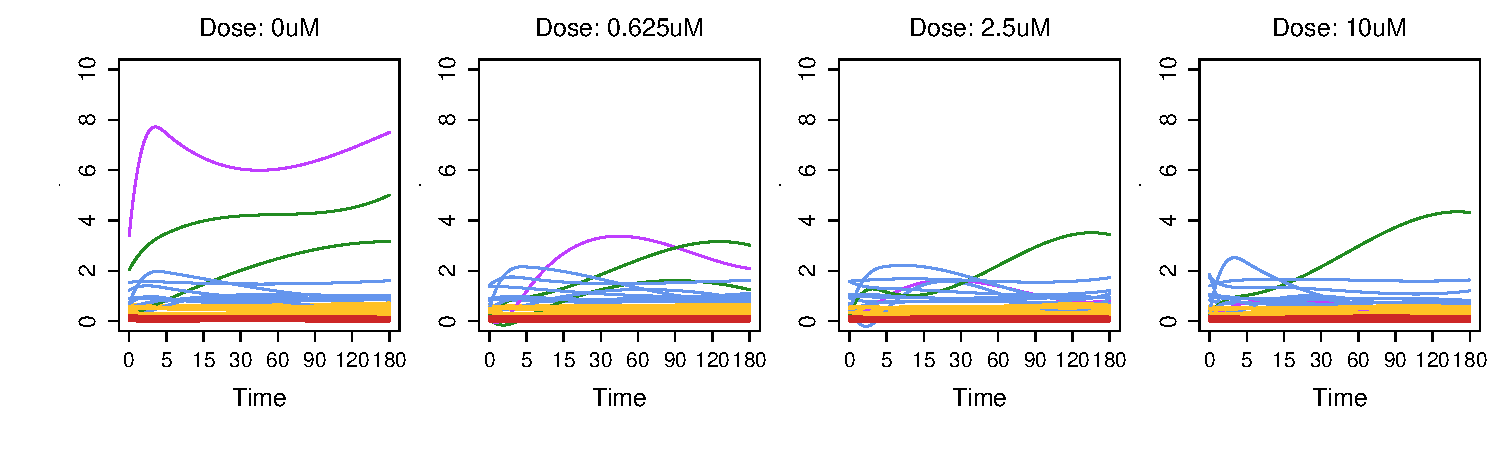
\includegraphics[scale=0.55]{figs_supporting_info/SuppInfo_ea_splines_11}
%\includegraphics[scale=0.6]{newfigs/ea_splines_11}
% \includegraphics[scale=0.6]{figs/fig5.jpeg}
\caption{Smoothing splines based on the J=3 repetitions over time (minutes) for each
protein in cell line 1 for drug PI3Ki. Cluster structure (represented in colors) is
constrained to be the same for all different doses.
Compare with the data shown in the left column of Figure 5.}
\label{fig:splines}
\end{figure}


\section{Probability Model}
\label{sec:model}

\vspace{0.5 cm}

Let $y_{cd\ell ijt}$ denote the expression level for protein $i$
in cell line $c$, drug $d$, dose $\ell$, replicate $j$ and time point $t$. To simplify notation, we drop $c$ and $d$ from the subindex in the following discussion as they appear in
(almost) all variables. Only one parameter, $\bfSigma_c$ is common across
drugs which we highlight by including the $c$ subindex for $\bfSigma_c$. In addition,
some of the hyperparameters are common across all $c,d$ as indicated below. 
We use notation for column vectors such as $(a_n)^N_{n=1} = (a_1, \ldots, a_N)^{\top}$.

We assume a model $y\lijt = \mu\lit + \epsilon\lijt,$ where $\mu\lit$ is the mean expression level for a specific cell line, drug, dose, protein and time, and $\epsilon\lijt$ represent time-dependent
Gaussian errors.
%
Let $\bfepsilon\lij = (\epsilon_{\ell ijt})^T_{t=1}$
denote the error vector. We assume $\bfepsilon_{\ell ij} \iid N(\bf0,
\bfSigma_c)$ with $\bfSigma_c$ denoting covariance matrix, independently across cell line, drugs, doses, proteins and
replicates. Similarly let $\bfy\lij = (y_{\ell ijt})^T_{t=1}$ and $\bfmu_{\ell i} = (\mu_{\ell it})^{T}_{t=1}$. The joint likelihood becomes
\begin{equation} \bfy\lij \ind N(\bfmu\li, \bfSigma_c),
  \label{eq:lik}
\end{equation} with independence across all subindex values, but dependence of the elements $y_{\ell ijt}$ across time $t=1,
\ldots, T$. We assume an inverse Wishart conjugate prior on the
covariance matrices $\bfSigma_c \ind \IW(\nu_{\Sigma}, \bfV_{\Sigma}),
\ c=1, \ldots, C,$ with expectation $\frac{\bfV_{\Sigma}}{\nu_{\Sigma}
- T - 1}$.
Here $\bfV_{\Sigma}$  is a (fixed) $T \times T$ matrix-variate hyperparameter
and $\nu_{\Sigma} \geq T + 2$ are the degrees of freedom. Introducing a more detailed model for temporal dynamics is
not meaningfully possible with the small sample sizes and only $T=8$
longitudinal observations. 

We introduce a time-dependent partition of the proteins, which
together with cluster-specific means implies a generative model for
the mean protein expressions $\bfmu\li$ within cell line, drug and
dose, and across different time points $t=1$, \ldots, $T$. We first
develop the structure for the time-dependent partitions.
Let $\bfdelta_t=(\delta_{ti})^I_{i=1}$
% \{S_{t}(1),\ldots, S_{t}(\kappa^t)\}$
denote the partition at time $t$
of proteins $i=1, \ldots, I$ into $\kappa^t$ clusters
$m=1,\ldots,\kappa^t$.
The random partitions $\bfdelta_t$ are characterized by cluster
membership indicators $\delta_{ti} \in \{1, \ldots, \kappa^t\}$ 
with $\delta_{ti} = m$ when protein $i$ is in the $m$-th cluster at time $t$.
A key model feature is the
prior probability model for the sequence of partitions
$\bfdelta_{1}, \ldots, \bfdelta_{T}$
that defines the evolution of the partitions over
time (as before, separately for each cell-line $c$ and drug $d$).
See below for the choice of $\kappa^t$ -- we will reduce it to only
two distinct values, $\kappa_1$ and $\kappa_2$, over time.
Also, for clarification we note that the dependence should be on the
partitions themselves rather than on their distributions.
Modeling the dependence on the actual proteins, i.e.,
the cluster membership of proteins, allows us to represent how the
treatment affects each protein.

One desired feature motivated by the nature of the RPPA data analysis
is that partitions should initially start fragmenting (i.e., more
subsets should be formed) up to a certain change point, after which a
coagulation process starts (i.e., merging of clusters into fewer
subsets). This reflects the drug action on proteins.  In other words,
the drug is expected to alter the regular expression pattern of the
proteins, resulting in more heterogeneous expression profiles and
therefore more clusters. As the drug effect wears off, the expression
of the proteins should revert to the original states, implying a
coagulation of the clusters.

We implement the desired structure with two change-points in time. The
first change point marks the beginning of the refined partition with more
clusters, and the second change point marks the time when the partition
reverts to the original clusters. We let $\tau^1_{\ell }$
(\textit{refinement} change point) denote the first change point when the
proteins form the finer partition, and let $\tau^2_{\ell }$
(\textit{coagulation} change point) denote the second change point.
We assume $1 \leq \tau^1_{\ell}
< \tau^2_{\ell } \leq T$ for all cell lines $c$, drugs $d$, and doses
$\ell$. One key feature is that $\tau^1_{\ell }$ and $\tau^2_{\ell}$ are
specific to dose $\ell$. This represents how different doses act
faster or slower on the proteins. Higher doses are expected to start
acting on the proteins earlier than lower doses, i.e., we expect
monotonicity of $\tau^1_{\ell}$ and $\tau^2_{\ell}$ over doses. We further
assume $
  (\tau^1_{\ell }, \tau^2_{\ell}) \iid \Unif\left(\{ (u_1, u_2): 1
\leq u_1 < u_2 \leq T-1\}\right).
$ Adding an informative prior would be straightforward. However, even
with the (vague) uniform prior we find little posterior uncertainty
on the change points.

The prior probability models for the baseline and fragmented partitions
are constructed as Dirichlet-multinomial models for cluster membership
indicators. Let $\bfdelta^u =(\delta^u_i)^I_{i=1}$ for $u\in \{1, 2\}$ denote the two partitions of
proteins with $u=1$ indicating the original (coarse) partition that applies for $t <
\tau^1_{\ell}$ and $t>\tau^2_{\ell}$, and $u=2$ indicating the (refined) partition
that applies for $\tau^1_{\ell} \leq t \leq \tau^2_{\ell}$. That is,
\begin{equation*}
\bfdelta_{t}=
\begin{cases}
  \bfdelta^1, \mbox{ for }
  1\leq t \leq \tau^1_{\ell }, \mbox{ or } t \geq \tau^2_{\ell }+1 \\
  \bfdelta^2, \mbox{ for } \tau^1_{\ell }+1 \leq t \leq \tau^2_{\ell }.
\end{cases}
\end{equation*}

We assume that 
$
P(\delta^1_i = m) = \pi^1_m
% (1), \ldots, \delta^1(I) \iid
%    \Cat(\{1,\ldots,\kappa_1\}, (\pi^1_1, \ldots, \pi^1_{\kappa_1}) ).
$
for clusters $m=1, \ldots, \kappa_1$.
The prior for the fragmented partition $\bfdelta^2$ is constructed in two steps. First, set
$\delta^2_i = \delta^1_i$ with probability $\gamma$; second, all
proteins $i$ with $\delta^2_i \not=\delta^1_i$ are gathered in the set
$\AAA:=\{i: \ \delta^1_i \neq \delta^2_i\}$, and form new
clusters by $P(\delta^2_i=m) = \pi^2_{m-\kappa_1},~ m=\kappa_1+1,\ldots,\kappa_2, \ i \in \AAA.$ Note that $p(\bfdelta^2 \mid \bfdelta^1)$ does not define $\bfdelta^2$
as a partition nested within $\bfdelta^1$.  This is why we use
the term refinement throughout. 

We assume independent priors for $\gamma$,
  $\bfpi_1=(\pi^1_1,\ldots,\pi^1_{\kappa_1})$ and
  $\bfpi_2=(\pi^2_1,\ldots,\pi^2_{\kappa_2-\kappa_1})$ as
$
   \gamma \sim \mbox{Beta}(a_\gamma, b_{\gamma})\
   \bfpi_1 \sim \Dir(\bfeta_1), \mbox{ and } \
   \bfpi_2 \sim \Dir(\bfeta_2).
$
The hyperparameters $\gamma, \bfpi_1, \bfpi_2$ are shared across all cell
lines $c$ and drugs $d$. 

Next, we construct a prior for the mean protein expression
$\bfmu\li$ in \eqref{eq:lik} by defining cluster-specific common
values.
% \bch $(\mu^*_{\ell,1}(m),\mu^*_{\ell,1}(m),\mu^*_{\ell,3}(m))$ for
% proteins in cluster $m$, under dose $\ell$ over interval $u=1,2,3$. \ech
That is, the partition is linked with the protein mean expression.
Given  $\{\bfdelta_{t}: \ 1\leq t \leq T\}$ we assume
\begin{equation}
\mu\lit=
\begin{cases}
\mu^*_{\ell 1}(\delta^1_i), \mbox{ if } 1\leq t \leq \tau^1_{\ell }\\
\mu^*_{\ell 2}(\delta^2_i), \mbox{ if } \tau^1_{\ell }+1 \leq t \leq \tau^2_{\ell }\\
\mu^*_{\ell 3}(\delta^1_i), \mbox{ if } \tau^2_{\ell }+1 \leq t.
\end{cases}
\label{eq:mu_vec}
\end{equation}
In words, $\mu\lit = \mu^*_{\ell u}(m)$ for all proteins in cluster $m$ under
dose level $\ell$ in the time interval $u=1,2$ or $3$, with the time
intervals corresponding to the initial, fragmented and final partitions respectively (initial and final partitions are assumed equal). The choice of the piecewise constant mean function in
\eqref{eq:mu_vec} is only for parsimony. Alternatively, one could use
a piecewise linear mean response, without much change in the remaining
discussion. The use of a distinct $\mu^*_{\ell 3}$, i.e. $\mu^{*}_{\ell 3}=\mu^{*}_{\ell 1}$ allows for a persisting effect of the drug intervention, short of a complete restriction to baseline.

The model is completed with a prior on the cluster-specific parameters, $  (\mu^*_{\ell u}(m)\mid \mu_{0u}, v_{0u}) \iid N(\mu_{0u}, v^{-1}_{0u}), \
  \mu_{0u} \iid  N(\mu_{00}, v^{-1}_{00}) \ \mbox{and} \
  v_{0u}   \iid  \mbox{Gamma}(a_v, b_v).$
The hyperparameters $(\mu_{0u},v_{0u})$ are common across cell lines $c$
and drugs $d$. 

In summary, the proposed model constructs a mixture of Gaussian sampling model
for the observed protein expressions over time, with the mixture being
induced by the latent partitions $\bfdelta^1$ and $\bfdelta^2$.
In fact,  marginalizing $\bfdelta^1$ and $\bfdelta^2$, we find the
following mixture of normals sampling model.
Let
$\bfu_1 = (1, \ldots, 1, 0, \ldots, 0)^{\top}$,
$\bfu_2 = (0, \ldots, 0, 1, \ldots, 1, 0, \ldots, 0)^{\top}$ and
$\bfu_3 = (0, \ldots, 0, 1, \ldots, 1)^{\top}$
denote design vectors with 1's in positions $1,\ldots,\tau^1_{\ell}$
(for $\bfu_1$), 
in positions $\tau^1_{\ell}+1, \ldots, \tau^2_{\ell}$ (for $\bfu_2$) and
in positions $\tau^2_{\ell} + 1, \ldots, T$ (for $\bfu_3$), respectively, and
let
$
\bfmu^*_{\ell}(k_1, k_2) = \mu^*_{\ell 1}\left(k_1\right)\bfu_1 +
\mu^*_{\ell 2}\left(k_2\right)\bfu_2 + \mu^*_{\ell
  3}\left(k_1\right)\bfu_3
$
denote the $T$-dimensional mean vector for proteins in clusters $k_1$
and $k_2$ under the initial and the refined partition, respectively. Let $N(\bfx;\, \bfm, \bfS)$ denote a multivariate normal p.d.f. evaluated at $\bfx$ with mean $\bfm$ and covariance matrix $\bfS$. Then
\begin{multline*}
p(\bfy_{\ell ij} \mid \tau^1_{\ell}, \tau^2_{\ell}, \bfSigma_c, 
 \bfmu^*_{\ell 1}, \bfmu^*_{\ell 2}, \bfmu^*_{\ell 3}, \bfpi_1,
 \bfpi_2, \gamma)=\\
= (1-\gamma) \sum^{\kappa_1}_{k_1=1}\sum^{\kappa_2-\kappa_1}_{k_2=1} 
   \pi^1_{k_1}\pi^2_{k_2}N(\bfy_{\ell ij} ; \bfmu^*_{\ell}(k_1, k_2), \bfSigma_c) \
+ \\ 
+\gamma \sum^{\kappa_1}_{k_1 = 1} 
   \pi^1_{k_1}N(\bfy_{\ell ij} ; \bfmu^*_{\ell}(k_1, k_1),
   \bfSigma_c). 
 \label{eq:marginal_likelihood} 
\end{multline*}

Note how the proposed model is different from models that allow dependence
of the distributions for the random partitions. 
Dependence in the prior on the random partitions over time would not necessarily
enforce the desired monotonicity of refinement (to represent the
treatment effect) and following coagulation for an actual realization
of protein-specific cluster membership.
Here, the dependence is built on the partitions themselves, unlike,
for example, the earlier 
mentioned model of \cite{caronetal:07} where each $\bfdelta_t$ is marginally
distributed according to a PY-style (Generalized P\'olya urn) distribution, 
exploring several ways to relate and control similarity across partitions.
The fragmentation
and coagulation feature cannot be represented by models with invariant
marginal distribution. Modeling the desired monotone pattern of change in
the partition is the key motivation for the proposed construction.

Finally, we would like to comment on the choice of the proposed model
versus a seemingly simpler parametric model, such as a linear mixed
effects model or a regression with splines, as in Figure 1 in the supporting information section.
While such parametric models could adequately model time-dependent
mean response, inference for protein-specific response to treatment
effects would require corresponding protein- and time-specific random
effects.

\section{Posterior Inference}
\label{sec:inference}

We implement Markov chain Monte Carlo (MCMC) posterior simulation.
Let $\bftheta$ denote the complete
parameter vector. For posterior simulation it is now important to keep
track of parameters that are in common across cell lines $c$ and drugs
$d$. We therefore start to include the subindexes $c$ and $d$ again as needed.
The joint prior distribution can be factorized as
\begin{align*}
p&(\bftheta) \propto
 \left\{\prod^3_{u=1}p(v_{0u})\right\}
 \left\{\prod^3_{u=1}p(\mu_{0u})\right\}
 \left\{\prod^C_{c=1}\prod^{D}_{d=1}\prod^L_{\ell=1} p(\tau^1_{cd\ell}, \tau^2_{cd\ell})\right\}
 p(\gamma)\\
%
&\times \left\{\prod^C_{c=1}\prod^D_{d=1}
  p(\bfdelta_{cd}^1\mid \bfpi_1)
  p(\bfdelta^2_{cd} \mid \bfdelta^1_{cd}, \gamma, \bfpi_2)\right\} \times
  p(\bfpi_1) p(\bfpi_2) \times
 \prod^{D}_{d=1} \prod^{C}_{c=1}p(\bfSigma_c)\\
%
& \times  \prod^C_{c=1} \prod^D_{d=1} \prod^L_{\ell=1}
  \left\{
  \underbrace{
  \prod^{\kappa_{1}}_{m=1}p(\mu^*_{cd\ell 1}(m) \mid \mu_{01}, v_{01})
  }_{u=1}\times
  \underbrace{
    \prod^{\kappa_{2}}_{m=1}p(\mu^*_{cd\ell 2}(m) \mid \mu_{02}, v_{02})
  }_{u=2} \times\right.\\
%
&\times \left.
  \underbrace{
    \prod^{\kappa_{1}}_{m=1}p(\mu^*_{cd\ell 3}(m) \mid \mu_{03}, v_{03})
  }_{u=3}
\right\},
\end{align*}
where $\kappa_{1}$ is the number of
clusters in time intervals $\{t: \ 1\leq t \leq \tau^1_{cd\ell}\}$ (corresponding
to $u=1$) and $\{t: \ t > \tau^2_{cd\ell}\}$ (or $u=3$); and $\kappa_2$ is the number of clusters in time interval $\{t: \ \tau^1_{cd\ell}+1\leq t \leq \tau^2_{cd\ell}\}$ (or $u=2$). 
If desired, the model could easily be generalized to different number of clusters
across cell line and drugs. The likelihood is given by the independent normal sampling model
$$
 \prod^{C}_{c=1} \prod^{D}_{d=1} \prod^{I}_{i=1} \prod^{L}_{\ell=1}
 \prod^{J}_{j=1} N( \bfy_{cd\ell ij}; \ \bfmu_{cd \ell i}, \  \bfSigma_c).
$$
Although posterior inference is not analytically tractable for this model,
conditional conjugacy implies that all full conditionals are well known
distributions that are straightforward to sample from (see Web Appendix
A). We therefore implement MCMC simulation using a Gibbs
sampler Markov chain.
We run one common Markov chain for inference across all $(c,d)$,
but report inference on partitions separately for each $(c,d)$. Therefore, in the
following discussion of inference summaries, we drop the
$_{cd}$ subindex again. 

Point estimates of the cluster-membership indicators are obtained using the
approach proposed by \cite{dahl2006}. After
judging (practical) convergence of the MCMC algorithm, we evaluate for each pair $i<j$ of
proteins, the pairwise co-clustering probability $\phat_{ij} = \frac 1K
{\sum_k} \pijk$, where $K$ is the Monte Carlo sample size and $\pijk$ is
an indicator for $i$ and $j$ being allocated to the same cluster. The
$\pijk$ and $\phat_{ij}$ are combined into $(I \times I)$ matrices
$\bfPk = [\pijk]$ and $\bfPhat = [\phat_{ij}]$. We then report as
posterior estimated $\bar{\bfdelta}$ the partition corresponding to the $\bfP^{(k^*)}$
% co-clustering matrix $\bfPs$
% cluster in iteration $k$, and 0 otherwise. Finally, the cluster
% membership indicator are punctually estimated by the $\bfP^{(k^*)}$
that minimizes $ ||\bfPhat - \bfP^{(k)} ||$, i.e.,
$
  k^\star = \arg\min_k || \hat{\bfP} - \bfP^{(k)} ||.
$
% Notice that such procedure takes the entire posterior sample into
% consideration and, since only one of those iterations is used to get
% the final point estimate for the clusters, problems with label
% switching are avoided.
In words, $k^\star$ indexes the Monte Carlo sample whose co-clustering
matrix is closest to $\bfPhat$. Once the point estimate of the
clustering structures is obtained, we run a new MCMC chain with fixed
cluster membership indicators to carry out inference for the remaining
parameters, now conditional on the estimated partition.

Finally, we consider learning about the unknown size $\kappa_1$ and
$\kappa_2$ of the partitions.
Using transdimensional transition probabilities, such as reversible jump
\citep{green1995},
the selection of these parameters could be included
in the same MCMC simulation.
However, we found that the implementation of such transition
probabilities is impractical for the proposed model. Considering a
variation of reversible jump for multivariate mixtures of normals with split and
merge proposals that are constructed to maintain marginal first and
second moments
\citep{zhang2004,Dellaportas2006}
we find it impossible to achieve acceptable mixing rates of the Markov
chain simulation. The challenge lies in finding a split move that simultaneously proposes reasonable draws for $\mu^*_{cd\ell u}(m)$ across all $\ell\in \{1, \ldots, L\}$, $u\in \{1, 2, 3\}$ and $m\in \{1, \ldots, \kappa_1\}$ with high probability. We therefore recommend to use an alternative model
selection framework to determine $(\kappa_1,\kappa_2)$.
We consider several criteria, including AIC \citep{akaike1973}, BIC
\citep{schwarz1978}, DIC \citep{spiegelhalter2002}, and WAIC
\citep{watanabe2010} as well as log pseudo marginal likelihood (LPML).
See, for example, \cite{gelman2014} for a review on these methods. The
specifics of counting the number of parameters, as it is required to
evaluate AIC and BIC are described in Web Appendix B.
In the following section we report a specific recommendation, based on
results in a simulation study. 

\section{Simulation}
\label{sec:simulation}

We carried out several simulation studies to verify that the proposed
model allows for meaningful inference in the context of weak signals
and relatively small sample sizes as in the RPPA data.  We considered
two scenarios, with several variations.
\smallskip

\underline{Scenario 1:}
We simulated five hypothetical datasets with the following
(true) partition sizes: $(\kappa_1, \kappa_2) \in \{ (2,3), (3,4), (3, 5), (4,7),
(5,7)\}$. In all five cases we simulated from the model described in
section \ref{sec:model}. The bottom level hyperparameters were fixed as
$\gamma = 0.9$, $v_{0u} = 5$ for $u = 1, 2, 3$ and $\bfSigma_c = 0.1 I_{8\times 8}$, where $I_{8\times 8}$ denotes the 8 dimensional identity matrix.
For any cell line $c$ and dose $\ell$, the change points were fixed as
$(\tau^1_{cd\ell}, \tau^2_{cd\ell}) = (2, 5)$ for $d = 1$, $(\tau^1_{cd\ell}, \tau^2_{cd\ell}) = (3, 6)$
for $d=2$ and $(\tau^1_{cd\ell}, \tau^2_{cd\ell}) = (4,7)$ for $d=3$. For
$(\kappa_1, \kappa_2) = (2,3), (3,4), (3, 5),$ we fixed $\mu_{0u} = (0.5,
1.5, 0.4),$ whereas for $(\kappa_1, \kappa_2) = (4,7), (5,7),$ we fixed
$\mu_{0u} = (1.0, 1.5, 1.4).$ The remaining parameters were randomly
generated from the respective prior probability model. 

For each dataset we then implement inference in two steps as in section
\ref{sec:inference}. First we run 500 MCMC iterations,
discarding the first 100 as initial burn-in
under each one of 21 possible pairs of $(\kappa_1,\kappa_2)$. We use the pairs
$\{(a,b): a \in \{2,\ldots, 8\}, \ b \in \{a+1, a+2, a+3\} \ \}$.
This first step evaluates the different model choice
criteria (see below) to select the best pair $(\kappa_1, \kappa_2)$,
and then estimates $(\bfdelta^1_{cd},\bfdelta^2_{cd})$ using the approach of
\cite{dahl2006}.

In a second step we simulate 5000 more MCMC iterations
to implement inference conditional on the
chosen model, i.e., with fixed
$\bfdelta^1_{cd}, \ \bfdelta^2_{cd},$ \  $c=1,2, \ d = 1,2,3$.
The first 2000 iterations are discarded as initial burn-in.
Hyperparameters are fixed
as $\nu_{\Sigma} = 10$, $\bfV_{\Sigma}=I_{8\times 8}$,
$a_{\gamma}= 1$, $b_{\gamma}= 1$, $\bfeta_1= (1,...,1)^{\top} \in
\mathbb{R}^{\kappa_1}$, $\bfeta_2=(1,...,1)^{\top} \in
\mathbb{R}^{\kappa_2 - \kappa_1}$, $\mu_{00}=0$, $v^{-1}_{00}=0.4444$,
$a_v=1$ and $b_v=1$ to reflect weak prior information.

We implement learning about the cluster sizes
$(\kappa_1,\kappa_2)$ as model selection using various criteria
proposed in the literature. We briefly summarize the results in Table
\ref{tab:IC}. BIC always selects a more parsimonious model, and AIC, DIC,
WAIC and LPML always point to the same model (except under $(5,7)$). We
conclude to use BIC, as it gives the best trade-off of a good fit and
selecting parsimonious models.


\begin{table}[tbp]
\caption{Simulation truth and estimate for $(\kappa_1,\kappa_2)$ under
  alternative model selection criteria.
  $^\star$ Under simulation truth $(5,7)$, AIC selects $(5,6)$.
}
\centerline{
  \begin{tabular}{l|ccccc} % |
%% no clue what's going on -- my emacs needs a second "|" lest it
%% messes up color coding of the latex source :-)
    truth & (2,3) & (3,4) & (3,5) & (4,7) & (5,7)\\
    \hline
    BIC   & (2,5) & (2,5) & (3,4) & (3,6) & (5,6)\\
    AIC, DIC,WAIC, LPML & (4,7) & (3,6) & (5,6) & (4,7) & (8,10)$^\star$
  \end{tabular}
}
\label{tab:IC}
\end{table}



Next we summarize results for the simulation scenario with true $(\kappa_1, \kappa_2) \\ = (3,
5)$. In this case BIC selects $(\kappa_1, \kappa_2) = (3, 4)$. The objective is to explore whether inference can
recover mean parameters and cluster structure for data with sample
sizes and complexity comparable to the motivating RPPA study.
%  demonstrate that the inference
% procedure is capable of reasonably estimating the mean parameters and
% cluster structure under the hypothesis that data comes from the model,
% with the same sample size as the dataset analyzed in section
% \ref{sec:results}.
Figure \ref{fig:simulation_cluster_membership} shows
estimated partitions under coagulation and refinement,
arranged by cell line and drug
$(c,d)$. In a few cases, we get estimates that merge two (true)
clusters together (e.g., in the estimated partitions $\bfdelta^1_{cd}$
and $\bfdelta^2_{cd}$ for $(c,d)=(1,3)$ and for $(c,d) = (2,1)$).
% $\delta^1_{13}, \delta^1_{2,1}$).
In most cases, however, the underlying cluster structure is accurately
recovered and we are able to correctly identify which proteins
are affected by the respective drug (proteins corresponding to darkest shades of gray in plot (b)).

\begin{figure}[tbp]
  \begin{center}
  \begin{tabular}{cc}
     Cell line 1 \hspace{0.5 cm} Cell line 2 & 
     Cell line 1 \hspace{0.5 cm} Cell line 2\\
    \rotatebox{90}{drug 1 \hspace{0.1cm} drug 2 \hspace{0.1cm} drug 3}
    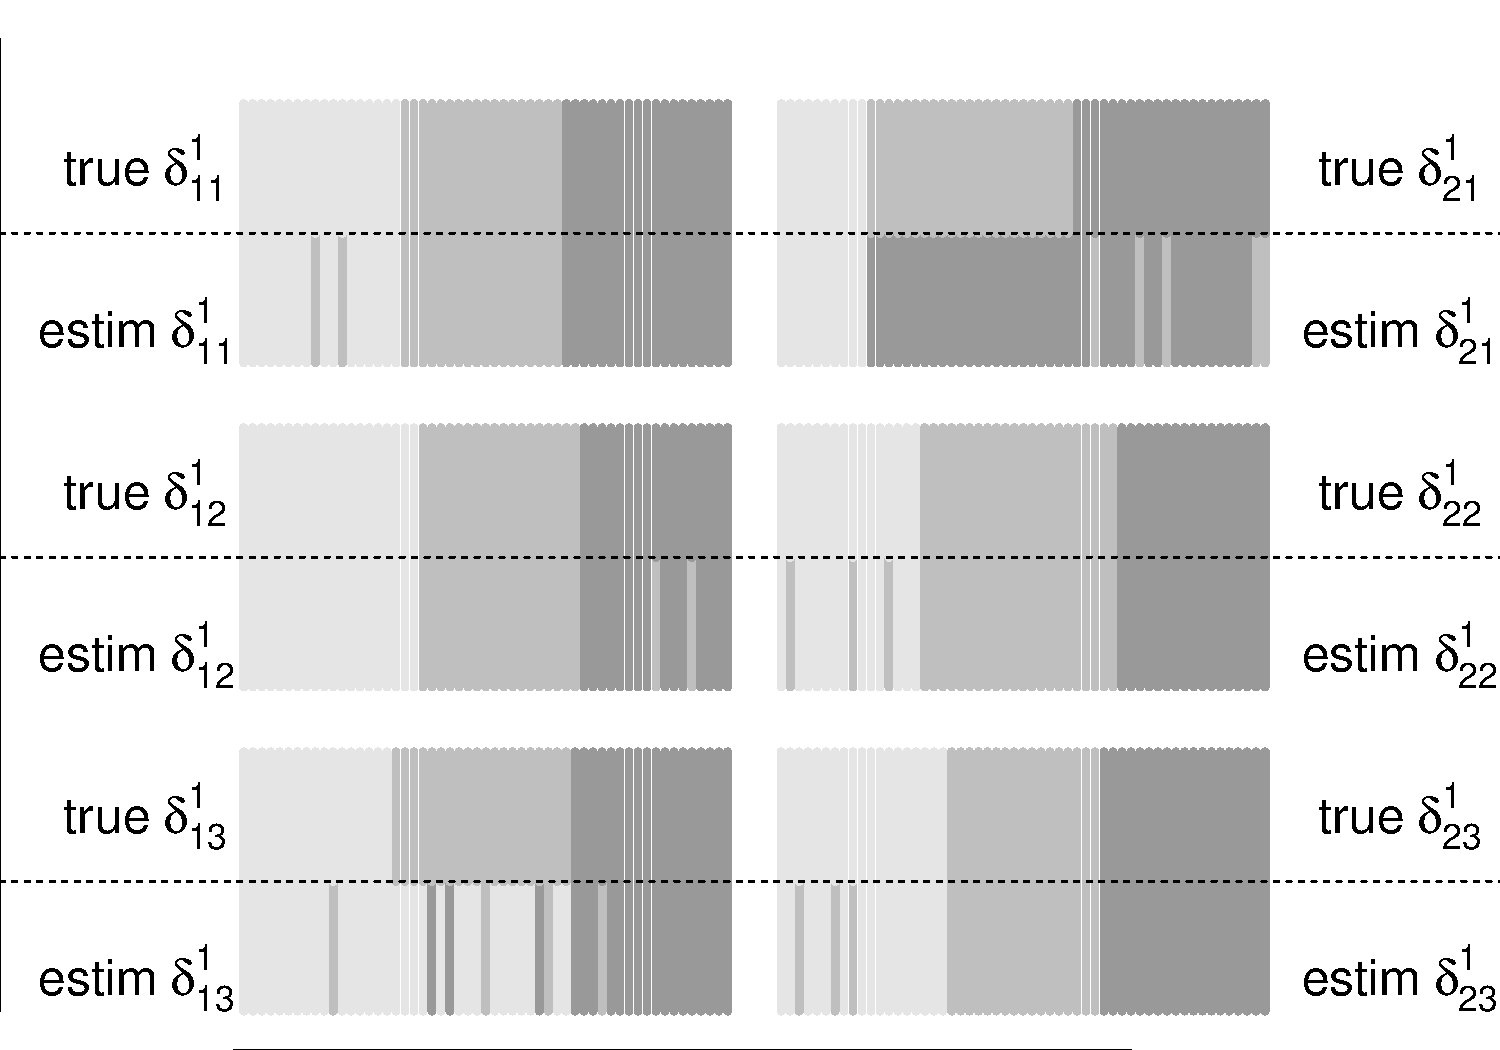
\includegraphics[width=.4\textwidth]{figs_biometrics/cluster_membership_delta1.pdf}
    &
    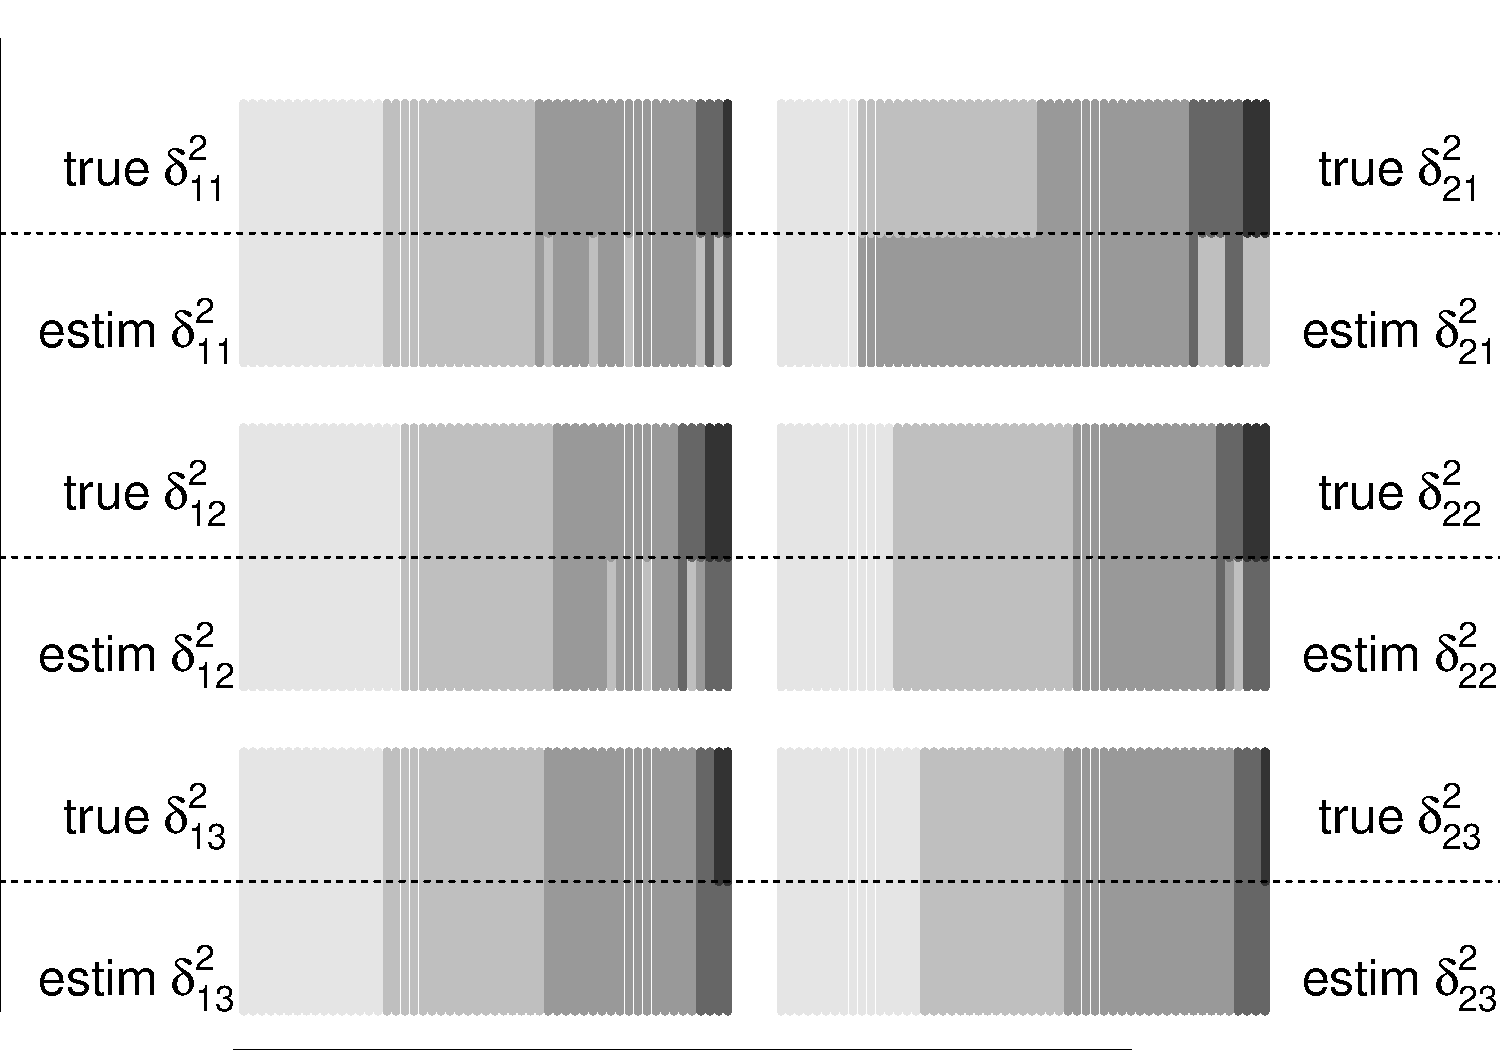
\includegraphics[width=.4\textwidth]{figs_biometrics/cluster_membership_delta2.pdf}\\
    \hspace{0.8 cm} proteins \hspace{0.5cm} proteins &
    proteins \hspace{1cm} proteins \\[4pt]
    (a) Coagulation: $t\leq \tau^1_{cd\ell},$ \ $t > \tau^2_{cd\ell}$& (b) Refinement: \ $\tau^1_{cd\ell} < t \leq \tau^2_{cd\ell}$\\[.5cm]
  \end{tabular}
  % \rotatebox{90}{\hspace{5cm} clusters}\\
  \end{center}
  \caption{Scenario 1:
    Simulation truth $\delta^u_{cd}$ (above horizontal lines) and posterior
    estimated $\deltabar^u_{cd}$ (bellow horizontal lines).
    Each vertical bar corresponds to a gene, with colors (grayscale)
    representing their respective estimated cluster memberships.}
  \label{fig:simulation_cluster_membership}
\end{figure}

Figure \ref{fig:mean_curves_simulation} shows estimated cluster membership and
mean responses (first two columns) in comparison with the
simulation truth (last two columns) for one specific combination of cell
line and drug $(c=2,d=3)$.
Comparing the simulation truth in column 4 with the estimated means in
column 2 we find a good fit for the data.
With one less cluster in the refinement stage picked by BIC, the model merges the two new clusters (darkest shades of gray in columns 3 and 4) into only one
(darkest shade of gray in columns 1 and 2), still providing a good fit with a more parsimonious model.


\begin{figure}[tbp]
%\begin{center}
 \hspace{1.5cm} $\ybar_{it}$ by $\hat{\delta}$ \hspace{0.8cm}
  $E(\mu^*_{\ell u}(m) \mid y,\hat{\delta})$     \hspace{.8cm}
  $\ybar_{it}$ by true  $\delta$           \hspace{.81cm} 
  true $\mu^*_{\ell,u}(m)$\\
  \rotatebox{90}{\hspace{.5cm} dose $\ell=3$ \hspace{1.5cm}
                               $\ell=2$ \hspace{1.5cm}
                               $\ell=1$ \hspace{1.5cm}
                               $\ell=0$                             }
  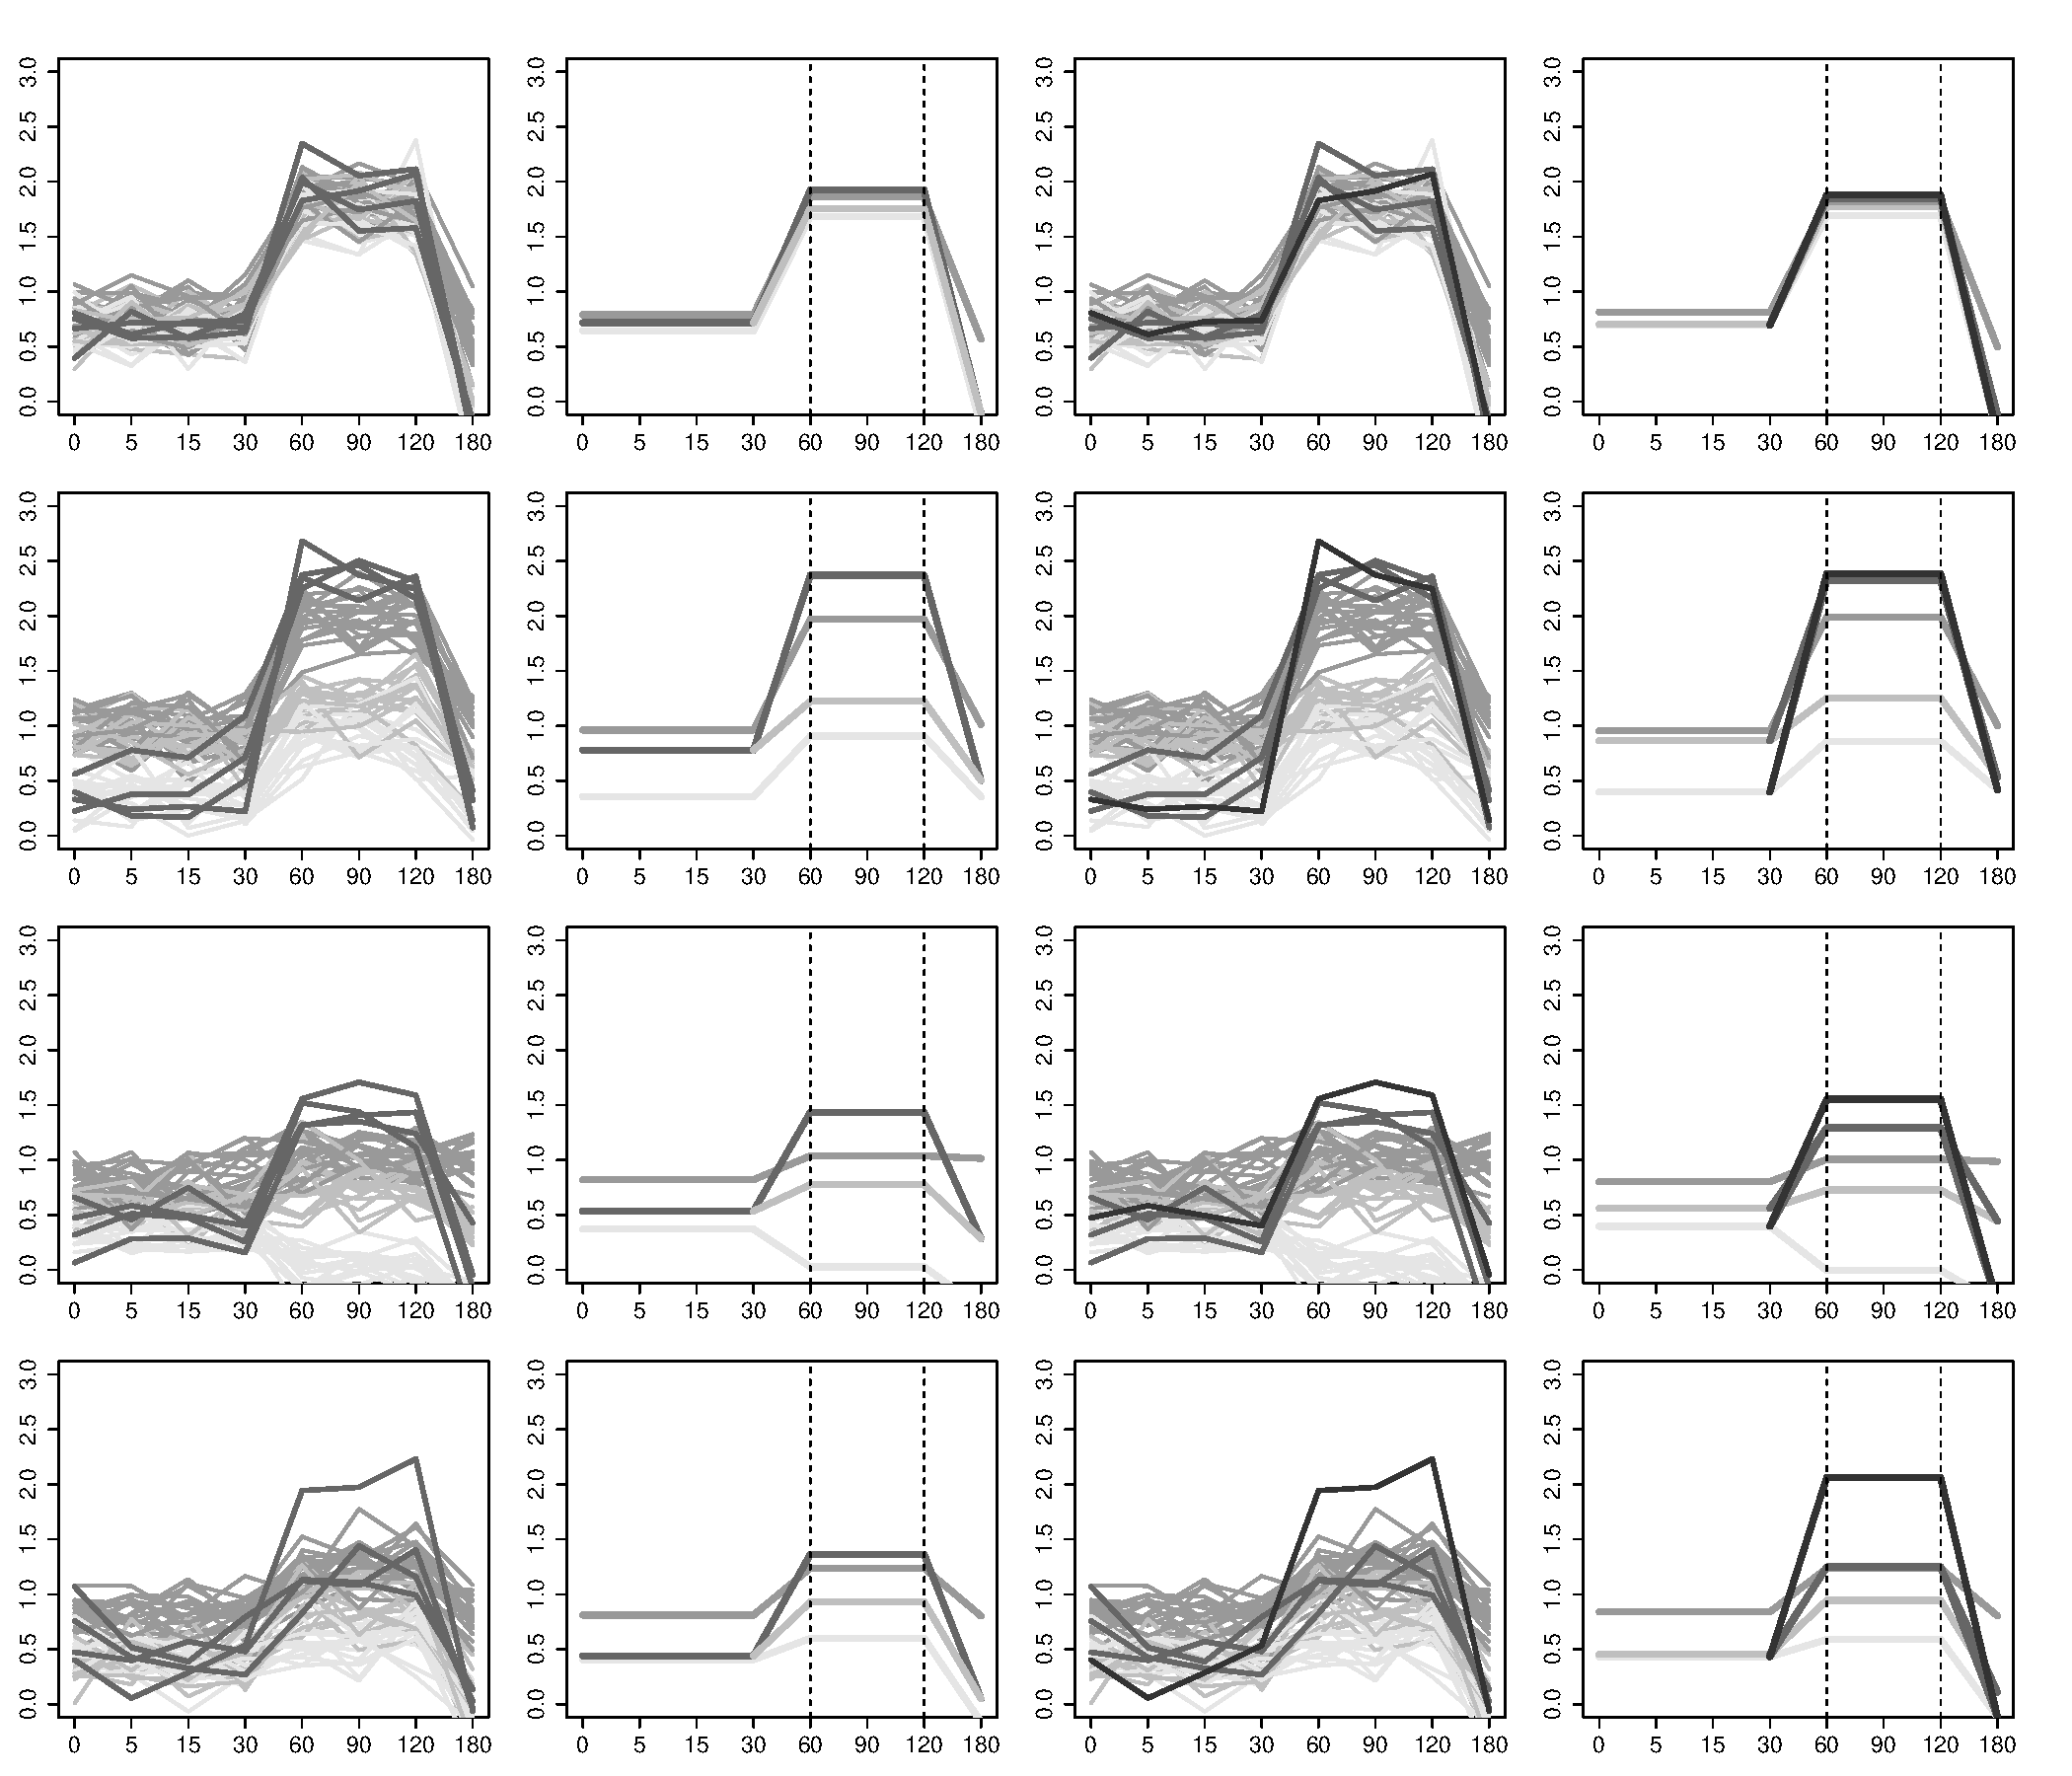
\includegraphics[scale=0.4]{figs_biometrics/sim_35_scenario1_23.pdf} \\
%  \includegraphics[scale=0.4]{figs_biometrics/results_cc_2_d_3_ver3} \\
% \end{center}  
  
\caption{Scenario 1: Mean-response estimation for one of the simulated cases (cell
  line 2, drug 3). Each row corresponds to a different (increasing) dosage level.
  Time is measured in minutes on the horizontal axis.  Column 1 and 3: average over repetitions,
  $\ybar_{it} = \frac{1}{J}\sum^J_{j=1}
  y_{\ell ijt}$ for the 55 proteins. Each line corresponds to a specific
  protein and the color (grayscale) indicates the posterior estimated cluster
  (column 1) and the true cluster (column 3).  Column 2 and 4: posterior
  estimates (column 2) and simulation truth (column 4) for $\mu_{i\ell
    t}$ with dashed lines denoting
  estimated refinement and coagulation times $\tau^1_{\ell}$ and
  $\tau^2_{\ell}$. }
 \label{fig:mean_curves_simulation}
\end{figure}
%\note{Caption: Each row is a different dose (the last row is NOT the average of the previous ones) -- C}

\underline{Scenario 1a. }
We explore prior sensitivity with respect to
the prior on the random partitions and the structure of partitions
over time.
We first repeat inference, still with the same data as in scenario 1; but with a different
hyperprior on the random partition, namely 
$\bfpi_1 \sim \Dir (0.1, \ldots, 0.1)$ and 
$\bfpi_2 \sim \Dir(0.1, \ldots, 0.1)$.
Comparing Figure \ref{fig:sc1ab}(a) with the second column of Figure
\ref{fig:mean_curves_simulation} we find no difference with respect to
the estimated mean responses. 


\begin{figure}[tbp]
  \begin{center}
    %\includegraphics[width=.9\textwidth]{figs_biometrics/sim35_dir_y_23}
  %\rotatebox{90}{\hspace{1.5cm}~  $\ybar_{it}$ by $\hdelta$ }\\
  % \\[4pt]
%    \includegraphics[width=.9\textwidth]{figs_biometrics/sim35_dir_mu_23} %\\[4pt]    
    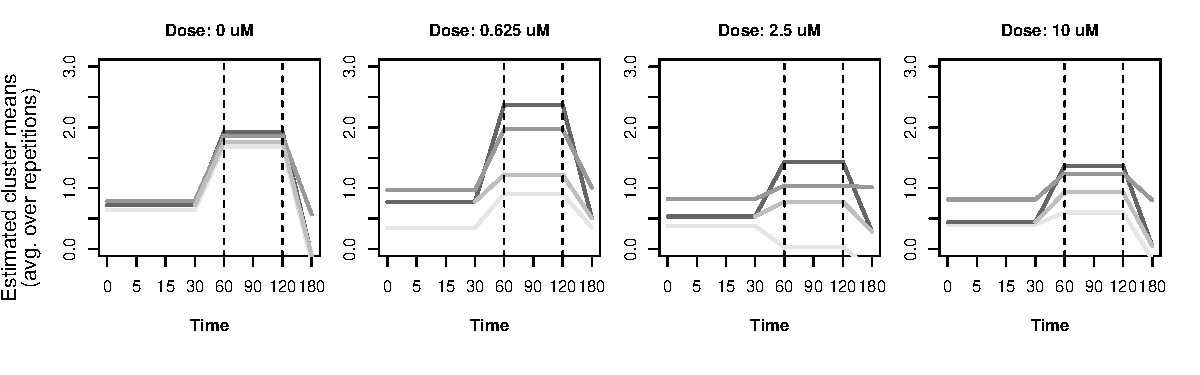
\includegraphics[width=.9\textwidth]{figs_biometrics/sim35_1a_gray_biom23.pdf} %\\[4pt]    
  \rotatebox{90}{\hspace{0.8cm}~$E(\mu^*_{\ell u}(m) \mid y,\hat{\delta})$ }\\
    (a) $\bfpi_1 \sim \Dir(0.1, \ldots, 0.1)$ 
    and $\bfpi_2 \sim \Dir(0.1, \ldots, 0.1)$.\\
    \vspace{1.0cm}
    % (a) $\pi_1 \sim \Dir ( \underbrace{0.1, ..., 0.1}_{\kappa_1})$ \ \ $\pi_2 \sim \Dir(\underbrace{0.1, ..., 0.1}_{\kappa_2 - \kappa_1})$.\\[4pt]
    %\includegraphics[width=.9\textwidth]{figs_biometrics/sim35_gamma_y_23.pdf}
  %\rotatebox{90}{\hspace{1.5cm}~  $\ybar_{it}$ by $\hdelta$ }\\
    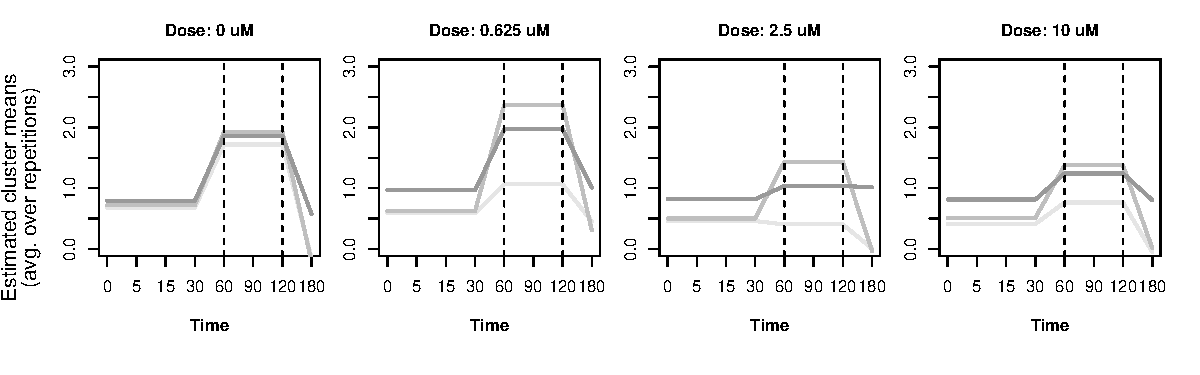
\includegraphics[width=.9\textwidth]{figs_biometrics/sim35_1b_means_23.pdf}
  \rotatebox{90}{\hspace{0.8cm}~$E(\mu^*_{\ell u}(m) \mid y,\hat{\delta})$ }\\
    (b) Single partition model: $\bfdelta^2_{cd}=\bfdelta^1_{cd}$.
  \end{center}

\caption{Scenarios 1a and 1b: Inference under two variations of the prior
  model. Colors (grayscale) denote estimated clusters.
  Panel (a) shows inference under an alternative hyperprior with a
  symmetric Dirichlet prior, 
  $\bfpi_1 \sim \Dir(0.1,\ldots, 0.1)$ and
  $\bfpi_2 \sim \Dir(0.1,\ldots, 0.1)$.
  Panel (b) shows inference 
  using a single invariant partition of proteins over time, i.e.,
  $\bfdelta^2_{cd}=\bfdelta^1_{cd}$.}
\label{fig:sc1ab}
\end{figure}

\underline{Scenario 1b. }
Alternatively we consider inference under a single random partition
that remains invariable over time, that is, using
$\bfdelta^2_{cd}=\bfdelta^1_{cd}$ for all $c$ and $d$, but still allowing changing mean levels over time
as in \eqref{eq:mu_vec}.
Figure \ref{fig:sc1ab} summarizes the resulting inference by showing the
simulated data and the estimated clusters, using the same format as
first and fourth columns in Figure  \ref{fig:mean_curves_simulation}.
Comparing Figure \ref{fig:sc1ab}(b) with the second column of Figure
\ref{fig:mean_curves_simulation} shows a substantially deteriorated
fit under the reduced model without the refined partition.
\smallskip



\underline{Scenario 2:}
We consider another hypothetical scenario with a simulation truth that
closely mimicks the estimated effects in the actual RPPA data
analysis. 
The data $y_{cdi\ell j t}$ are simulated with parameters
fixed at the posterior estimates obtained in section \ref{sec:results}, with $(\kappa_1, \kappa_2)=(4,6)$.
%
Figure \ref{fig:sc2} summarizes simulation results for $c=2$ and $d=1$. 
Using the BIC criterion we select $(\kappa_1,\kappa_2)=(4,6)$,
matching the simulation truth (with $(\kappa_1,\kappa_2)=(4,7)$ and
$(5,6)$ being second and third best). Overall, the cluster-specific means are accurately estimated and
the model fits the simulated data, indicating that inference under
the proposed model can report meaningful summaries for the motivating RPPA data.

\begin{figure}[tbp]
\begin{center}
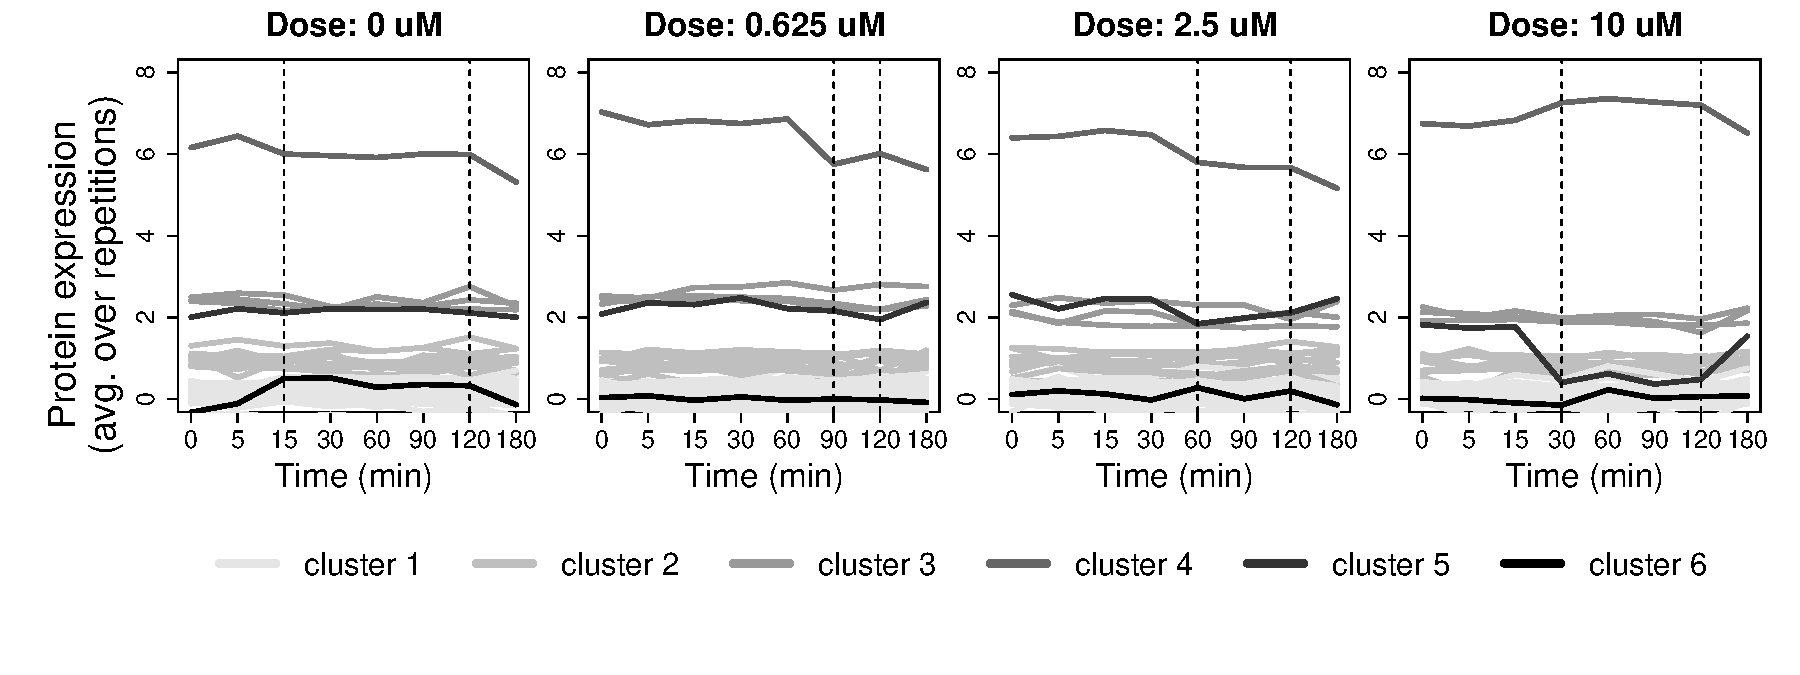
\includegraphics[width=.95\textwidth]{figs_biometrics/scenario2_y_gray_21}\\
(a) Simulated data (over 4 doses). Data for each protein is shown as a
connected line over time. Colors (grayscale) indicate cluster membership
under the simulation truth.\\[4pt]
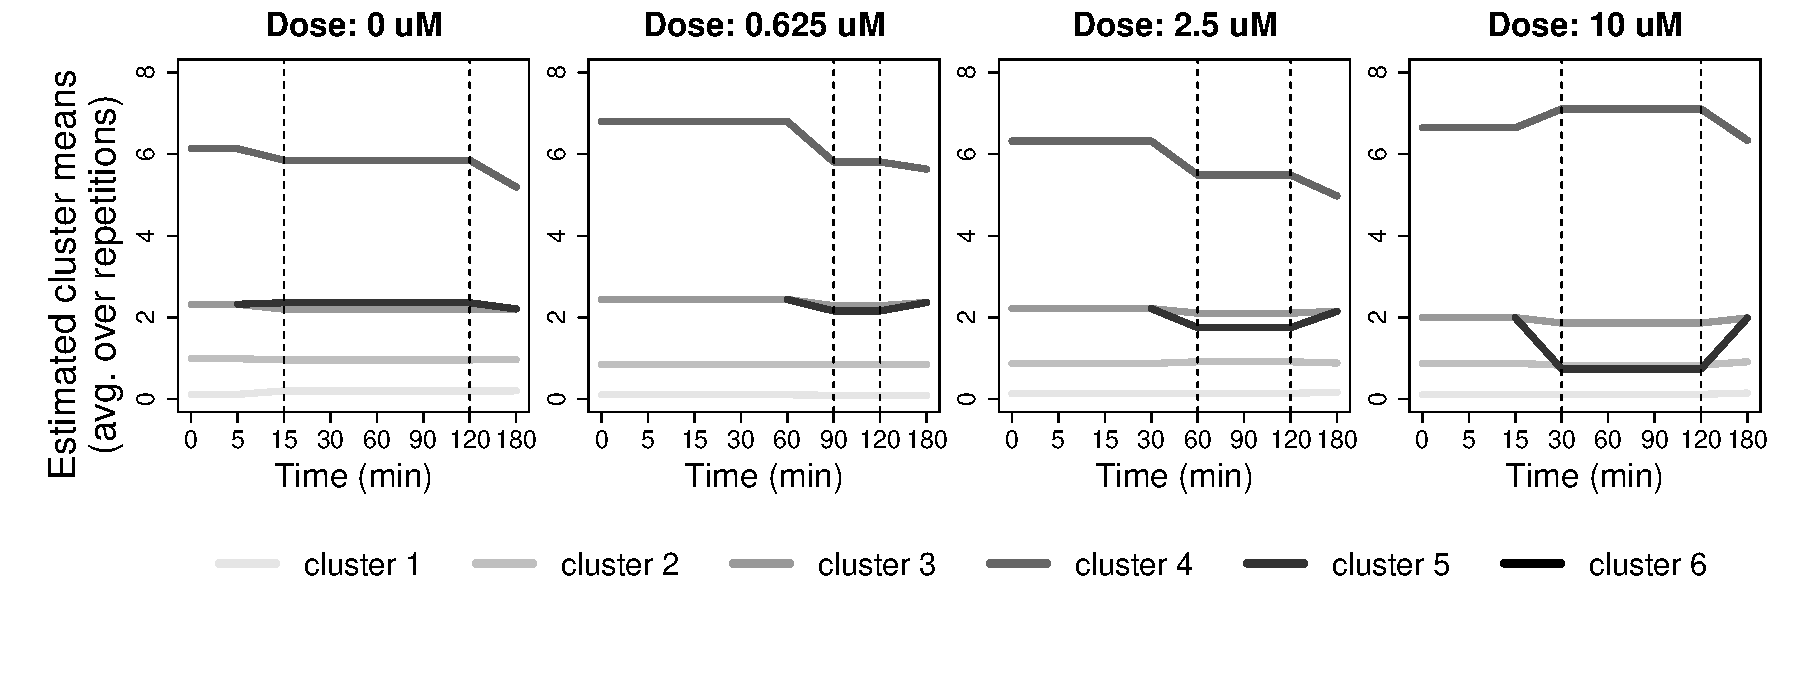
\includegraphics[width=.95\textwidth]{figs_biometrics/scenario2_means_gray_21}\\
(b) Estimated mean expression and cluster memberships. Colors (grayscale) indicate estimated cluster structure.
\end{center}
\caption{Scenario 2. Data (panel a) and estimated mean response and
  cluster membership (panel b).}
\label{fig:sc2}
\end{figure}


\section{Proteomics Data}
\label{sec:results}

Based on BIC we select  $(\kappa_1,\kappa_2)=(4,6)$ (Figure \ref{fig:bic}). While more complex models (with more clusters) exhibit
even better BIC, we find that the results for those models remain very
similar to the ones obtained under $(4,6)$, but with several empty and
redundant clusters. We therefore proceed with the more parsimonious model.

\begin{figure}[tbp]
\centering
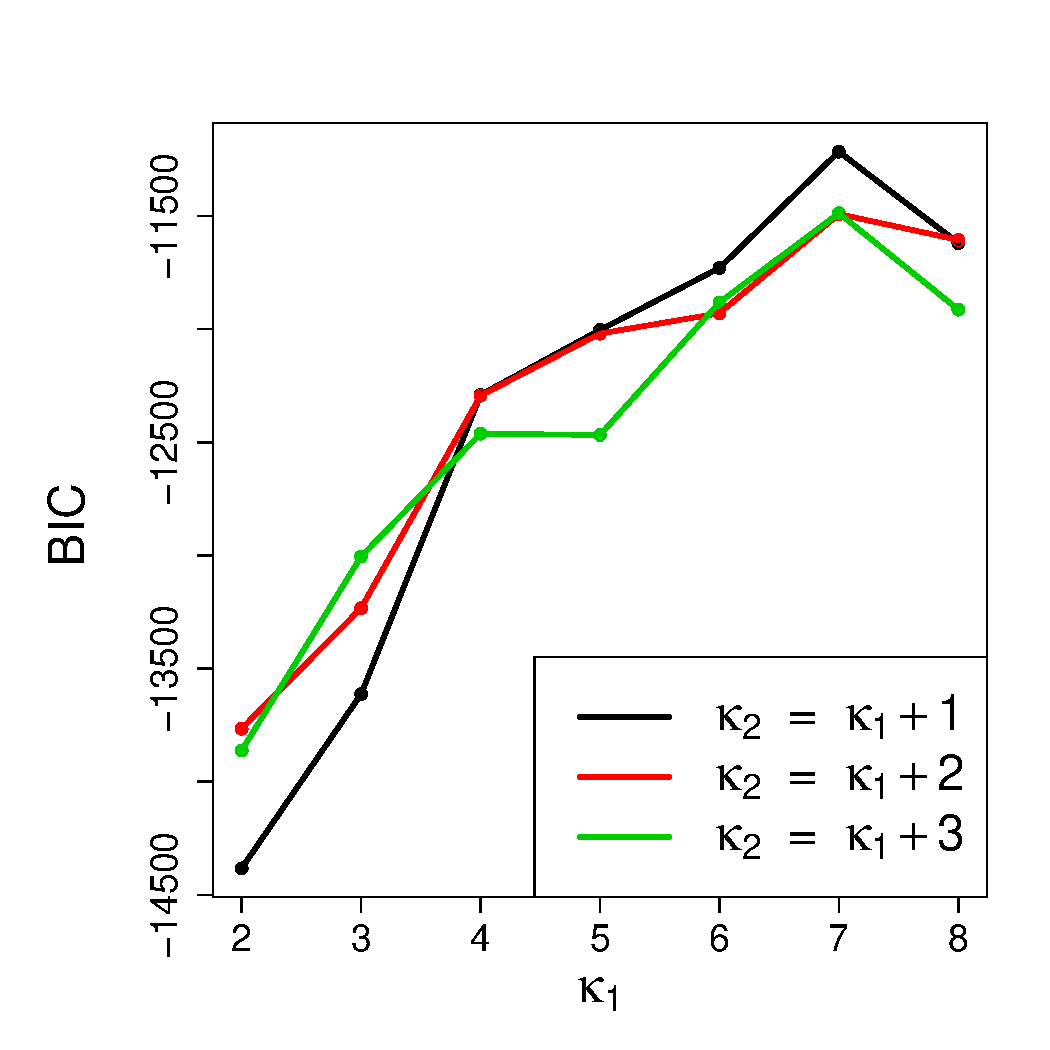
\includegraphics[scale=0.3]{figs_supporting_info/SuppInfo_model_comparison_bic.pdf}
\caption{BIC for different number of clusters $\kappa_1$ and $\kappa_2$ (the bigger, the better).}
\label{fig:bic}
\end{figure}


We implement MCMC simulation for 5,000 iterations discarding the first
2,000 as initial burn-in. Hyperparameters
are fixed as in the simulation study under Scenario 1, i.e.,
$\nu_{\Sigma} = 10$, $\bfV_{\Sigma}=I_{8\times 8}$,
$a_{\gamma}= 1$, $b_{\gamma}= 1$, $\bfeta_1= (1,...,1)^{\top} \in
\mathbb{R}^{\kappa_1}$, $\bfeta_2=(1,...,1)^{\top} \in
\mathbb{R}^{\kappa_2 - \kappa_1}$, $\mu_{00}=0$, $v^{-1}_{00}=0.4444$,
$a_v=1$ and $b_v=1$.



Figures \ref{fig:result_c1_d1} and \ref{fig:result_c2_d1}  show
estimates of the effect of PI3K 
inhibitor on the 55 proteins in cell lines 1 and 2 over time,
respectively.
Cell  line 1 is the cell line MDA-MB-231 and cell line 2 is
MDA-MB-468. Both are derived from a 51-year-old caucasian woman with 
metastatic breast cancer. The two cell lines have been shown to
respond differently to chemotherapies and hormone therapies. Here, the
goal is to characterize response to PI3K inhibition. The following discussion highlights related inference
summaries. Keeping in mind the context of this analysis in the
early phase of a drug development and the moderate sample
sizes, inference should be  understood as hypothesis generating, and
findings should not be over-interpreted.

The first two columns in both figures are as in Figure
\ref{fig:mean_curves_simulation} and show the model fit to the data.
Going from top to bottom (increasing dose) in Figure
\ref{fig:result_c1_d1} one can see that protein
S6 pS235/236
decreases with increased  PI3Ki dose.
At the same time HER2 is activated by the PI3K inhibitor. These two genes
form singletons in our analysis. The inhibition of S6 and activation
of HER2 after PI3K inhibition have been well
reported in the literature
\citep{podsypanina2001inhibitor,serra2011pi3k}. Our analysis for cell
line 1, MDA-MB-231 confirms these findings. In addition, we see
that MAPK pT202Y204 is activated in this cell line as a result of PI3K
inhibition.
We see increased MAPK expression 5 minutes after the PI3K inhibitor is
applied to the samples.
The activation of MAPK as a result of PI3K inhibition is
a major known discovery  in breast cancer~\citep{liu2009targeting}. 

In
contrast, results are different in cell line 2, MAD-MB-468  (Figure
\ref{fig:result_c2_d1}). MAPK is briefly inhibited by
the PI3K inhibitor instead of being activated as in cell line
1. This suggests that cell line 2 includes a mechanism that might reverse the
interactions of PI3K and MAPK. Due to large and complex
down-stream pathways regulated by PI3K, the effects of its inhibition
can be tissue-dependent 
and heterogeneous \citep{engelman2009targeting}. This is shown in the
different response of protein expression in the two cell lines of this
RPPA experiment. The differential response of MAPK to PI3K inhibition
across the two cell lines could be important in interpreting the
reason why they respond differently to therapies.
Discoveries like this are expected to help biologists to set up new hypothesis for further testing.

Summarizing the refinement at time $\tau^1$ as a distance between
$\delta^1$ and $\delta^2$ one could use, for example, the Hamming
distance between co-clustering matrices $P^1$ and $P^2$ with entries
$P^1_{ij}=I(\delta^1_i=\delta^1_j)$ and
$P^2_{ij}=I(\delta^2_i=\delta^2_j)$ respectively.  We find relative
(to the number of pairs) Hamming distances between the partitions
$\delta^1_{cd}$ and $\delta^2_{cd}$ to range from $0.01$ to $0.03$
depending on the cell line $c$ and drug $d$.
% For comparison, the Hamming distance
% evaluated on arbitrary partitions with $I=55$ proteins can assume any
% integer value from 0 to $55\times54/2 = 1485$. 

Table \ref{table_taus} shows point estimates for the refinement and
coagulation times $\tau^1_{\ell }$ and $\tau^2_{\ell }$,
respectively.
For cell line 1 the three drugs (columns) behave similarly,
causing the proteins to refine and revert to te baseline with a similar delay,
% and coagulate at similar time points,
without apparent dose effects. Cell line 2 is different from cell line
1 in that the cells in this line react heterogeneously to the three drugs and
doses. In particular, cell line 1 seems to be more robust to the drugs as the
refinement period is very short across doses. That is, the proteins in
this cell line in general do not react to the drugs. For cell line 2,
proteins seem to be more sensitive to the drugs.  For the first three dose
levels, 0, 0.625, and 2.5 $\mu M$, refinement starts earlier and ends
later with increasing dose levels. This is expected as higher doses
will lead to quick reaction and longer duration of the biological
system. Dose level 10 $\mu M$ is an outlier with a very short
refinement period again. This might be due to the high 
potency of the high drug concentration (10 $\mu M$ is the highest dose level).

\begin{table}[tbp]
\centering \caption{Estimated (mode) refinement and coagulation times
(minutes): $\tau_{\ell }^u$ for cell line $c$, drug $d$, dose $\ell$ and $u
\in \{1, 2\}$.} \label{table_taus}
\resizebox{\columnwidth}{!}{%
\begin{tabular}{c|cccccc|cccccc}
\multicolumn{1}{l |}{}  & \multicolumn{6}{c|}{cell line 1} & \multicolumn{6}{c}{cell line 2} \\ \cline{1-13}
\multicolumn{1}{c|}{drug}  & \multicolumn{2}{c}{PI3Ki} & \multicolumn{2}{c}{AKTi} & \multicolumn{2}{c|}{MEKi} & \multicolumn{2}{c}{PI3Ki} & \multicolumn{2}{c}{AKTi} & \multicolumn{2}{c}{MEKi} \\ \cline{1-13}
\multicolumn{1}{c|}{dose/time}          & \multicolumn{1}{c}{refin.} & \multicolumn{1}{c}{coag.} & \multicolumn{1}{c}{refin.} & \multicolumn{1}{c}{coag.}& \multicolumn{1}{c}{refin.} & \multicolumn{1}{c|}{coag.}& \multicolumn{1}{c}{refin.} & \multicolumn{1}{c}{coag.}& \multicolumn{1}{c}{refin.} & \multicolumn{1}{c}{coag.}& \multicolumn{1}{c}{refin.} & \multicolumn{1}{c}{coag.} \\ \cline{1-13}
\multicolumn{1}{c|}{0 uM}     & 0            & 15           & 0            & 5           & 0            & 15           & 60            & 120           & 60            & 90           & 5            & 120           \\
\multicolumn{1}{c|}{0.625 uM} & 0            & 15           & 0            & 5           & 0            & 5           & 60            & 90           & 5            & 90           & 60            & 120           \\
\multicolumn{1}{c|}{2.5 uM}   & 0            & 30           & 0            & 5           & 0            & 5           & 30            & 120           & 5            & 120           & 15            & 90           \\
\multicolumn{1}{c|}{10 uM}    & 0            & 30           & 5            & 30           & 0            & 5           & 0            & 30           & 90            & 120           & 30            & 60
\end{tabular}%
}
\end{table}

\begin{figure}[tbp]
% \rotatebox{90}{\hspace{4cm} $\ybar_{it}$ (1st column) and $\mu_{i\ell t}$
%   (2nd column)}
%   \hspace{-.2cm}
\phantom{xx} 
\hskip 2cm $\ybar_{it}$ by $\hat{\delta}$  \hspace{0.8cm} $E(\mu^*_{\ell t}(m)\mid y, \hat{\delta})$
  \hspace{0.9cm} coagulation \hspace{0.9cm} refinement\\
  \rotatebox{90}{\hspace{2cm}dose $\ell=3$ \hspace{1.5cm}
                               $\ell=2$ \hspace{2cm}
                               $\ell=1$ \hspace{2cm}
                               $\ell=0$                             }
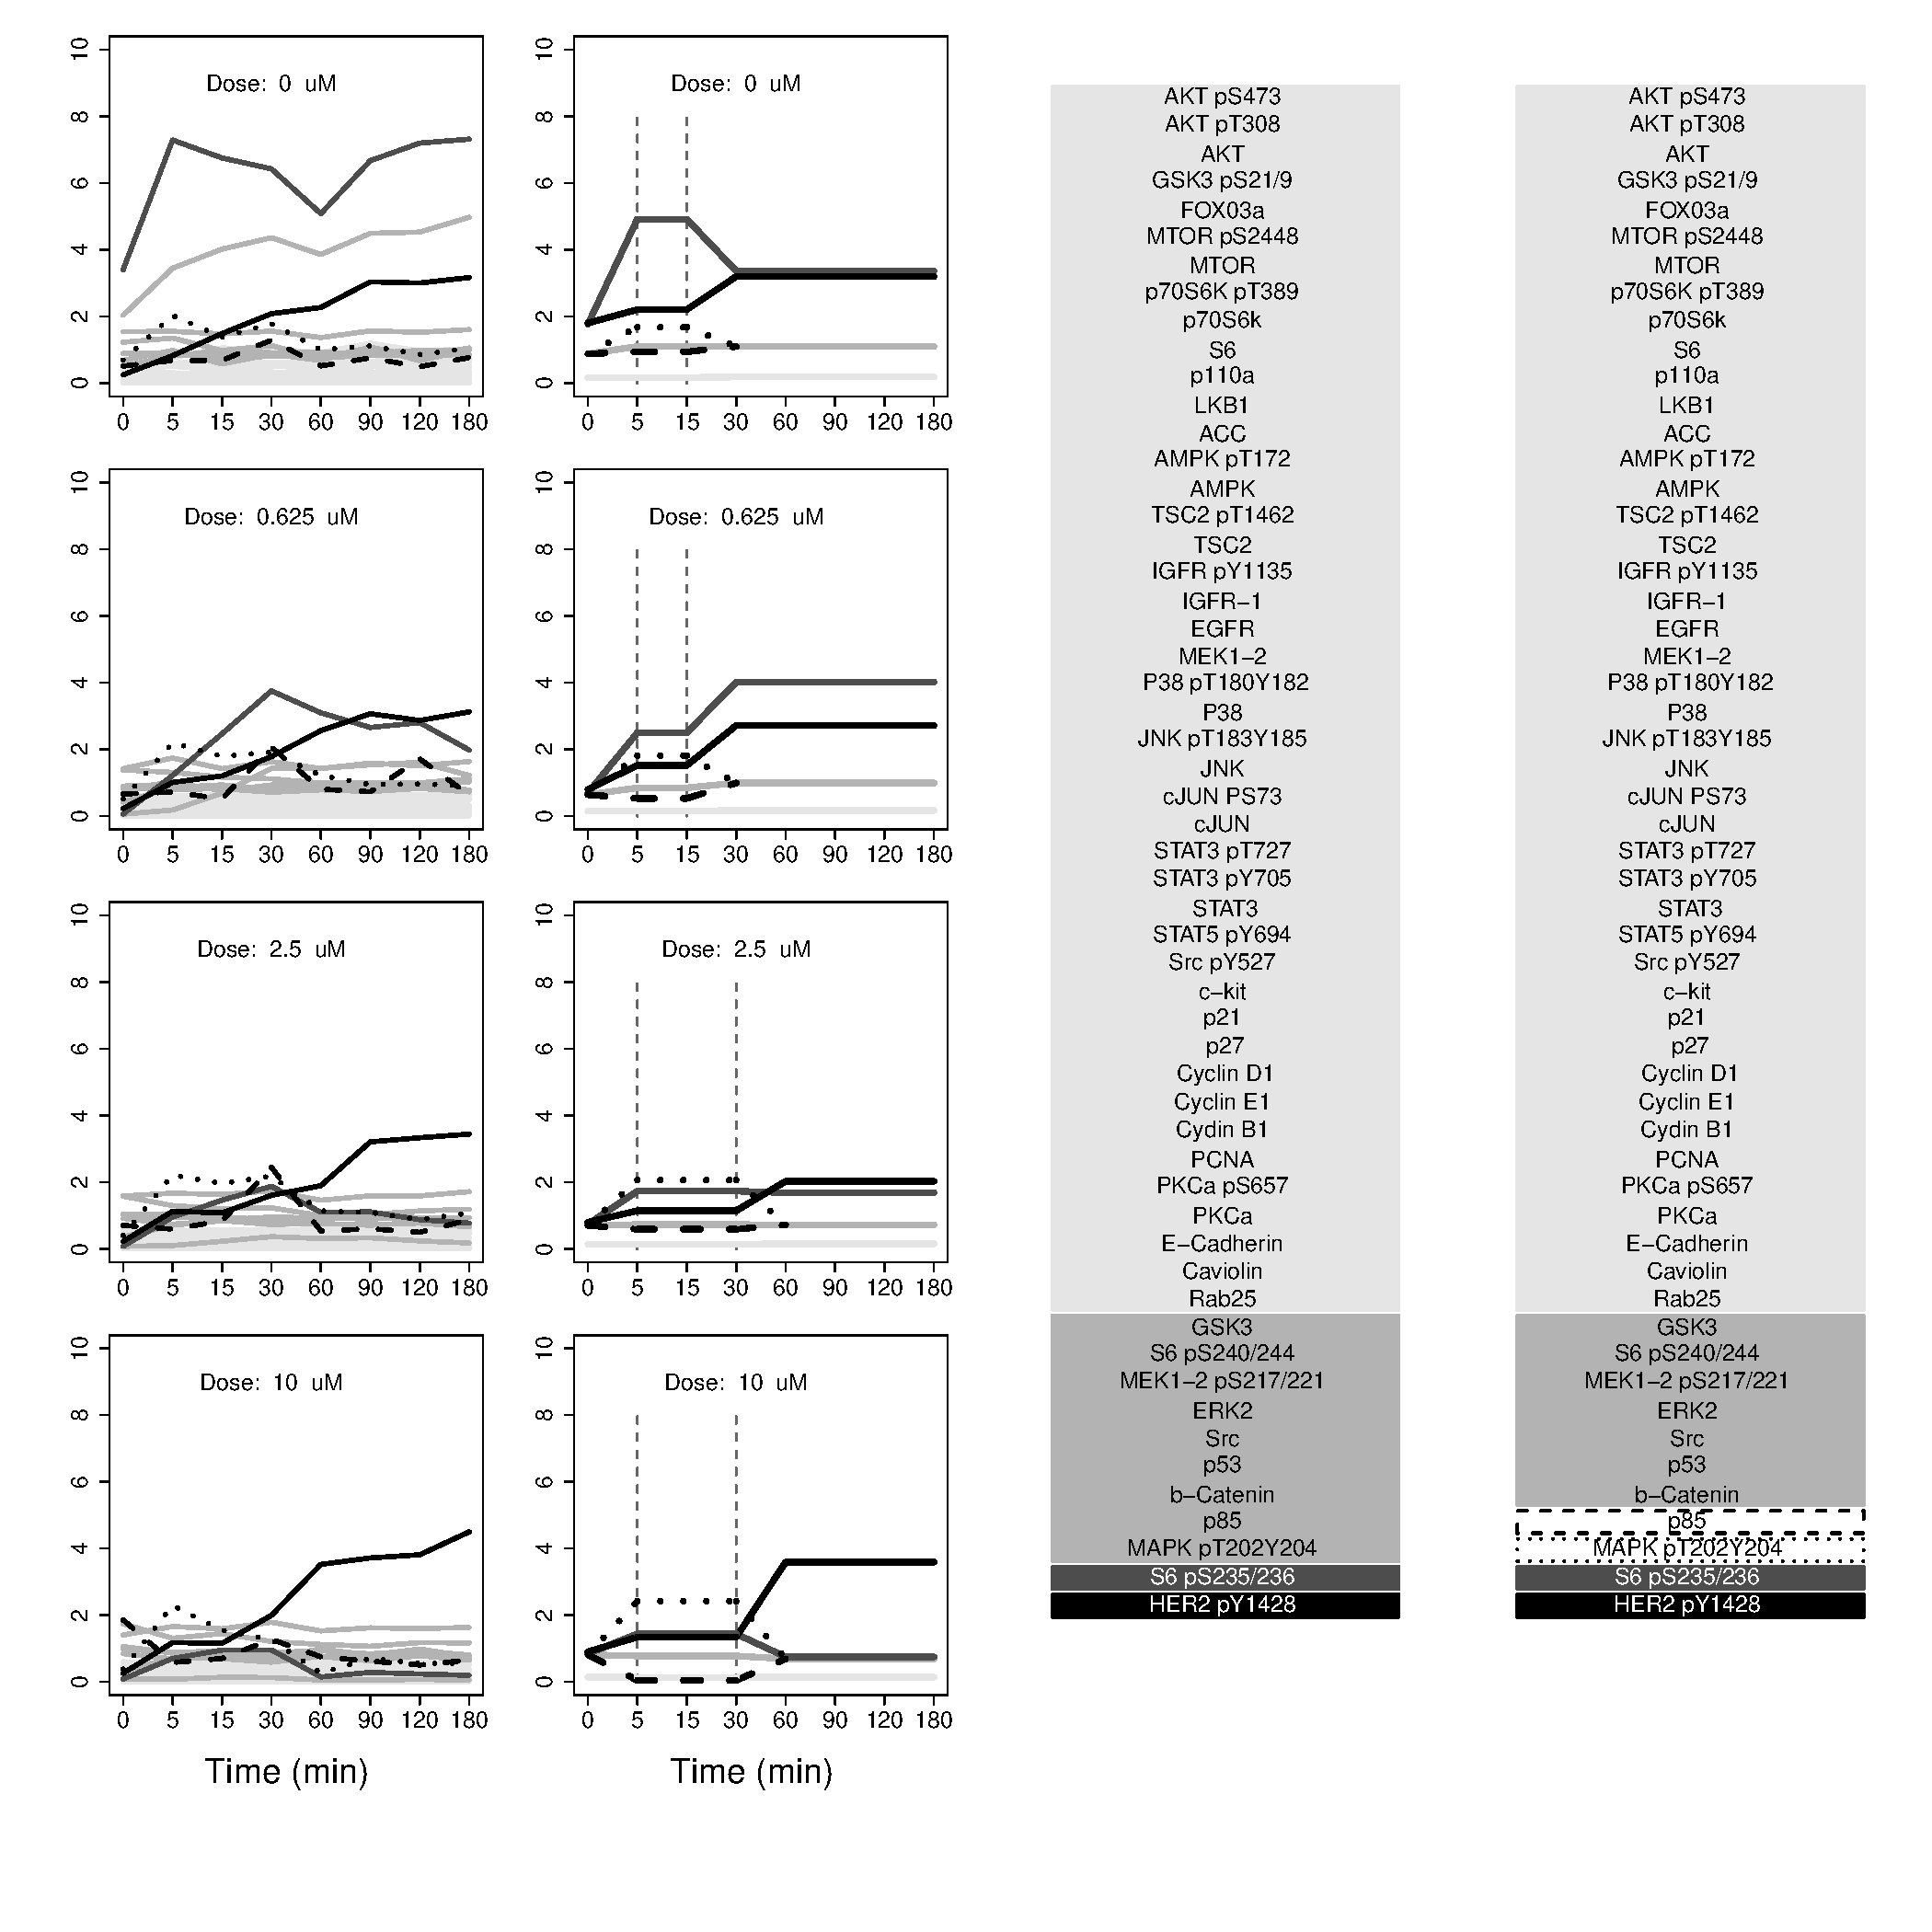
\includegraphics[scale=0.4]{figs_biometrics/results_cc_1_d_1_gray.pdf}\\[-.2cm]
%\phantom{x}{\footnotesize \hspace{1.75cm} TIME}
\caption{Results for proteins in cell line $c=1$ exposed to PI3K inhibitor ($d=1$). Colors (grayscale) denote distinct clusters with dashed lines corresponding to additional clusters formed at refinement.
  Columns 1 and 2 show $\ybar_{it}$ and $\mu_{i\ell t}$ as in
  Figure \ref{fig:mean_curves_simulation}. The horizontal axis contains the observed times
  measured in minutes.
  Columns 3 and 4 show the original partition before refinement
  ($\bfdelta^1_{cd}$, column 3) and
  the refined partition after refinement ($\bfdelta^2_{cd}$, column 4).}
%\note{ {\bf C:} was
 % ``Third
 % column: list of proteins colored by the cluster it belongs to before
 % coagulation and after refinement. Fourth column: same, but with colors
 % corresponding to clusters after coagulation and before refinement.''\\
 % But the 4th column has 2 more clusters, must be the refined partition?}
\label{fig:result_c1_d1}
\end{figure}


\begin{figure}[tbp]
\phantom{xx} 
\hskip 2cm $\ybar_{it}$ by $\hat{\delta}$  \hspace{0.8cm} $E(\mu^*_{\ell t}(m)\mid y, \hat{\delta})$
  \hspace{0.9cm} coagulation \hspace{0.9cm} refinement\\
    \rotatebox{90}{\hspace{2cm} dose $\ell=3$ \hspace{1.5cm}
                               $\ell=2$ \hspace{2cm}
                               $\ell=1$ \hspace{2cm}
                               $\ell=0$                             }
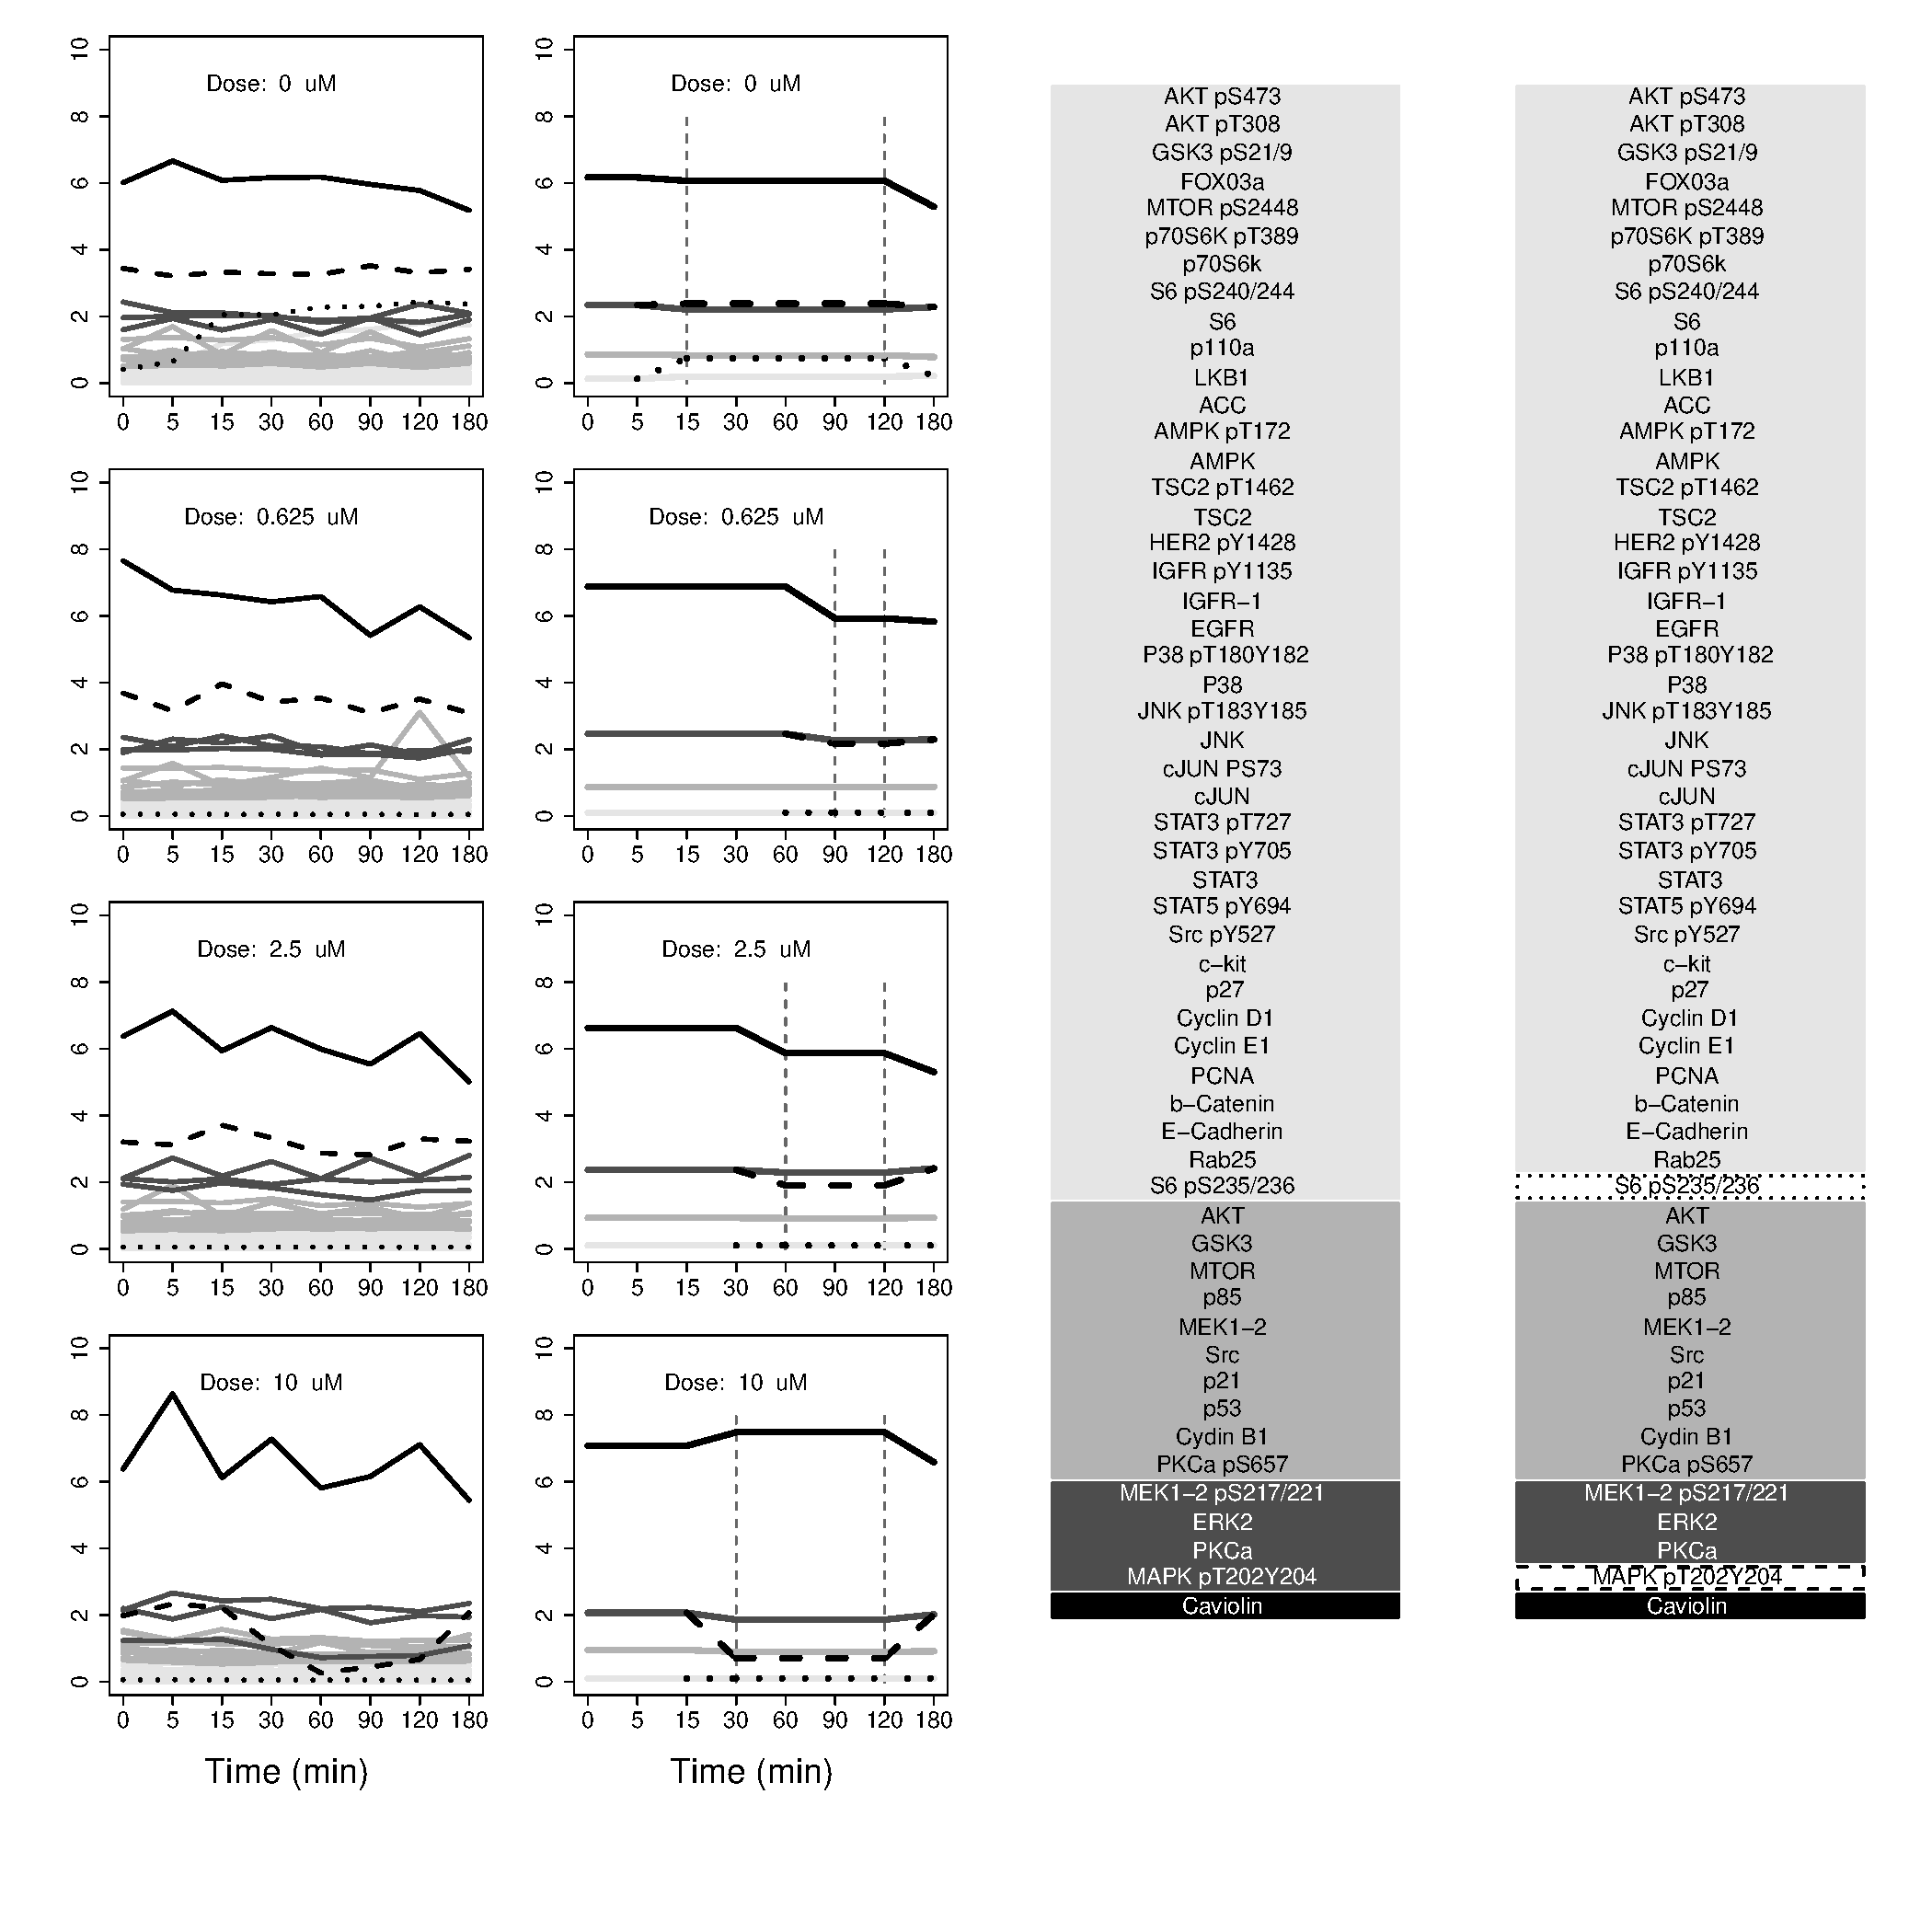
\includegraphics[scale=0.4]{figs_biometrics/results_cc_2_d_1_gray.pdf}\\[-.5cm]
%\phantom{x}{\footnotesize \hspace{1.75cm} TIME}
\caption{
Same as Figure \ref{fig:result_c1_d1}, now for cell line $c=2$.}
\label{fig:result_c2_d1}
\end{figure}


Additionally, in Figure \ref{fig:eda} we illustrate the benefit of the
time-dependent clustering, with only two change points when the
partition changes.
In the figure we explore the use of independent clustering at each
time point, using k-means for an easy implementation.
While one could still identify a small number of proteins that seem
to have their expression gradually increased or decreased at higher
doses of the PI3K inhibitor, there is substantially more noise in the
summary than in the corresponding plot in Figures
\ref{fig:result_c1_d1} and \ref{fig:result_c2_d1}.


\begin{figure}[tbp]
\centering
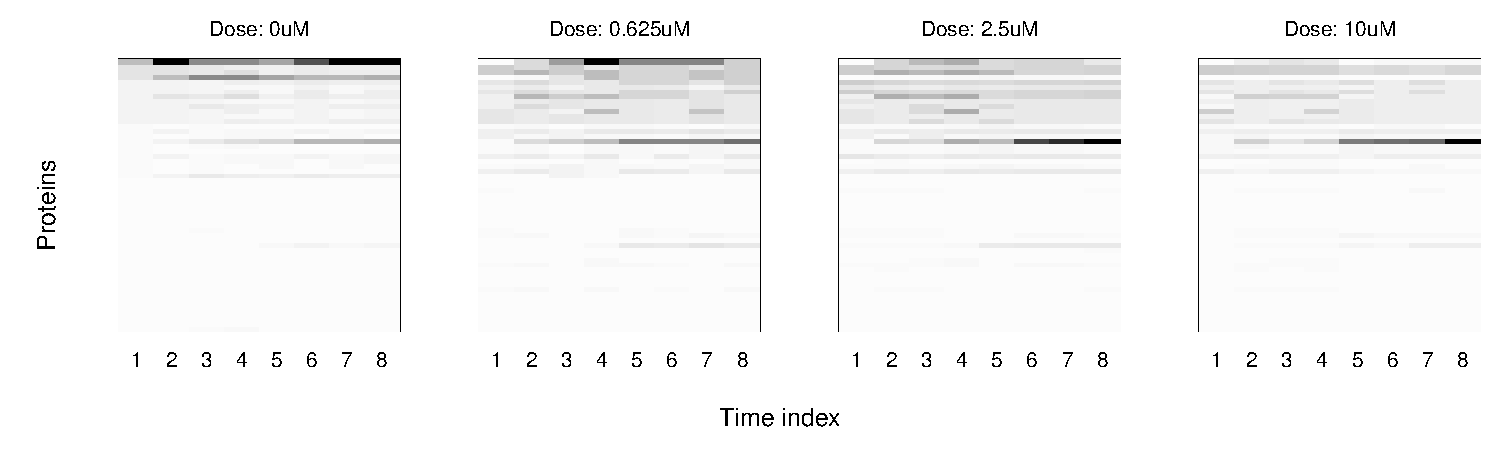
\includegraphics[scale=0.55]{figs_supporting_info/SuppInfo_ea_partition_times_11}
%\includegraphics[scale=0.6]{newfigs/ea_partition_times_11}
\caption{Independent k-means (k=5) estimation of partitions across time for different doses of PI3K inhibitor administered to cell line 1. For a fixed column (time index), each color represents the estimated cluster specific mean for that particular protein (higher expressions are darker).}
\label{fig:eda}
\end{figure}


% shows a preliminary estimation of the partitions
% carried out by k-means indepently across time. This approach is not
% capable of sharing information across time and as a result the cluster
% configurations exhibit wide variation for consecutive times that is
% likely to be simply random noise. 

\section{Discussion}
We introduced a model for finding a subpopulation of proteins that are
most affected by a particular intervention. The key element of the
model is a sequence of random partitions subject to the desired
monotonicity. The same inference -- without any change in the
probability model -- can be interpreted as inference on
% a change point in
mean protein expression over time, with the clusters serving
the purpose of adaptively borrowing strength across proteins, doses,
drugs and cell lines. The latter happens only at the level of
hyperparameters.  The approach is meaningful in any inference problem
with a sequence of partitions that include a notion of
monotonicity. It is most appropriate when limited data or high
noise leaves more complexly structured models impractical to fit.

Several extensions and generalizations of the proposed model are
possible. With more data one could replace the piecewise constant
mean response by a piecewise linear mean response with little change
in the remaining model. In the application to the RPPA data it was
reasonable to assume that once the treatment effect wears off the mean
response would revert to the initial levels. Other applications might
call for lasting treatment effects, allowing for a different final
level. Also, in other applications the use of more than two change
points might be meaningful, with possibly different sequences of
refinements and coagulations.

In the discussion following equation \eqref{eq:lik} we commented on alternative priors on $\Sigma_c$. In an application with richer data one could alternatively consider a Gaussian Process prior with more general covariance structure.

The main limitation is the computationally awkward problem of estimating
the size of the partitions. With respect to the application, a limitation
is that the described inference targets only mean expression levels,
missing changes that are in the dependence structure. The latter is
plausible when the intervention affects pathways and feedback mechanisms.


\chapter{Dependent Mixtures: Modelling Cell Lineages}
\label{ch:cell_lineage}
\index{Instructions for Preparing Dissertations, Theses, and Reports%
@\emph{Instructions for Preparing Dissertations, Theses, and Reports}}%


\section{Introduction}

This chapter introduces a Bayesian mixture model with dependent prior on the
component-specific parameters.
The simplest Bayesian mixture models assume independent
priors on cluster-specific parameters that index the sampling model
for each term of the mixture model, motivated mostly by ease of implementation.
For a review of Bayesian inference in mixture models see, for example, \citet{fruhwirth2006finite} and \citet[Chapter 1]{handbookmixtures2019}. 

However, in many situations, the observed data structure is not well supported by independent mixture components.
\citet{xu2016bayesian} argue for priors that favor diverse and parsimonious components in the mixture via determinantal point process. 
The idea is to favor mixture models with terms that define meaningfully different subpopulations. 
This becomes important if the inference aim is related to a biological interpretation of the underlying structure. 
While one can argue that asymptotically posterior inference in mixtures will concentrate on a parsimonious structure \citep{rousseau2011asymptotic}, this is not true for any finite sample size unless appropriate model assumptions are explicitly introduced.
In this paper we consider an inference problem that gives rise to a special type of parsimony in a mixture model.


\subsection{Modeling cell lineage data}
\label{sec:intro_cell_lineage}
The work developed in this chapter is motivated by the study of cell lineages. Cell lineage data comes from single-cell transcriptomics and it is used to recover the evolutionary path of cells in a given environment.
The finer resolution of single-cell assays such as single cell RNA sequencing experiments (scRNAseq) in comparison with aggregated "bulk" data provides cell-specific data. Applications include for example studies in immune systems \citep{stubbington2017single,miragaia2017single}, virus-host interactions \citep{cristinelli2018use}, hematopoiesis \citep{wilson2018single,dharampuriya2017tracking} among others. 
In particular, single-cell assays allow to trace back the ``history'' of fully differentiated cells starting from their precursors, so they have become very important to the study of cell lineages \citep{stubbington2017single}.

A typical cell lineage dataset contains a sample of cells from a certain tissue along with cell-specific transcriptional profiles obtained, for example, from scRNAseq. 
Such profiles exhibit differences that are associated with the development stage of the cell. 
For instance, stem cells evolve into fully differentiated cells according to a process characterized by gradual transcriptional changes. Therefore, important differences are observed in transcription profiles along the development path of the cell. 
Another potential application concerns temporal transformation of the cells, e.g. during cancer progression. 
Lineage inference is then carried out to identify the underlying path of development from the initial state of the cell until its matured states. 
For a more detailed description of the objectives and challenges of lineage inference, see \cite{korthauer2016statistical} .


%\begin{figure}[!ht]
%	\centering
%	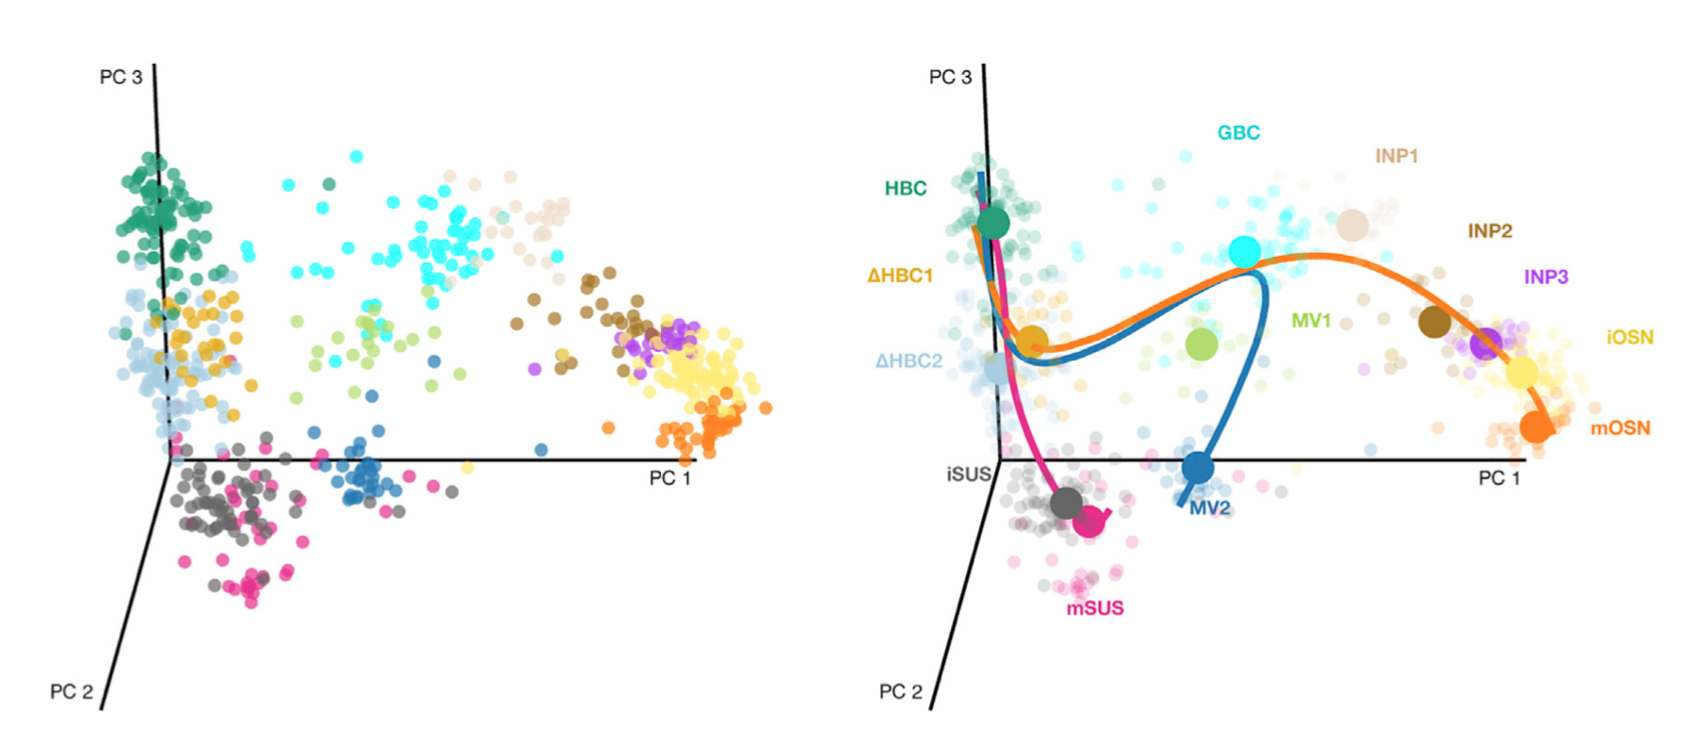
\includegraphics[width=.85\linewidth]{./Img/sample_data}
%	\caption{Left panel: Three-dimensional representation of single-cell gene expression profiles based on principal component analysis (data of \cite{fletcher2017deconstructing}); cells are colored by cluster. Right panel: results using the ``Slingshot'' method of \cite{street2018}.}
%	\label{fig:ex_data}
%\end{figure}


\begin{figure}[!ht]
	\centering
	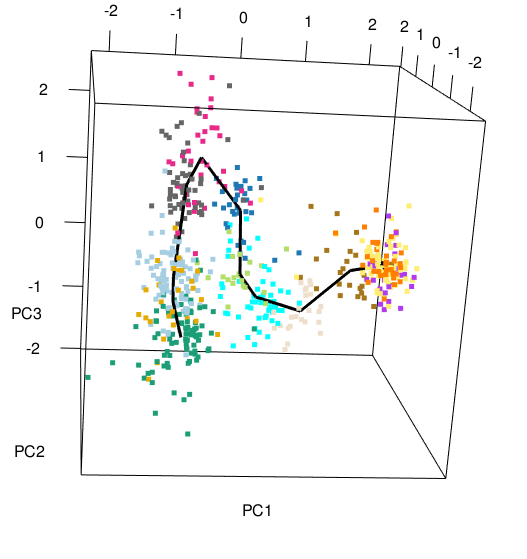
\includegraphics[width=.4\linewidth]{./Img/fletcher/fletcher_data_3d.png}
	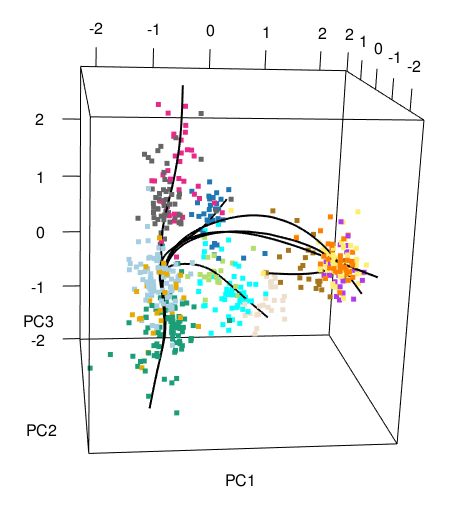
\includegraphics[width=.4\linewidth]{./Img/fletcher/fletcher_data_slingshot.png}	
	\caption{Left panel: Three-dimensional representation of single-cell gene expression profiles based on principal component analysis (data of \cite{fletcher2017deconstructing}); cells are colored by cluster. Right panel: results using the ``Slingshot'' method of \cite{street2018}.}
	\label{fig:ex_data}
\end{figure}

Typically, the process of estimating the latent tree in cell lineage problems is done in three sequential steps. First,  dimension reduction methods are applied to summarize information from the high dimensional scRNAseq data; then clustering of the cells is carried out in the reduced dimensional space; finally, the latent tree is inferred given the estimates of the partition of cells. Figure \ref{fig:ex_data} illustrates the results of this sequential approach applied to a lineage cell lineage dataset. Notice how in Figure Figure \ref{fig:ex_data} (and the following discussion) the data includes observations on all nodes of the tree, not only the leaves. This is because the data is a snapshot of cells accross all intermediate steps in the evolution of the cells.

\cite{Shiffman18} introduce a generative model based on a Dirichlet diffusion process \citep{neal:03}. 
This model, however, despite introducing a notion of tree along which cell evolution occurs, the model does not favor simple trees with well dinstinguished clusters of cell. Trees from a Dirichlet diffusion process are generated on a latent space via Brownian motion and thus do not enforce neither a partition nor a parsimonious representation of the data. 

In contrast, \cite{street2018} develop a method (``Slingshot'') that takes as input a partition of the cell lines into different cell types and returns a smooth version of the underlying MST defined by the clusters' centroids: the paths from root to leaves are smoothed by principal curves. The Slingshot procedure requires observations to be clustered, which is done sequentially by a k-means algorithm for instance, before the construction of a minimum spanning tree on the cluster centroids. Such sequential approach (of first fixing the partition of cells, then using the centroids as nodes of the MST) is very common in the bioinformatics literature despite its assumption that the lineage structure (represented by the MST) does not play a role in clustering the cells. Such assumption is not biologically ideal.


In the following section we propose an inference approach that uses a model-based Bayesian perspective such as in \cite{Shiffman18}, but in the context of mixtures as in ``Slingshot''.
That is, we propose a Bayesian dependent mixture model for cell lineage inference. 
The mixture components represent clusters of cells in the same development stage and the dependence is defined by a latent random tree with nodes that correspond to the centroid of the clusters. The cluster and lineage structures are modeled jointly and as a consequence, the lineage represented by the random tree structure is allowed to affect the clustering of cells. 
Full posterior inference on the clusters, the random tree and pseudotimes are obtained by Markov chain Monte Carlo (MCMC). 


\subsection{Dependent mixture models}

The proposed model is a variation of Bayesian mixture models in which dependent priors are assumed. 
Clusters of cells should be dependent on each other due to the fact that mixture components represent distinct intermediate states in the continuous process of cell development. 
Most literature on Bayesian mixture models assumes a priori independent cluster-specific parameters, with some exceptions. 
\cite{xu2016bayesian} describe the application of determinantal point processes (DPP) \citep{dpp_original} in Bayesian mixture models as a way to impose repulsive stochastic behaviour for the prior on the mixture components. 
The motivation comes from the observation that similar mixture components do not make the model more flexible. 
Conversely, they only create redundancy and hurt the interpretability of the components. 
In the context of cell lineage data, the repulsive nature of the DPP would enforce the intermediate states of cell development to be dissimilar from each other.

Another motivation for dependent mixtures is the sharing of information between the different groups, causing a shrinkage effect that is also a form of regularization. 
Mixed effect models is a key example of the use of hyperpriors for regularization \citep{lindstrom1990nonlinear,alston2012bayesian,lachos2013bayesian}.
In Bayesian non-parametrics, hierarchical Dirichlet processes \citep{HDP} incorporate shrinkage effect by assuming dependent component-specific Dirichlet processes (DP) $G_j \sim DP(\alpha_0, G_0)$ for mixture components $j=1, \dots, K$ with a common base measure $G_0$ that is itself a DP. 
Since DPs generate discrete random measures with the countably infinite support consisting of an iid sample from the base measure, it follows from the discreteness of $G_0$ that all $G_j, \ j=1, \cdots, K$ will all share the same atoms.


An application of mixture models with predictor-dependent components is described in \cite{chung2011local}. 
The authors define a Dirichlet process that assigns stick-breaking weights and atoms to random locations in predictor space, therefore obtaining random probability measures (which define the distribution of the mixture components) indexed by covariates in a continuous way.
 

Our proposal is to define dependence on the components of the mixture in a way that explicitly incorporates the biological structure that characterizes cell lineage applications. 
We therefore propose the use of a random tree structure not only to explain the snapshot in the latent space of the continuous development of cells from its initial stage into mature differentiated cells, but also to model the dependence structure between the clusters of cells.
Regularization is incorporated in the form of a penalization on trees with too many nodes or with redundant edges. 
Our proposed model builds upon the slingshot model in \cite{street2018} in which a Minimum Spanning Tree is calculated given the estimated centroids of the clusters of cells in a latent low dimensional space. The authors then use projections onto the MST to get a point estimate of the pseudotimes for each cell. 
In contrast, by formally constructing a Bayesian mixture model with random trees on such latent space, we are able to provide full inference (with uncertainty captured by the posterior samples obtained through MCMC) on the clusters of cells, on the underlying tree structure and also on pseudotimes. In addition, the model assumes the partition of cells to depend on the lineage structure.

\section{Dependent  Mixture Models for Cell Lineage Data}


% \subsection{A Dependent Mixture Model}
Let $\bfy_i \in \mathbb{R}^D$ denote the recorded markers for the $i$th cell. 
In a study of cell lineage, the raw data could be biomarkers, i.e., protein levels for some selected proteins. 
The raw data are typically further processed by extracting, for example, the first few principal components which become the data $\bfy_i$ in the upcoming discussion.

We start the construction of a Bayesian inference model by assuming a mixture sampling model for $\bfy_i$, $i=1, \ldots, n$. 
Let $\bftheta$ denote all unknown parameters. 
We assume
\begin{equation}
	  \bfy_i \mid \bftheta \iid \sum_{j=0}^k w_j \ N(\bfy_i  \mid \bfmu_j, \Sigma_j).
	\label{eq:likelihood}
\end{equation}
The parameter vector $\th$ includes, in particular, the number of terms in the mixture, $k+1$, the location parameters $\bfmu_j$ and the covariance parameters for each cluster in the mixture model, and the relative weights $w_j$, $j=0, \ldots, k$.

In words, we assume a mixture of normals for the data $\bfy_i$, including cluster-specific covariance matrices $\Sigma_j$ and cluster-specific location parameters $\bfmu_j$.
Next, we introduce a dependent prior across $\bfmu_j$.
Dependence is supported by the nature of the cell subpopulations being biologically related as part of the cell differentiation process.


 Recall that the goal is  to infer a structure that reflects the cell evolution path and its possible branching,  starting with an original cell population indexed by $k=0$ (and biologically known to be the root population).
 We represent this cell evolution path as a tree that includes the terms $\bfmu_j$ in the mixture model \eqref{eq:likelihood} as the vertices, which are connected by edges that represent the cell differentiation.
An additional set $\bfb=(b_1, \ldots, b_k)$ of indicator variables $b_j \in \{0,\ldots,k\}$ records the tree structure by specifying for each node the index of the parent node. The root node, $j=0$ has no parent.
A prior on the tree implicitly defines the prior probability model for the mixture component locations $\bfmu_j$, as described in Sections \ref{sec:soft_mst} and \ref{sec:model2_mst}. 

In order to define a meaningful notion of cell evolution, we need to carefully choose the form of such tree.
This is achieved by defining a tree with a globally-dependent structure, which is able to induce repulsions between the branches and to avoid redundant components. 
For example, we avoid the possibility of a tree to grow back into itself. 
In fact, cell evolution follows a ``monotonicity'' requirement in the sense that cell characteristics evolve towards progressive degrees of differentiation, not going back to an undifferentiated stage.

 We introduce a preference for such structure using the notion of a minimum spanning tree (MST), whose origin traces back to \cite{boruuvka1926contribution}.
A MST is an edge-weighted, undirected graph that connects all vertices together, without any cycles and with the minimum possible total edge weight.  
The weight on an edge is  the distance between the two nodes of the corresponding edge. 
In such a way, the most likely tree induces the desired parsimony requirement. 
In fact, given a set of nodes representing the different cell subpopulations, a MST can be seen as the most parsimonious way to represent the cell lineage.


We consider two alternative priors for $(k,\bfmu_1,\ldots,\bfmu_k)$ based on a MST.
One model is centered around trees that constitute a MST of the locations $\bfmu_j$, but also allows trees that are not MST. 
The second model restricts the tree to be a MST, making $\bfb$ a deterministic function of $(\bfmu_0,\ldots,\bfmu_k)$.


\subsection{Soft MST-dependent prior}
% Mixture model of soft Minimum Spanning Trees
\label{sec:soft_mst}


Let $\mathcal{T}_k = (k, \bfmu_1, \dots, \bfmu_k, b_1, \dots, b_{k})$
denote the tree, including cluster locations $\bfmu_j$ (note that $\bfmu_0$ is known and hence no prior is assigned to it) and tree
structure $\bfb$.
The soft-MST (s-MST) prior defines a dependent prior on the cluster
locations as 
\begin{equation}
  p(\bfmu_1, \dots, \bfmu_k, \bfb, k) \propto \prod_{j=1}^k
  \left\{ q(\bfmu_j) \right\} \exp\left\{- \alpha \sum_{j=1}^k
    d^2(\bfmu_j, \bfmu_{b_j}) \right\} q(k).
\label{eq:prior1}
\end{equation}
with $\bfb$ restricted to tree structures, i.e., no cycles and a single known root in $\bfmu_0$. Also, notice that \eqref{eq:prior1} includes $k$ as a random variable.

In equation \eqref{eq:prior1}, $d(\bfmu_i, \bfmu_j)$ denotes the Euclidean distance between two nodes $\bfmu_i$ and $\bfmu_j$. The terms $q(k)$ and $q(\bfmu_j)$ are reference probability models. We use $q(\bfmu_j)\sim N(\bfmu_j \mid m_0, \sigma^2_0 I)$ where $I$ denotes the identity matrix of dimension $D$. The penalty parameter $\alpha$ controls the level of shrinkage towards a MST, with $\alpha=0$ implying no shrinkage and $\alpha \rightarrow \infty$ implying a deterministic restriction to MSTs. In summary, equation \eqref{eq:prior1} is the prior on the random tree. It is difficult to visualize $p(\mathcal{T}_k)$ by way of prior simulation.

It is important to notice that $q(k)$ and $q(\bfmu_j)$ are not the marginal models for $k$ and $\bfmu_j$. The marginal distributions are implicitly determined by $q(k)$, $q(\bfmu_j)$ and by the parameter $\alpha$. In fact, conditionally on $k$, the model in \eqref{eq:prior1} reduces to 
$$
p(\bfmu_1, \dots, \bfmu_k, \bfb | k) = \frac{1}{Z_{k}}
\prod_{j=1}^k \left\{ q(\bfmu_j) \right\} \exp\left\{- \alpha
  \sum_{j=1}^k d^2(\bfmu_j, \bfmu_{b_j}) \right\},
$$
where
$$
Z_{k} = \int \dots \int_{\mathbb{R}^{p \times k}} \prod_{j=1}^k \left\{
  q(\bfmu_j)\right\} \cdot \left[ \sum_{b_1=0}^k \dots
  \sum_{b_k=0}^k \exp\left\{- \alpha \sum_{j=1}^k d^2(\bfmu_j,
    \bfmu_{b_j}) \right\} \right] \ d\bfmu_1 \dots  d\bfmu_k
$$
is an intractable normalizing constant. The marginal prior on $k$ can
be written as $ p(k) \propto Z_{k} \ q(k)$ with normalization constant $\sum^{\infty}_{k=1} Z_{k} \ q(k)$. It is easy to see that $p(\bfmu_1, \dots, \bfmu_k, \bfb, k)$
defined in \eqref{eq:prior1} is proper (see Appendix
\ref{sec:proper_prior}).

The dependence among the centers is induced by the exponential term,
that penalizes complex branching structures; for example, in trees
with too many nodes or with redundant edges. Therefore, the prior can
be seen as a regularization term, that is ballanced by the
likelihood, which tends to favor complex trees that provide better
fit to the training data. The parameter $\alpha$ determines the
strength of the regularization implied by the prior in comparison with
the likelihood of the data. Implicit in \eqref{eq:prior1} is the fact
that the only branching structures $\bfb$ allowed are the ones that
span trees with no internal cycles.
% Notice that complex branching structures are allowed (albeit
% discouraged, unless the data suggest so), not restricting to the
% case of binary branching. 

%The dependency among the centers is induced by the exponential term,
%that penalizes branching structures that are redundant and not
%supported by the data.  
%Implicit in \eqref{eq:prior1} is the fact that the only branching
%structures $\bfb$ allowed are the ones that span a tree with
%vertices $\bfmu_1, \ldots, \bfmu_k$ having no cycles. Notice that
%complex branching structures are allowed (albeit discouraged, unless
%the data suggest so), not restricting to the case of binary
%branching. 

This joint prior, despite presenting an intractable normalizing
constant, induces simple conditionals. For example, note that  
\begin{multline}
  p(b_j = i | \bfmu_1, \dots, \bfmu_k, \bfb^{(-j)},  k)
  \propto \exp \left\{ - \alpha \ d^2(\bfmu_j, \bfmu_i) \right\},
  \\ \forall i = 0, \dots, k ,\ \forall j = 1, \dots, k 
  \label{eq:b_cond}
\end{multline}
and that 
\begin{equation}
  p(\bfmu_j | \bfmu^{(-j)}, \bfb, k) \propto q(\bfmu_j) \exp
  \left[ - \alpha \left\{ d^2(\bfmu_j, \bfmu_{b_j}) + \sum_{l : b_l
        = j} d^2(\bfmu_l, \bfmu_j) \right\} \right]. 
  \label{eq:mu_cond}
\end{equation}
Equations \eqref{eq:b_cond} and \eqref{eq:mu_cond} reflect the repulsive
effect of the prior on the branching structure.  In fact, the
conditional distribution for $\bfb$ favours minimum spanning trees
by assigning smaller probabilities to redundant structures,
e.g. branches that grow back.  This can be seen by the fact that each
branch is selected to be the shortest (with larger probabilities)
among those who preserve the spanning structure of the tree.  In the
case $\alpha \rightarrow +\infty$, this procedure has several
analogies with Prim's algorithm \citep[see][]{prim1957shortest}.  In
the opposite case, i.e. when $\alpha \rightarrow 0$, the prior on the
trees is invariant with respect to the branching structure and the
centers are independent.  The model in this case corresponds to a
finite mixture model with a prior on the number of components.  In
general, the model does a soft assignment of the branches to a MST
structure (s-MST).

The conditional prior on the means, instead has a different effect.
Each center is drawn from a linear combination of the independent
prior term and the position of its parent and children.  The larger
the $\alpha$ parameter, the more evident the attraction towards the
barycentre of parent and children.  Moreover, note that if the
distance $d$ chosen is the squared euclidean, the conditional
distribution of each $\bfmu_j$ is still normal, with updated
parameters, i.e.
\begin{align}
\bfmu_j | \bfmu^{(-j)}, \bfb, k &\sim \mathcal{N}\left( \bfmu_p, \Sigma_p\right),\nonumber \\ 
\bfmu_p &= \frac{\bm{m}_0/\sigma_0^2 + 2 \alpha (\bfmu_{b_j} + \sum_{l:b_l = j} \bfmu_l)}{1/\sigma_0^2 + 2 \alpha (1 + f_j)} \label{eq:mu_cond_eucl1} \\
\Sigma_p &= \left\{ \frac{1}{\sigma_0^2} + 2 \alpha (1 + f_j) \right\}^{-1} I.
\label{eq:mu_cond_eucl2}
\end{align}
where $f_j$ is the number of children of node $j$ and $(\bm{m}_0, \sigma_0^2)$ are the prior hyperparameters of $q(\bfmu_j)$. The Gaussian prior on $(\bfmu_j | \bfmu^{(-j)}, \bfb, k)$ is a fundamental feature that will imply posterior conditional conjugacy. 

For the weights and the kernel covariance we use conditionally conjugate priors, 
\begin{eqnarray}
	\Sigma_0, \dots, \Sigma_k & \sim & \IW\left( \nu, \Psi \right) \nonumber \\
	(w_0, \dots, w_k) \mid k &  \sim & \Dir(\delta, \dots, \delta) 	\label{eq:prior_cov}\\
	\alpha &\sim & \mbox{Exp}(\lambda_0) \nonumber\\
	k &\sim & \text{Geom}(k - 2 | r_0), \ k \geq 2. \nonumber
\end{eqnarray}


\subsection{Hard MST-dependent mixture model}
\label{sec:model2_mst}

% A special case of the model described in section \ref{sec:soft_mst} is
% obtained when the branches $b_j$ determine the minimum spanning tree
% with vertices $\bfmu_1, \ldots, \bfmu_k$. The MST structure is
% favoured when $\alpha \rightarrow +\infty$, although there is always a
% positive probability of sampling oher trees that are not the MST. In
% this section we show how a simple modification of the model described
% in section \ref{sec:soft_mst} can impose MST structure. We highlight
% that the resulting model is simpler to implement as it does not
% require sampling the branches $b_j$ while maintaining full
% conditionals in analitical form. The obvious drawback is the loss of
% flexibility in the branching structure. 

%(When should one prefer to enforce MST? )
The prior in \eqref{eq:prior1} formalizes a preference for parsimonious structure by favoring mixture models with clusters that are connected by a tree with short cumulative length. 
By favoring shorter cumulative length the model shrinks the tree structure towards a MST, but stops short of insisting on the tree actually being a MST. 
The model defines a joint prior $p(\bfmu,\bfb)$ on the cluster locations $\bfmu=(\bfmu_j)^k_{j=1}$ and the tree $\bfb$.
An alternative model, named here as hard-MST (h-MST), defines a prior on $\bfmu$ only and implies $\bfb$ by introducing the MST as a deterministic function $\bfb = \mbox{MST}(\bfmu)$ of $\bfmu$: 

\begin{equation}
  p(\bfmu_1, \ldots, \bfmu_k \mid k) \propto \prod_{j=1}^k
  \left\{ N(\bfmu_j; \ \bfm, \ \sigma^2_0I) \right\} \exp\left[ -\alpha
    \mathcal{W}\left\{ MST(\bfmu_1, \ldots, \bfmu_k) \right\} \right].
\label{eq:hMST}
\end{equation}

The term $\mbox{MST}(\bfmu_1, \ldots, \bfmu_k)$ in equation \eqref{eq:hMST} represents the minimum spanning tree with nodes $\bfmu_1, \ldots, \bfmu_k$ and edges $E_{\bfmu_1, \ldots, \bfmu_k} \subset \{1, \ldots, k\}^2$. The function $\mathcal{W}$ denotes the total length of a graph, which is defined by the sum of the squared lengths of its edges. Therefore, we have

$$\mathcal{W}(MST(\bfmu_1, \ldots, \bfmu_k)) = \sum_{(j_1, j_2) \in E_{\bfmu_1, \ldots, \bfmu_k}} d^2(\bfmu_{j1}, \bfmu_{j2}).$$

By taking the lengths of the edges squared to define the length of the whole tree, we preserve conjugacy for the component specific means. By enforcing the MST structure the h-MST model provides stronger parsimony (in terms of favoring simpler tree structures) if compared with the s-MST. The parameter $\alpha$ regulates the strength of influence of the MST on the clustering structure: the higher its value, the simpler the underlying tree structure due to a stronger penalization on the length of the MST.

Under the h-MST, the priors for the remaining parameters are the same as described in section \ref{sec:soft_mst} equation \eqref{eq:prior_cov} for the s-MST. 

As mentioned in subsection \ref{sec:intro_cell_lineage}, there is a crucial difference between our modeling approach and the two-step slingshot algorithm of \cite{street2018} with regards to the dependence relationship of the cell lineage and the cluster centroids. Although the hard MST-dependent mixture model defines the MST as a deterministic function of the cluster centers, it implies a regularization effect of the tree structure on the distribution of the centroids by favoring cluster-specific means that lead to simpler (shorter) MSTs. On the other hand, the clustering step in \cite{street2018} does not make use of the underlying lineage structure represented by the MST.

All full conditional distributions for this model are analytically available, except for $p(\bfmu_j\mid \bfy, \mbox{rest})$ for which a Mtropolis-Hastings step was implemented. More details are available in Appendix \ref{sec:app_hmst}.



\section{Posterior Inference}
\label{sec:mst_inference}

In this section, we present the posterior simulation scheme to infer the tree structure, the optimal clustering configuration, as well as the estimation of the pseudotimes for each cell. For both the s-MST and h-MST models, the inference procedure is done via reversible jumps MCMC. 


For inference with an unknown number of components $k$ we 
added a prior $k \sim \mbox{Geom}(k - 2 | r_0), \ k \geq 2$ and implement transdimensional  posterior simulation, to accommodate the variable dimension of the parameter vector as $k$ changes. The soft-MST prior uses reversible jump MCMC (RJ-MCMC) \citep{green1995}  to implement trans-dimensional transitions.  Proposing a tree also requires a proposal for the branching structure. However, given $k$ nodes the total number of spanning trees is $k^{k-2}$, implying a curse of dimensionality for even fairly moderate values of $k$.  This would in turn lead to inefficient proposals, which cause the algorithm to mix poorly.

In order to overcome this issue, we propose a variant of the RJ-MCMC
which has been previously used in \cite{xu2016bayesian} and
\cite{lee2015bayesian}.  Denote the parameters with
$\bm{\theta}_k = (\bfmu_1, \dots, \bfmu_k, b_1, \dots, b_k, w_0,
\dots, w_k, \Sigma_0, \dots, \Sigma_k)$.  In the RJ-MCMC, a proposal that involves a
change of $k$ to $\tilde{k}$ would require to propose also a new set
of parameters $\tilde{\bm{\theta}}_{\tilde{k}}$.  In practice, the
joint proposal for a ``new'' dimension and a ``new'' set of
parameters, decomposes in $q(\tilde{\bm{\theta}}_{\tilde{k}},
\tilde{k} | \bm{\theta}_{k}, k) = q(\tilde{\bm{\theta}}_{\tilde{k}} |
\tilde{k}, k, \bm{\theta}_{k})\ q(\tilde{k} | k)$. In practice, it is difficult to make good proposals $q(\tilde{\bftheta}_{\tilde{k}}, \tilde{k} \mid \bftheta_k, k)$ and $q(\bftheta_k, k \mid \tilde{\bftheta}_{\tilde{k}}, \tilde{k} )$ with reasonable acceptance probabilities. 

We follow an approach from \cite{lee2015bayesian} nd \cite{xu2016bayesian}.
The idea is to split the data into two parts: a small
training set $y^\prime$ that serves the purpose of creating
informative proposal distributions, and a test set $y^{\prime \prime}$
to evaluate the acceptance ratio.  Let $p_1(\bm{\theta}_k | y^\prime)
= p(\bm{\theta}_k | k, y^\prime)$ denote the posterior distribution
under $k$ using the training sample $y^\prime$.  We use $p_1$ in two
instances.  First, we replace the original prior term $p(\bm{\theta}_k
| k)$ and, second, we also use it as proposal distribution
$q(\tilde{\bm{\theta}}_{\tilde{k}} | \tilde{k})$.  The test data
$y^{\prime \prime}$ is then used to evaluate the acceptance
probability.  By the nature of the Metropolis-Hastings acceptance
probability the proposal distribution and the prior factor in the
target distribution cancel out, making this a feasible strategy, i.e.
\begin{align}
\alpha(\tilde{\theta}_{\tilde{k}}, \tilde{k}\mid \theta_k, k) &= \min \left\{ 1; \frac{p(\tilde{k}) \ p (y^{\prime \prime} | \tilde{\bm{\theta}}_{\tilde{k}}, \tilde{k}) \cancel{p_1(\tilde{\theta}_{\tilde{k}} \mid \tilde{k})}\ \bcancel{q(\theta_k | k)} q(k | \tilde{k}) }{p(k) \ p (y^{\prime \prime} | \bm{\theta}_k, k) \ \bcancel{p_1(\theta_k \mid k)} \ \cancel{q(\tilde{\theta}_{\tilde{k}} \mid \tilde{k})} \ q(\tilde{k} | k)} \right\} \nonumber \\
&=\min \left\{ 1; \frac{p(\tilde{k}) \ p (y^{\prime \prime} | \tilde{\bm{\theta}}_{\tilde{k}}, \tilde{k})\ q(k | \tilde{k})}{p(k) \ p (y^{\prime \prime} | \bm{\theta}_k, k) \ q(\tilde{k} | k)} \right\},
\label{eq:alpha}
\end{align}
The strategy has an analogy with model comparison via fractional Bayes factors \citep{o1995fractional}.


%\subsection{Inference under the s-MST Prior}
%\label{sec:post_inf_smst}

Performing inference for a fixed size tree is straightforward under the soft-MST.
In particular, the full conditionals are available in closed form and easy Gibbs sampling updates can be implemented (details are described in Appendix \ref{sec:app_smst}).

%\subsection{Inference under the h-MST Prior}
%\label{sec:post_inf_hmst}

Inference under the h-MST with fixed tree size is similar to s-MST. Full conditionals are also analytically available, except for the component-specific means $\bfmu_1, \ldots, \bfmu_k$, which are sampled according to a Metropolis-Hastings step. 

In summary, each full conditional $p(\bfmu_j \mid \bfmu^{(-j)}, \bfy, rest), \ j = 1, \ldots, k$ is a finite mixture of truncated normals with non-overlapping truncation regions which are hard to determine analytically. The issue of sampling from $p(\bfmu_j \mid \bfmu^{(-j)}, \bfy, rest)$ is avoided when approximating it by the efficient Metropolis-Hastings proposal 

\begin{multline*}
q(\tilde{\bfmu}_j \mid \bfy, \bfmu^{(-j)}) \propto \prod_{i\in S_j} N(\bfy_i; \tilde{\bfmu}_{j}, \Sigma) N(\tilde{\bfmu}_j; \bfm, \sigma^2_0I) \exp\left\{-\alpha\sum_{i \in V_j} d^2(\bfmu_i, \tilde{\bfmu}_j) \right\},
\end{multline*}

\noindent where $S_j = \{I: \ c_i = j\}$ and $V_j$ denotes the ser of neighbors of node $j$ in the current $MST(\bfmu)$. The proposal is built so that the acceptance probability equals 1 if the set of neighbors of $j$ in $MST(\tilde{\mu}_j, \mu^{(-j)})$ equals $V_j$. For further details, see Appendix \ref{sec:app_hmst}.

\subsection{Optimal partition}

Once the posterior distribution is obtained vvia MCMC, it is necessary to assign each observation to a cell subpopulation, which corresponds to a point estimate of the partition of cells a posteriori. Although the posterior includes also values for the visited partitions $\{\bm{c}^{(m)}\}_{m=1}^M$ where $m$ denotes the MCMC iterations, finding a point estimate for a random partition is non-trivial due to the cardinality of the space of partitions (Bell number). 
The posterior mode, for example, is not an adequate solution as each support point might have a negligible posterior probability.
In the Bayesian literature, a common approach is to use a decision theoretic framework.
In practice, one introduces a suitable loss function $L(\bm{c}_n,\hat{\bm{c}}_n)$ giving the cost of estimating the ``true'' $\bm{c}_n$ by $\hat{\bm{c}}_n$.
Then, a Bayes optimal estimate is given by any partition $\hat{\bm{c}}_n$ which minimizes the posterior expectation of the loss function. 
In other terms, the loss is averaged across all possible true clusterings, where the loss associated to each potential true clustering is weighted by its posterior probability.
For example, the posterior mode corresponds to the $0-1$ loss, i.e. $L_{0-1}(\bm{c},\hat{\bm{c}}) = \mathds{1}(\bm{c} \neq \hat{\bm{c}})$. 
This loss function is not satisfactory because a partition which differs from the truth in the allocation of only one observation is penalized the same as a partition which differs from the truth in the allocation of many observations.
To alleviate this issue, \cite{dahl2006, lau2007bayesian, wade2018bayesian} propose different loss functions. In this work, we use the Variation of Information loss, whose theorerical results were developed in \cite{wade2018bayesian}.

\subsection{Estimation of pseudotimes}

Starting from a pre-specified root node (which in our case represents
the cluster center of stem cell), pseudotime for a data point in the mixture
 is defined as the cumulative length of the shortest path starting
at the root and ending at the closest projection of the data point
onto the latent tree. 
Pseudotimes are a 
deterministic function of the latent tree structure. 
Since MCMC simulation produces a posterior sample of realizations of
the latent random tree (as a function of locations $\bfmu_j$ and
branching structure $\bfb$), the same simulation output implies a
posterior sample on pseudotimes. 
% we can use such samples to account for
% uncertainty on the pseudotimes in the form of credible intervals. 
%In contrast, traditional procedures for inference on pseudotimes are
%restricted to point estimates only, and do not formally account for
%uncertainty regarding such estimates. 
%

In the context of inference for cell lineage, inference on pseudotimes
relates to the time a cell takes to develop
from the initial state until it reaches its current stage of development.


\section{Simulated Datasets}

Here we show results of posterior inference under s-MST and h-MST for two simulated datasets, and compare them with inference under the slingshot method. The first dataset was generated as a Gaussian mixture model with independent components that are chosen to replicate the structure of a random tree. The second dataset comes from a simulation dataset by \cite{street2018} designed to infer how accurate is the recovered branching structure. 

\subsection{Simulation 1}

We first  assess the model with a stylized  example
consisting of a dataset simulated via a mixture model on an underling
tree (see Figure \ref{fig:sim1_tree}, left panel). 

\subsubsection*{Soft MST}

 In Figure \ref{fig:sim1_tree} (right) we show the posterior sampled trees, which seem to reconstruct well the underlying truth.  In Figure
\ref{fig:sim1_dens} we show that the s-MST model produced a parsimonious estimate of lineage structure with 6 clusters instead of 7. In summary, the density estimate in Figure \ref{fig:sim1_dens} (right) fits the data well.


\begin{figure}[!ht]
  \centering
  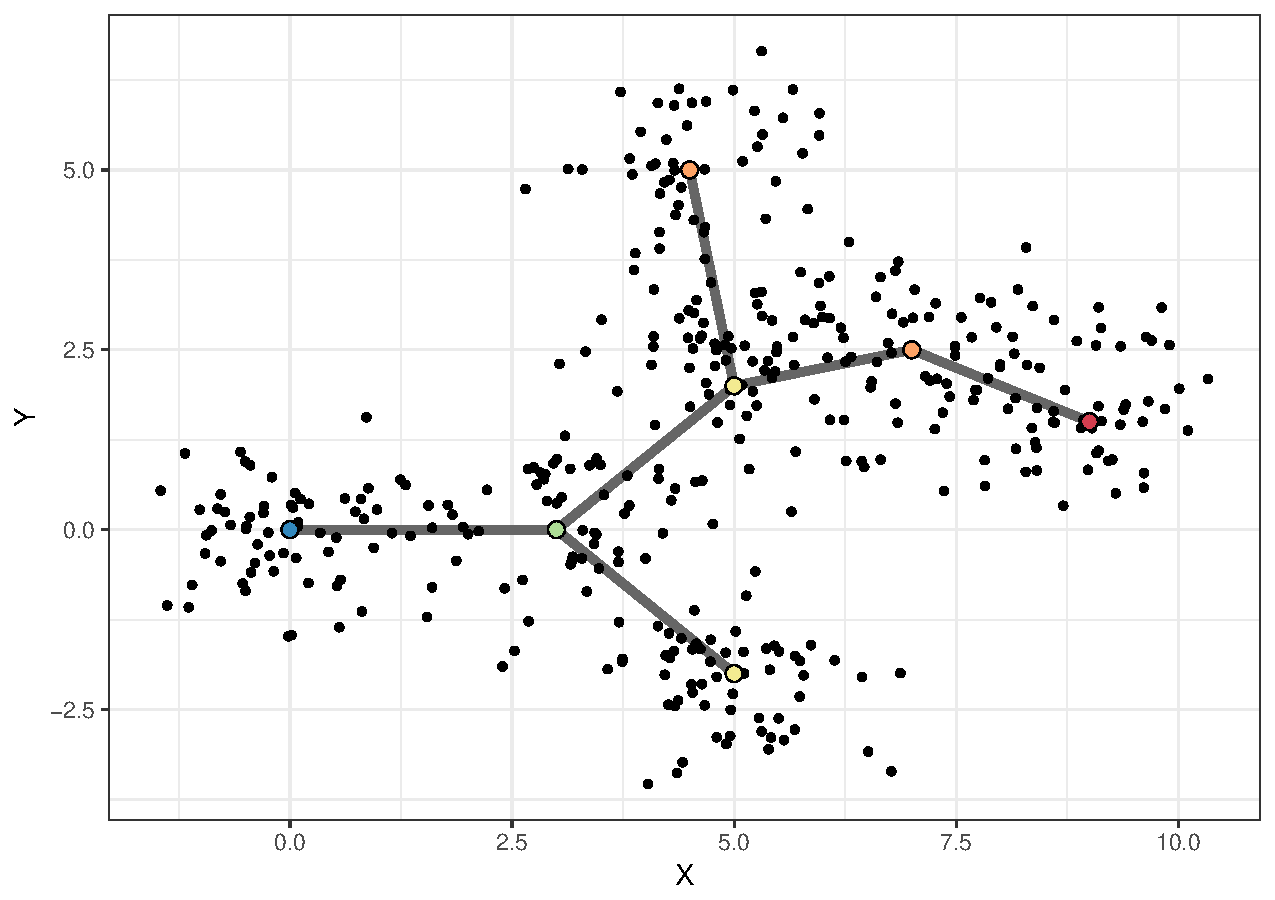
\includegraphics[width=.33\linewidth]{Img/Simulated/true}
    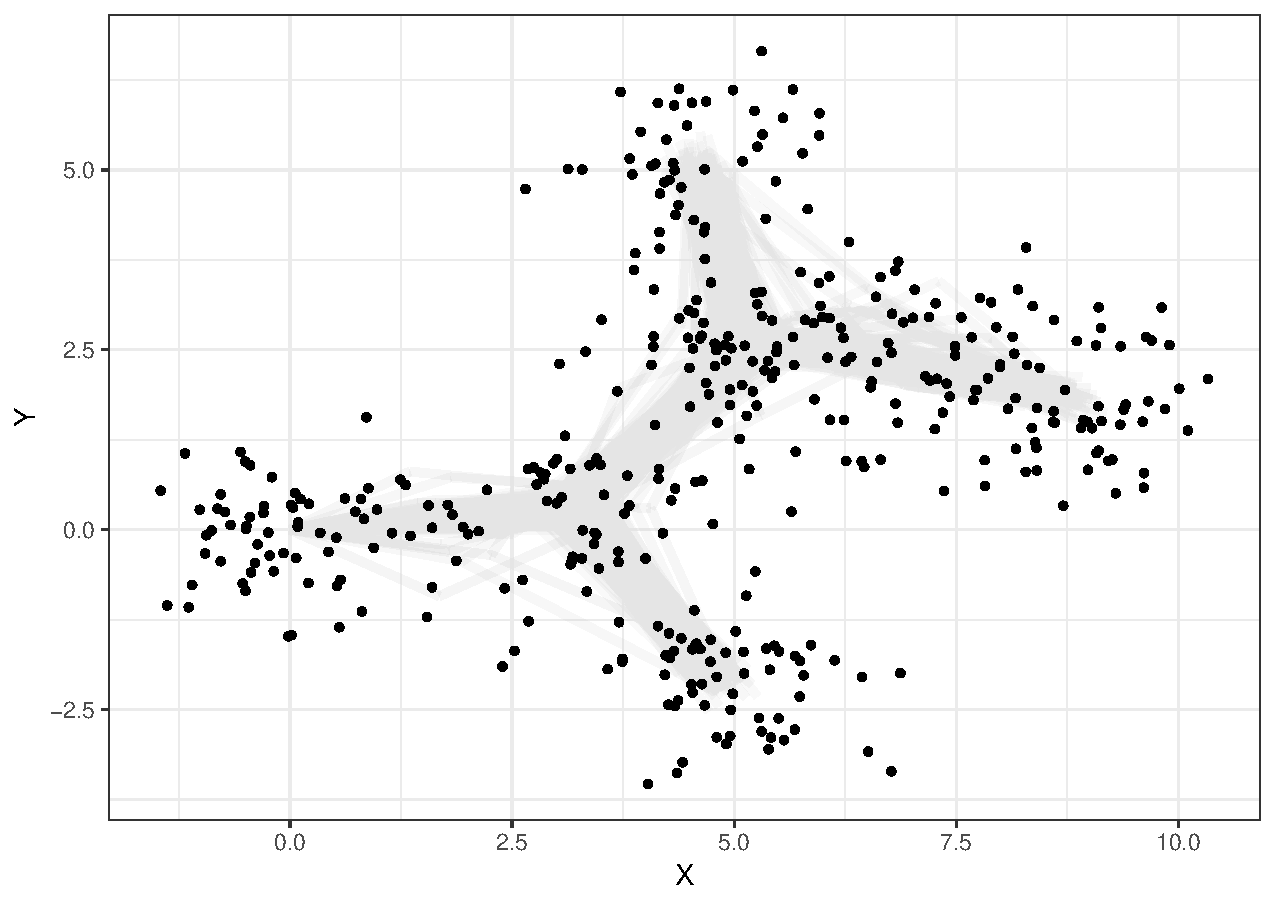
\includegraphics[width=.33\linewidth]{Img/Simulated/posterior_trees}
\caption{Fit of the s-MST model. The left panel shows the simulation
  truth. The right panel shows $M=500$ posterior samples of $\tau_k$.}
\label{fig:sim1_tree}
\end{figure}


\begin{figure}[!ht]
  \centering
    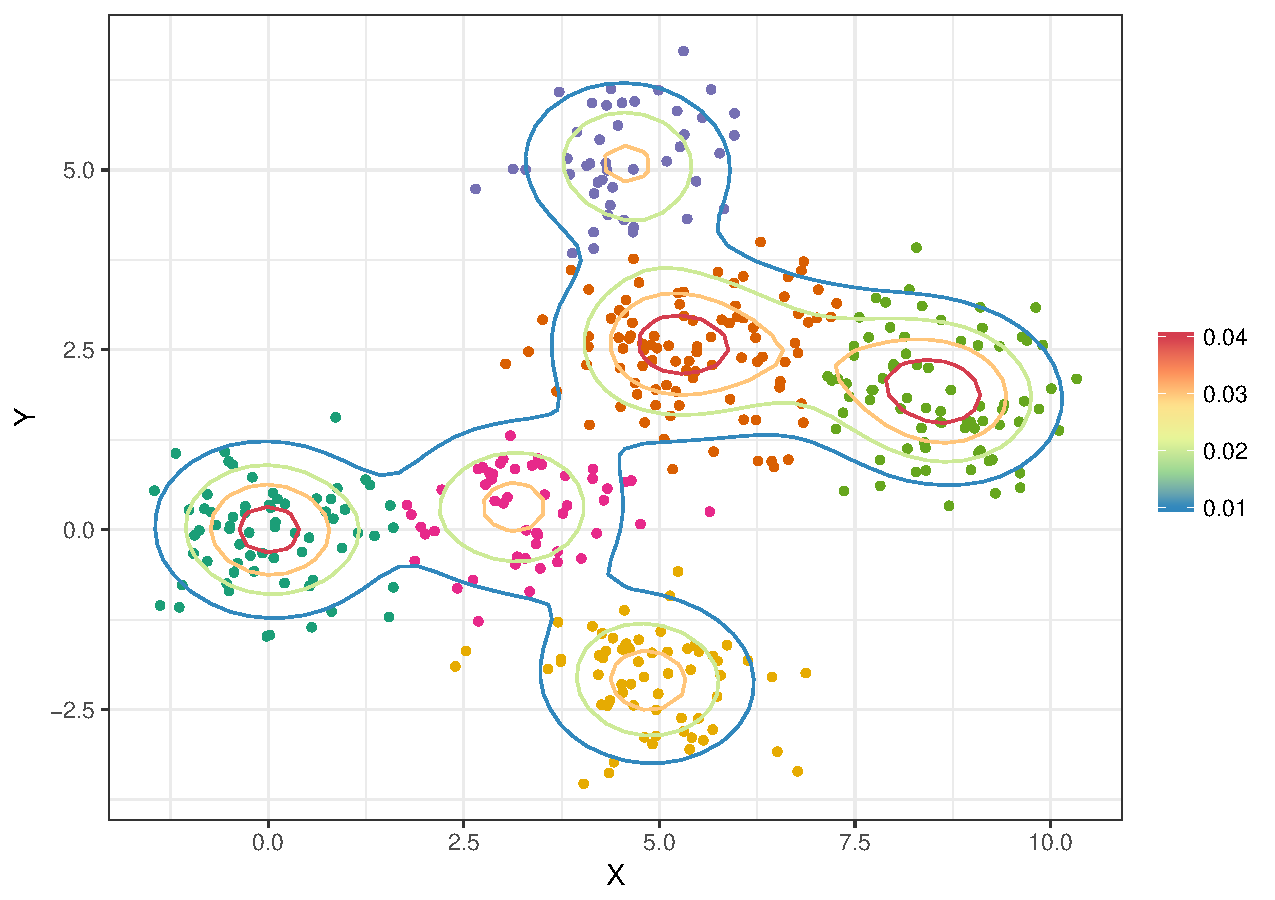
\includegraphics[scale = 0.4]{Img/Simulated/posterior_estimate}
\caption{Posterior density
  estimate obtained via the s-MST model. The observations are colored
  according to the optimal cluster labeling.}
\label{fig:sim1_dens}
\end{figure}


\subsubsection*{Hard MST}

Inference under the h-MST model is done via transdimensional MCMC according to Section \ref{sec:mst_inference} (full conditional distributions are described in Appendix \ref{sec:app_hmst}). First, we run very short parallel MCMC chains (5 iterations) with fixed number of components $k$ ranging from 2 to 15. In this first step, the full conditionals in Appendix \ref{sec:app_hmst} are computed using only the training data and transdimensional moves are not proposed. The second step consists of 10000 iterations of the transdimensional MCMC in which changes in the number of components $k$ are proposed as in Section \ref{sec:mst_inference} followed by the regular Gibbs sampling updates listed in Appendix \ref{sec:app_hmst}. Finally, cluster membership point estimates $\hat{\bfc}:=(\hat{c}_1, \ldots, \hat{c}_n)$ are obtained based on those 10000 iterations following \cite{wade2018bayesian}. Fixing $\bfc = \hat{\bfc}$  (which also implies a fixed posterior estimate on $k$) we run the update steps 2-5 in \ref{sec:app_hmst} for more 5000 iterations. 

Table \ref{tab:k_hmst_sim1} shows the results of the estimation of $k$ under different initial number of mixture components $k_0\in \{2,8,15\}$ and different fractions of training data $\epsilon \in\{0.1, 0.25, 0.5, 0.75\}$ reserved for proposing transdimentional moves. In general, the h-MST favors more parsimonious trees in comparison with the s-MST prior. Here, the results from both soft and hard models are quite similar. The h-MST model recovers 6 clusters for most configurations of $k_0$ and $\epsilon$. Notice how in the simulation, one of the centroids could be "erased" without causing big differences in the underlying tree. The h-MST therefore provided a more parsimonious tree in comparison with the s-MST.

Figure \ref{fig:sim1_multiple_trees_hmst} shows the posterior estimates on the MST structure and cluster membership for $k_0=8$ and $\epsilon=0.5$. The branching structure is well recovered by the h-MST model with six clusters instead of the simulated truth of 7, which was also observed with the s-MST. We can see that using one node less than the in the simulation true, did not compromise the overall branching structure of the tree.

% Table created by stargazer v.5.2.2 by Marek Hlavac, Harvard University. E-mail: hlavac at fas.harvard.edu
% Date and time: Wed, Mar 20, 2019 - 05:17:47 PM
%\begin{table}[!htbp] \centering 
%  \caption{Estimated number of clusters $k$ under the hMST model. The methodology of \cite{wade2018bayesian} was applied to the first 10000 iterations of the transdimensional MCMC under different choices of $\epsilon$ (fraction of data reserved as training) and $k_0$ (value of $k$ used in the initialization of the MCMC algorithm).} 
%  \label{tab:k_hmst_sim1} 
%\begin{tabular}{@{\extracolsep{5pt}} cccc} 
%\\[-1.8ex]\hline 
%\hline \\[-1.8ex] 
% & $k_0=2$ & $k_0=8$ & $k_0=15$ \\ 
%\hline \\[-1.8ex] 
%$\epsilon=0.1$ & $3$ & $6$ & $6$ \\ 
%$\epsilon=0.25$ & $4$ & $6$ & $6$ \\ 
%$\epsilon=0.5$ & $6$ & $6$ & $6$ \\ 
%$\epsilon=0.75$ & $6$ & $6$ & $6$ \\ 
%\hline \\[-1.8ex] 
%\end{tabular} 
%\end{table} 

\begin{table}[!htbp] \centering 
  \caption{Estimated number of clusters $k$ under the hMST model. The methodology of \cite{wade2018bayesian} was applied to the first 10000 iterations of the transdimensional MCMC under different choices of $\epsilon$ (fraction of data reserved as training) and $k_0$ (value of $k$ used in the initialization of the MCMC algorithm).} 
  \label{tab:k_hmst_sim1} 
\begin{tabular}{@{\extracolsep{5pt}} cccc} 
\\[-1.8ex]\hline 
\hline \\[-1.8ex] 
 & $k_0=2$ & $k_0=8$ & $k_0=15$ \\ 
\hline \\[-1.8ex] 
$\epsilon=0.1$ & $3$ & $6$ & $6$ \\ 
$\epsilon=0.25$ & $4$ & $6$ & $6$ \\ 
$\epsilon=0.5$ & $6$ & $6$ & $6$ \\ 
$\epsilon=0.75$ & $6$ & $6$ & $6$ \\ 
\hline \\[-1.8ex] 
\end{tabular} 
\end{table} 



%\begin{figure}[!ht]
%  \centering
%  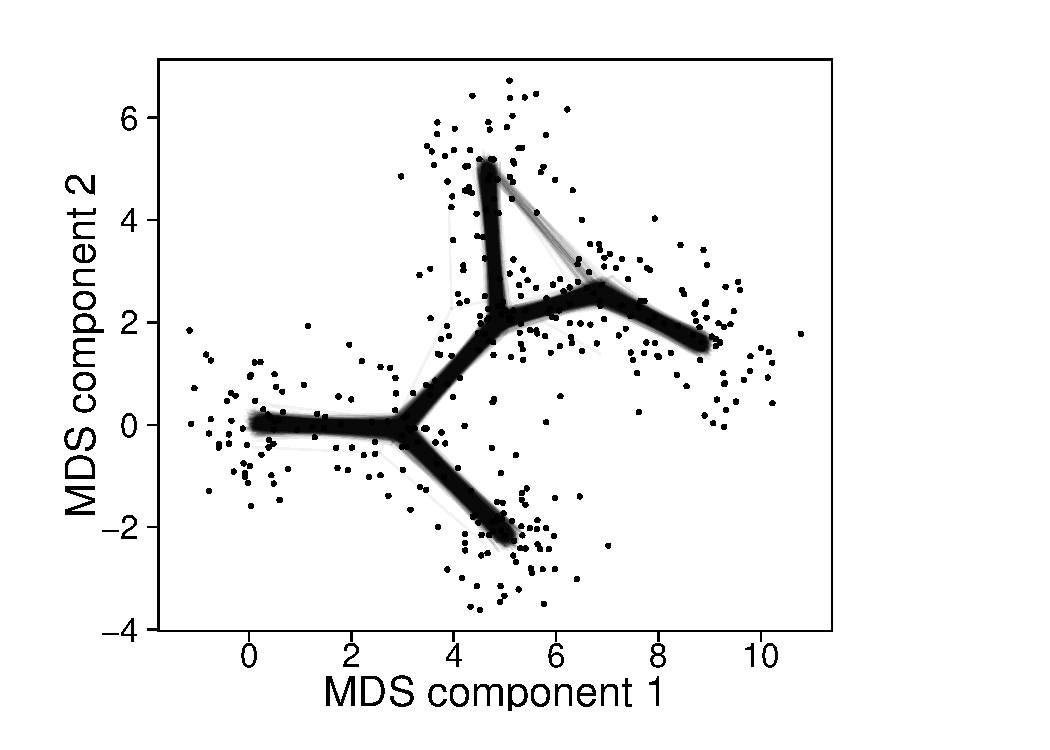
\includegraphics[width=.4\linewidth]{Img/Simulated/multiple_trees_sim1.pdf}
%    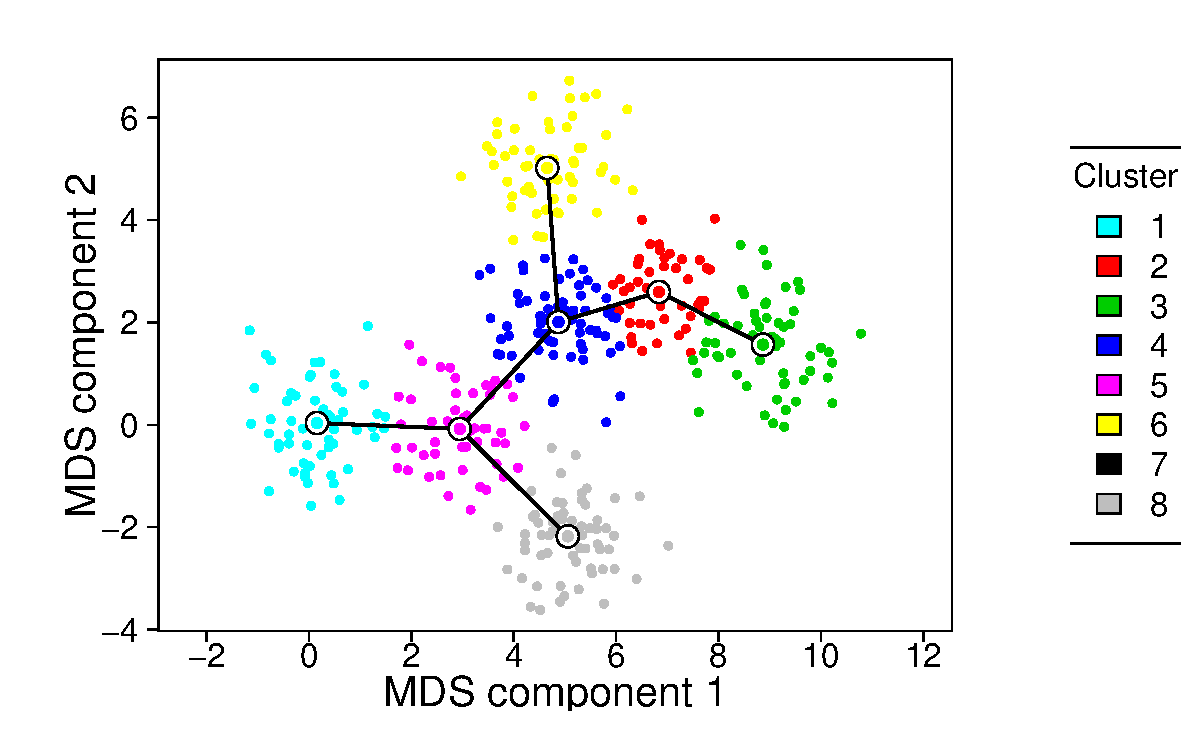
\includegraphics[width=.45\linewidth]{Img/Simulated/sim1_hmst_estimated_tree}
%\caption{Estimated branching structure of the hMST model with $k_0=8$ and $%\epsilon=0.5$ based on the last 5000 MCMC iterations (i.e., cluster membership indicators fixed at posterior estimate). Left panel: stochastic tree estimates under the hMST model. Right panel: multiple runs of slingshot applied to the simulated data.}
%\label{fig:sim1_multiple_trees_hmst}
%\end{figure}


\begin{figure}[!ht]
  \centering
  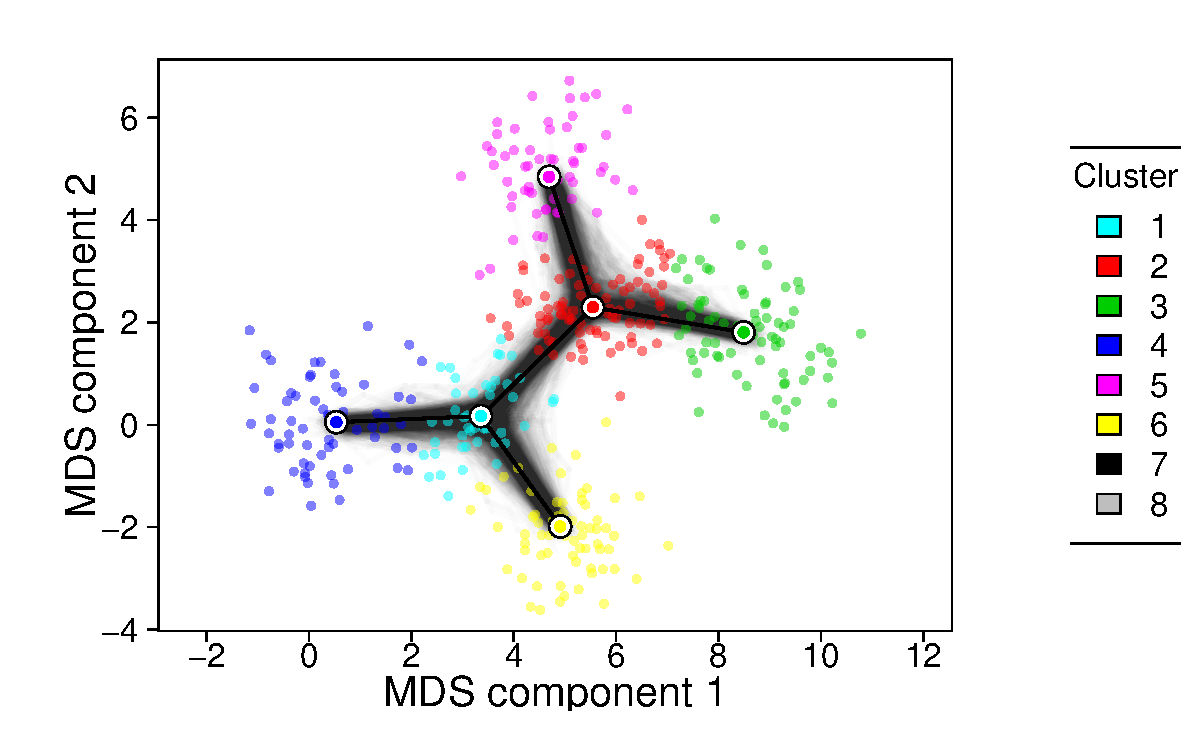
\includegraphics[scale = 0.5]{Img/Simulated/tree_all_in_one.pdf}
\caption{Estimated branching structure of the hMST model with $k_0=8$ and $\epsilon=0.5$ based on the last 5000 MCMC iterations. When the cluster membership indicators are fixed at the point estimate a posteriori, clusters 7 and 8 are empty.}
\label{fig:sim1_multiple_trees_hmst}
\end{figure}



\subsubsection*{Slingshot}

When analyzing the results of applying k-means (k=7) for recovering the clustering of cells followed by the slingshot algorithm to the simulated data, we noticed that some initializations lead to cluster structures that do not correspond to the truth under simulation. This issue is fixed once we consider a higher number of random initializations and select the one with best value of the objective function (Figure \ref{fig:sim1_slingshot_multipleK}). The slingshot algorithm is robust to the choice of $k$, specially when picking large values of $k$ in the k-means algorithm. The method however does not account for statistical uncertanty, which is accomodated in the s-MST and h-MST.

\begin{figure}[H]
  \centering
  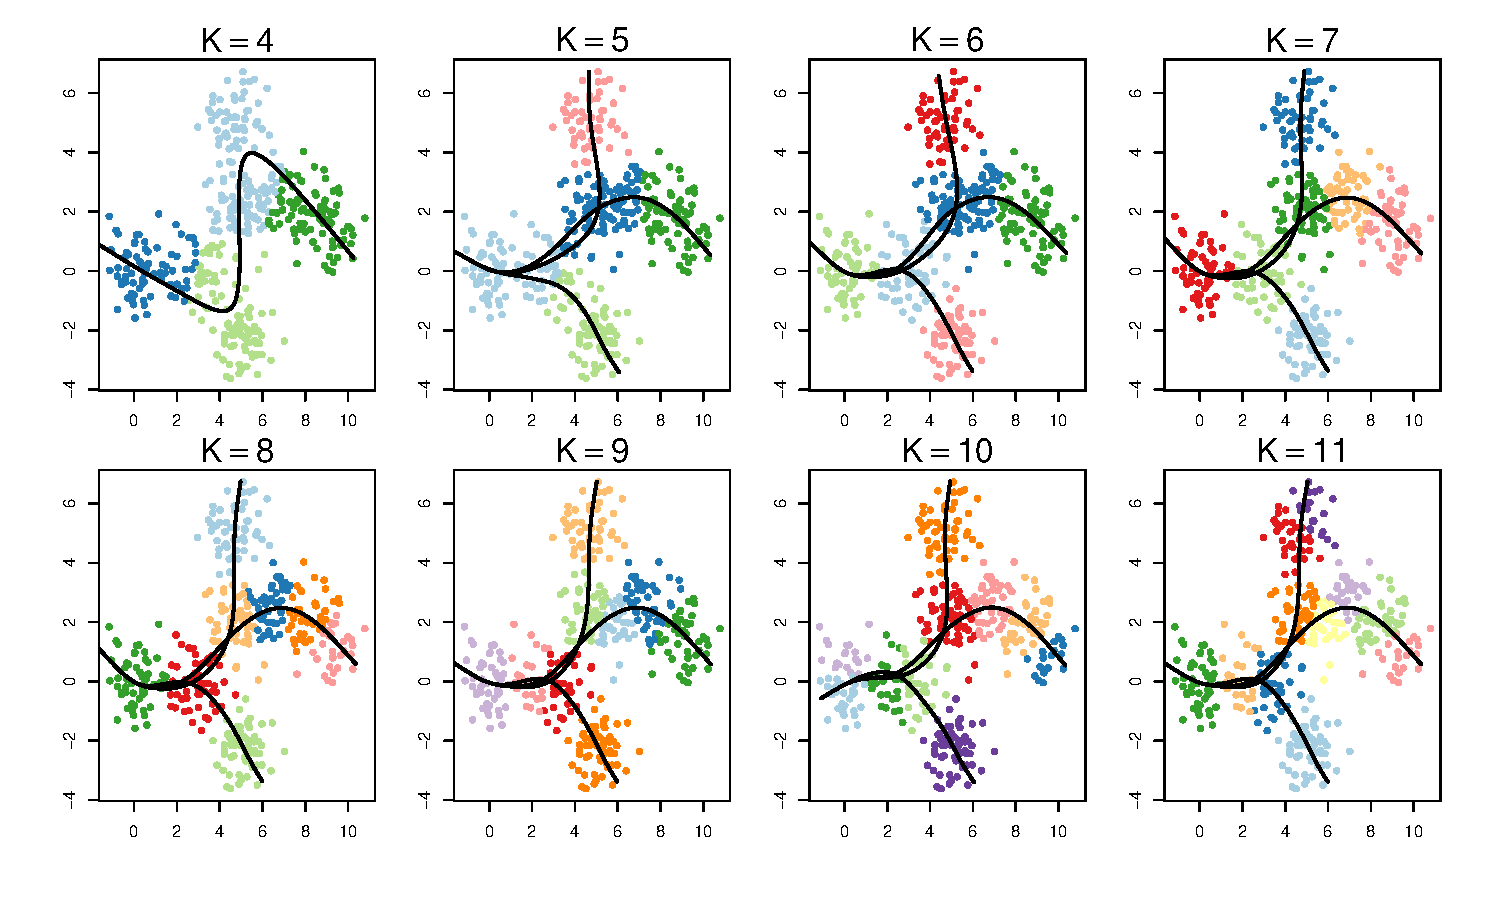
\includegraphics[scale = 0.5]{Img/Simulated/slinghot_sim_1_multipleK_2.pdf}
\caption{Parallel runs of slingshot applied to the simulated data for $k$ ranging from 4 to 11. Clusters are estimated by the best result among 10 random initializations of the k-means algorithm.}
\label{fig:sim1_slingshot_multipleK}
\end{figure}


\subsection{Simulation 2}

We now apply the algorithm to the same simulated dataset presented in
\cite{street2018}.  In Figure \ref{fig:sim2_groups} (left) we show samples from
the posterior on the trees. The density estimate in Figure
\ref{fig:sim2_groups} (right) fits the data well.


\begin{figure}[!ht]
  \centering
  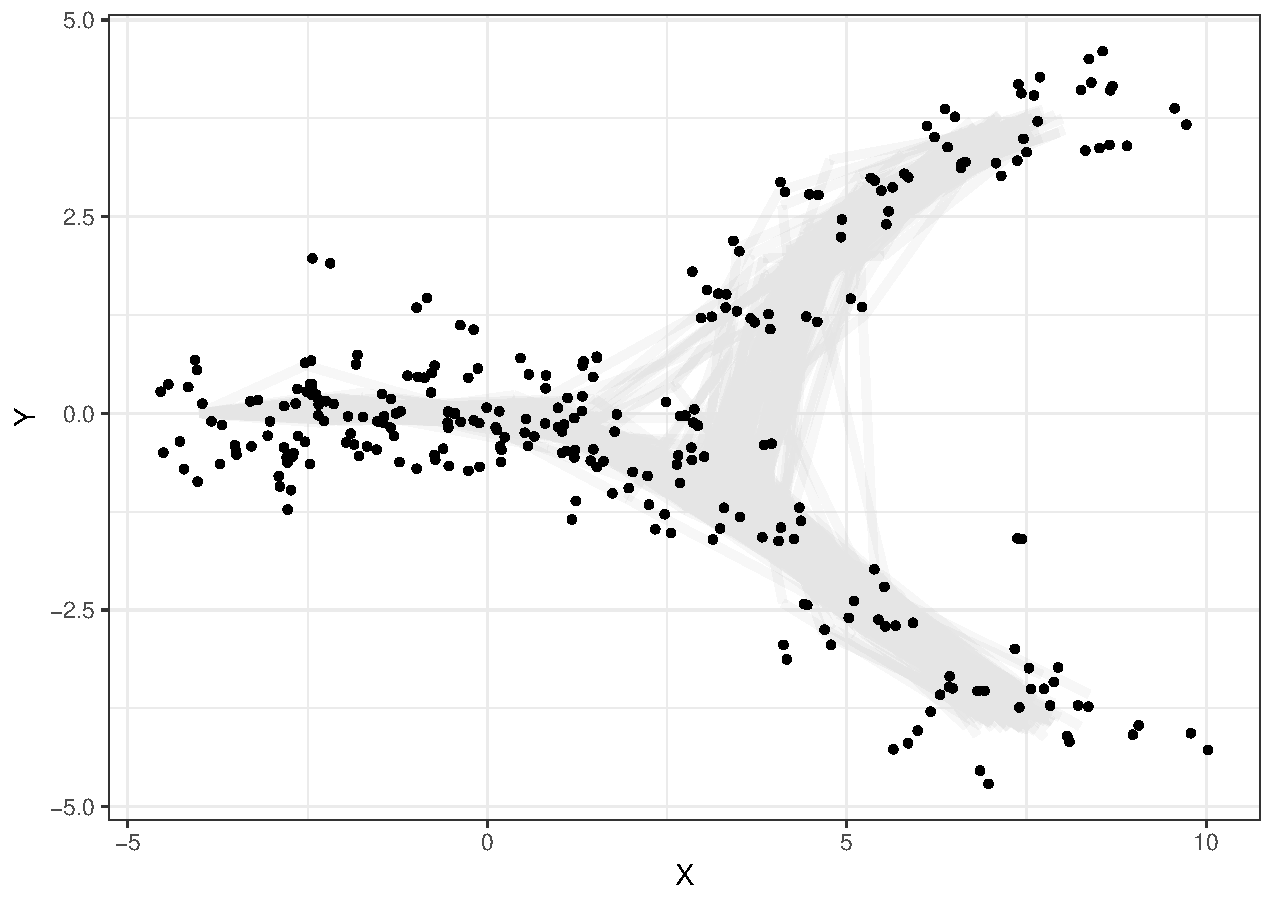
\includegraphics[width=.49\linewidth]{Img/Sim_slingshot/posterior_trees}
  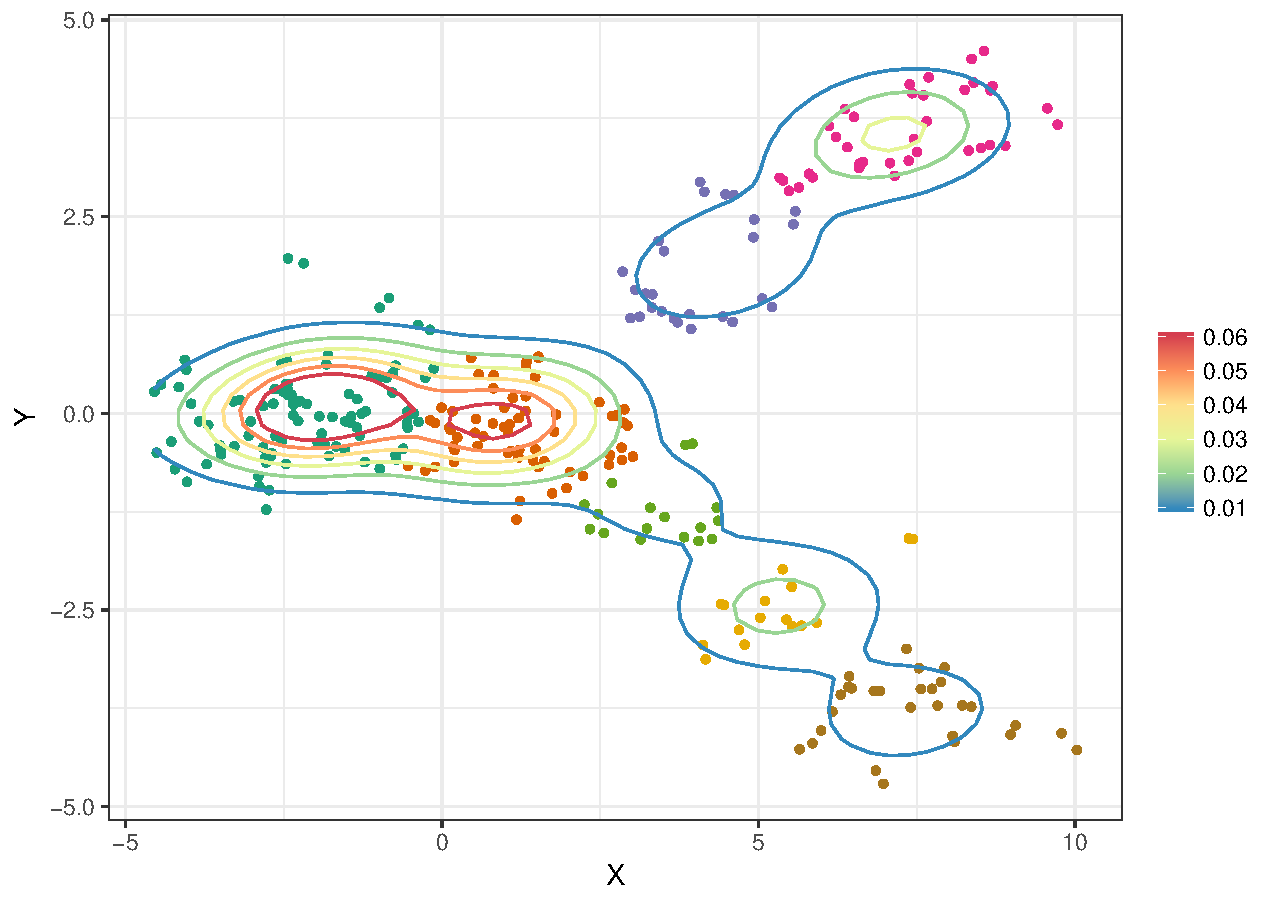
\includegraphics[width=.49\linewidth]{Img/Sim_slingshot/posterior_estimate}
\caption{Left panel: Plot of the posterior sampled trees. Right panel: posterior density estimate obtained via the s-MST model. The observations are colored according to the optimal cluster labeling.}
\label{fig:sim2_groups}
\end{figure}

\subsubsection*{Hard MST}
 
Again, we run 15000 iterations of MCMC on h-MST model. The first 10000 iterations include transdimensional proposal based on splitting the data into training and test, while the last 5000 are evaluated conditionally on the VI point estimate for the cluster membership structure. The h-MST model enforces more parsimony than the s-MST, which can be seen in Figure \ref{fig:sim2_hmst} as fewer components (five) are identified by MCMC.

%\begin{figure}[!ht]
%  \centering
%    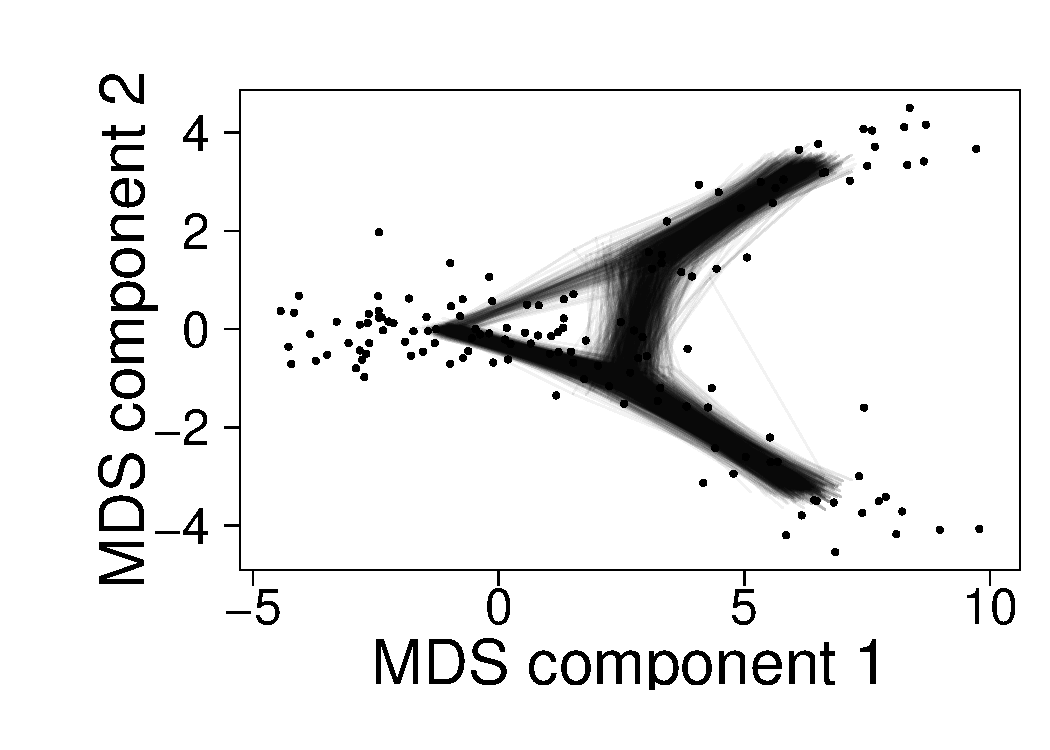
\includegraphics[width=.49\linewidth]{Img/Sim_slingshot/multiple_trees_slingshot_Kinit12.pdf}
%  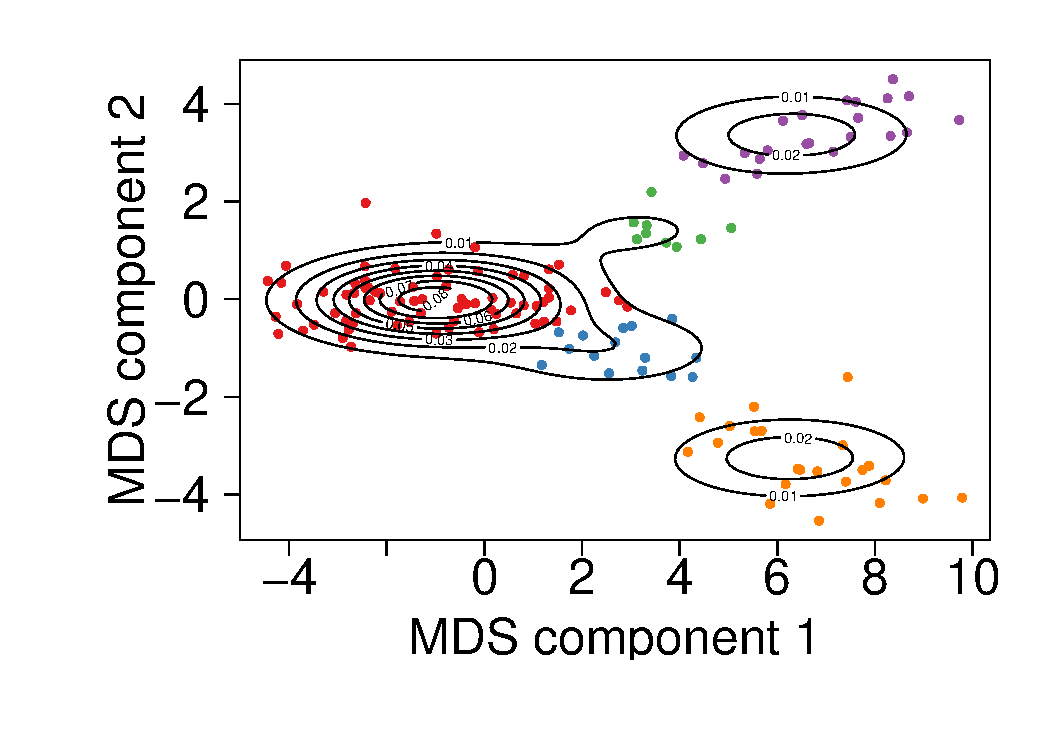
\includegraphics[width=.49\linewidth]{Img/Sim_slingshot/posterior_density_Kinit_12.pdf}
%\caption{Left panel: Sampled MST given the cluster membership estimates. Right panel: posterior density estimate obtained via the h-MST model. The observations are colored according to the optimal cluster labeling.}
%\label{fig:sim2_hmst}
%\end{figure}

\begin{figure}[!ht]
  \centering
  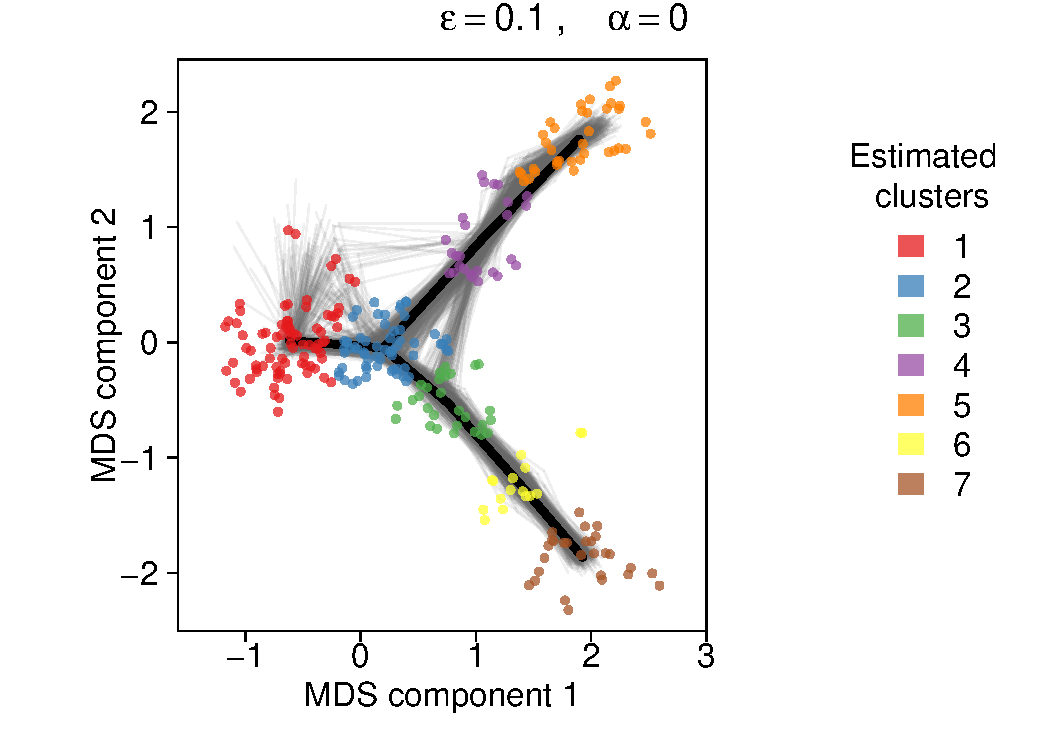
\includegraphics[width=.48\linewidth]{Img/Sim_slingshot/estimated_trees_slingshot_eps_01_xi_0.pdf}
  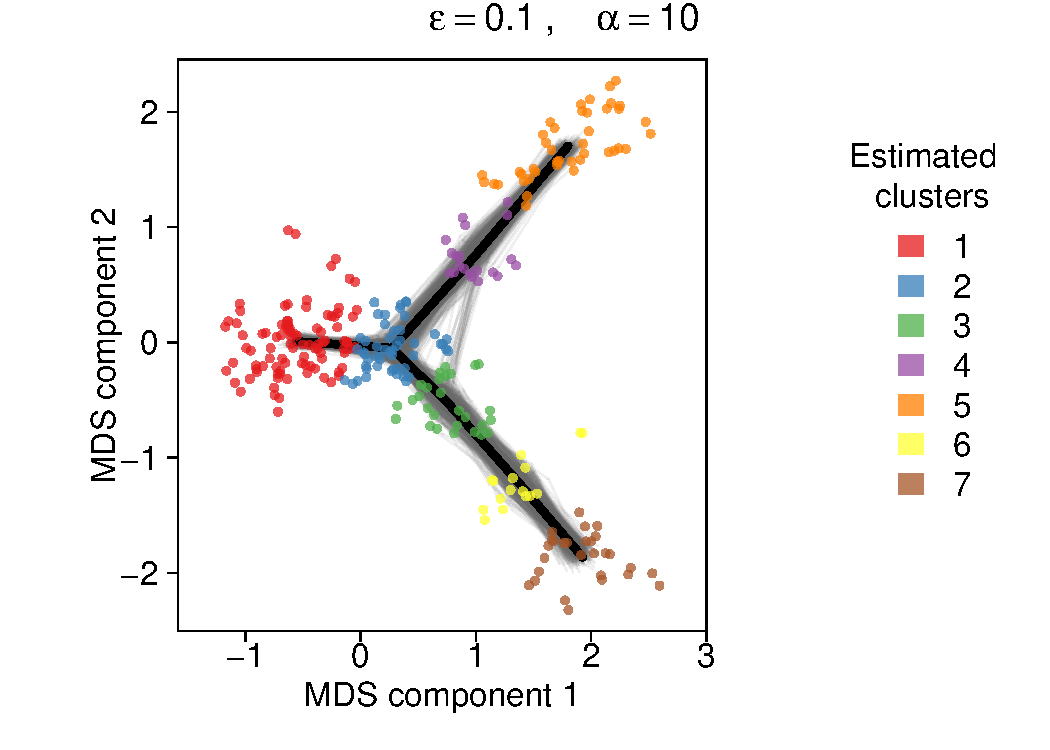
\includegraphics[width=.48\linewidth]{Img/Sim_slingshot/estimated_trees_slingshot_eps_01_xi_10.pdf}
\caption{Results of posterior estimation of MST. Curves in gray are the posterior sampled MST and the black tree in the point estimate a posteriori. $\alpha$ represents the strength of regularization towards simple MST structures that is implied by the hMST prior on $\bfmu$. $\epsilon$ is the fraction of the data reserved as training for the purpose of building the transdimensional proposals.}
\label{fig:sim2_hmst}
\end{figure}



\section{Mouse Data}

We  analyze data from 
a single cell RNA-seq experiment on horizontal basal cells (HBC) from the adult mouse
olfactory epithelium \citep{street2018}.
The goal is to infer the continuous progression from stem cells into
terminal mature cells and to estimate the cell-specific pseudotimes.

Due to the heterogeneity of cell populations, the analysis of
traditional transcription data, such as bulk microarrays, does not
allow researchers to discover cell dynamics. In fact, the underlying
signal can be potentially masked when averaging over thousands of
samples \citep{korthauer2016statistical},  possibly compromising
statistical power. 

The original data (before preprocessing) is available on GEO in
GSE95601 and also in
https://github.com/drisso/fletcher2017data. Preprocessing follows the steps in \citep{perraudeau2017}, which are listed here for completeness. The dataset originally contains measurements for 28284 genes throughout 849 cells. A total of 102 low-quality cells are removed from the dataset and the 1000 most variable genes are retained.

The resulting data is then normalized and the dimension is further
reduced to 50 by fitting a Zero-Inflated Negative Binomial-based Wanted Variation Extraction (ZINB-WaVE) model following \cite{zinbwave}. The ZINB-WaVE assumes a zero inflated negative bionomial model to extract low-dimensional signal from the data, accounting for dropouts (inflation of zeros), over-dispersion, and the count nature of the single cell RNA-seq data. Finally, multidimension scale (MDS) \citep{mardia1979} is applied to reduce the dimension further to 2 (this is the only deviation from \citealt{perraudeau2017} in which the dimension is reduced to 5). MDS consists of a rearrangement of the observations in a lower dimensional space (dimension 2 here) based on the matrix of pairwise distances computed using all the original 50 dimensions.

\paragraph*{Hard-MST model.}
We start by showing results of application of the model that enforces
MST structure (Section \ref{sec:model2_mst}). The RJMCMC was run for
3000 iterations. The first 2000 are used to obtain a point
estimate for the cluster membership indicators $c_i$ according with
\cite{dahl2006} and also for the number of mixture components
$k$. The final 1000 iterations are run with fixed $c_i$ and $k$.
The hyperparameters were chosen as $r_0 = 0.5$, $a_0=b_0=10$,
$\sigma^2_0=1$, $\lambda_0=1$ and $\delta=1$ to reflect
non-informative prior knowledge.


Figure \ref{fig:fletcher_est_tree} shows the estimation of the underlying minimum spanning tree. We estimate 8 nodes with one branching leaving the main path of the spanning tree (green). The right pannel illustrates the posterior uncertainty on the edges of the tree and highlights the proximity of green cluster with both the purple and the yellow clusters.


\begin{figure}[!ht]
  \centering
  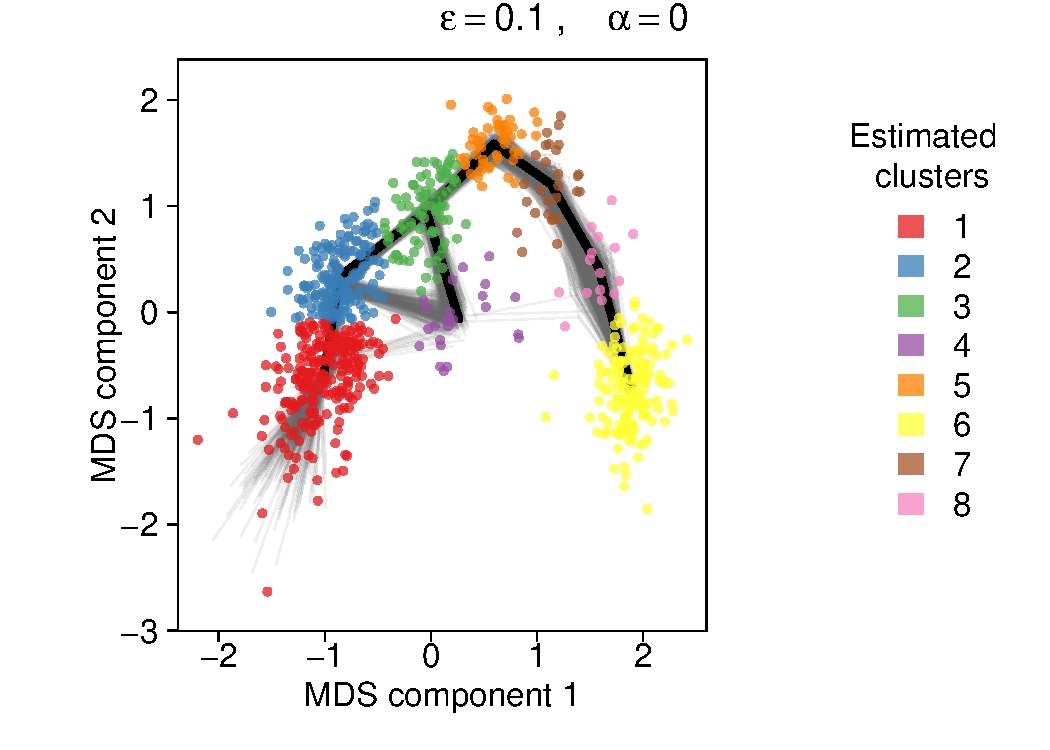
\includegraphics[width=.49\linewidth]{./Img/fletcher/estimated_trees_slingshot_eps_01_xi_0.pdf}
  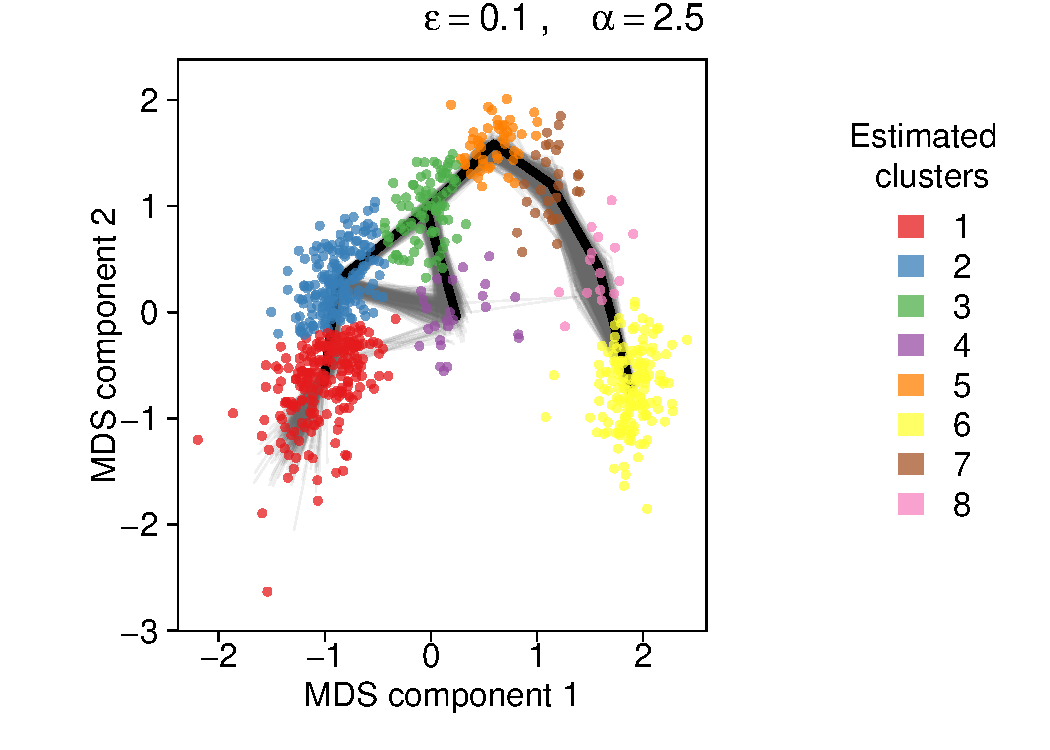
\includegraphics[width=.49\linewidth]{./Img/fletcher/estimated_trees_slingshot_eps_01_xi_25.pdf}
\caption{Posterior estimates of the latent MST and clustering membership structure based on the last 5000 MCMC iterations. Left panel: independent mixture ($\alpha = 0$). Right panel: MST dependent mixture ($\alpha=2.5$).}
\label{fig:fletcher_est_tree}
\end{figure}



We now focus on posterior estimation of pseudotimes. For each MCMC
sample (after burn-in) we construct a posterior sample for the
cell-specific pseudotimes as a deterministic transformation 
of the underlying MST. Such transformation is defined by calculating the
distance along the tree from its root node to the projection of the
cell onto the closest edge in the tree. 
 Let $T_i(\tau)$ denote the pseudotime for cell $i$. 
Figure \ref{fig:fletcher_est_pseudo}a
illustrates the evaluation of $T_i(\tau)$, 
where the
particular tree in the plot is fixed as the MST $\tau$ determined by the
posterior point estimates for the cluster centers. 
The right panel shows marginal posterior standard deviations for the
cell-specific pseudotimes,  conditional on cluster membership. 
Such graphical summaries help to identify those cells
that are more prone to missclassification for being at approximately
equal distance from two or more branches in the MST. 

%Figure \ref{fig:fletcher_hist}  shows the histogram of pseudotimes for cell
%707 (the one marked in black in Figure \ref{fig:fletcher_est_pseudo})
%in comparison with a typical cell from the green cluster (e.g, 730)
%and also from the black cluster (e.g., 631, 632). The small local mode
%near 0.1 indicates the proximity of cell 707 from those in cluster 2
%(black) and explains the high variance of its pseudotime a posteriori. 

\begin{figure}[!ht]
  \centering
  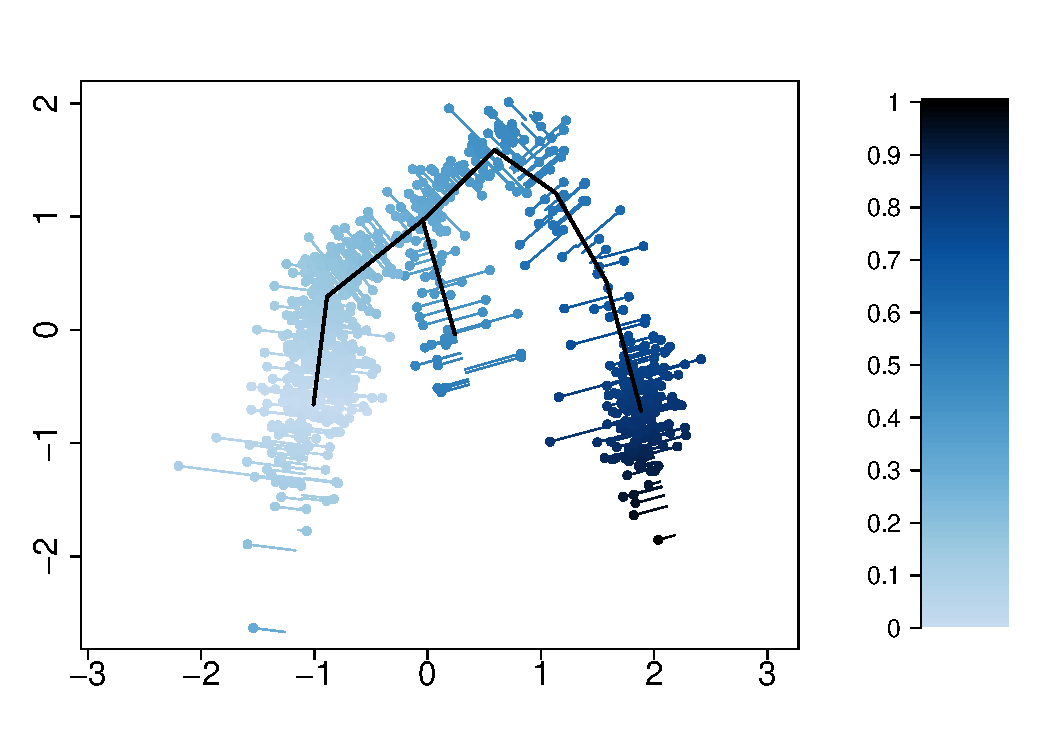
\includegraphics[width=.49\linewidth]{Img/fletcher/estimated_pseudotime_new.pdf}
  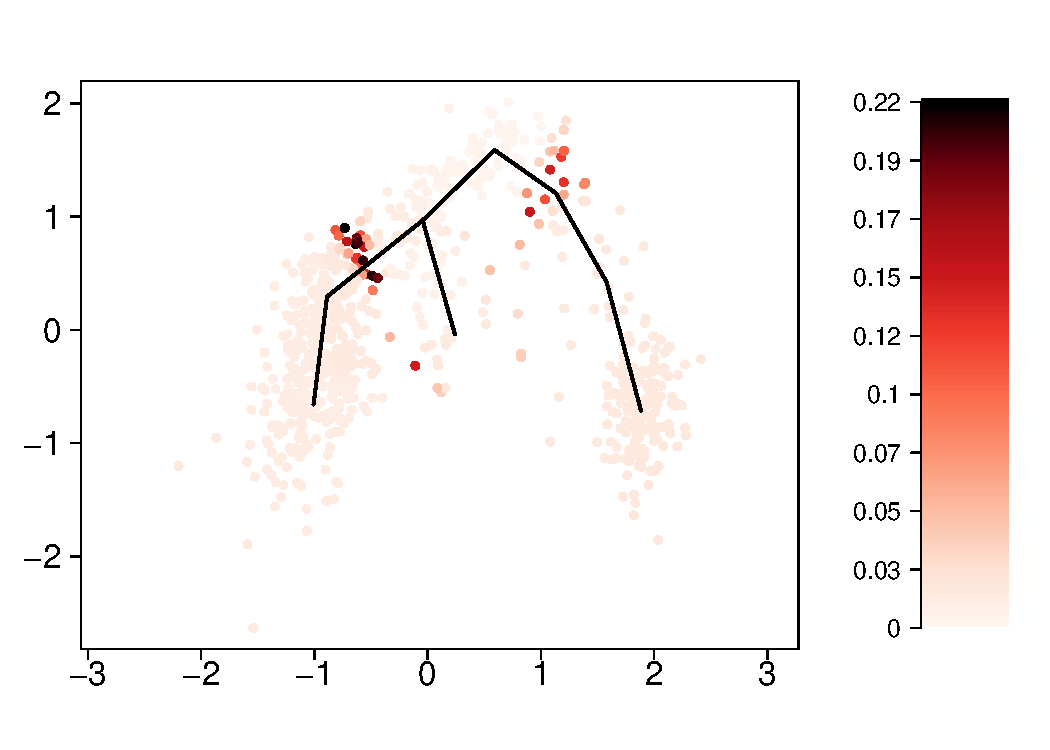
\includegraphics[width=.49\linewidth]{Img/fletcher/sd_pseudotime_new.pdf}
\caption{Left panel: Estimated pseudotimes for each cell. The extremes
  0 and 1 were chosen arbitrarily. 
  Right panel: posterior standard deviation of pseudotimes for each cell. Axis represent the two components of the MDS transformation.}
\label{fig:fletcher_est_pseudo}
\end{figure}


%\begin{figure}[!ht]
%  \centering
%  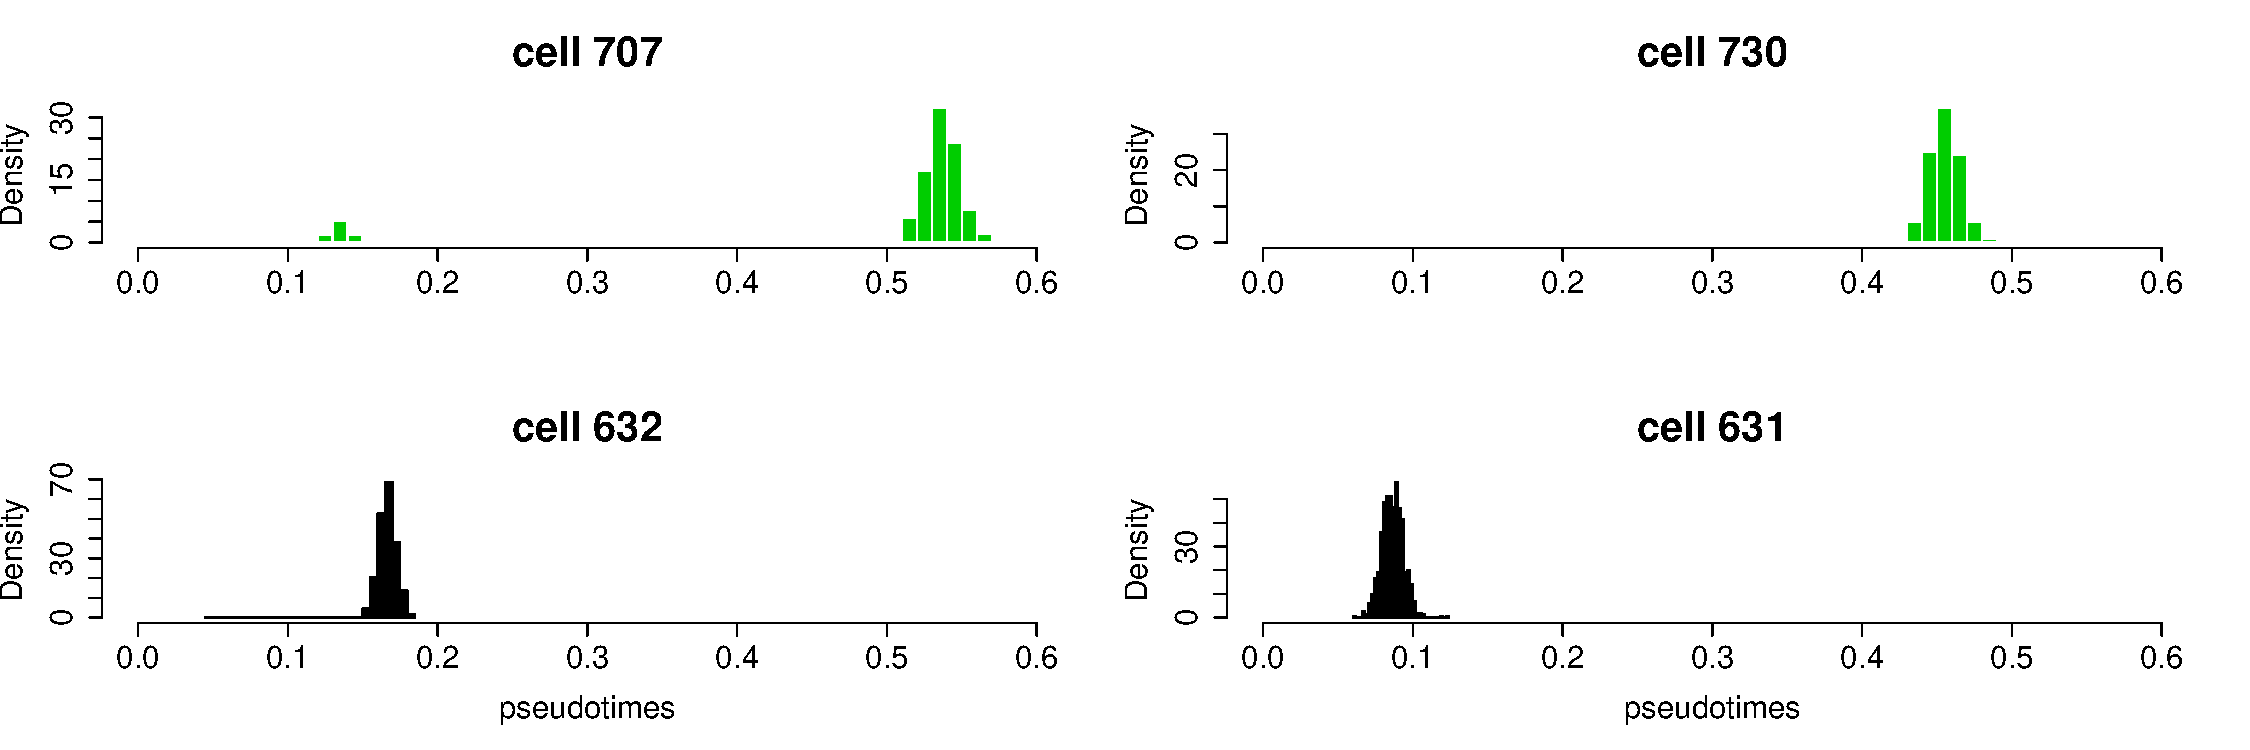
\includegraphics[scale = 0.4]{Img/fletcher/histograms.pdf}
%\caption{Posterior pseudotime distributions for two cells in clusters 2 and 5. }
%\label{fig:fletcher_hist}
%\end{figure}


In Figure \ref{fig:fletcher_boxplot}, we can have a broader view of
the estimated pseudotimes for cells in each one of the $k$ clusters. 

\begin{figure}[!ht]
  \centering
  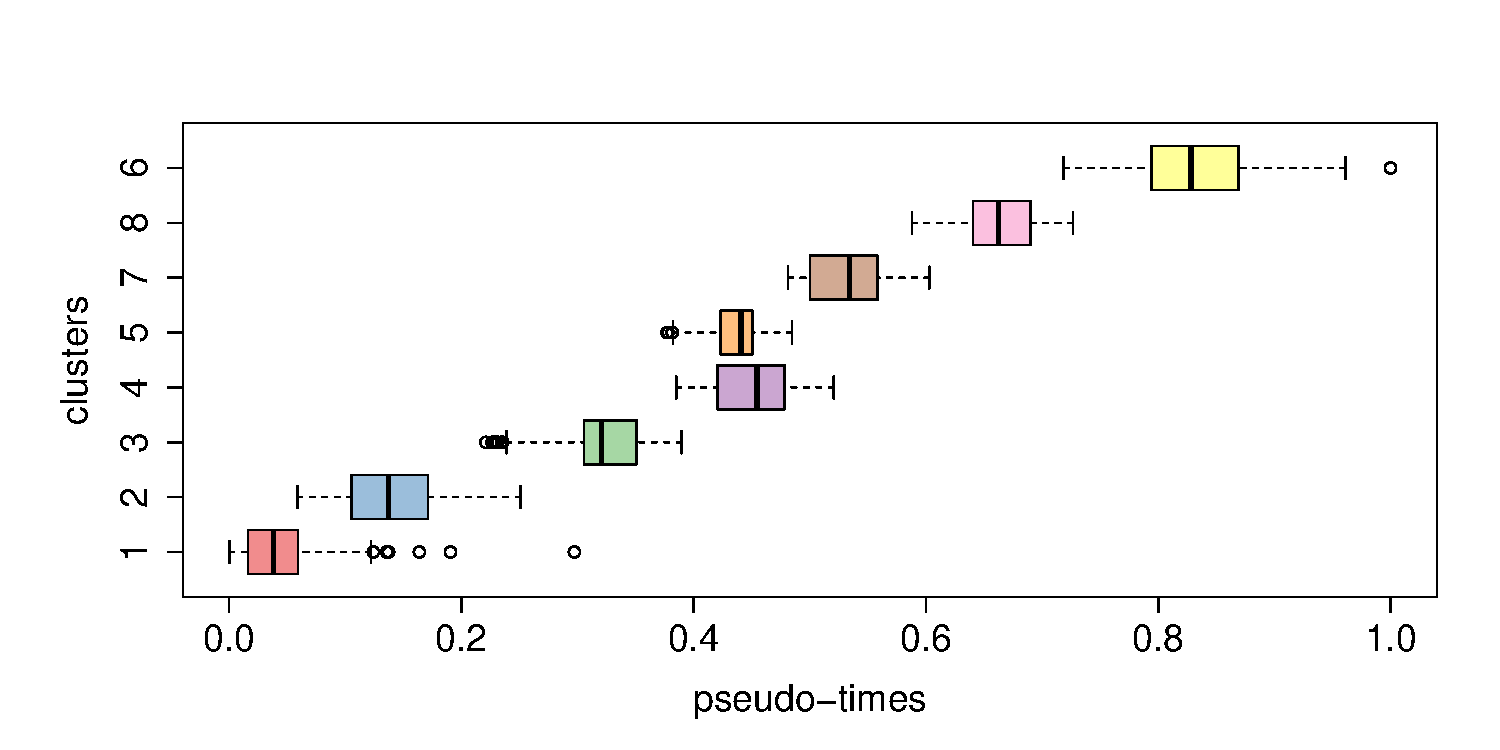
\includegraphics[scale = 0.4]{Img/fletcher/bp_pseudotime_new.pdf}
\caption{Cluster specific boxplots of median posterior pseudotimes obtained for each cell.}
\label{fig:fletcher_boxplot}
\end{figure}

\paragraph*{Slingshot.} The slingshot method is a multistep algorithm that produces an underlying MST conditional on a fixed estimate of the cluster centroids. The algorithm first computes the MST with the clusters' centroids as nodes. Then it fits for each leaf a principal curve that smooths the path from the root to that leaf along the corresponding branches of the MST. Each principal curve represents a cell different development path.

We now investigate the sensitivity of the slingshot method to the clustering of cells. We apply multiple independent runs of k-means algorithm initialized at random with k=8. Figure \ref{fig:fletcher_slingshot_kmeans} shows that the resulting MST is highly dependent on the initialization of the k-means algorithm, in some cases omitting important branches or creating artificial branches that clearly do not correspond to distinct cell populations. However, picking the best among multiple consistently solves the issue, as illustrated in Figure \ref{fig:fletcher_slingshot_kmeans2}.

\begin{figure}[H]
  \centering
  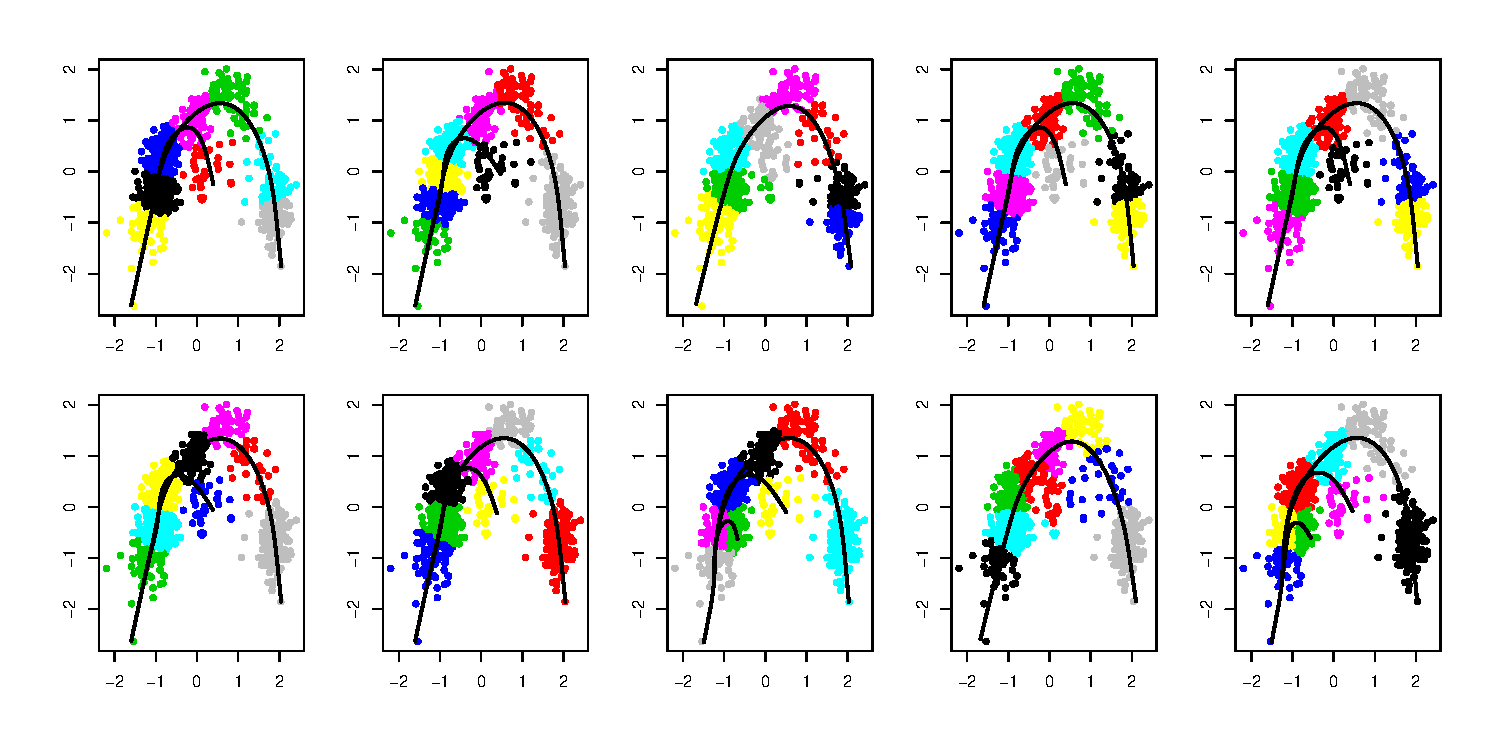
\includegraphics[scale = 0.55]{Img/fletcher/slinghot_estimates.pdf}
\caption{Multiple runs of slingshot applied to the mouse data. Each plot corresponds to a distinct random initialization of k-means algorithm (k=8). Axis represent the 2 MDS components for dimension reduction.}
\label{fig:fletcher_slingshot_kmeans}
\end{figure}

\begin{figure}[H]
  \centering
  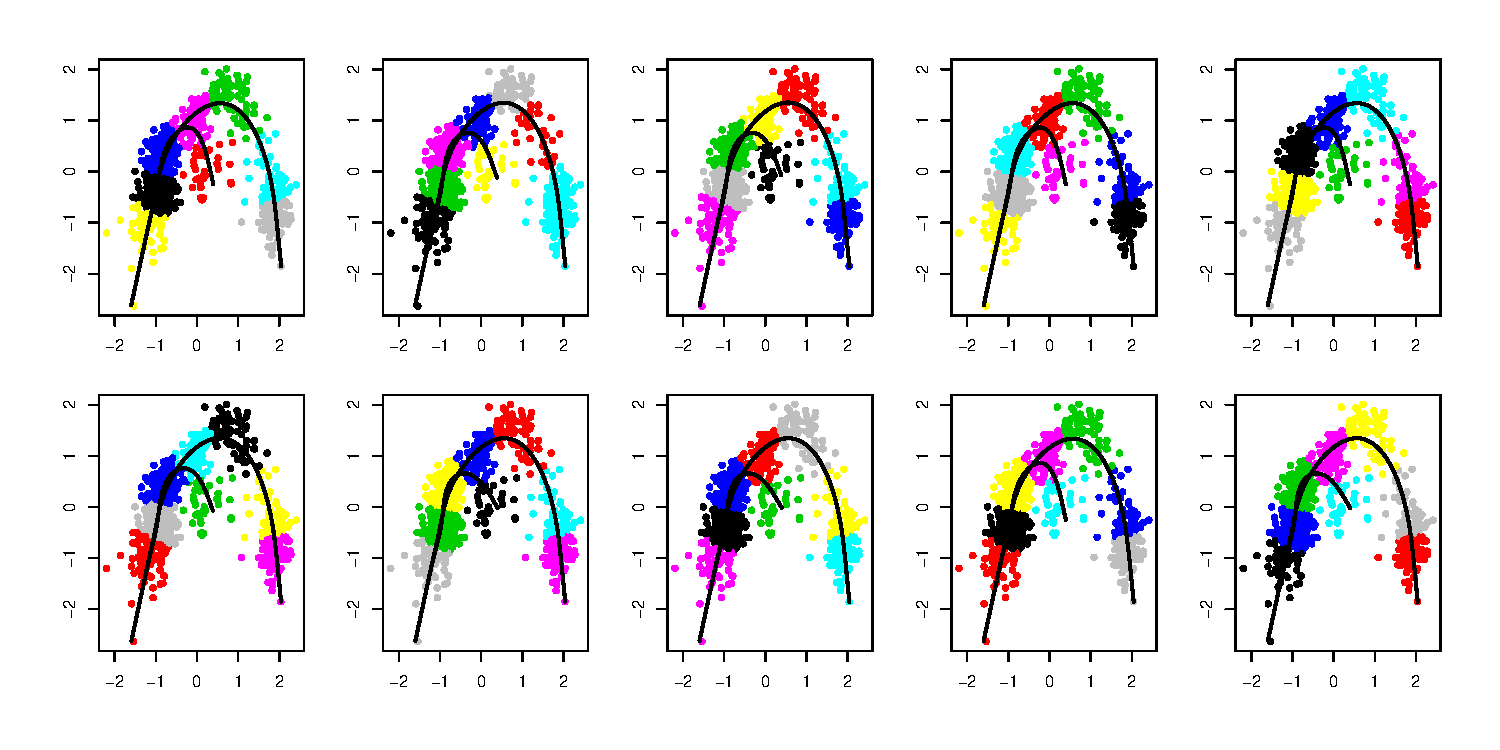
\includegraphics[scale = 0.55]{Img/fletcher/slinghot_estimates_rep.pdf}
\caption{Multiple runs of slingshot applied to the mouse data. Each plot corresponds to the best result among 10 distinct random initializations of k-means algorithm (k=8). Axis represent the 2 MDS components for dimension reduction.}
\label{fig:fletcher_slingshot_kmeans2}
\end{figure}

\section{Discussion}

We developed a dependent mixture model for single cell RNA sequencing data to estimate cell lineages. The proposed model takes into account the underlying tree in the transformed data on a lower dimension when defining the cluster structure of the cells: the model penalizes cluster allocations that define over complex trees. We presented two forms of defining such penalization terms: under soft MST or hard MST.

Motivated by the cell lineage applicaion, we deffined a dependent prior based on tree alignment. Other applications might give rise to dependence based on alignment of clusters on other, more general graphs.





 

\chapter{A Two Step Bayesian Model for Matching Cell Line and Patient Genomic Profiles}
\label{ch:cell_line_patients}
\index{Instructions for Preparing Dissertations, Theses, and Reports%
@\emph{Instructions for Preparing Dissertations, Theses, and Reports}}%

\section{Introduction}
\label{sec:intro}

In a precision medicine paradigm, the patient's specific genetic architecture is assessed to propose a personalized treatment that is expected to be optimal for that individual. In this context, there is a trend in modern medicine to move from generalized treatment approaches towards the tailored treatment strategy that is dictated by their genomics or molecular profile. This paradigm shift accelerates the needs for advances in pharmacogenomics technology and associated analytical methods. In this paper, we develop methods to meet this demand, inclduing in particular novel priors for random structures. Briefly, we propose  developing an integrative statistical framework, that merge  multiplatform genomics ('omics, in short) profiles from multiple model systems (e.g. patients and cell-lines) for finding significant drug targets, pre-clinical models for appropriate drug discovery and repurposing  and, finally, to calibrate therapeutic potential for future patients. By identifying these similarities (and differences) across model systems, we are able to gather more refined information about the patient than what is contained in their specific profile, while still proposing a personalized treatment that is strongly tied to the patient's profile - through appropriate integration of various data sources. 

The objective of this paper is then to construct a novel Bayesian statistical  approach for  matching patient gene profiles with cell line profiles. Such inference is needed, among many other applications, for data integration, precision medicine and patient specific treatment assignment. The expansion of modern medicine and fast growth of research in health sciences  have  led to a great increase in available  data on multiple sources/platforms such as The Cancer Genome Atlas (TCGA, \url{tcga-data.nci.nih.gov}), Cancer Cell Line Encyclopedia (CCLE, \url{portals.broadinstitute.org/ccle}), International Cancer Genome Consortium (ICGC, \url{icgc.org}) to name a few.  A model-based approach  for matching of a patient profile with data from other sources, such as from cell lines, allows us to access a  wider range of information to predict a patient’s response to specific treatments. Important for the envisioned application, the matching should be carried out on the basis of a biologically meaningful signal only, putting aside mere noise.

A cell line is a culture of cells extracted from a tissue (e.g.,
cancer cells from a tumor in a human tissue) and grown in an in-vitro
environment that simulates the environment of the tissue in the
organism where it was extracted. Therefore, cell lines serve as
models to study cancer biology.  Information  from the response to a
drug or treatment applied to cell lines (cultivated {\it in-vitro}) is used
to infer about the  expected response {\it in vivo}
\citep{goodspeed2016}. Similarly, individuals can be grouped
according to similarities between their profiles and observed profiles
in a fixed set of cell lines.
 In such scenarios,  the mapping of
cell lines and patients  opens the possibility to construct treatment
recommendations 
based on results for the corresponding cell lines \citep{sinha2015}. We propose a statistical  approach that seamlessly  combines the
output of the Bayesian mixture model
 based on a proposal by \cite{poe_2002} with a novel two-way Bayesian non-parametric (BNP) mixture model  that is constructed as an extension of a  BNP bi-clustering model of \cite{lee2013}. 

\cite{poe_2002} propose a Gaussian-uniform mixture model for probability of expression
 (POE). Later in the model construction we shall use the latent trinary signal of the POE model to carry out nested clustering of patient samples and the desired matching with cell lines. The uniform component in the POE models havier tails associated with genes that are over- and under-expressed, while the Gaussian term corresponds to regularly expressed genes. The authors argue that, by trichotomizing  gene expressions into these 3 categorical levels, the POE approach smoothly removes uninformative biological and instrumental noise that is naturally present in genomic profile data, therefore strengthening downstream  analysis.

The clustering of patient samples and the desired match with cell lines builds on a model developed of \cite{lee2013}, who present a Bayesian model  (NoB-LoC)  that identifies genes (columns) that are relevant for clustering of samples/individuals (rows).  The identified genes are then partitioned  in such a way that genes within the same subgroup (column-wise clusters)  give rise to a common nested partition of individuals (row-wise clusters). 
 The approach is motivated by the observation that high-dimensional protein profiles make it hard to find meaningful
clusters of samples/individuals. Researchers therefore often restrict attention to groups of proteins that are
expected to lead to more meaningful and interpretable results. NoB-LoC identies such groups in a seamless process, together with the nested clustering of samples. The NoB-LoC model conveniently allows for different clustering of samples with respect to different groups of proteins. In our context, this translates to association of cell lines and patients depending on the set of proteins in the profile.



Developing the outlined model consturction, this chapter makes two major contributions: the first one is the  integration of POE with the two-way clustering building on the NoB-LoC model. The second, and perhaps more important contribution is the extension of the NoB-LoC model to allow for explicit probabilistic matching of profiles that could come from distinct sources (e.g., cell
lines and patients). In short,  in the proposed approach we first use the NoB-LoC model to partition the proteins 
according to a zero enriched P\'olyia urn process where some proteins are set aside as inactive proteins, while the selected proteins are grouped into protein clusters (active proteins). Within each protein cluster, the samples are partitioned again, using a partition model that matches patients to cell lines. The motivation is that the usually high-dimension protein profiles make it hard to find similar samples to be clustered together, therefore restricting the attention to groups of proteins is expected to lead to more meaningful and interpretable results. This procedure also naturally allows for identification of co-expressed proteins in the form of protein clusters, i.e. a group of genes that are biologically correlated are also expected to have their expression levels "tied together" along different samples. Finally, the NoB-LoC model conveniently allows for different clustering of samples depending on the subsample of proteins that is considered. In our problem, this translates to association of cell lines and patients depending on the set of proteins in the profile.

The real data used in the statistical analysis comes from an experiment using reverse phase protein arrays (RPPA)
which record the expression of selected proteins simultaneously on multiple cell lines and patients samples \citep{rppa_ref}. The dataset analyzed here consists of lung cancer protein expressions (233 proteins) measured in 687 patients and 124 cell lines. Data is batch corrected, i.e., they are also adjusted for the batch effect difference between cell line and patients' data).

\section{ POE Model}
\label{sec:poe}

In this section we describe the POE (probability of expression) model defined in \cite{poe_2002}. We modified some of the priors in order to obtain analytical full-conditionals for as many parameters as possible, which facilitates the MCMC implementation in the larger, encompassing model (more details ahead and also in appendix \ref{sec:full_cond}).

Each observation $y_{sg}$ consists of expression levels for protein (gene) $g\in \{1, \dots, G\}$ and sample $s \in \{1, \dots, S\}$. Latent variables $e_{sg}$ indicate high expression of gene $g$ in sample $t$ ($e_{sg} = 1$), normal expression ($e_{sg} = 0$) and under expression ($e_{sg} = -1$). Each possible value of $e_{sg}$ determines a different distribution for the observed gene expressions according to the following Gaussian-Uniform mixture model

$$(y_{sg} \mid e_{sg}) \sim \begin{cases}
Unif(\alpha_s + \mu_g, \ \alpha_s + \mu_g + k^+_g), &\mbox{ if } e_{sg} = 1,\\
N(\alpha_s + \mu_g, \ \sigma^2_g), &\mbox{ if } e_{sg} = 0,\\
Unif(\alpha_s + \mu_g - k^-_g, \ \alpha_s + \mu_g), &\mbox{ if } e_{sg} = -1.
\end{cases}$$\\

The lengths  $k^+_g$ and $k^-_g$ of the support of the uniform components should cover the tails of the corresponding gene expression distribution implying heavier tails than the Gaussian distribution. Under normality, the great majority of the samples (probability 0.997) concentrate within 3 standard deviations from the mean; therefore the constraints $k^+_g > k_0 \sigma_g, \ k^-_g > k_0 \sigma_g$ imply heavier than Gaussian tails for fixed values of $k_0$ greater than, say, 3. 

We now define the weights for each term in the mixture by the probability vectors $\bfpi_g:=(\pi^-_g, \pi^0_g, \pi^+_g), \ g \in \{1, \dots, G\}$ where $\pi^+_g = P(e_{sg} = 1 \mid \bfpi_g) $, $\pi^0_g = P(e_{sg} = 0 \mid \bfpi_g)$ and $\pi^-_g = P(e_{sg} = -1 \mid \bfpi_g).$ We assume $(\bfpi_g \mid \bfeta_{\pi}) \sim Dirichlet(\bfeta_{\pi}).$

Figure \ref{fig:poe_ex} illustrates the implied mixture model in the context of density estimation. The augmentation of the parameter space with inclusion of indicatior variables  $e_{st}$ allows for identification of up- and down-regulated genes that are not well captured bythe light tails of a single Gaussian component.

\begin{figure}[!ht]
  \centering
  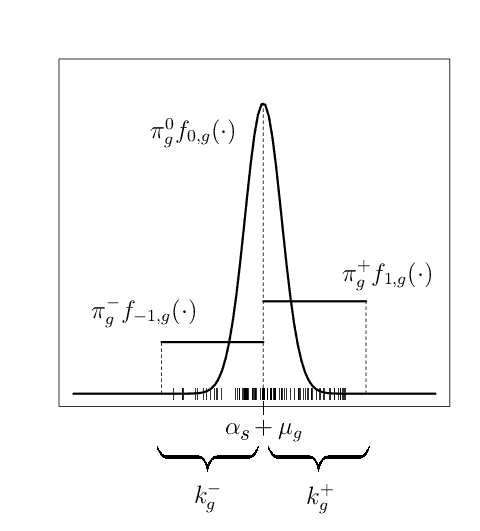
\includegraphics[scale = 0.5]{./veera/ex_poe_a_mod.png}
  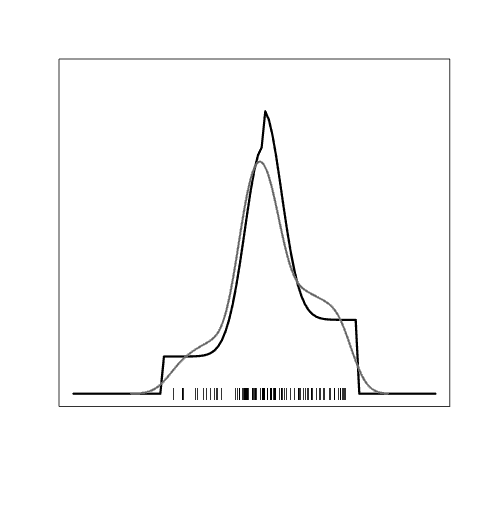
\includegraphics[scale = 0.5]{./veera/ex_poe_b.png}
\caption{Left panel: Weighted components of the Gaussian-Uniform mixture model. Right panel: density estimates using Gaussian-Uniform mixture (black line) and using kernel estimate (gray line). Vertical bars represent data generated from the Gaussian-Uniform mixture.}
\label{fig:poe_ex}
\end{figure}


Posterior probabilities of differential expression are determined by Bayes rule as 
\begin{align}
p^+_{sg} &:= P(e_{sg} = 1 \mid y_{sg}, \bfpi_g, f_{1,g}, f_{0,g}) \nonumber \\
&=\frac{\pi^+_g f_{1,g}(y_{sg})}{ \pi^+_g f_{1,g}(y_{sg}) + \pi^0_g f_{0,g}(y_{sg}) + \pi^-_g f_{1,g}(y_{sg})}\times \mathds{1}(y_{sg} \in S_{f_{1,g}}) \nonumber \\
&=\frac{\pi^+_g f_{1,g}(y_{sg})}{ \pi^+_g f_{1,g}(y_{sg}) + \pi^0_g f_{0,g}(y_{sg})}\times \mathds{1}(y_{sg} \in S_{f_{1,g}}), 
\label{eq:p+}
\end{align}

\noindent where $\mathds{1}(\cdot)$ is the indicator function and $S_{f_{1,g}}$ denotes the support of $f_{1,g}$. Analogously,

\begin{align}
p^-_{sg} :&= P(e_{sg} = -1 \mid y_{sg}, \bfpi_g, f_{-1,g}, f_{0,g}) \nonumber\\
&=\frac{\pi^-_g f_{-1,g}(y_{sg})}{ \pi^-_g f_{-1,g}(y_{sg}) + \pi^0_g f_{0,g}(y_{sg})}\times \mathds{1}(y_{sg} \in S_{f_{-1,g}}).
\label{eq:p-}
\end{align}

Equations \eqref{eq:p+} and \eqref{eq:p-} are used for visualization of sample specific gene profiles. Since $p^+_{sg}$ and $p^-_{sg}$ are not simultaneously positive, the differences $d_{sg}:=p^+_{sg} - p^-_{sg}$ will fall in the interval $[-1,1]$, therefore serving as a unidimensional measure of gene expression ( $d_{sg}\approx 1$ for highly expressed and $d_{sg}\approx -1$ for underexpressed genes).

The model is completed by the prior specification $(\mu_g \mid \theta_{\mu}, \tau_{\mu}) \sim N(\theta_{\mu}, \tau_{\mu}), $
$(\alpha_s \mid \mu_{\alpha}, \tau_{\alpha}) \sim N(\mu_{\alpha}, \tau_{\alpha}) \mbox{ restricted to } \sum^S_{s=1} \alpha_s = 0,$
$(\sigma^2_g \mid \gamma, \lambda) \sim InvGamma(\gamma, \lambda),$
$(k^+_g \mid \alpha_{k^+}, \beta_{k^+}) \sim InvGamma(\alpha_{k^+}, \beta_{k^+}),$
$(k^-_g \mid \alpha_{k^-}, \beta_{k^-}) \sim InvGamma(\alpha_{k^-}, \beta_{k^-}).$ We also chose prior models for hyperparameters as $\theta_{\mu} \sim N(m_{\mu}, s^2_{\mu})$,
$\tau_{\mu} \sim InvGamma(a_{\tau_{\mu}}, b_{\tau_{\mu}})$,
$\alpha_{k^+} \sim Exp(\lambda_{\alpha_{k^+}})$,
$\alpha_{k^-} \sim Exp(\lambda_{\alpha_{k^-}})$,
$\beta_{k^+} \sim Gamma(a_{\beta_{k^+}}, b_{\beta_{k^+}})$,
$\beta_{k^-} \sim Gamma(a_{\beta_{k^-}}, b_{\beta_{k^-}})$.
\end{enumerate}

 The motivation to propose Inverse Gamma priors for $k^+_g$, $k^-_g$ and Dirichlet prior for $\bfpi_g$ is to make use of conjugacy results in the full-conditional posterior of these parameters, which was not originally explored in \cite{poe_2002}. 

\subsection{Posterior inference for the POE model}

We implement posterior inference by MCMC simulation. All full conditionals are available in closed form due to the choice of contditionally conjugate priors/hyperpriors; the only exceptions are $\alpha_{k^+}$ and $\alpha_{k^-}$. We therefore implement Gibbs sampling transition probabilities for all parameters except $(\alpha_{k^+} \mid \bfy, else)$ and $(\alpha_{k^-} \mid \bfy, else)$. For the latter we use Metropolis-Hastings transition probabilities with random walk proposal on $\log \alpha_{k^+}$ and $\log \alpha_{k^+}$ respectively. See appendix \ref{sec:full_cond} for more details.

To avoid numerical instability when sampling from truncated inverse gamma distributions (full conditional posterior distributions for $k^+_g$ and $k^-_g$), we used a variable augmentation scheme proposed in \cite{damien2001}. The prior on the auxiliary variables introduced by the authors imply full-conditional posterior distributions for those variables, which are sampled together with the original parameters of the POE model within the full MCMC algorithm.

\section{Nonparametric Bayesian Clustering with Patient and Cell Line Matching}
\label{sec:nobloc2}

\subsection{ A nested random partition and matching structure}
\label{sec:nobloc_matching}

Following posterior simulation for the POE model, the posterior estimated values $d_{sg}$ become the inputs for model-based clustering of proteins and samples and the desired pairing with cell lines. This is implemented by the construction of a nested partition model that builds on the Nonparametric Bayesian local clustering (NoB-LoC) model defined in \cite{lee2013}. In this section, we relabel the data $d_{sg}$ as $d^c_{ig}$ if sample $s$ corresponds to the $i$-th cell line or as $d^p_{ig}$ if it is the $i$-th patient. The subindex $g$ still denotes protein $g$. We will assume the dataset contains $G$ proteins and $S$ samples, including $N^p$ patient samples and $N^c$ cell line samples ($N^p + N^c = S$).


The model first partitions the proteins according to a zero enriched P\'olya urn. One special cluster (corresponding to the zero-enrichment) is interpreted as "inactive proteins". The remaining ones are grouped into protein clusters (active proteins). Within each of these protein clusters, the samples are partitioned again by a second, nested partition model. The nested partition model includes also the desired pairing of each patient sample cluster with a matching cell line. 

Consider the cluster membership indicator $w_g$ for each protein $g=1, \ldots G$ and denote $\bfw=(w_1, \ldots, w_{G})$ the vector of protein cluster indicators. Let $\pi_0$ be the probability of inactivation and let $\alpha_0> 0$ be the potential for creating a new cluster. Finally, define $n_k:= \#\{g; \ w_g=k\}$ the number of proteins that fall into protein cluster $k$, for $k=0, 1, \ldots, K_{\bfw}$ with $k=0$ denoting the cluster of inactive proteins and $K_{\bfw}$ denoting the total number of active clusters of proteins determined by $\bfw$. Then the zero enriched P\'olyia urn defines $p(\bfw \mid \pi_0)$ as

\begin{equation}
p(\bfw \mid \pi_0) = \pi^{n_0}_0(1-\pi_0)^{G-n_0} \times \frac{\alpha^{K_{\bfw}}_0 \prod^{K_{\bfw}}_{k=1}\Gamma(n_k)}{ \prod^G_{g=1} (\alpha_0 + g - 1)},
\end{equation}

\noindent and for short we write $(\bfw \mid \alpha_0, \pi_0) \sim ZEPU(\alpha_0, \pi_0)$.

For each cluster of proteins defined by $\bfw$, two dependent partitions of the samples are defined, the first one involving patients only, and the second one (which is stochastically  dependent on the partition of patients) includes only cell lines. The cluster membership indicators for the $i$-th patient and  $i$-th cell line in $k$-th cluster of proteins are defined as $\delta^{p,k}_i$ and $\delta^{c,k}_i$, respectively. The two partitions are then determined by the cluster membership indicators for patients and for cell lines. We marginally model the cluster membership of patients $\bfdelta^{p,k}:= (\delta^{p,k}_i)^{N^p}_{i=1}$ as $\bfdelta^{p,k}\sim ZEPU(\alpha_{pk}, \pi_{pk})$. This implies a random number $J_k$ of active clusters of patients within the $k$-th group of proteins.

Conditionally on $\bfdelta^{p,k}$, several choices of priors on $\bfdelta^{c,k}$ are possible, each of them representing one way of matching cell lines' to patients' profiles.\\

\noindent \textbf{Discrete uniform prior:} we assume a discrete uniform prior for $\bfdelta^{c,k}$ on the patient samples and the set of inactive samples: $\delta^{c,k}_i \mid \bfdelta^{p,k} \sim Uniform( \{0, 1,\ldots, J_k\})$.\\

\noindent \textbf{Discrete uniform prior with at most $\ell$ cell lines per cluster of samples:} the conditional prior on $(\bfdelta^{c,k} \mid \bfdelta^{p,k})$ has the  p.m.f 
\begin{equation}
p(\bfdelta^{c,k} \mid \bfdelta^{p,k}) \propto \mathds{1}(\bfdelta^{c,k} \in \mathcal{B}^{c,k}_{\ell})
\label{eq:support_disc_unif}
\end{equation}

\noindent with support 

\hspace{-1 cm}$\mathcal{B}^{c,k}_{\ell}=\left\{(\delta^{c,k}_i)^{N^c}_{i=1} \in \{0, 1, \ldots, N^c\}^{N_c}; \ \ \ \sum^{N^c}_{i = 1} \mathds{1}(\delta^{c,k}_i = j)\leq \ell \ \forall j \in \{1, \ldots J_k\} \right\}.$

\noindent In the special case $\ell = 1$ for example, the multiplicative normalization constant in equation \eqref{eq:support_disc_unif} is $\sum^{ \min\{J_k, N^c\} }_{n=0} {J_k \choose n} {{N^c}\choose n} n!$ \ .

%\noindent \textbf{Centroid based categorical distribution:} a categorical distribution on $\{0, 1, \ldots, J_k\}$ is assumed for $\delta^{c,k}_i \mid \bfdelta^{p,k}$ in which $P(\delta^{c,k}_i = j \mid \bfdelta^{p,k}) \propto || \bar{\theta}_{j} - ||$

\noindent \textbf{Conditional zero inflated Polya urn:} a conditional zero inflated Polya urn prior distribution is assumed prior for $\bfdelta^{c,k} \mid \bfdelta^{p,k}$ as a continuation of the process of clustering patient samples. This means that the initial probability of allocation of cell lines to a patient cluster is proportional to the cluster size. Stochastically, this approach is equivalent to a joint zero inflated Polya urn for all samples.\\


We consider the Gaussian sampling model $(d^c_{ig}\mid\theta^c_{ig},\sigma^2_g) \sim N(\theta^c_{ig}, \sigma^2_g)$ and $(d^p_{jg}\mid\theta^p_{ig},\sigma^2_g)  \sim N(\theta^p_{jg}, \sigma^2_g)$ for cell line $i$ and patient $j$ and protein $g$. The prior for $\theta^x_{ig}$ with $x$ being either $c$ or $p$ is

\begin{align}
\theta^x_{ig}\sim
\begin{cases}
I_{\theta^*_{jg}}, \ &\mbox{ if  } \delta^{x, w_g}_i = j > 0 \mbox{ and } w_g > 0 \mbox{ (active prot. and smpl.)}\\
N(\mu_{1g}, \sigma^2_{1g}), &\mbox{ if  } \delta^{x,w_g}_i = 0 \mbox{ and }w_g>0 \mbox{ (active prot. inactive smpl.)} \\
N(\mu_{2g}, \sigma^2_{2g}), &\mbox{ if  } w_g=0 \mbox{ (inactive prot.)},
\end{cases}
\label{eq:unique_mean}
\end{align}

\noindent where $I_{x}$ denotes the point mass distribution (Dirac measure) at $x$. In \eqref{eq:unique_mean} (first equation) we define the unique mean responses $\theta^*_{jg}$ for active proteins and samples. We denote by $J_k$ the number of active sample clusters for all proteins $g$ such that $w_g=k$. Notice that active cell lines and patients share the same mean response if they belong to the same sample cluster. 

For the purpose of deriving the MCMC algorithm for posterior inference, we marginalize the patient specific (and cell line specific) means $\theta^x_{ig}$ in \eqref{eq:unique_mean}, which implies the following data distribution

\begin{equation}
d^x_{ig} \sim
\begin{cases}
N(\theta^*_{jg}, \sigma^2_g) \ &\mbox{ if  } \delta^{x, w_g}_i = j > 0 \mbox{ and } w_g > 0 \mbox{ (active prot. and smpl.)}\\
N(\mu_{1g}, \sigma^2_{1g} + \sigma^2_g), &\mbox{ if  } \delta^{x,w_g}_i = 0 \mbox{ and }w_g>0 \mbox{ (active prot. inactive smpl.)} \\
N(\mu_{2g}, \sigma^2_{2g} + \sigma^2_g), &\mbox{ if  } w_g=0 \mbox{ (inactive prot.)}.
\end{cases}
\label{eq:unique_mean_2}
\end{equation}

The prior for the unique mean response values is specified as $\theta^*_{jg} \sim N(\mu_{0g}, \sigma^2_{0g})$ with hyperpriors $\sigma^{-2}_{g} \sim Gamma(a_g, b_g)$, $\tau^{-2}_{lg} \sim Gamma(a_{lg}, b_{lg})$ and $\mu_{0g}, \ \mu_{1g}, \ \mu_{2g} \stackrel{iid}{\sim} N(m_0, s^2_0)$.

\subsection{Summarizing the posterior nested partition}
\label{sec:dahl_veera}

Point estimates of the cluster-membership indicators are obtained using the
approach proposed by \cite{dahl2006}. We run the MCMC algorithm and, after
judging (practical) convergence, we evaluate for each pair $i<j$ of
tumors within gene $g$, the pairwise co-clustering probability $\hat{p}_{ij} = \frac{1}{K}\sum_k p_{ijk}$, where $K$ is the Monte Carlo sample size and $p_{ijk}$ is
an indicator for $i$ and $j$ being allocated to the same cluster, i.e., $p_{ijk} = 1 \Leftrightarrow e_{gi} = e_{gj}$ during iteration $k$. The dependence on $g$ is omitted from the notation for clarity. The
$p_{ijk}$ and the $\hat{p}_{ij}$ are combined into $(I \times I)$ matrices
$\bfP^{(k)} = [p_{ijk}]$ and $\hat{\bfP} = [\hat{p}_{ij}]$. We then report as
posterior estimated $\bar{\delta}$ the partition corresponding to the
co-clustering matrix $\bfP^{(k^*)}$ that minimizes $ || \hat{\bfP}- \bfP^{(k)} ||$. In other words,
$$
  \bfP^{(k^*)} = \arg\min_k || \hat{\bfP} - \bfP^{(k)} ||.
$$
That is, $k^*$ indexes the Monte Carlo sample whose co-clustering
matrix is closest to $\hat{\bfP}$. The procedure for choosing $k^*$ is done independently over each gene $g$.


\section{Simulation}

\subsection{Simulation 1: POE}

We carry out a first simulation to validate inference under the POE model.

We simulate a dataset with 100 samples and 20 genes assuming the POE model as the underlying truth. Some small changes were done in the simulation process that deviates slightly from the model in section \ref{sec:poe}. Namely, $\sigma^2_g$ was sampled from $\sigma^2_g = N(0, 0.25)^2 + 1$ instead of an Inverse Gamma prior and $k^+_g$, $k^-_g$ were both sampled from $\max( Gamma(8, 1), \  5\sigma_g)$ instead of $\max( InvGamma(8, 1), \  5\sigma_g)$. Hyperparameters were fixed as $\bfeta_g=(1, 1, 1)$, $\mu_{\alpha}=0$, $\tau_{\alpha} = 0.5$, $\theta_{\mu}=\tau_{\mu} = 1$.

To carry out the MCMC inference procedure, we fix $\eta_g = (1, 1, 1)$, $\mu_{\alpha}=0$, $\tau_{\alpha}=100$, $a_{\tau_{\mu}} = b_{\tau_{\mu}} = a_{\beta_{k^+}} = b_{\beta_{k^+}} = a_{\beta_{k^-}} = b_{\beta_{k^-}} = \lambda_{\alpha_{k^+}} = \lambda_{\alpha_{k^-}} = 0.01$, $\gamma = \lambda = 0.1$, $m_{\mu}=0$ and $s^2_{\mu}=100$. Such values were chosen to represent weak prior information. 

Figure \ref{fig:sim_poe_heatmap_1} shows that the estimated cluster membership assignment of the observations reasonably recovers the simulation truth (compare pannels (a) and (b) ). Panel (c) shows how the POE model removes noise from the data and highlights the biologically meaningful levels of protein activation (low, medium, high).

Figure \ref{fig:poe_densities} shows the density estimates a posteriori for 4 genes, comparing the true protein-wise cluster assignment with the point estimates obtained with the methodology from \cite{dahl2006} as described also in \ref{sec:dahl_veera}. The cluster membership indicators are typically well recovered. Notice that when 2 components are enough to estimate the underlying density among the different samples, we might have the absence of one of the groups of proteins with low, medium or high expression (see $g=15$ for example). Also, the use of uniform components can, in some cases, exhibit high density near the center  of the resulting mixed distribution therefore producing samples of medium expression even when the true is $e_{sg} = \pm 1$ in the simulation.

% initializing hyperparameters
%alpha_pi = c(1, 1, 1)
%gamma_par = 0.1
%lambda_par = 0.1
%mu_alpha = 0
%tau_alpha = 100
%m_mu = 0
%s2_mu = 100
%a_tau_mu = 0.01
%b_tau_mu = 0.01
%a_beta_kplus = 0.01
%b_beta_kplus = 0.01
%a_beta_kminus = 0.01
%b_beta_kminus = 0.01
%lambda_alpha_kplus = 0.01
%lambda_alpha_kminus = 0.01


\begin{figure}[H]
    \centering
    \begin{subfigure}[b]{0.98\textwidth}
        \centering
        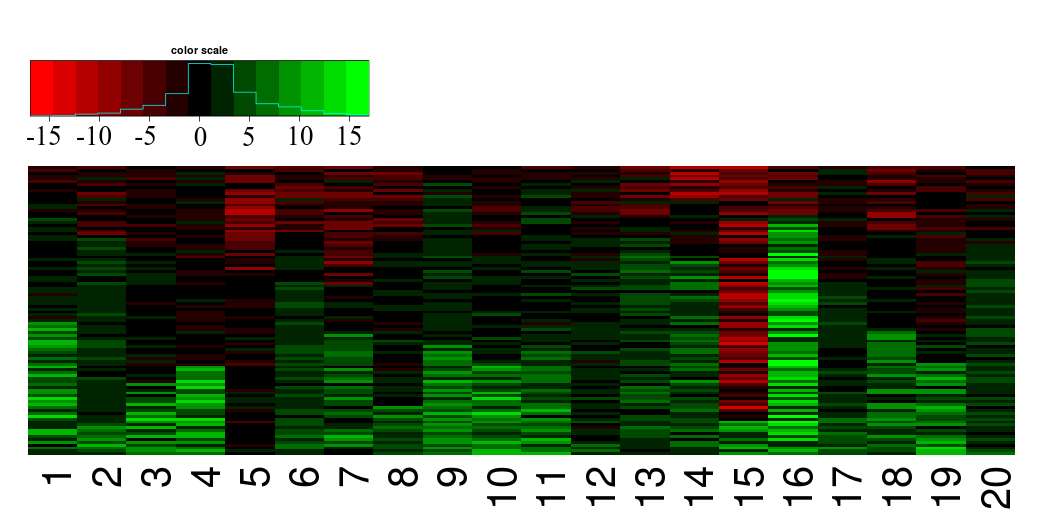
\includegraphics[scale = 0.3]{./veera/true_y_heatmap_sim_final.png}
        \caption{Simulated $y_{sg}$ ordered by true $e_{sg}$.}
        \vspace{0.5 cm}
    \end{subfigure}\\
    ~
    \begin{subfigure}[b]{0.98\textwidth}
        \centering
        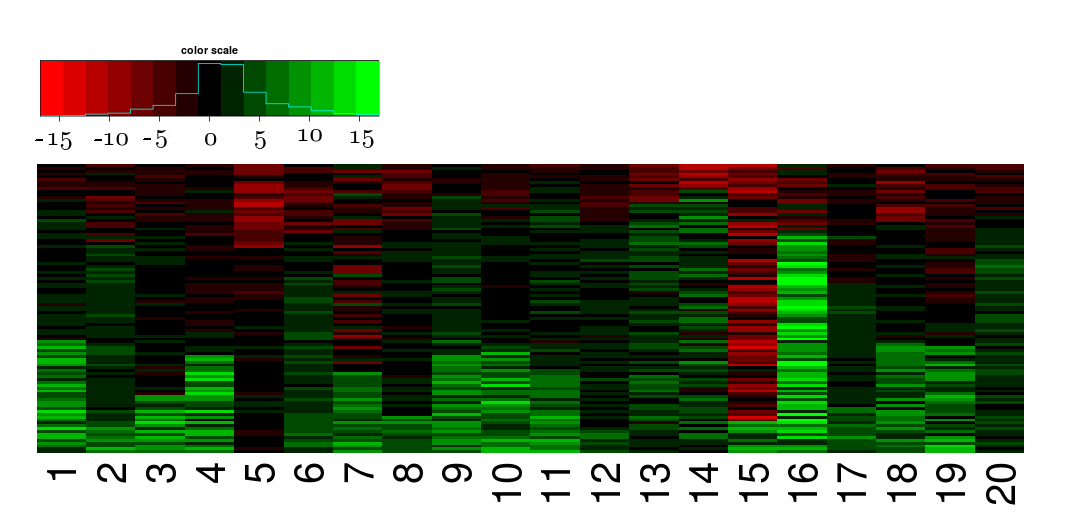
\includegraphics[scale = 0.3]{./veera/estimated_y_heatmap_sim_final.png}
        \caption{Simulated $y_{sg}$ ordered by estimated $e_{sg}$.}
        \vspace{0.5 cm}
    \end{subfigure}\\
    ~ 
    \begin{subfigure}[b]{0.98\textwidth}
        \centering
        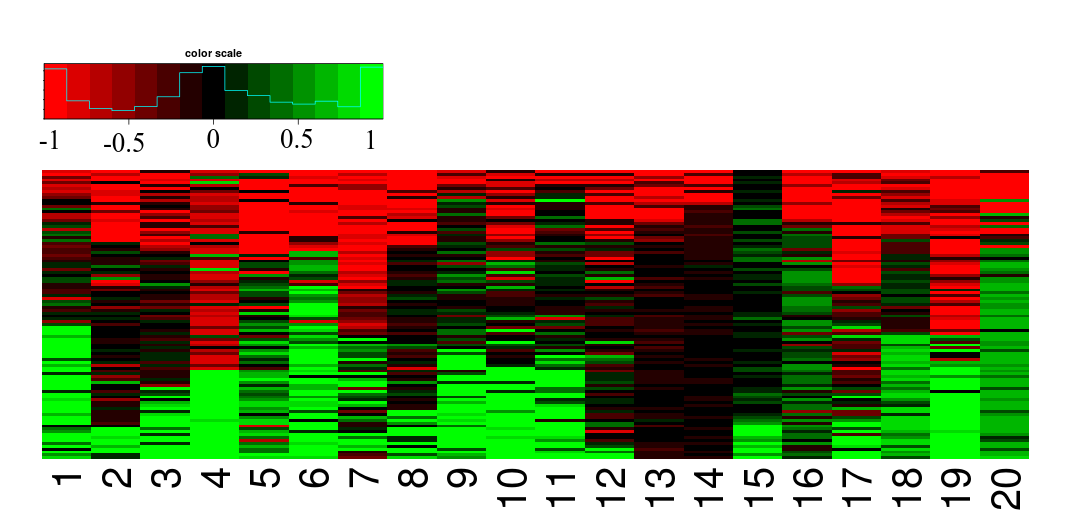
\includegraphics[scale = 0.3]{./veera/estimated_d_heatmap_sim_final.png}
        \caption{$d_{sg}$ ordered by true $e_{sg}$.}
	\vspace{0.5 cm}
    \end{subfigure}
    \caption{(a): Simulated data $y_{sg}$. Samples in each column are sorted by true $e_{sg}$. (b) Simulated data $y_{sg}$. Samples in each column are sorted by estimated $E\left( e_{sg} \mid \bfy \right)$. (c) Differences $d_{sg}=p^+_{sg} - p^-_{sg}$ with the same ordering as in panel (a). The ordering of samples change according to the protein (column) but is the same throughout the 3 panels.}
\label{fig:sim_poe_heatmap_1}
\end{figure}


%\begin{figure}[H]
%    \centering
%    \begin{subfigure}[b]{0.54\textwidth}
%        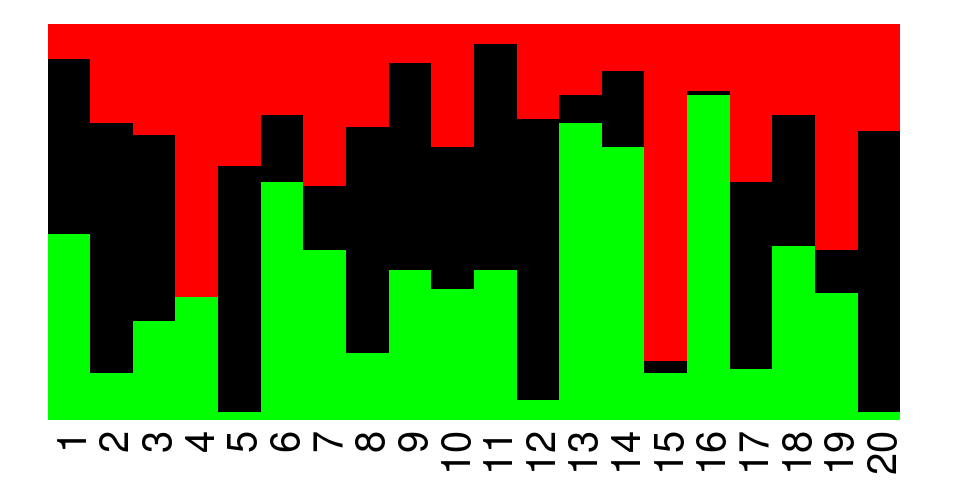
\includegraphics[scale = 0.25]{./veera/true_e_heatmap_sim.png}
%        \caption{Simulated $e_{sg}$.}
%    \end{subfigure}%
%    ~
%    \begin{subfigure}[b]{0.54\textwidth}
%        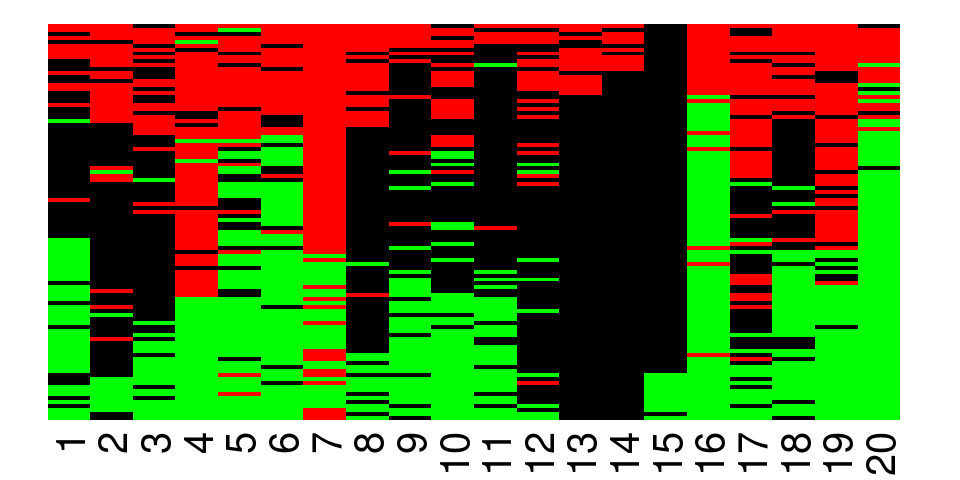
\includegraphics[scale = 0.25]{./veera/estimated_e_heatmap_sim.png}
%        \caption{Estimated $e_{sg}$.}
%    \end{subfigure}
%    \caption{(a) Simulation truth: $e_{sg}=1$ (green), $e_{sg}=0$ (black), $e_{sg}=-1$ (red).  (b) Point estimates of $e_{sg}$. Rows represent tumors (samples) while columns represent genes (proteins). Each column is ordered in a different way within each heatmap. The ordering of samples change according to the protein (column) but is the same throughout the 2 panels.}
%\label{fig:sim_poe_heatmap_2}
%\end{figure}


%\begin{figure}[H]
%\centering
%\includegraphics[scale=0.75]{./veera/mcmc_chains_sim.pdf}
%\caption{MCMC samples for the log-likelihood and for some of the marginals.}
%\label{fig:traces_poe}
%\end{figure} 

\begin{figure}[H]
\centering
\includegraphics[scale=0.7]{./veera/density_estimates_sim_subset.pdf}
\caption{Posterior density estimates. Vertical bars represent centralized gene expressions $y_{sg} - \mu_g - \alpha_s, \ s = 1, ..., S$ for all genes $g$ collored according to its estimated cluster membersip indicators (top) and true cluster membership indicators (bottom). Full lines represent the best fitting uniform and normal components of the mixture a posteriori multiplied by the respective weights. Dashed line corresponds to a kernel density estimate based on the vertical bars. Color code: black = -1, red = 0, green = 1.}
\label{fig:poe_densities}
\end{figure} 


\subsection{Simulation 2: nested partitions}

In this section we describe the simulation to validate inference on the NobLoc model. We replicated the scenario in \cite{lee2013}, with 100 samples and 20 proteins. The simulation truth incorporates the local clustering feature of first partitioning proteins and then within protein cluster, partitioning the samples. However, instead of simulating the protein and sample partitions according to a zero inflated Pólya urn, we fixed the partition of proteins upfront to have two active protein clusters, the first one containing  proteins with 3 active sample clusters; and the second containing 4 proteins with 2 active sample clusters. The cluster-membership assignment of samples was made uniformly at random among the available sample clusters. The cluster specific means were fixed at the same values in Table 1 of \cite{lee2013}. Inactive samples and proteins were all sampled from $Unif(-0.8, 0.8)$. The standard deviation of the Gaussian sampling model for active samples was fixed at $\sigma_g = 0.1$ For an illustration, see Figure \ref{fig:nobloc_sim_fit} panel (a). 

In Figure \ref{fig:nobloc_sim_fit} panel (b) we can see that the underlying cluster structure was reasonably captured by the NobLoc model. The only discrepancy is the inclusion of protein 19 in the first active cluster together with proteins 1 - 8, instead of classifying it as an inactive protein according to the simulation truth.

\begin{figure}[H]
\centering
\begin{subfigure}[b]{0.48\textwidth}
\includegraphics[scale=0.5]{./veera/true_heatmap_nobloc_sim.png} %\hspace{1cm}
\caption{Simulated $y_{sg}$ ordered by \\ true cluster assignments.}
\end{subfigure}
\begin{subfigure}[b]{0.48\textwidth}
\includegraphics[scale=0.5]{./veera/mcmc_heatmap_nobloc_sim.png}
\caption{Simulated $y_{sg}$ ordered by \\ estimated cluster assignments.}
%\vspace{0.5 cm}
\end{subfigure}
\caption{(a): Observations ordered according to the simulation truth. (b): Observations ordered according to estimated cluster membership indicators a posteriori. In both panels, rows represent samples while columns represent proteins.}
\label{fig:nobloc_sim_fit}
\end{figure} 


\section{Lung Cancer Dataset}

\subsection{The data}

The dataset consists of protein profiles coming from an RPPA experiment on lung cancer samples. The data records 233 proteins  that were pre-selected for their biological relevance to the study of this type of cancer. The data records samples from 687 patients and 124 cell lines. The objective is to identify groups of similar patients and cell lines with respect to subgroups of co-expressed proteins (we informaly say that proteins are co-expressed if their expressions are correlated). We therefore expect that the samples (patients and cell lines) can be partitioned in a different way depending on the group of co-expressed proteins that is considered. 

\subsection{Results}

We describe here the results of a joint inference of the POE model and nested clustering by NoB-LoC. We start by analyzing the results of directly applying the NoB-LC model to the original lung data (without running POE first), which is illustrated in Figure \ref{fig:nobloc_fit} (a).

\begin{figure}[H]
\centering
\includegraphics[scale=0.12]{./veera/all_heatmap_no_poe.png} \hspace{2cm}
\includegraphics[scale=0.12]{./veera/all_heatmap_after_poe.png}
\caption{Observed protein expression arranged according to posterior estimated cluster structure under NoB-Loc. Only active proteins are displayed. Panel (a) shows the result of application of the NobLoc model on the original data and panel (b) shows the results after the application of POE.}
\label{fig:nobloc_fit}
\end{figure} 

Figure \ref{fig:match_patients_cell_lines} shows one of the blocks in Figure \ref{fig:nobloc_fit} in more details highlighting the similarities between the cell lines and proteins in that block. Samples are reasonably homogeneous in terms of the expressions of the particular subgroup of proteins shown in the figure. Notice also that some proteins present typically high expression while others typically present low expression considering the particular group of samples.


\begin{figure}[H]
\centering
\includegraphics[scale=0.5]{./veera/zoom_after_poe_new.png}
\caption{Protein expressions within one of the samples/proteins blocks of Figure \ref{fig:nobloc_fit} (b). The cell lines and patients exhibit very similar profiles when considering the subset of proteins that were clustered together by the model.}
\label{fig:match_patients_cell_lines}
\end{figure} 

\section{Discussion and Future Directions}

Some innovations were introduced in this chapter: (i) The model naturally accounts for co-expression of genes and/or proteins in a manner that allows distinct clustering of samples depending on each estimated subgroup of co-expressed functional units or pathways; (ii) We develop efficient models for “matching” patients and cell line profiles. Development of such inferential tools is of critical relevance to implementing precision medicine, since it can be used for potential treatment assignment that is specific to a patient, and borrows information not only from that patient, but also from cell lines coming from external sources. The latter is critical also because experiments with cell lines can be carried out freely. (iii) Third, the approach does not need to be restricted to cell lines and patients but can be generalized to multiplatform omics profiles from diverse model systems such as patient-derived xenographs (PDX) models and organoids.

This chapter makes two important methodological contributions in Bayesian non-parametrics: (i) the seamless integration of the (modified) probability of expression (POE) model for noise reduction and the nested bi-clustering approach; (ii) the formal probabilistic modeling of co-clustering between cell lines and patients based on profile similarities via dependent priors on partition models.

There are some areas that need to be more thoroughly investigated. One of them is the need to extend the simulation studies where the underlying truth differs from the POE and NobLoc models in order to address the performance of the proposed methodology under model misspecification. In our results, we restricted the matching of cell lines and patients to a conditional zero inflated P\'olya urn (see section \ref{sec:nobloc_matching}), therefore the investigation of the other models for matching information from cell lines to patients is also proposed as a future work.

One of the limitations of the oroposed approach is the computational effort of full posterior simulation. Alternative implementations based on variational inference for example are possible alternatives (see section 1.4).

\chapter{Conclusions and future directions}
\label{ch:conclusions}

The common theme of the three major projects in this thesis was the
use of dependent priors for mixtures and random partitions. 
We discussed some motivating examples where the scientific research
questions naturally give rise to such dependent structures. 
Information on a specific form of dependence represents potentially
useful expert knowledge, which should be exploited when
available. It is still common practice, however, to ignore such domain
knowledge and proceed with default independent priors.
For the specific examples discussed in this thesis we constructed
suitable dependent models, developed practicable posterior inference
methods and demonstrated the proposed approaches in simulation studies
and in the actual applications.

Many open questions remain. For the application to cell lineage data,
the approach proposed in Chapter 3 can be characterized as an
empirical fit to the data with a model that respects the dependencies
that arise from the nature of the data. In future research we plan to
consider alternative generative models that mimick the actual biologic
process of how cells diversify. A generative model is used, for
example, in \cite{Shiffman18}, however still without using
restrictions and informative priors that would arise from the nature
of the data.

Also for the problem of matching patients and patient clusters with
representative cell lines that we considered in Chapter 4, many open
questions remain.
In the currently proposed model we match each patient cluster with one
representative cell line, implicitly allowing each cell line to be
paired with only one patient cluster. This restriction could be
removed, giving rise to a slightly different random structure.
Another aspect of the problem is that investigators have a preference
for reporting very distinct clusters of proteins (genes) and similarly
for the nested clusters of patients. That is, the desired summary of
the random partition should perhaps take into account preferences for
parsimony and interpretability. And such preferences could
alternatively already be included in the prior probability model.
One approach is the use of repulsive prior probability models that
favor very distinct clusters, for example the determinantal point
process (DPP) \citep{xu2016bayesian}. Similar issues arise with the applications in Chapters 2 and 3.







%\chapter{Making Tables and Including Figures}
\index{Making Tables and Including Figures@\emph{Making Tables
	and Including Figures}}%

The \emph{tabular} 
\index{commands!environments!tabular}%
environment allows us to create complex 
tables and figures, and draw boundaries around and within it.
The following example illustrates this:

\begin{table}[h]
\begin{center}
\caption{An example of a table.}
\vskip 10pt
\begin{tabular}{|ll|l|ll|l|lll|}
\cline{1-2} \cline{4-5} \cline{7-9}
\multicolumn{2}{|c|} {\textsl{Gegenwart}} & &
\multicolumn{2}{|c|} {\textsl{Imperfekt}} & &
\multicolumn{3}{|c|} {\textsl{Perfekt}} \\
\cline{1-2} \cline{4-5} \cline{7-9}
ich & bin  & & ich & war   & & ich & bin  & gewesen \\
du  & bist & & du  & warst & & du  & bist & gewesen \\
er  &      & & er  &       & & er  &      &         \\
sie & ist  & & sie & wart  & & sie & ist  & gewesen \\
es  &      & & es  &       & & es  &      &         \\
\cline{1-2} \cline{4-5} \cline{7-9}
wir & sind & & wir & waren & & wir & sind & gewesen \\
ihr & seid & & ihr & wart  & & ihr & seid & gewesen \\
sie & sind & & sie & waren & & sie & sind & gewesen \\
\cline{1-2} \cline{4-5} \cline{7-9}
Sie & sind & & Sie & waren & & Sie & sind & gewesen \\
\cline{1-2} \cline{4-5} \cline{7-9}
\end{tabular} \\[10pt]
Note: The assistance of Herr Professor Lothar Frommhold \\
in generating this table of German declensions \\
is gratefully acknowledged.
\vskip -20pt
\end{center}
\end{table}
\index{commands!environments!table}%

This table was created with the following sequence 
of commands:
\begin{verbatim}
\begin{table}[h]
\begin{center}
\caption{An example of a table.}
\vskip 10pt
\begin{tabular}{|ll|l|ll|l|lll|}
\cline{1-2} \cline{4-5} \cline{7-9}
\multicolumn{2}{|c|} {\textsl{Gegenwart}} & &
\multicolumn{2}{|c|} {\textsl{Imperfekt}} & &
\multicolumn{3}{|c|} {\textsl{Perfekt}} \\
\cline{1-2} \cline{4-5} \cline{7-9}
ich & bin  & & ich & war   & & ich & bin  & gewesen \\
du  & bist & & du  & warst & & du  & bist & gewesen \\
er  &      & & er  &       & & er  &      &         \\
sie & ist  & & sie & wart  & & sie & ist  & gewesen \\
es  &      & & es  &       & & es  &      &         \\
\cline{1-2} \cline{4-5} \cline{7-9}
wir & sind & & wir & waren & & wir & sind & gewesen \\
ihr & seid & & ihr & wart  & & ihr & seid & gewesen \\
sie & sind & & sie & waren & & sie & sind & gewesen \\
\cline{1-2} \cline{4-5} \cline{7-9}
Sie & sind & & Sie & waren & & Sie & sind & gewesen \\
\cline{1-2} \cline{4-5} \cline{7-9}
\end{tabular} \\[10pt]
Note: The assistance of Herr Professor Lothar Frommhold \\
in generating this table of German declensions \\
is gratefully acknowledged.
\vskip -20pt
\end{center}
\end{table}
\index{commands!environments!table}%
\end{verbatim}

The argument \texttt{h} indicates the position for the 
table, in this case ``here if possible''. Other values
of this argument are:
\texttt{t} (top of the page),
\texttt{b} (bottom of the page),
\texttt{p} (on the page of floats) and 
\texttt{H} (HERE! - requires using the package float.sty.
Note: When this option is used, LaTeX ignores all of its formatting
rules and does what you say, putting the entire float exactly where
it is defined. Check your output to make sure it is what you want!
If you are having trouble with LaTeX wanting to put a figure that's
larger than roughly half-a-page, as well as all of the figures
following it, at the end of a chapter, try using the command
\cn{clearpage} immediately following the large figure --- and maybe
a \cn{newpage} later.)
It is possible to combine several arguments, such as
\texttt{ht} (``here if possible, otherwise on top of
the page''). The default is \texttt{tbp}.

Figure \ref{f:ex} is a typical example of inclusion of a 
figure contained in an encapsulated PostScript file. 
\index{PostScript}%
\index{encapsulated PostScript}%
In order to use it, it is necessary to include the 
command \cn{usepackage\{psfig\}} 
\index{psfig}%
at the beginning of the document.

\begin{figure}[htb] % Imported eps example.
\begin{center}
\ \psfig{file=pup-on-rug.eps,height=1.5in,width=2.0in}
\caption{An example of an imported eps file.}
\label{f:ex}
\end{center}
\end{figure}
\index{commands!environments!figure}%
You can see the commands that generated this
figure in the source file. Look for the line
\cn{begin\{figure\}[htb] \% Imported eps example. }

The command that imports the file is \cn{psfig}, and it also 
controls its size (\texttt{height} and \texttt{width}), and 
can rotate the figure (\texttt{angle}).

Figures can also be drawn by using \LaTeX{} commands. 
Figure \ref{f:circuit} is an example 
(taken from \cite{gms:tlc}).

\begin{figure}[htb] % Picture example.
\begin{center}
   \setlength{\unitlength}{4mm}
   \begin{picture}(12,10)(-2,0)
      \linethickness{0.4pt}
      \qbezier(2.00,6.00)(7.00,6.00)(9.00,3.00)
      \qbezier(2.00,0.00)(7.00,0.00)(9.00,3.00)
      \qbezier(2.00,6.00)(4.00,3.00)(2.00,0.00)
      \qbezier(1.00,6.00)(3.00,3.00)(1.00,0.00)
      \put(9.75,3.00){\circle{1.50}}
      \put(10.50,3.00){\line(1,0){1.50}}
      \put(0.00,5.00){\line(1,0){1.50}}
      \put(0.00,1.00){\line(1,0){1.50}}
   \end{picture}
\caption{An example of a picture}
\label{f:circuit}
\end{center}
\end{figure}
\index{picture}%

The commands that generated this
picture are in the source file following the line
\cn{begin\{figure\}[htb] \% Picture example.  }

The commands used have rather obvious meanings. In particular, 
the command \cn{qbezier} 
\index{commands!qbezier@\cn{qbezier}}%
draws a quadratic Bezier curve, 
defined by its two ending points, and a third point (whose 
coordinates are in the middle) that is used as control point. 
Figure \ref{f:qb} illustrates the effect of the control point:

%\begin{figure}[htb] % Bezier curves example.
\begin{figure}[h] % Bezier curves example.
\begin{center}
   \setlength{\unitlength}{.8mm}
   \begin{picture}(55,55)(-15,0)
      \linethickness{1pt}
      \qbezier(0,0)(-10,30)(50,30)
      \qbezier(0,0)(20,50)(50,30)
      \thinlines
      \put(0,0){\line(-1,3){10}}
      \put(50,30){\line(-1,0){60}}
      \put(0,0){\line(2,5){20}}
      \put(50,30){\line(-3,2){30}}
      \put(0,0){\circle*{1}}
      \put(0,-1){\makebox(0,0)[t]{$A_{0,0}$}}
      \put(-10,30){\circle*{1}}
      \put(-10,31){\makebox(0,0)[b]{$B_{10,30}$}}
      \put(50,30){\circle*{1}}
      \put(58,29){\makebox(0,0)[b]{$C_{50,30}$}}
      \put(20,50){\circle*{1}}
      \put(20,51){\makebox(0,0)[b]{$D_{20,50}$}}
   \end{picture}
\caption{Bezier curves}
\label{f:qb}
\end{center}
\end{figure}
\index{Bezier curves}%


This figure has been generated with the following commands:
\begin{verbatim}
\begin{figure}[htb] % Bezier curves example.
\begin{center}
   \setlength{\unitlength}{.8mm}
   \begin{picture}(55,55)(-15,0)
      \linethickness{1pt}
      \qbezier(0,0)(-10,30)(50,30)
      \qbezier(0,0)(20,50)(50,30)
      \thinlines
      \put(0,0){\line(-1,3){10}}
      \put(50,30){\line(-1,0){60}}
      \put(0,0){\line(2,5){20}}
      \put(50,30){\line(-3,2){30}}
      \put(0,0){\circle*{1}}
      \put(0,-1){\makebox(0,0)[t]{$A_{0,0}$}}
      \put(-10,30){\circle*{1}}
      \put(-10,31){\makebox(0,0)[b]{$B_{10,30}$}}
      \put(50,30){\circle*{1}}
      \put(58,29){\makebox(0,0)[b]{$C_{50,30}$}}
      \put(20,50){\circle*{1}}
      \put(20,51){\makebox(0,0)[b]{$D_{20,50}$}}
   \end{picture}
\caption{Bezier curves}
\label{f:qb}
\end{center}
\end{figure}
\end{verbatim}



%\chapter{An Example of Mathematical Writing}
\index{An Example of Mathematical Writing%
@\emph{An Example of Mathematical Writing}}%

\section{Generalized Fatou's Lemma}
\index{Generalized Fatou's Lemma%
@\emph{Generalized Fatou's Lemma}}%

Here we show an application of the following lemma:

\begin{lem}[Generalized Fatou's Lemma] \label{l:fatou}

Let $A$ be a Dedekind ring and $F$ a rational series 
in $A[[X]]$, i.e., $F = p/q$ for some 
$p, q \in A[X]$. Then there exist two polynomials 
$P, Q \in A[X]$ such that $F = P/Q$, 
where $P$ and $Q$ are relatively prime and 
$Q(0) = 1$.

\end{lem}

\proof
See \cite{bertin:psn}, p.~15, theorem~1.3.
\endproof

\begin{thm} \label{l:req}
Let $\{c_n\}_{n=-\infty}^{\infty}$ a set of 
elements from $K$ such that $c_n \in k'$ for every 
$n \geq n_0$, and verifying the following recurrence 
relation of order M:
\begin{equation}
c_n\ =\ r_1\,c_{n-1} + r_2\,c_{n-2} + \dots + r_M\,c_{n-M}
\end{equation}
for every $n \in \mathbb Z$, where $r_1,r_2,\dots,r_M$ are in 
$K$, $r_M \neq 0$. 
Then:

\item{(i)} The coefficients $r_1,r_2,\dots,r_M$ are in 
$k'$, and for every $n \in \mathbb Z$, $c_n \in k'$.

\item{(ii)} If $c_n \in \mathcal O_{k',v}$ 
for every $n \geq n_0$, then the coefficients 
$r_1,r_2,\dots,r_M$ are all in 
$\mathcal O_{k',v}$.

\end{thm}


\proof 

\item{(i)} Let $C_n$ and $R$ be the matrices:

\begin{equation}
C_n\ =
\ \left(
\begin{array}{llll}
              c_n & c_{n+1} & \hdots & c_{n+M-1} \\
              c_{n+1} & c_{n+2} & \hdots  & c_{n+M} \\
              \vdots & \vdots & \ddots & \vdots \\
              c_{n+M-1} & c_{n+M} & \hdots & c_{n+2M-2}
\end{array}
\right)
\end{equation}
and
\begin{equation}
R\ =
\ \left(
\begin{array}{lllll}
              0 & 1 & 0 & \hdots & 0 \\
              0 & 0 & 1 & \hdots & 0 \\
             \vdots & \vdots & \vdots & \ddots & \vdots \\
              0 & 0 & 0 & \hdots & 1 \\
              r_M & r_{M-1} & r_{M-2} & \hdots & r_1 
\end{array}
\right)
\end{equation} 

We have that $C_{n+1} = R\,C_n$. Since the recurrence 
relation is of order M, $C_n$ is non singular. 
On the other hand, $R = C_{n+1}\,C_{n}^{-1}$. Since the 
elements of $C_n$ are in $k'$ for $n \geq n_0$, the entries 
of $R$, and those of $R^{-1}$, will be in $k'$. Since 
$C_{n-1} = R^{-1}\,C_n$, we get that the entries of 
$C_n$ will be in $k'$ also for $n < n_0$. 

\item{(ii)} For each $t \geq n_0$ define the formal 
power series 

\begin{equation}
F_t(X)\ =\ \sum_{n=0}^{\infty} c_{t+n}\,X^n
\end{equation}
which is in $\mathcal O_{k',v}[[X]]$. 
We have $F_t(X) = p_t(X)/q(X)$, 
where $p_t(X),q(X) \in k'[X]$ are the following:
\begin{equation}
p_t(X)\ =\ \sum_{j=0}^{M-1} \Bigl( c_{t+j} - 
                    \sum_{i=1}^{j} r_i\,c_{t+j-i} \Bigr)\,X^j
\end{equation}
\begin{equation}
q(X)\ =\ 1 - r_1\,X - r_2\,X^2 - \dots - r_M\,X^M
\end{equation}
This can be checked by multiplying $F_t(X)$ by $q_t(X)$ 
and using the recurrence relation, which gives 
$F_t(X)\,q(X) = p_t(X)$ (see \cite{poorten:sp}). 

Now we will prove that $p_t(X)$ and $q(X)$ are relatively 
prime. To do so, we will see that they cannot have any 
common root (in $\overline {k'}$). In fact, assume 
that $\alpha$ is a common root of $p_{t_0}(X)$ and $q(X)$ 
for some $t_0 \geq n_0$, i.e.: 
$p_{t_0}(\alpha) = q(\alpha) = 0$. 
Since $q(0)=1$, then $\alpha \neq 0$. Now we have:
\begin{equation}
X\,F_{t_0+1}(X) = F_{t_0}(X) - c_{t_0}
\end{equation}
so:
\begin{multline}
X\,p_{t_0+1}(X) = X\,q(X)\,F_{t_0+1}(X) \\
= q(X)\,(F_{t_0}(X) - c_{t_0}) = p_{t_0}(X) - c_{t_0}\,q(X)
\end{multline}
Hence $p_{t_0+1}(\alpha) = 0$, which means that $\alpha$ is 
also a root of $p_{t_0+1}(X)$. By induction we get that 
$p_t(\alpha) = 0$ for every $t \geq t_0$. Grouping the 
terms of $p_t(X)$ with respect to $c_t,c_{t+1},\dots,c_{t+M-1}$, 
we get:
\begin{equation}
p_t(X) = \sum_{j=0}^{M-1} a_j(X)\,c_{t+j}
\end{equation}
where 
\begin{equation}
a_j(X) = X^j\,\Bigl( 1 - \sum_{i=1}^{M-j-1} r_i\,X^i \Bigr)
\end{equation}
Note that $a_0(X),a_1(X),\dots,a_{M-1}(X)$ do not depend on t. 
On the other hand $p_t(\alpha)=0$ implies
\begin{equation}
\label{e:coldep}
\sum_{j=0}^{M-1} a_j(\alpha)\,c_{t+j} = 0
\end{equation}
for every $t \geq t_0$. Note that $a_{M-1}(\alpha)=\alpha^{M-1}
\neq 0$, so $a_0(\alpha),a_1(\alpha),\dots,a_{M-1}(\alpha)$ 
are not all zero, and (\ref{e:coldep}) means that the columns 
of the matrix $C_{t_0}$ are linearly dependent, so 
$\det C_{t_0}=0$, which contradicts the fact that $C_{t_0}$ 
is non singular. Hence, the hypothesis that $p_t(X)$ and 
$q(X)$ have a common root has to be false. This proves that 
$p_t(X)$ and $q(X)$ are relatively prime. 

By (generalized Fatou's) lemma~\ref{l:fatou}, 
and taking into account that 
$\mathcal O_{k',v}$ is a Dedekind ring, 
we get that there exist two relatively prime 
polynomials $P_t(X)$ and $Q_t(X)$ in 
$\mathcal O_{k',v}[X]$ such that 
$F_t(X) = P_t(X)/Q_t(X)$ and $Q_t(0)=1$. Hence: 
$p_t(X)\,Q_t(X) = q(X)\,P_t(X)$. By unique factorization 
of polynomials in $k'[X]$, there is a $u \in k'$ such that 
$P_t(X) = u\,p_t(X)$ and $Q_t(X) = u\,q_t(X)$. Since 
$Q_t(0)=q(0)=1$, we get that $u=1$, so 
$P_t(X) = p_t(X)$ and $Q_t(X) = q(X)$. 
Hence, the coefficients of $q(X)$ are in 
$\mathcal O_{k',v}$. 

\endproof


\section{Other Examples of Mathematical Writing}

\subsection{An Example of a Commutative Diagram}
\index{An Example of a Commutative Diagram%
@{An Example of a Commutative Diagram}}%

The following is an example of a commutative diagram.
\index{commutative diagram}%
It requires the \texttt{amscd} package.
\index{amscd package@{\texttt{amscd} package}}

\begin{equation*}
\newcommand{\End}{\operatorname{End}}
\begin{CD}
S^{{\mathcal{W}}_\Lambda}\otimes T   @>j>>   T\\
@VVV                                    @VV{\End P}V\\
(S\otimes T)/I                  @=      (Z\otimes T)/J
\end{CD}
\end{equation*}

That diagram has been made with the following commands:

\begin{verbatim}
\newcommand{\End}{\operatorname{End}}
\begin{CD}
S^{{\mathcal{W}}_\Lambda}\otimes T   @>j>>   T\\
@VVV                                    @VV{\End P}V\\
(S\otimes T)/I                  @=      (Z\otimes T)/J
\end{CD}
\end{verbatim}

\subsection{Using AMS Fonts}
\index{Using AMS Fonts@{Using AMS Fonts}}

To use AMS fonts it is necessary to choose from an assortment 
of \LaTeX{} packages. For instance the command 
\cn{usepackage\{amsfonts\}} calls in the \emph{amsfonts} package, 
which provides blackboard bold letters (e.g. $\mathbb{R}$) and 
some math symbols. A superset of that package is 
\emph{amssymb}. Other packages are \emph{eufrak} 
for Frankfurt letters (e.g. $\mathfrak{R}$)
and \emph{eucal} for Euler script 
(e.g. $\mathcal{R}$). 
Consult the \LaTeX{} documentation about this subject 
for additional information.



%%%%%%%%%%%%%%%%%%%%%%%%%%%%%%%%%%%%%%%%%%%%%%%%%%%%%%%%%%%%%%%%%%%%%%
% Appendix/Appendices                                                %
%%%%%%%%%%%%%%%%%%%%%%%%%%%%%%%%%%%%%%%%%%%%%%%%%%%%%%%%%%%%%%%%%%%%%%
%
% If you have only one appendix, use the command \appendix instead
% of \appendices.
%
\appendices
\index{Appendices@\emph{Appendices}}%



%\appendix 

\chapter{Probability distributions}
\label{appendix_A}

Here we describe the parameterization used for some of the probability distributions referred throughout the text. Namely: Gamma, Inverse Gamma, Exponential, Laplace, univariate and multivariate Student T (with location-scale parameters), univariate and multivariate Gaussian.

\section{Normal}

A continuous random variable $X$ follows a normal distribution $N(\mu, \sigma^2)$ if its density is

$$ f_X(x) = \frac{1}{\sqrt{2\pi}\sigma^2} \exp\left\{-\frac{1}{2}\left( \frac{x - \mu}{2\sigma}\right)^2\right\}, \ \ \ x \in \mathbb{R}.$$

It follows that $E(X) = \mu$ and $Var(X) = \sigma^2$.

\section{Multivariate Normal}

A continuous random vector $\bfX\in \mathbb{R}^d$ follows a $d-$variate normal distribution $N(\bfmu, \bfSigma)$ if its density is

$$f_{\bfX}(\bfx) = (2\pi)^{-\frac{d}{2}}\det|\Sigma|^{-\frac{1}{2}}\exp\left\{ -\frac{1}{2}(\bfX - \bfmu)^{\top} \bfSigma^{-1}(\bfX - \bfmu) \right\}, \ \ \ \bfx \in \mathbb{R}^d,$$

\noindent for $\bfSigma$ positive definite. It follows that $E(\bfX) = \bfmu$ and $Var(\bfX) = \bfSigma^2$.

\section{Gamma}

A continuous random variable $X$ follows a Gamma distribution $\mbox{Gama}(a,b)$ if its density is

$$f_X(x)=\frac{b^a}{\Gamma(a)}x^{a-1}e^{-bx}, \ \ \ x>0.$$

It folows that $E(X)=\frac{a}{b}$ and $Var(X)=\frac{a}{b^2}$.

\section{Inverse Gamma}

A continuous random variable $X$ follows an Inverse Gamma distribution with parameters $a$ and $b$, i. e.,  $X\sim GamaInv(a,b)$ if the random variable $Y = 1/X$ follows $Gamma(a, b).$ Then, $X$ has density

$$f_X(x)=\frac{b^a}{\Gamma(a)}x^{-a-1}e^{-\frac{b}{x}}, \ \ \ x>0.$$

It follows that $E(X)=\frac{b}{a-1}$ and $Var(X)=\frac{b^2}{(a-1)^2(a-2)}$.

\section{Student-t}

A continuous random variable $X$ follows a Stident T distribution with $\nu$ degrees of freedom, location $\mu$ and scale $\sigma$, if its density is

$$f_X(x)=\frac{\Gamma{\left(\frac{\nu+1}{2}\right)}}{\sigma\sqrt{\nu\pi}\Gamma(\frac{\nu}{2})}\left[\left(\frac{x-\mu}{\sigma}\right)^2+\nu\right]^{-\frac{\nu+1}{2}}, \ \ \ x\in \mathbb{R}.$$

In this case, we denote $X\sim T(\nu, \mu,\sigma)$. Under this parameterization, we have $E(X)=\mu$ if $\nu>1$ and $Var(X)=\sigma^2\times \frac{\nu}{\nu-2}$ for $\nu>2$. For $\nu = 1$, the average of the Student-T is not defined and if $\nu\leq 2$, the same holds for the variance.

\section{Multivariate Student-t}

A continuous random vector $\bfX \in \mathbb{R}^d$ follows a multivariate Student-T distribution with $\nu$ degrees of freedom and parameters $\bfmu$ and $\bfSigma$ if its density is

$$f_{\bfX}(\bfx)\propto\left[d+(\bfx-\bfmu)'\bfSigma^{-1}(\bfx-\bfmu)\right]^{-\frac{n+d}{2}} \ \ \ \bfx\in \mathbb{R}^d.$$

In this case, we denote $\bfX\sim T_n(\bfmu,\bfSigma)$. Here $\bfmu$ is the location parameter and the positive definite matrix $\bfSigma$ is the scale matrix. In this parameterization, $E(\bfX)=\bfmu$ if $\nu>1$ and $Var(\bfX)=\bfSigma\times \frac{\nu}{\nu-2}$ for $\nu>2$. Similar to the unidimensional case, $for \nu=1$ the mean of the distribution is not defined and if $\nu \leq 2$, the same happens for $\Sigma$.

An important result states that if $\bfX\sim T_n(\bfmu, \bfSigma)$, then the marginals are Student are also Student-T: $X_i \sim T_n(\mu_i, \sigma^2_i)$ where $\mu_i$ is the $i$-th entry of the mean vector and $\sigma^2_i=\bfSigma_{i,i}$.


\section{Laplace}

A continuous random variable $X \in \mathbb{R}^+$ follows a Laplace distribution with parameter $\lambda$, location $\mu$ and scale $\sigma>0$ if its density is


$$ f_X(x) = \frac{\lambda}{2\sigma}\exp\left\{ -\frac{\lambda |y - \mu |}{\sigma} \right\}, \ \ \ x > 0.$$

In this case, we denote $X \sim Laplace(\lambda, \mu, \sigma).$ It follows that $X \sim Laplace(\lambda, \mu, \sigma) \Rightarrow E(X) = \mu$ and $Var(X) = 2\sigma^2.$


\section{Negative Binomial}

A disctrete random variable $X$ follows a Negative Binomial distribution with parameters $n\in \mathbb{R}^{+}$ e $p \in (0,1)$ if $X$ its probability mass function

$$p_X(x)=\frac{\Gamma(x+n)}{\Gamma(x+1)\Gamma(n)}(1-p)^n p^x, \ \ \ x=0, 1, 2, \ldots$$

In this case, we denote $X\sim \mbox{NegBin}(n, p)$.

Under such parameterization, $E(X)=\frac{n p}{1-p}$ and $Var(X)=\frac{n p}{(1-p)^2}$.

\section{Log Normal}

A continuous random variable $X$ follows a $\mbox{LogNormal}(\mu, \sigma)$ distribution if the random variable $Y:=\log X$ follows a normal distribution $N(\mu, \sigma^2)$. In this case, the density function of $X$ is

$$f_X(x)=\frac{1}{x\sqrt{2\pi\sigma^2}}\exp\left\{-\left(\frac{\log x- \mu}{\sigma}\right)^2\right\}, \ \ \ x>0.$$

It follows that $E(X)=e^{\mu+\frac{\sigma^2}{2}}$ and $Var(X)=(e^{\sigma^2}-1)e^{2\mu+\sigma^2}$.


%\appendix 

\chapter{Appendix for Chapter 2}
\label{appendix_B}

\section{Full Conditionals}
\label{sec:full_cond}

We briefly describe the full conditional posterior distributions,
numbered (1) through (9) below, that define the transition
probabilities in the Gibbs sampler MCMC implementation. We define $\bfPsi:=(\bftheta, \bfy)$ as the random vector that includes the full parameter vector as well as the data, and we use the notation $\bfPsi_{-a}$ to represent $\bfPsi$ excluding component $a$.

\begin{enumerate}
\item {\bf Updating $v_{0u},$} $ u = 1, 2, 3$:
  \begin{multline*}
  (v_{0u} \mid \bfPsi_{-v_{0u}}) \sim \mbox{Gamma}\left(a_v + \frac{1}{2}CDL
  \times \kappa_{u}, \right.  \\
  \left. b_v + \frac{1}{2}\sum^C_{c=1} \sum^D_{d=1}
  \sum^L_{\ell=1} \sum^{\kappa_u}_{m=1}(\mu^*_{cd\ell u}(m) -
  \mu_{0u})^2\right).
  \end{multline*}

\item {\bf Updating $\mu_{0u},$} $u = 1, 2, 3$:
  \begin{multline*}
  (\mu_{0u} \mid \bfPsi_{-\mu_{0u}}) \sim N\left(\frac{ v_{0u}\sum^C_{c=1}
  \sum^{D}_{d=1} \sum^L_{\ell=1} \sum^{\kappa_{u}}_{m=1} \mu^*_{cd\ell
    u}(m) + \mu_{00}v_{00} }{ v_{00} + CDL \times \kappa_{u} v_{0u} },
  \right. \\
  \left. \frac{1}{ v_{00} + CDL \times \kappa_{u} v_{0u} }\right).$$
\end{multline*}

\item {\bf Updating $\mu^*_{cd \ell u}$: }
From equation (1), the vector $\bfmu_{cd\ell i}$ can be written as
$$
\bfmu_{cd\ell i} = \mu^*_{cd\ell 1}\left(\delta^1_{cdi}\right)\bfu_1 +
\mu^*_{cd\ell 2}\left(\delta^2_{cdi}\right)\bfu_2 + \mu^*_{cd\ell
  3}\left(\delta^1_{cdi}\right)\bfu_3,
$$
where
$\bfu_1 = (1, \ldots, 1, 0, \ldots, 0)^{\top}$,
$\bfu_2 = (0, \ldots, 0, 1, \ldots, 1, 0, \ldots, 0)^{\top}$
           and
$\bfu_3 = (0, \ldots, 0,\\ 1, \ldots, 1)^{\top}$
with 1's in positions $1,\ldots,\tau^1_{cd\ell}$ (for $\bfu_1$),
in positions $\tau^1_{cd\ell}+1 \ldots \tau^2_{cd\ell}$ (for $\bfu_2$) and
in position $\tau^2_{cd\ell} + 1 \ldots T$ (for $\bfu_3$), respectively.
We find that $(\mu^*_{cd\ell 1}(m) \mid \bfPsi_{-\mu^*_{cd\ell 1}(m)}) \sim N(a_1, b_1)$, with
$b_1 = (v_{01} + J (\#\mathcal{P}^m_{cd1}) \bfu_1^{\top}\bfSigma^{-1}_c
\bfu_1)^{-1}$
and
\begin{multline*}
  a_1 = b_1\, \left[\left(\sum_{i \in \mathcal{P}^m_{cd1}}\sum_j
    \bfy_{cd\ell ij} - J\bfu_2
    \sum_{i \in  \mathcal{P}^m_{cd1}}\mu^*_{cd\ell 2}(\delta^2_{cdi}) -
    J(\#\mathcal{P}^m_{cd1}) \bfu_3 \mu^*_{cd\ell 3}(m) \right)^{\top} \right. \\
    \left.\vphantom{\sum_{i \in  \mathcal{P}^m_{cd1}}} \bfSigma^{-1}_c \bfu_1 + \mu_{01}v_{01} \right],
\end{multline*}
    
  where $\mathcal{P}^m_{cd1} := \{1\leq i \leq I: \delta^1_{cdi} = m \}.$\\
Similarly, $(\mu^*_{cd \ell 2}(m) \mid \bfPsi_{- \mu^*_{cd \ell 2}(m)}) \sim N(a_2, b_2)$, with \\
$  b_2 =(v_{02} + J (\#\mathcal{P}^m_{cd2})
\bfu_2^{\top}\bfSigma^{-1}_c \bfu_2)^{-1}$ and

\begin{multline*}
a_2 = b_2\, \left[\left(
  \sum_{i \in \mathcal{P}^m_{cd2}} \sum_j \bfy_{cd\ell ij} - J\bfu_1
  \sum_{i \in \mathcal{P}^m_{cd2}}\mu^*_{cd\ell 1}(\delta^1_{cdi}) 
  - J\bfu_3
  \sum_{i \in \mathcal{P}^m_{cd\ell 2}}\mu^*_{cd \ell 3}(\delta^1_{cdi})\right)^{\top}\left.\\
     \left. \vphantom{\sum_{i \in \mathcal{P}^m_{cd2}} \sum_j}\bfSigma^{-1}_c \bfu_2 + \mu_{02}v_{02}\right], 
\end{multline*}

where $\mathcal{P}^m_{cd2} := \{1\leq i \leq I: \delta^2_{cdi} = m \}$.\\
And $(\mu^*_{cd \ell 3}(m) \mid \bfPsi_{-\mu^*_{cd \ell 3}(m)}) \sim N(a_3, b_3)$, with \\
$b_3 = (v_{03} + J (\#\mathcal{P}^m_{cd1}) \bfu_3^{\top}\bfSigma^{-1}_c
\bfu_3)^{-1}$ and

\begin{multline*}
  a_3 = b_3\, \left[\left( \sum_{i \in \mathcal{P}^m_{cd1}} \sum_j \bfy_{cd\ell ij} - J\bfu_2 \sum_{i \in \mathcal{P}^m_{cd1}}\mu^*_{cd\ell 2}(\delta^2_{cdi}) - J(\#\mathcal{P}^m_{cd1})\bfu_1 \mu^*_{cd\ell 1}(m) \right)^{\top} \right.\\
\left. \vphantom{\sum_{i \in \mathcal{P}^m_{cd2}} \sum_j}    \bfSigma^{-1}_c\bfu_3 + \mu_{03}v_{03}\right].
\end{multline*}
%
\item {\bf Updating $\bfSigma_c$: }
Under the normal-inverse Wishart conjugate model we get
\begin{multline*}
(\bfSigma_c \mid \bfPsi_{-\bfSigma_c}) \sim IW\left( IDLJ + \nu_{\Sigma}, \vphantom{\sum^J_{j=1}}\right. \\
\left. \sum^I_{i=1} \sum^D_{d=1} \sum^L_{\ell=1}
\sum^J_{j=1}(\bfy_{cdi\ell j} - \bfmu_{cd\ell i} )(\bfy_{cdi\ell j} -
\bfmu_{cd\ell i} )^{\top} + V_{\Sigma_c} \right)
\end{multline*}
%
\item {\bf Updating $\gamma$: }
\begin{multline*}
  (\gamma \mid \bfPsi_{-\gamma}) \sim \mbox{Beta}\left( a_{\gamma} + \sum^C_{c=1}
  \sum^D_{d=1} \sum^I_{i=1} \mathds{1}(\delta^2_{cdi} = \delta^1_{cdi}),
 \right. \\ 
  \left. b_{\gamma} + 
  \sum^C_{c=1} \sum^D_{d=1} \sum^I_{i=1} \mathds{1}(\delta^2_{cdi} \neq
  \delta^1_{cdi} ) \right)
\end{multline*}
%
\item {\bf Updating $\tau^1_{cd\ell}$ and $\tau^2_{cd\ell}$: }
We update $\tau^1_{cd\ell}$ and $\tau^2_{cd\ell}$ in different blocks of
the Gibbs sampler. This way we evaluate fewer scenarios than in the
case of sampling both together in a single step, due to the
restriction $\tau^1_{cd\ell}<\tau^2_{cd\ell}$.
\begin{gather}
 p(\tau^1_{cd\ell} \mid \bfPsi_{-\tau^1_{cd\ell}} ) \propto \prod^I_{i=1}
 \prod^J_{j=1} N(\bfy_{cd\ell ij}; \bfmu_{cd\ell i}, \bfSigma_c), \ \ \
 \tau^1_{cd\ell}<\tau^2_{cd\ell}. \nonumber \\
 p(\tau^2_{cd\ell} \mid \bfPsi_{-\tau^2_{cd\ell}} ) \propto \prod^I_{i=1}
 \prod^J_{j=1} N(\bfy_{cd\ell ij}; \bfmu_{cd\ell i}, \bfSigma_c), \ \ \
 \tau^1_{cd\ell}<\tau^2_{cd\ell}.
 \label{eq:tau}
\end{gather}
If evaluating the probabilities in \eqref{eq:tau} is too
computationaly intensive, one can alternatively implement
a Metropolis-Hastings transition probability, proposing 
% for sampling from each conditional proposing
unit increments or decrements, subject to the constraint
$\tau^1_{cd\ell}<\tau^2_{cd\ell}$. This would require at most
four evaluations of the right hand side product in \eqref{eq:tau}.  \ech

\item {\bf Updating cluster membership indicators $\delta^1_{cdi}$: }
  If $\delta^2_{cdi}\leq \kappa_1$, then $\delta^1_{cdi}$ is equal to the value of
  $\delta^2_{cdi}$ with probability 1. Otherwise, by multinomial-Dirichlet
  conjugacy results, the full conditional distribution of
  $\delta^1_{cdi}$ is
  $
  P(\delta^1_{cdi} =m \mid \bfPsi_{-\delta^1_{cdi}}) \propto
  \NN^1_{cdi}(m)\pi^1_{m}$, 
  $m=1,\ldots,\kappa_1$ 
%         \sim \mbox{Multinomial}\left((1, \ldots, \kappa_1); \ \ \
% (, \ldots,
%   \NN^1_{cdi}(\kappa_1)\pi_{1
%     \kappa_1})/\sum^{\kappa_1}_{m=1}\NN^1_{cdi}(m)\pi_{1m}\right),
%   $$
where $\NN^1_{cdi}(m)=\prod_{\ell} \prod_j N(\bfy_{cd\ell ij} \mid
\bfmu_{cd\ell i}, \bfSigma_c )$ with $\bfmu_{cd\ell i}$ evaluated under
$\delta^1_{cdi}=m$. 
%
\item {\bf Updating cluster membership indicators $\delta^2_{cdi}$: }
The full conditional p.m.f. for $\delta^2_{cdi}$ is given by
\begin{equation*}
P(\delta^2_{cdi} = m \mid \bfPsi_{-\delta^2_{cdi}}) \propto
\begin{cases}
  \gamma \times \NN^2_{cdi}(\delta^1_{cdi} )
  %{ \gamma  \NN^2_{cdi}(\delta^1_i ) + (1-\gamma) \sum^{\kappa_2 -
  %\kappa_1}_{m=\kappa_1+1} \pi^2_{m-\kappa_1}\NN^2_{cdi}(m) }, \ \ \
  & \mbox{ if } m =  \delta^1_{cdi}.\\ 
  (1-\gamma) \times \pi^2_{m-\kappa_1}  \NN^2_{cdi}(m)
  % { \gamma \NN^2_{cdi}(\delta^1_i) + (1-\gamma) \sum^{\kappa_2 -
  %   \kappa_1}_{m=\kappa_1+1} \pi_{2, m-\kappa_1}\NN^2_{cdi}(m)},   \ \ \ 
  & \mbox{ if } \kappa_1+1\leq m \leq \kappa_2.
\end{cases}
\end{equation*}
where $\NN^2_{cdi}(m)=\prod_{\ell} \prod_j
N(\bfy_{cd\ell ij} \mid \bfmu_{cd\ell i}, \bfSigma_c )$ with $\bfmu_{cd\ell
i}$ being calculated assuming $\delta^2_{cdi}=m$. 
%
\item {\bf Updating $\bfpi_{1}$ and $\bfpi_2$: }
under the conjugate multinomial-Dirichlet model we
find the following posterior distribution.
Let 
$n^1_m = \sum^C_{c=1} \sum^D_{d=1} \\ \sum^I_{i=1}
\mathds{1}(\delta^1_{cdi}=m)$. 
for $m=1, \ldots, \kappa_1$.
Similarly, let 
$n^2_m = \sum^C_{c=1} \sum^D_{d=1}$ $\sum^I_{i=1} \mathds{1}(\delta^2_{cdi}=m)$ for 
$m=\kappa_1+1,\ldots,\kappa_1+\kappa_2$.
Then $
  (\bfpi_1 \mid \bfPsi_{-\bfpi_1}) \sim \Dir(\eta_{11}     +n^1_1,\ldots,
                               \eta_{1\kappa_1}+n^1_{\kappa_1})
$
and
%   \mbox{Dirichlet}\left( \eta_{11} +
% , \ \ldots\  \right. \\
%   &\hspace{5 cm} \left. \ \ldots \ , \ \eta_{1 \kappa_1} + \sum^C_{c=1} \sum^D_{d=1} \sum^I_{i=1} \mathds{1}(\delta^1_{cdi}=\kappa_1) \right).
$
(\bfpi_2 \mid \bfPsi_{-\bfpi_2}) \sim \Dir(\eta_{21}+n^2_{\kappa_1+1}, \ldots, 
                     \eta^2_{\kappa_2-\kappa_1} +n^2_{\kappa_1+\kappa_2}). 
$

% \begin{align*}
%   (\bfpi_2 \mid \ldots) &\sim \mbox{Dirichlet}\left( \eta_{21} + \sum^C_{c=1} \sum^D_{d=1} \sum^I_{i=1} \mathds{1}(\delta^2_{cdi}=1 + \kappa_1),  \ \ldots \ \right. \\
%   &\hspace{5 cm} \left. \ \ldots \ , \ \eta_{2, \kappa_2 - \kappa_1} + \sum^C_{c=1} \sum^D_{d=1} \sum^I_{i=1} \mathds{1}(\delta^2_{cdi}=\kappa_2) \right) .
% \end{align*}
\end{enumerate}


\section{Number of Model Parameters for AIC and BIC}
\label{sec:number_param}

Here we describe how the number of parameters was determined when
evaluating the BIC criterion in sections 4 and 5 and
AIC in section 4. The description focuses on BIC, but
the same arguments are valid for evaluation of AIC. 

The number of parameters for a given model is a function of $\kappa_1$ and
$\kappa_2$ that can be decomposed as $N(\kappa_1, \kappa_2) = f( \kappa_1,
\kappa_2) + const$, where $const$ depends on the number of data points,
but not on $\kappa_1$ or $\kappa_2$. 
The only parameters in the likelihood that vary in number as $\kappa_1$ and
$\kappa_2$ change are
$\{\bfmu^*_{\ell ,u}: c\in [C], d\in [D], \ell \in [L], u \in [3] \}$,
which contains
$f(\kappa_1, \kappa_2) = CDL(2\kappa_1 + \kappa_2)$ parameters.
Therefore, $BIC = 2 \log p(\bfy \mid \theta) 
- N(\kappa_1, \kappa_2) \log n,$ where $n$ is the number of observations,
hence the comparison of any pair of models is invariant with respect to
the term $const$ and we can, for simplicity, consider $N(\kappa_1,
\kappa_2) = CDL(2\kappa_1 + \kappa_2)$.



%\appendix 

\chapter{Appendix for Chapter 3}
\label{appendix_C}

\section{Proper Prior on $(\bfmu_1, \ldots, \bfmu_k, b_1, \ldots, b_k, k)$}
\label{sec:proper_prior}

Here we show that $p(\bfmu_1, \dots, \bfmu_k, \bfb, k)$ defined in \eqref{eq:prior1} is a proper prior. In fact, since 

$$ \exp\left\{- \alpha \sum_{j=1}^k d(\bfmu_j, \bfmu_{b_j}) \right\}<1, \ \ \ \ \forall \ 1 \leq j \leq k,$$

\noindent it follows that

$$Z_k \leq \int \dots \int_{\mathbb{R}^{p \times k}} \prod_{j=1}^k \left[ p(\bm{\mu}_j)\right]k^k \ d\bfmu_1 \dots  d\bfmu_k = k^k < \infty.$$

\noindent Without loss of generality, we can truncate $P(k)$ to have suport $1\leq k \leq M$ for some finite upper limit $M$ and therefore $p(k)$ will be also proper. The truncation is justified in practical appications since one expects finite number of nodes in the tree.


\section{Full Conditional Distributions for the s-MST Model}
\label{sec:app_smst}

We now describe posterior inference under the s-MST model of Section \ref{sec:soft_mst}. A simple MCMC can be implemented in such a scenario, leading to the Gibbs sampling transition probabilities:
\begin{enumerate}
\item Updating $c_i$:
\begin{align*}
p (c_i = k | \bm{y}_i, \bfmu_k, \Sigma, w_k) &\propto L(\bm{y}_i | c_i = k, \bfmu_k, \Sigma) \ p(c_i = k | w_k)
\\
&\propto w_k \ \mathcal{N} (\bm{y}_i; \bfmu_{k}, \Sigma), \quad \forall k = 0, \dots, k.
\end{align*}

\item Updating $\bm{w}$:
\begin{align*}
p(\bm{w} | c_1, \dots, c_n) &\propto p(c_1, \dots, c_n | \bm{w}) \ p(\bm{w})
\\
&\sim \mbox{Dirichlet} (n_0 + \delta, \dots, n_k + \delta).
\end{align*}

%\item Updating $\Sigma_k, \forall k = 0, \dots, K$:
%\begin{align*}
%p (\Sigma_k | Y ,  \mbox{rest}) &\propto L(Y | c_1, \dots, c_n,  \bfmu_k, \Sigma_k) \ p(\Sigma_k)
%\\
%&\propto \prod_{i : c_i = k} \left\{ |\Sigma_k|^{-\frac{1}{2}} e^{-\frac{1}{2} (\bm{x}_i - \bfmu_k)^T \Sigma_k^{-1} (\bm{x}_i - \bfmu_k)} \right\} |\Sigma_k|^{- \frac{\nu + p + 1}{2}} e^{ - \frac{1}{2} \mbox{tr} (R \Sigma_k^{-1})}
%\\
%&\sim \mathcal{IW} \left( \nu + n_k, \Psi + \sum_{i : c_i = k} (\bm{y}_i - \bfmu_k)(\bm{y}_i - \bfmu_k)^T \right).
%\end{align*}
%In the case of unique covariance matrix $\Sigma$, we use all data points to update the parameters, obtaining $p (\Sigma | Y ,  \mbox{rest}) \sim \mathcal{IW} \left( \nu + n, \Psi + \sum_{i} (\bm{y}_i - \bfmu_k)(\bm{y}_i - \bfmu_k)^T \right)$.

\item Updating $\Sigma$:
\begin{align*}
p (\Sigma | Y ,  \mbox{rest}) &\propto L(Y |  \bfmu_k, c_1, \dots, c_n, \Sigma) \ p(\Sigma)
\\
&\propto \prod_{i=1}^n \left\{ |\Sigma|^{-\frac{1}{2}} e^{-\frac{1}{2} (\bm{x}_i - \bfmu_{c_i})^T \Sigma^{-1} (\bm{x}_i - \bfmu_{c_i})} \right\} |\Sigma|^{- \frac{\nu + p + 1}{2}} e^{ - \frac{1}{2} \mbox{tr} (R \Sigma^{-1})}
\\
&\sim \text{Inv-Wishart} \left( \nu + n, \Psi + \sum_{i} (\bm{y}_i - \bfmu_{c_i})(\bm{y}_i - \bfmu_{c_i})^T \right).
\end{align*}


\item Updating $\bfmu_k, \forall k = 1, \dots, k$:
\begin{align*}
p (\bfmu_k | Y, \mbox{rest}) &\propto L(Y | c_1, \dots, c_n,  \bfmu_k, \Sigma) \ p(\bfmu_j | \bfmu^{(-j)}, \bfb, \alpha, k)
\\
&\sim \mathcal{N} \left((\Sigma_p^{-1} + n_j \Sigma^{-1})^{-1} \left[\Sigma_p^{-1} \bfmu_p + \Sigma^{-1} \sum_{i:c_i = j} \bfy_i \right] , \\
&\left. \hspace{6 cm}(\Sigma_p^{-1} + n_j \Sigma^{-1})^{-1} \vphantom{ \sum_{i:c_i = j}} \right),
\end{align*}
where $f_j, \bfmu_p, \Sigma_p$ were defined in equations \eqref{eq:mu_cond_eucl1} and \eqref{eq:mu_cond_eucl2}.


\item Updating the branching structure: by resampling it from the prior conditionals $p(b_j = i | \bfmu_0, \dots, \bfmu_k, \bfb^{(-j)},  k)$ described in \eqref{eq:b_cond}.

%\item Updating the hyperparameter $\alpha$. We can use a Gamma prior (or Exponential), getting posterior conjugacy, i.e. 
%$$p(\alpha | \bfmu_0, \dots, \bfmu_K, \bfb, K) \sim \text{Gamma} \left(a_\alpha, b_\alpha + \sum_{j=1}^K d(\bfmu_j, \bfmu_{b_j}) \right)$$
%\textbf{This full conditional is still problematic because values of $\alpha$ too small are sampled. This, in turn, implies the sampling of trees that are not repulsive MST.}

\item Updating the dimension $K$ using a RJ-MCMC move:
\begin{enumerate}
\item Generate a proposal $\tilde{k} \sim q(\tilde{k} | k)$ and a matching set of parameters $\tilde{\bm{\theta}}_{\tilde{k}} \sim p_1(\tilde{\bm{\theta}}_{\tilde{k}} | y^\prime)$ as described in Section \ref{sec:mst_inference}
}
\item Accept $(\tilde{k}, \tilde{\bm{\theta}}_{\tilde{k}})$ with probability $\alpha$ defined in \eqref{eq:alpha}.
\end{enumerate}
\end{enumerate}

\section{Full Conditional Distributions for the h-MST Model}
\label{sec:app_hmst}

First, we list the full conditional distributions for implementation of Gibbs sampler on the model described in Section \ref{sec:model2_mst} conditionaly on the dimension $k$.

\begin{enumerate}

\item Updating $c_j$:

\begin{align*}
p (c_i = j | \bm{y}_i, \bfmu_j, \Sigma_j, w_j, k) &\propto L(\bm{y}_i | c_i = j, \bfmu_j, \Sigma) \ p(c_i = j | w_j)
\\
&\propto w_j \ \mathcal{N} (\bm{y}_i; \bfmu_{j}, \Sigma_j), \quad \forall j = 0, \dots, k.
\end{align*}

\item Updating $\bm{w}$:
\begin{align*}
p(\bm{w} | c_1, \dots, c_n, k) &\propto p(c_1, \dots, c_n | \bm{w}, k) \ p(\bm{w} \mid k)
\\
&\sim \mbox{Dirichlet} (n_0 + \delta, \dots, n_k + \delta).
\end{align*}

%\item Updating $\lambda_{jd}$:
%\begin{align*}
%p(\lambda_{jd} \mid \bfy, \bfmu, \Sigma, \bfc, k) &\propto \prod_{i \in S_j}%p(\bfy_i \mid \bfmu_j, \Sigma_j, c_i, k) p(\lambda_jd)\\
%& \sim \mbox{InvGamma}\left( \frac{\#S_j}{2} + a, \ \frac{1}{2} \sum_{i \in S_j}(y_i - \bfmu_j)^T\bfe_d\bfe_d^{\top}(y_i - \bfmu_j) + b\right),
%\end{align*}

%\noindent where $S_j := \{i: \ c_i=j\}$ and $\bfe_d$ denotes the $d$-th eigenvalue of $\Sigma_j$ (which is also the $d$-th column of $\bfE$).

\item Updating $\Sigma^{-1}$

\begin{align*}
p(\Sigma^{-1} \mid \bfy, rest) &\propto \prod^n_{i=1} p(\bfy_i \mid \bfmu_{c_i}, \Sigma^{-1})p(\Sigma^{-1})\\
&\sim Wishart \left( n + \nu, \left[ \Psi^{-1} + \sum^{n}_{i}(\bfy_i - \bfmu_{c_i})(\bfy_i - \bfmu_{c_i})^{\top} \right]^{-1}\right).
\end{align*}

\item Updating $\bfmu_j$:

The conditional posterior density $p(\bfmu_j\mid \bfy, \mbox{rest})$ is not straightforward to either write in analytic form or to sample from. 

Denote by $S_j:=\{i: \ c_i=j\}$ the set of observations that belong to cluster $j$. Combining the likelihood with the h-MST prior, we have

\begin{align*}
p(\bfmu_j \mid \bfmu^{(-j)}, \bfy, rest)&\propto \left[\prod_{i\in S_j} N(\bfy_i; \bfmu_{j}, \Sigma) N(\bfmu_j; \bfm, \sigma^2_0I)\right]\times \\
& \hspace{3 cm}\times\exp\left\{-\alpha\mathcal{W}( MST(\bfmu_1, \cdots, \bfmu_k) ) \right\},
\end{align*}

\noindent in which the sum $\mathcal{W}( MST(\bfmu_1, \cdots, \bfmu_k) )$ involves different terms depending on the position of $\bfmu_j$ in $\mathbb{R}^D$. This leads to the full conditional being a finite mixture of truncated normals, with non-overlapping truncation regions $A_l\subset \mathbb{R}^D, \ l=1, \ldots, n$ such that the neighbors of any node $\bfmu_j\in A_l$ are the same under the $MST(\bfmu_1, \ldots, \bfmu_k)$ when we fix the remaining nodes $\bfmu^{(-j)}$. The challenge lies in defining the regions $A_l$ that partition $\mathbb{R}^D$.

However, we can build a tractable and efficient Metropolis Hastings proposal $q(\tilde{\bfmu}_j \mid \bfmu_j; \bfmu^{(-j)}, \bfy, rest)$ to approximate $p(\bfmu_j\mid \bfy, \mbox{rest})$. We will omit the dependence on variables other than $\bfmu_j$ from the notation for clarity of exposition, therefore writing $q(\tilde{\bfmu}_j \mid \bfmu_j)$ instead of $q(\tilde{\bfmu}_j \mid \bfmu_j; \bfmu^{(-j)}, \bfy, rest)$. We define $q(\tilde{\bfmu}_j \mid \bfmu_j)$ as follows. Take from the edges $E_{\bfmu_1, \ldots, \bfmu_k}$ of the $MST(\bfmu_1, \ldots, \bfmu_k)$  the subset $V_j=\{i: \ \{j,i\} \in E_{\bfmu_1, \ldots, \bfmu_k} \}$ of all neighbors of node $j$. We propose a new component specific mean $\tilde{\bfmu}_j$ from


\begin{align*}
q(\tilde{\bfmu}_j \mid \bfmu_j)\propto \prod_{i\in S_j} N(\bfy_i; \tilde{\bfmu}_{j}, \Sigma) N(\tilde{\bfmu}_j; \bfm, \sigma^2_0I) \exp\left\{-\alpha\sum_{i \in V_j} d^2(\bfmu_i, \tilde{\bfmu}_j) \right\},
\end{align*}

\noindent which simplifies to $q(\tilde{\bfmu}_j \mid \bfmu_j)\sim N(\tilde{\bfmu_j}; \ \bfa_j, \bfB_j),$ where \ $\bfB_j = ( |S_j| \Sigma^{-1} +$ $\sigma^{-2}_0 I + 2\alpha |V_j|I )^{-1}$ and \ $\bfa_j = \bfB_j\left( \Sigma^{-1} \sum_{i \in S_j}\bfy_i + \sigma^{-2}_0\bfm + 2\alpha\sum_{l \in V_j}\bfmu_l\right).$ By denoting the proposed neighborhood of $\tilde{\bfmu}_j$ as $\tilde{V}_j=\{i: \{i,j\} \in E_{\bfmu^*_1, \ldots, \bfmu^*_k}\}$ where $\bfmu^*_l = \bfmu_l$ if $l\neq j$ and $\bfmu^*_j = \tilde{\bfmu}_j$, the resulting Metropolis Hastings acceptance probability equals 1 if $\tilde{V}_j = V_j$ and

\begin{align*}
\alpha&( \tilde{\bfmu}_j \mid \bfmu_j) = \min\left\{ 1, \frac{q(\bfmu_j \mid \tilde{\bfmu_j}) p(\tilde{\bfmu}_j\mid \bfy)}{q(\tilde{\bfmu}_j \mid \bfmu_j)p(\bfmu_j \mid \bfy))}\right\}\\
&=\min \left\{ 1, \ \ \frac{ \left[ \prod_{i\in S_j} N(\bfy_i; \tilde{\bfmu}_j, \Sigma_{j}) \right] N(\tilde{\bfmu}_j; \bfm, \sigma^2_0I)}{   \left[ \prod_{i\in S_j} N(\bfy_i; \bfmu_j, \Sigma_j) \right] N(\bfmu_j; \bfm, \sigma^2_0I) } \times \right.\\
&\hspace{2 cm} \times \left. \frac{\exp\left\{-\alpha\mathcal{W}( MST(\tilde{\bfmu}_j, \bfmu^{(-j)}) ) \right\}}{\exp\left\{-\alpha\mathcal{W}( MST(\bfmu_1, \cdots, \bfmu_k) ) \right\} } \times \frac{N(\bfmu_j; \ \tilde{\bfa}_j, \tilde{\bfB}_j)}{N(\tilde{\bfmu}_j; \ \bfa_j, \bfB_j)} \right\}
\end{align*}
\begin{align*}
\ \ \ \ =\min \left\{1, \ \ \frac{ \left[ \prod_{i\in S_j} N(\bfy_i; \tilde{\bfmu}_j, \Sigma_{j}) \right] N(\tilde{\bfmu}_j; \bfm, \sigma^2_0I) }{   \left[ \prod_{i\in S_j} N(\bfy_i; \bfmu_j, \Sigma_j) \right] N(\bfmu_j; \bfm, \sigma^2_0I)}\frac{N(\bfmu_j; \ \tilde{\bfa}_j, \tilde{\bfB}_j)}{N(\tilde{\bfmu}_j; \ \bfa_j, \bfB_j)} \right. \times\\
\times\left. \frac{\exp\left\{-\alpha \sum_{i \in \tilde{V}_j} d^2(\tilde{\bfmu}_j, \bfmu_i) \right\}}{  \exp\left\{-\alpha\sum_{i \in V_j} d^2(\bfmu_j, \bfmu_i) \right\}  } \right\}
\end{align*}

\noindent otherwise.

\end{enumerate}


%\appendix 

\chapter{Appendix for Chapter 4}
\label{appendix_D}

\section{Full Conditionals for the POE Model}
\label{sec:full_cond}
\vspace{0.3 cm}

Here we briefly describe how to sample from each one of the full conditionals. In this section, we use $\mathds{1}(\cdot)$ to denote either an indicator function or th support of a truncated probability distribution. We also define the sets $\mathcal{P}^+_g:=\{ 1\leq t \leq T: \ e_{sg} = 1\}$ and $\mathcal{P}^+_t:=\{ 1\leq g \leq G: \ e_{sg} = 1\}$. The sets $\mathcal{P}^0_g, \ \mathcal{P}^-_g, \ \mathcal{P}^0_t$ and $\mathcal{P}^-_t$ are defined analogously.\\

\textbf{Updating $e_{sg}$}

$$p(e_{sg} = x \mid y, else) \propto \begin{cases}
\frac{\pi^+_g}{k^+_g} \times \mathds{1}(\alpha_s + \mu_g < y_{sg} < \alpha_s + \mu_g + k^+_g), &\mbox{ if } x = 1,\\
\pi^0_g \times N(y_{sg}; \ \alpha_s + \mu_g, \ \sigma^2_g), &\mbox{ if } x = 0,\\
\frac{\pi^-_g}{k^-_g} \times \mathds{1}(\alpha_s + \mu_g - k^-_g < y_{sg} < \alpha_s + \mu_g), &\mbox{ if } x = -1.
\end{cases}$$\\

\textbf{Updating $k^+_g$ and $k^-_g$}

\begin{multline*}
(k^+_g \mid y, else) \sim InvGamma(\# \mathcal{P}^+_g + \alpha_{k^+}, \ \beta_{k^+})\\
\mathds{1}\left(k^+_g > \max \left(\max_{t \in \mathcal{P}^+_g}\{y_{sg} - \alpha_s -\mu_g\}, \ k_0 \sigma_g \right) \right).
\end{multline*}

\begin{multline*}
(k^-_g \mid y, else) \sim InvGamma(\#\mathcal{P}^-_g + \alpha_{k^-}, \ \beta_{k^-})\\
\mathds{1}\left(k^-_g > \max \left(\max_{t \in \mathcal{P}^-_g }\{\alpha_s +\mu_g - y_{sg}\}, \ k_0 \sigma_g \right) \right).
\end{multline*}

\textbf{Updating $\bfpi_{g}$}

$$(\bfpi_g \mid y, else) \sim Dirichlet \left( (\ \#\mathcal{P}^-_g + \alpha^-_{\pi}, \ \#\mathcal{P}^0_g + \alpha^0_{\pi}, \ \#\mathcal{P}^+_g + \alpha^+_{\pi}) \right).$$

\textbf{Updating $\sigma^2_{g}$}

\begin{multline*}
(\sigma^2_g \mid y, else) \sim InvGamma \left( \frac{\#\mathcal{P}^0_g }{2} + \gamma, \ \frac{1}{2} \sum_{t \in \mathcal{P}^0_g } (y_{sg} - \alpha_s - \mu_g)^2 + \lambda\right)\\
\mathds{1}\left( \sigma^2_g < \frac{\min \left( k^+_g, k^-_g\right)^2}{k^2_0} \right).
\end{multline*}

\textbf{Updating $\mu_g$}

$$(\mu_g \mid y, else) \sim N(a_g, b_g) \mathds{1}\left( \max\left(M^+_g, M^-_g\right) < \mu_g < \min\left(m^{+}_g, m^-_g \right)\right),$$ 

where 
\begin{align*}
M^+_g &= \max\{y_{sg} - \alpha_s; \ t \in \mathcal{P}^+_g\} - k^+_g; \\ 
M^-_g &= \max\{y_{sg} - \alpha_s; \ t \in \mathcal{P}^-_g\}; \\ 
m^+_g &= \min\{y_{sg} - \alpha_s; \ t \in \mathcal{P}^+_g\}; \\ 
m^+_g &= \min\{y_{sg} - \alpha_s; \ t \in \mathcal{P}^-_g\} + k^-_g;\\
b_g &= (\#\mathcal{P}^0_g \sigma^{-2}_g + \tau^{-1}_{\mu})^ {-1};\\
a_g &= b_g \times \left[ \sigma^{-2}_g \sum_{t \in \mathcal{P}^0_g}(y_{sg} -\alpha_s ) + \tau^{-1}_{\mu}\theta_{\mu}\right]. 
\end{align*}

\textbf{Updating $\alpha_s$}
\begin{multline*}
(\alpha_s \mid y, else) \sim N( a_t, b_t) \\
\mathds{1}\left( \max\left(M^+_t, M^-_t\right) < \alpha_s < \min\left(m^{+}_t, m^-_t \right)\right)\mathds{1}\left(\sum^T_{t=1} \alpha_s = 0\right).
\end{multline*}

where
\begin{align*}
M^+_t &= \max\{y_{sg} - \mu_g - k^+_g; \ g \in \mathcal{P}^+_t\}; \\ 
M^-_t &= \max\{y_{sg} - \mu_g; \ g \in \mathcal{P}^-_t\}; \\ 
m^+_t &= \min\{y_{sg} - \mu_g; \ g \in \mathcal{P}^+_t\}; \\ 
m^+_t &= \min\{y_{sg} - \mu_g + k^-_g; \ g \in \mathcal{P}^-_t\};\\
b_t &= \left( \sum_{ g \in \mathcal{P}^0_t} \sigma^{-2}_g + \tau^{-1}_{\alpha} \right)^ {-1};\\
a_t &= b_t \times \left[ \sum_{t \in \mathcal{P}^0_t} \left( \frac{y_{sg} -\alpha_s}{\sigma^{2}_g } \right) + \tau^{-1}_{\alpha} \mu_{\alpha}\right]. 
\end{align*}

\textbf{Updating $\theta_{\mu}$}

$$(\theta_{\mu} \mid y, else) \sim N \left( \left(m_{\mu}s^{-2}_{\mu} + \tau^{-1}_{\mu}\sum^G_{g=1} \mu_g\right)(s^{-2}_{\mu} + G\tau^{-1}_{\mu})^{-1}, \ (s^{-2}_{\mu} + G\tau^{-1}_{\mu})^{-1}\right)$$

\textbf{Updating $\tau_{\mu}$}

$$(\tau_{\mu} \mid y, else) \sim InvGamma \left( \frac{G}{2} + a_{\tau_{\mu}}, \ \frac{1}{2} \sum^G_{g=1}(\mu_g - \theta_{\mu})^2 + b_{\tau_{\mu}}\right)$$

\textbf{Updating $\beta_{k^+}$}

$$ (\beta_{k^+} \mid y, else) \sim Gamma\left(G \alpha_{k^+} + a_{\beta_{k^+}}, \ b_{\beta_{k^+}} + \sum^G_{g=1}\frac{1}{k^+_g}\right)$$

\textbf{Updating $\beta_{k^-}$}

$$ (\beta_{k^-} \mid y, else) \sim Gamma\left(G \alpha_{k^-} + a_{\beta_{k^-}}, \ b_{\beta_{k^-}} + \sum^G_{g=1}\frac{1}{k^-_g}\right)$$

\textbf{Updating $\alpha_{k^+}$}

$p(\alpha_{k^+} \mid y, else)$ is not analytically available since

$$p(\alpha_{k^+} \mid y, else) \propto \Gamma(\alpha_{k^+})^{-G} \left( \frac{\beta^G_{k^+}}{ \prod^G_{g=1}k^+_g}\right)^{\alpha_{k^+}}e^{-\alpha_{k^+}\lambda_{\alpha_{k^+}}}.$$

One way of (approximately) sampling from this distribution is through the Metropolis-Hastings scheme. 

We specify a proposal $q(\alpha^{new}_{k^+} \mid \alpha^{old}_{k^+})$ corrected by the acceptance probability $\alpha(\alpha^{new}_{k^+} \mid \alpha^{old}_{k^+}):=\min\left\{1, \  r(\alpha^{new}_{k^+} \mid \alpha^{old}_{k^+}) \right\},$ where

$$r(\alpha^{new}_{k^+} \mid \alpha^{old}_{k^+}) := \frac{q(\alpha^{old}_{k^+} \mid \alpha^{new}_{k^+})p(\alpha^{new}_{k^+} \mid y, else)}{q(\alpha^{new}_{k^+} \mid \alpha^{old}_{k^+})p(\alpha^{old}_{k^+} \mid y, else)}.$$

Our proposal is a random-walk on $\log \alpha_{k^+},$ i.e., $\log \alpha^{new}_{k^+} \sim N(\log\alpha^{old}_{k^+}, V^+)$ for some fixed $V^+>0$. which implies a LogNormal proposal density on the original scale with $q(\alpha^{new}_{k^+} \mid \alpha^{old}_{k^+}) = N(\alpha^{new}_{k^+}; \alpha^{old}_{k^+}, V^+)\times 1/\alpha^{new}_{k^+}$.

It is straightforward to verify that
\begin{align*}
\log r(\alpha^{new}_{k^+} \mid \alpha^{old}_{k^+}) = (\log \alpha^{old}_{k^+} &- \log \alpha^{new}_{k^+}) - G\left[ \log \Gamma(\alpha^{new}_{k^+}) - \log \Gamma(\alpha^{old}_{k^+}) \right] + \\
&+(\alpha^{new}_{k^+} - \alpha^{old}_{k^+}) \left[  G \log \beta_{k^+} - \sum^G_{g=1} \log k^+_g - \lambda_{\alpha_{k^+}}\right].
\end{align*}

\textbf{Updating $\alpha_{k^-}$}

Updating $\alpha_{k^-}$ is entirely analogous to updating $\alpha_{k^+}$.

\subsection{Sampling from truncated distributions within MCMC}
\label{sec:trunc_dists}

In this section we describe the Gibbs sampler augmentation scheme to asymptotically sample from the truncated inverse gamma and truncated normal distributions that appear in appendix \ref{sec:full_cond}. Although sampling algorithms for truncated distributions can be easy derived, sometimes even by the inverse c.d.f. method, the resulting algorithm can often be numerically unstable (take the truncated Gaussian distribution for example). In such cases, it could be advantageous to use an approximate sampler if it is more robust to computational errors. In this regard, we follow the directions on \cite{damien2001}. 

The univariate normal sampling scheme can be seen as a particular instance of the algorithm for multivariate normals or as an extension of the sampling scheme for univariate standard normals that are both described in \cite{damien2001}. The algorithm to sample from truncated inverse gamma is very similar to the one that samples from the truncated Gamma. We describe both sampling schemes here solely for the purpose of completeness.


\subsubsection{Truncated normal}

Suppose a truncated Gaussian distribution for the random variable $X$: $X\sim N(\mu, \sigma^2)\mathds{1}(a < X < b)$, i.e., $f_{X}(x) \propto \exp\left\{-\frac{(x - \mu)^2}{2 \sigma^2} \right\}\mathds{1}(a < x<b)$, where we could have $a=-\infty$ or $b=+\infty$ to represent unilateral truncation. We define the auxiliary variable $Y$ through the joint density

$$f_{X,Y}(x, y) \propto \mathds{1}(0<y<e^{-\frac{(x-\mu)^2}{2\sigma^2}})\mathds{1}(a<x<b)$$

\noindent so that the implied marginal for $X$ matches the original $N(\mu, \sigma^2)\mathds{1}(a < X < b)$. The full conditional distributions are 

\begin{align}
(Y\mid X=x) &\sim Unif\left(0, \ \exp\left\{-\frac{(x - \mu)^2}{2\sigma^2}\right\}\right),\label{eq:trunc_normal_1}\\
(X \mid Y=y) &\sim Unif\left(\max (a, \ \mu - \sqrt{-2\sigma^2\log y}), \ \ \min (b, \ \mu + \sqrt{-2\sigma^2\log y})\right).\label{eq:trunc_normal_2}
\end{align}

Within the MCMC scheme described in section \ref{sec:full_cond}, we include sampling from the auxiliary variables $Y_{\mu_g}$ and $Y_{\alpha_t}$ corresponding to the full conditional distributions of $\mu_g$, and $\alpha_t$ respectively. The auxiliary variables are sampled from \eqref{eq:trunc_normal_1} while the original variables are sampled from \eqref{eq:trunc_normal_2}, with the appropriate values of $\mu$, $\sigma^2$, $a$ and $b$.


\subsubsection{Truncated inverse gamma}

Suppose $X \sim InvGamma(\alpha, \beta)\mathds{1}(a<x<b)$, i.e., $f_{X}(x) \propto x^{-\alpha -1} e^{-\frac{x}{\beta}}\\ \mathds{1}(a < x < b).$ We define the joint density of $X$ and $Y$:

$$f_{X,Y}(x, y) \propto x^{-\alpha - 1} \mathds{1}(0<y<e^{-\frac{x}{\beta}})\mathds{1}(a<x<b)$$

\noindent so that the implied marginal for $X$ matches the original $InvGamma(\alpha, \beta)\mathds{1}(a<X<b)$. The full conditional distributions are 
\begin{align}
(Y \mid X=x) \sim Unif(0, e^{-\frac{x}{\beta}}),\label{eq:trunc_gamma_inv1} \\
f_{X\mid Y}(x \mid y) \propto x^{-\alpha -1} \mathds{1}(M(y)<x<b),
\label{eq:trunc_gamma_inv2}
\end{align}

\noindent where $M(y):=\max\left( a, \ -\frac{\beta}{\log y}\right)$. The inverse c.d.f. method provides an efficient way to sample from \eqref{eq:trunc_gamma_inv2}: sample $U \sim Unif(0,1)$ then evaluate the transformed variable 

$$\frac{M(y)}{ \left[U( \{M(y)/b\}^{\alpha} -1 ) + 1\right]^{\frac{1}{\alpha}}},$$

\noindent which  will be distributed as \eqref{eq:trunc_gamma_inv2}. 

Within the MCMC scheme described in section \ref{sec:full_cond}, we include sampling from the auxiliary variables $Y_{k^+_g}$, $Y_{k^-_g}$ and $Y_{\sigma^2_g}$ corresponding to the full conditional distributions of $k^+_g$, $k^-_g$ and $\sigma^2_g$ respectively. The auxiliary variables are sampled from \eqref{eq:trunc_gamma_inv2} while the original variables are sampled from \eqref{eq:trunc_gamma_inv1}, with the appropriate values of $\alpha$ and $\beta$.

\section{Full Conditionals for Matching Cell Line and Patients Model}
\label{sec:full_cond_2}
\vspace{0.3 cm}

This appendix describes steps of the Gibbs sampler algorithm used to carry out posterior inference.

Define $S^{x,k}_j:=\{i:\delta^{x,k}_i=j\}$ with $x$ being either $c$ or $p$. In the remainder of this appendix section, we will denote by $s_j$ the single element in the set $S^{c,k}_j$ (it could even be $s_j=\emptyset$), omitting the superscripts for simplicity.

The full posterior (up to a normalizing constant depending solely on the data $\bfd$) can be factorized as 

\begin{align}
p(\bfPsi \mid \bfd) &\propto \left[\prod^G_{g=1} p(\sigma^{-2}_g) p(\sigma^{-2}_{1g}) p(\sigma^{-2}_{2g})\right] p(\bfw \mid \pi_0, \alpha_0) \left[\prod^{K_{\bfw}}_{k=1} p(\bfdelta^{p,k})p(\bfdelta^{c,k}\mid \bfdelta^{p,k})\right]\times \nonumber\\
&\times\prod^{K_{\bfw}}_{k=1} \prod_{g:w_g=k}\prod^{J_k}_{j=1}p(\theta^*_{jg} \mid \mu_{0g}, \sigma^2_{0g})\times\left[\prod_{g=1}^G p(\mu_{0g})p(\mu_{1g})p(\mu_{2g})\right]\times\nonumber\\
&\times\prod^{K_{\bfw}}_{k=1} \prod_{g:w_g=k}\prod^{J_k}_{j=1}\left[ p(d^c_{ig}\mid \theta^*_{jg}, \sigma^2_g)^{\mathds{1}(S^{c,k}_j=\{i\}\neq \emptyset)}\prod_{i: \delta^{p,k}_i=j}p(d^p_{ig}\mid \theta^*_{jg}, \sigma^2_g)\right]\times\nonumber\\
&\times\prod^{K_{\bfw}}_{k=1} \prod_{g:w_g=k}\left[ \prod_{i: \delta^{c,k}_i=0}p(d^c_{ig}\mid \mu_{1g}, \sigma^2_g, \sigma^2_{1g})\prod_{i: \delta^{p,k}_i=0}p(d^p_{ig}\mid \mu_{1g}, \sigma^2_g, \sigma^2_{1g})\right]\times\nonumber\\
&\times\prod_{g:w_g=0}\left[\prod^{N^p}_{i=1} p(d^p_{ig} \mid \mu_{2g}, \sigma^2_{g}, \sigma^2_{2g}) \prod^{N^c}_{i=1} p(d^c_{ig} \mid \mu_{2g}, \sigma^2_{g}, \sigma^2_{2g})\right].
\label{eq:full_posterior}
\end{align}

\textbf{Updating $\theta^*_{jg}$:}

\begin{equation*}
p(\theta^*_{jg} \mid \bfd, \bfPsi_{-\theta^*_{jg}}) \propto N(\theta^*_{jg}; \ \mu_{0g}, \sigma^2_{0g})\prod_{i\in S^{c,w_g}_j}N(d^c_{ig};\ \theta^*_{jg}, \sigma^2_g) \prod_{i\in S^{c,w_g}_j} N(d^p_{ig}; \ \theta^*_{jg}, \sigma^2_g)
\end{equation*}
\begin{multline*}
(\theta^*_{jg} \mid \bfd, \bfPsi_{-\theta^*_{jg}}) \sim N\left( \frac{(\sum_{i \in S^{c,w_g}_j}d^c_{ig} + \sum_{i \in S^{p,w_g}_j}d^p_{ig})\sigma^{-2}_g + \mu_{0g}\sigma^{-2}_{0g}}{(|S^{c,w_g}_j| + |S^{p,w_g}_j|)\sigma^{-2}_g + \sigma^{-2}_{0g}}, \right. \\ 
\left.\frac{1}{(|S^{c,w_g}_j| + |S^{p,w_g}_j|)\sigma^{-2}_g + \sigma^{-2}_{0g}}\right).
\end{multline*}

\textbf{Updating $\bfdelta^{p,k}$:}


We follow \cite{bush1996} and sample the cluster membership indicators $\delta^{p,k}$ within a Gibbs block marginalizing $\bftheta^*$ out, i.e., by sampling $p(\delta^{p,k}_i=j \mid \bfd, \bfPsi_{-(\delta^{p,k}_i, \bftheta^*)})$ for $i=1, \ldots, N^p$. These updates together with the previous one where we sampled $\theta^*_{jg} \sim p(\theta^*_{jg} \mid \bfPsi_{-\theta^*_{jg}})$ for all $j$ and $g$, asymptotically provides a blocked joint sample from  $p(\bftheta^*, \bfdelta^{p,k} \mid \bfd, \bfPsi_{-(\bfdelta^{p,k}, \bftheta^*)})$.

Denote by $A^-_{p,k}$ the number of active patient samples within protein sample $k$ excluding patient $i$ and define $S^{p,k-}_j:=S^{p,k}_j\setminus\{i\}$. Then $\bfdelta^{p,k}\sim ZEPU(\alpha_{p,k}, \pi_{pk})$ implies

\begin{equation}
P(\delta^{p,k}_i = j \mid \bfdelta^{p,k}_{-i}) = 
\begin{cases}
\pi_{pk}, \ \ \ j=0\\
(1 - \pi_{pk})\frac{ |S^{p,k-}_j | }{ \alpha_{pk} + A^-_{p,k}}, \ \ \ j=1, \ldots, J^-_k \\
(1 - \pi_{pk})\frac{\alpha_{p,k}}{\alpha_{pk} + A^-_{p,k}}, \ \ \ j = J^-_k + 1.
\end{cases}
\label{eq:deltap_deltap_minus_i}
\end{equation}

Using equation \eqref{eq:deltap_deltap_minus_i}, we obtain 

\begin{align}
P(\delta^{p,k}_i = j \mid \bfdelta^{c,k}, \bfdelta^{p,k}_{-i})&\propto p(\bfdelta^{c,k} \mid \bfdelta^{p,k})P(\delta^{p,k}_i = j \mid \bfdelta^{p,k}_{-i}) \nonumber \\
&\propto P(\delta^{p,k}_i = j \mid \bfdelta^{p,k}_{-i})\sum^{ \min\{J_k, N^c\} }_{n=0} {J_k \choose n} {{N^c}\choose n} n!
\label{eq:blablabla}
\end{align}

\noindent analytically.  Notice that $J_k$ varies with $\delta^{p,k}_i$ so the summation term cannot by omitted from \eqref{eq:blablabla}.

After marginalizing $\theta^*_{jg}$ out from $p(d^p_{ig} \mid \bfd^p_{-i g}, d^c_{s_j g}, \delta^{p,k}_i=j, \bfPsi_{-\delta^{p,k}_i})$, we obtain

\begin{align*}
p&(d^p_{ig} \mid \bfd^p_{-i g}, d^c_{s_j g}, \delta^{p,k}_i=j, \bfPsi_{-(\delta^{p,k}_i, \bftheta^*)}) \\
&= \sqrt{\frac{(|S^{p,k-}_j|\sigma^{-2}_g + \sigma^{-2}_{0g})(|S^{p,k-}_j|\sigma^{-2}_g + \sigma^{-2}_{0g} + \sigma^{-2}_g)}{(2\pi\sigma^2_g)}}\times\\
&\times\exp\left\{ -\frac{1}{2} \left[ {d^{p}_{ig}}^2\sigma^{-2}_g + (|S^{p,k-}_j|\sigma^{-2}_g + \sigma^{-2}_{0g}) \vphantom{\sum_{\ell \in S^{p,k-}_j}}\times\\
&\hspace{1.5cm}\left. \left. \times\left(\sigma^{-2}_g\sum_{\ell \in S^{p,k-}_j}d^p_{\ell g} + d^{c}_{s_jg}\mathds{1}(S^{c,k}_j \neq \emptyset)\sigma^{-2}_g + \mu_{0g}\sigma^{-2}_{0g}\right)^2\right]\right\}\times  \\
&\times \exp\left\{\frac{1}{2}(\sigma^{-2}_g + \sigma^{-2}_{0g}+ |S^{p,k-}_j|\sigma^{-2}_g)^{-1} \vphantom{\sum_{\ell \in S^{p,k-}_j}} \right.\times\\
&\hspace{1.5cm}\times\left.\left[ d^p_{ig}\sigma^{-2}_g + \left( \sum_{\ell \in S^{p,k-}_j}d^p_{\ell g} + d^c_{s_jg} \mathds{1}(S^{c,k}_j\neq \emptyset)\right)\sigma^{-2}_g + \mu_{0g}\sigma^{-2}_{0,g}\right]\right\}.
\end{align*}


Using equation \eqref{eq:blablabla}, we get

\begin{align}
P&(\delta^{p,k}_i=j \mid \bfPsi_{-(\delta^{p,k}_i, \bftheta^*)})\propto \nonumber\\
&\propto
\begin{cases}
 \left[\prod_{g:w_g=k}N(d^p_{ig} \mid \mu_{1g}, \sigma^2_g + \sigma^2_{1g})\right] \pi_{pk}\sum^{J^-_k+1}_{n=0}\frac{1}{(N^c-n)!} b_j, &j=0 \vspace{0.5 cm}\nonumber\\
\prod_{g:w_g=k}p(d^p_{ig} \mid \bfd^p_{-i g}, d^c_{s_j g}, \delta^{p,k}_i=j, \bfPsi_{-(\delta^{p,k}_i, \bftheta^*)})\times\\ 
\ \ \ \ \ \ \ \ \ \ \ \ \ \ \ \ \times(1 - \pi_{pk})\frac{|S^{p,k}_j - \{i\} |}{\alpha_{pk} + A^-_{p,k}}\sum^{J^-_k+1}_{n=0}\frac{1}{(N^c-n)!}b_j, &j=1, \ldots, J^-_k   \vspace{0.5 cm}\nonumber\\
\prod_{g:w_g=k}N(d^p_{ig} \mid \mu_{0g}, \sigma^2_g + \sigma^2_{0g}) \times\\
\ \ \ \ \ \ \ \ \ \ \ \ \ \ \ \ \times(1 - \pi_{pk})\frac{\alpha_{p,k}}{\alpha_{pk} + A^-_{p,k}}\sum^{J^-_k+2}_{n=0}\frac{1}{(N^c-n)!}b_j, \ \ &j = J^-_k + 1,
\end{cases}
\end{align}

\noindent where $J^-_k$ is the number of active clusters of patients within protein group $k$ after removing patient $i$ and $b_j:=\mathds{1}(|S^{c,k}_j| = 1)\mathds{1}(|S^{p,k}_j| > 0) + \mathds{1}(|S^{c,k}_j| = 0)$ is a binary variable that enforces non-empty active clusters of cell lines to contain at least one patient sample as well.

%\begin{align*}
%p(\bfdelta^{c,k} &\mid \bfd, \bfPsi_{-\delta^{c,k}}) \propto \frac{\alpha^{n^{c,k}_0}}{ \prod^{N^c-n^{c,k}_0}_{l = 0}(J_k - l + \alpha) }\times \mathds{1}(\bfdelta^{c,k} \in \mathcal{B}^{c,k})\times \\
%&\times\left[ \prod_{i: \delta^{c,k}_i = 0}N(\theta^c_{ig}; \ \mu_{1g}, \sigma^2_{1g})N(d^c_{ig}; \ \theta^c_{ig}, \sigma^2_g)\right] \times \prod^{J_k}_{j=1}\prod_{i: \delta^{c,k}_i=j}N(d^c_{ig}; \ \theta^*_{jg}, \sigma^2_g)\times\\
%&\times \prod_{g:w_g=k}\prod^{J_k}_{j=1}N(\theta^*_{jg}; \ \mu_{0g}, \sigma^2_{0g}).
%\end{align*}


\textbf{Updating $\bfdelta^{c,k}_i$:}


\begin{align*}
p&(\delta^{c,k}_i = j \mid \bfd, \bfPsi_{-\delta^{c,k}_i}) \propto\\
&\propto 
\begin{cases}
\prod_{g:w_g = k} N(d^c_{ig}; \ \theta^*_{jg}, \sigma^2_{1g}), &j>0, \ S^{p,k}_j \neq \emptyset, \ S^{c,k}_j=\emptyset \\
\prod_{g:w_g = k}N(d^c_{ig}; \ \mu_1, \sigma^2_{g}+ \sigma^2_{1g}), &j=0\\
0, &\mbox{otherwise.}
\end{cases}
\end{align*}

We also define a Metropolis-Hastings algorithm to sample from $\bfdelta^{c,k}$ in a way that hopefully produces Markov Chains with better mixing properties. Here we omit the upper indexes $c,k$ from $\bfdelta^{c,k}$ for clarity of exposition.

Recall that the Metropolis-Hastings algorithm produces a new sample $\bfdelta^{t+1}$ from $\bfdelta^t$ according to an auxiliary transition probability $q(\bfdelta^{t+1} \mid \bfdelta^t)$ that is irreducible and aperiodic. Then $\bfdelta^{t+1}$ is accepted with probability $\alpha(\bfdelta^{t+1} \mid \bfdelta^{t}):= \max\{1, r(\bfdelta^{t+1} \mid \bfdelta^{t})\}$ where $r(\bfdelta^{t+1} \mid \bfdelta^{t}):=\frac{q(\bfdelta^{t}\mid\bfdelta^{t+1})p(\bfdelta^{t+1})}{q(\bfdelta^{t+1}\mid\bfdelta^{t})p(\bfdelta^{t})}$.

We define two types of transitions and at each iteration we uniformly chose one of them at random. 

\textbf{Type I:} We take an active cell line and switch it with one of the inactive cell lines. Under such proposal, \ $q(\bfdelta^{t+1}\mid \bfdelta^t)=\frac{1}{|S^{c,k}_0|(N^c - |S^{c,k}_0|)}.$ Under this proposal, the acceptance ratio reduces to

$$r(\bfdelta^{c,k}(t+1) \mid \bfdelta^{c,k}(t)) = \prod_{g: w_g = k} \frac{N(d^c_{i_0(t+1)}; \mu_1, \sigma^2_g + \sigma^2_{1g})N(d^c_{ig}; \theta^*_{jg}, \sigma^2_g)\big\lvert_{j=\delta^{c,k}_{i_1(t+1)}}}{N(d^c_{i_0(t)}; \mu_1, \sigma^2_g + \sigma^2_{1g})N(d^c_{ig}; \theta^*_{\ell g}, \sigma^2_g)\big\lvert_{\ell=\delta^{c,k}_{i_1(t)}}},$$

\noindent where $i_1(x)$ and $i_0(x)$ respectively denote the active and inactive cell lines selected by the proposal at time $x$ (before switching, when $x=t$; and after switching, when $x=t+1$).

\textbf{Type II:} Randomly pick an active cluster $j$. If $|S^{c,k}_j(t)|=0$ (no active cell line in cluster $j$), assign an inactive cell line to cluster $j$ uniformly at random. On the other hand, if $|S^{c,k}_j(t)|=1$ we reassign the only active cell line $i\in S^{c,k}_j(t)$ from cluster $j$ to the group of inactive cell lines by making $\delta^{c,k}_{i}(t+1)=0$. Under such proposal, we have $q(\bfdelta^{t+1}\mid \bfdelta^t) = \frac{1}{J_k |S^{c,k}_0(t)|}\mathds{1}(|S^{c,k}_j|=0)+\frac{1}{J_k} \mathds{1}(|S^{c,k}_j|=1)$. Under this proposal,

$$r(\bfdelta^{c,k}(t+1) \mid \bfdelta^{c,k}(t)) = 
\begin{cases}
\frac{N(d^c_{ig}; \ \theta^*_{jg}, \sigma^2_g)|S^{c,k}_0(t)|}{N(d^c_{ig}; \ \mu_1, \sigma^2_{0g}\sigma^2_g)}\Big\vert_{i \in S^{c,k}_j(t+1)}, &S^{c,k}_j(t) = \emptyset \vspace{0.3 cm}\\
\frac{N(d^c_{ig}; \ \mu_1, \sigma^2_{0g}\sigma^2_g)}{N(d^c_{ig}; \ \theta^*_{jg}, \sigma^2_g)|S^{c,k}_0(t+1)|}\Big\vert_{i \in S^{c,k}_j(t)}, &S^{c,k}_j(t) = \{i\} \neq \emptyset.
\end{cases}$$



%\chapter{Lerma's Appendix}
\index{Appendix!Lerma's Appendix@\emph{Lerma's Appendix}}%
The source \LaTeX{} file for this document is no longer quoted in
its entirety in the output document. A \LaTeX{} file can 
include its own source by using the command
\cn{verbatiminput\{\cn{jobname}\}}.



%%%%%%%%%%%%%%%%%%%%%%%%%%%%%%%%%%%%%%%%%%%
\chapter{My Appendix \#2}
\index{Appendix!My Appendix \#2@\emph{My Appendix \#2}}%
\section{The First Section}
This is the first section.
This is the second appendix.

\section{The Second Section}
This is the second section of the second appendix.

\subsection{The First Subsection of the Second Section}
This is the first subsection of the second section of the second appendix.

\subsection{The Second Subsection of the Second Section}
This is the second subsection of the second section of the second appendix.

\subsubsection{The First Subsubsection of the Second Subsection of
		the Second Section}
This is the first subsubsection of the second subsection of the
second section of the second appendix.

\subsubsection{The Second Subsubsection of the Second Subsection
		of the Second Section}
This is the second subsubsection of the second subsection of the
second section of the second appendix.


%%%%%%%%%%%%%%%%%%%%%%%%%%%%%%%%%%%%%%%%%%%
\chapter{My Appendix \#3}
\index{Appendix!My Appendix \#3@\emph{My Appendix \#3}}%

\section{The First Section}
This is the first section.
This is the third appendix.

\section{The Second Section}
This is the second section of the third appendix.





%%%%%%%%%%%%%%%%%%%%%%%%%%%%%%%%%%%%%%%%%%%%%%%%%%%%%%%%%%%%%%%%%%%%%%
% Generate the bibliography.					     %
%%%%%%%%%%%%%%%%%%%%%%%%%%%%%%%%%%%%%%%%%%%%%%%%%%%%%%%%%%%%%%%%%%%%%%
%								     %
% NOTE: For master's theses and reports, NOTHING is permitted to     %
%	come between the bibliography and the vita. The command      %
%	to generate the index (if used) MUST be moved to before      %
%	this section.						     %
%								     %
%\nocite{*}      % This command causes all items in the 		     %
                % bibliographic database to be added to 	     %
                % the bibliography, even if they are not 	     %
                % explicitly cited in the text. 		     %
		%						     %

\addcontentsline{toc}{chapter}{Bibliography} 
\bibliographystyle{apalike}  % Here the bibliography 		     %
\bibliography{diss}        % is inserted.			     %
\index{Bibliography@\emph{Bibliography}}%			     %

%%%%%%%%%%%%%%%%%%%%%%%%%%%%%%%%%%%%%%%%%%%%%%%%%%%%%%%%%%%%%%%%%%%%%%


%%%%%%%%%%%%%%%%%%%%%%%%%%%%%%%%%%%%%%%%%%%%%%%%%%%%%%%%%%%%%%%%%%%%%%
% Generate the index.						     %
%%%%%%%%%%%%%%%%%%%%%%%%%%%%%%%%%%%%%%%%%%%%%%%%%%%%%%%%%%%%%%%%%%%%%%
%								     %
% NOTE: For master's theses and reports, NOTHING is permitted to     %
%	come between the bibliography and the vita. This section     %
%	to generate the index (if used) MUST be moved to before      %
%	the bibliography section.				     %
%								     %
%\printindex % \printindex   % Include the index here. Comment out this line      %
%		% with a percent sign if you do not want an index.   %
%%%%%%%%%%%%%%%%%%%%%%%%%%%%%%%%%%%%%%%%%%%%%%%%%%%%%%%%%%%%%%%%%%%%%%


%%%%%%%%%%%%%%%%%%%%%%%%%%%%%%%%%%%%%%%%%%%%%%%%%%%%%%%%%%%%%%%%%%%%%%
% Vita page.							     %
%%%%%%%%%%%%%%%%%%%%%%%%%%%%%%%%%%%%%%%%%%%%%%%%%%%%%%%%%%%%%%%%%%%%%%

%\begin{vita}
%Carlos Tadeu Pagani Zanini
%\end{vita}




\end{document}
